\documentclass{beamer}
\usepackage[utf8]{inputenc}
\usepackage[UKenglish]{babel}
\usepackage[UKenglish]{isodate}
\usepackage{tikz-cd}
\usepackage{subcaption}
\usepackage{booktabs}
\usepackage{mathtools}

\beamertemplatenavigationsymbolsempty
\usetheme{default}
\usecolortheme{whale}

\author{Paulius Dilkas}
\title{Weighted Model Counting with Conditional Weights for Bayesian Networks}
\date{27th November 2020}

\begin{document}

\frame{\titlepage}

\begin{frame}{Boolean Algebras and Propositional Logic}
  Let \structure{$U = \{ a, b \}$}. Then \structure{$2^{2^U}$} is a Boolean
  algebra with the following Hasse diagram (\structure{$x \le y$} if
  \structure{$x \subseteq y$} or, equivalently, \structure{$x = x \land y$}).
  \[
    \begin{tikzcd}[ampersand replacement=\&, column sep=tiny]
      \& \& \& \& \& \top \ar[dlll,dash,gray] \ar[dl,dash,gray]
      \ar[dr,dash,gray] \ar[drrr,dash,gray] \& \& \& \\
      \& \& a \lor b \& \& b \to a \& \& a \to b \& \& \neg a \lor \neg
      b \\
      a \ar[urr,dash,gray] \ar[urrrr,dash,gray] \& \& b \ar[u,dash,gray]
      \ar[urrrr,dash,gray] \& \& a \leftrightarrow b \ar[u,dash,gray]
      \ar[urr,dash,gray] \& \& a + b \ar[ullll,dash,gray] \ar[urr,dash,gray]
      \& \& \neg b \ar[ullll,dash,gray] \ar[u,dash,gray] \& \& \neg a
      \ar[ullll,dash,gray] \ar[ull,dash,gray] \\
      \& \& \fbox{$a \land b$} \ar[ull,dash,gray] \ar[u,dash,gray]
      \ar[urr,dash,gray] \& \& \fbox{$a \land \neg b$} \ar[ullll,dash,gray]
      \ar[urr,dash,gray] \ar[urrrr,dash,gray] \& \& \fbox{$\neg a \land b$}
      \ar[ullll,dash,gray] \ar[u,dash,gray] \ar[urrrr,dash,gray] \& \&
      \fbox{$\neg a \land \neg b$} \ar[ullll,dash,gray] \ar[u,dash,gray]
      \ar[urr,dash,gray] \\
      \& \& \& \& \& \bot \ar[ulll,dash,gray] \ar[ul,dash,gray]
      \ar[ur,dash,gray] \ar[urrr,dash,gray] \& \& \&
    \end{tikzcd}
  \]
\end{frame}

\begin{frame}{Some Definitions}
  \begin{itemize}
  \item A \alert{measure} is a function \structure{$\mu\colon 2^{2^U} \to
    \mathbb{R}_{\ge 0}$} such that:
    \begin{itemize}
    \item \structure{$\mu(\bot) = 0$};
    \item \structure{$\mu(x \lor y) = \mu(x) + \mu(y)$} whenever \structure{$x
        \land y = \bot$}.
    \end{itemize}
    \pause
  \item A \alert{weight function} is any function \structure{$\nu\colon 2^U \to
      \mathbb{R}_{\ge 0}$}.
    \pause
    \begin{itemize}
    \item It is \alert{factored} if
      \[
        \nu = \prod_{x \in U} \nu_x
      \]
      for some functions \structure{$\nu_x\colon 2^{\{x\}} \to \mathbb{R}_{\ge
          0}$}, \structure{$x \in U$}.
    \end{itemize}
    \pause
  \item We say that \structure{$\nu$} \alert{induces} \structure{$\mu$} if
    \[
      \mu(x) = \sum_{\{u\} \le x} \nu(u)
    \]
    for all \structure{$x \in 2^{2^U}$}.
    \pause
  \item A measure \structure{$\mu$} is \alert{factorable} if there exists a
    factored weight function \structure{$\nu$} that induces \structure{$\mu$}.
  \end{itemize}
\end{frame}

\begin{frame}{WMC as a Measure on a Boolean Algebra}
  \begin{itemize}
  \item \alert{Weighted model count} (WMC) of a theory \structure{$\Delta$},
    i.e.,
    \[
      \mathrm{WMC}(\Delta) = \sum_{\omega \models \Delta} \prod_{\omega \models
        l} w(l)
    \]
    computes \structure{$\mu(x)$} for some \structure{$x \in 2^{2^U}$}.
    \pause
  \item WMC with weights on literals can only compute \alert{factorable}
    measures (c.f. independent probability distributions).
  \item Traditional workaround: expanding the Boolean algebra.
    \pause
    \begin{itemize}
    \item But we don't need to do that!
    \item Instead, we can use \alert{conditional weight functions} in the spirit
      of conditional probabilities.
    \end{itemize}
  \end{itemize}
\end{frame}

\begin{frame}{Example: Encoding Bayesian Networks}
  \begin{figure}
    \begin{subfigure}{0.2\textwidth}
      \centering
      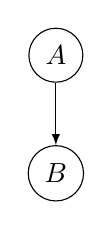
\begin{tikzpicture}[edge from parent/.style={draw,-latex}]
        \node[draw,circle] {$A$}
        child {node[draw,circle] {$B$}};
      \end{tikzpicture}
    \end{subfigure}%
    \begin{subfigure}{0.8\textwidth}
      \centering
      \begin{tabular}[t]{cc}
        \toprule
        $a$ & $\Pr(A = a)$ \\
        \midrule
        1 & 0.5 \\
        0 & 0.5 \\
        \bottomrule
      \end{tabular}
      \begin{tabular}[t]{ccc}
        \toprule
        $a$ & $b$ & $\Pr(B = b \mid A = a)$ \\
        \midrule
        1 & 1 & 0.6 \\
        1 & 0 & 0.4 \\
        0 & 1 & 0.1 \\
        0 & 0 & 0.9 \\
        \bottomrule
      \end{tabular}
    \end{subfigure}
    \caption{A Bayesian network with its conditional probability tables}
  \end{figure}
  \pause
  Let \structure{$U = \{ \lambda_{A=1}, \lambda_{B=1} \}$}. The weight function
  \structure{$\nu\colon 2^U \to \mathbb{R}_{\ge 0}$} for this network can be
  defined as \structure{$\nu \coloneqq \nu_A \cdot \nu_B$}, where
  \structure{$\nu_A = 0.5$}, and
  \begin{align*}
    \nu_B &= 0.6[\lambda_{B=1}] \cdot [\lambda_{A=1}] + 0.4\overline{[\lambda_{B=1}]} \cdot [\lambda_{A=1}] \\
          &+ 0.1[\lambda_{B=1}] \cdot \overline{[\lambda_{A=1}]} + 0.9\overline{[\lambda_{B=1}]} \cdot \overline{[\lambda_{A=1}]}.
  \end{align*}
\end{frame}

\begin{frame}{Experimental Results}
  \centering
  \scalebox{0.8}{% Created by tikzDevice version 0.12.3 on 2020-08-01 17:20:52
% !TEX encoding = UTF-8 Unicode
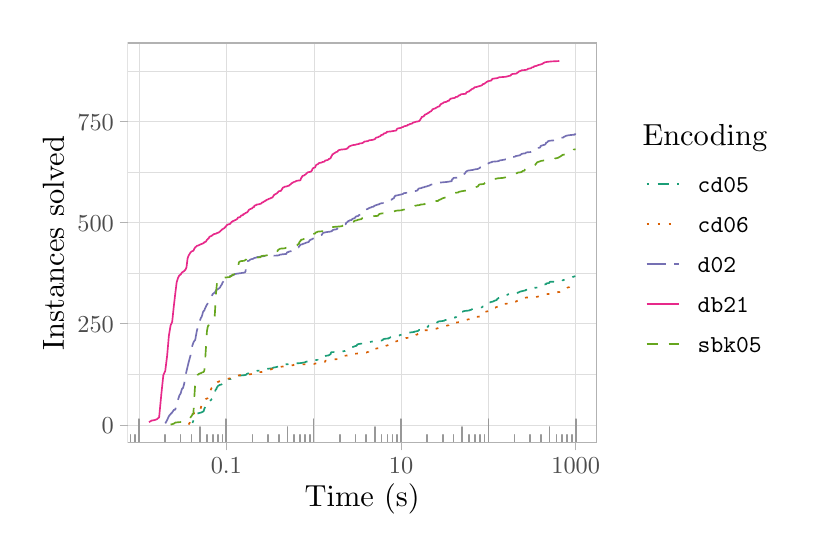
\begin{tikzpicture}[x=1pt,y=1pt]
\definecolor{fillColor}{RGB}{255,255,255}
\path[use as bounding box,fill=fillColor,fill opacity=0.00] (0,0) rectangle (278.24,180.67);
\begin{scope}
\path[clip] (  0.00,  0.00) rectangle (278.24,180.67);
\definecolor{drawColor}{RGB}{255,255,255}
\definecolor{fillColor}{RGB}{255,255,255}

\path[draw=drawColor,line width= 0.6pt,line join=round,line cap=round,fill=fillColor] (  0.00,  0.00) rectangle (278.24,180.68);
\end{scope}
\begin{scope}
\path[clip] ( 36.11, 30.69) rectangle (205.68,175.17);
\definecolor{fillColor}{RGB}{255,255,255}

\path[fill=fillColor] ( 36.11, 30.69) rectangle (205.68,175.17);
\definecolor{drawColor}{gray}{0.87}

\path[draw=drawColor,line width= 0.1pt,line join=round] ( 36.11, 55.37) --
	(205.68, 55.37);

\path[draw=drawColor,line width= 0.1pt,line join=round] ( 36.11, 91.90) --
	(205.68, 91.90);

\path[draw=drawColor,line width= 0.1pt,line join=round] ( 36.11,128.43) --
	(205.68,128.43);

\path[draw=drawColor,line width= 0.1pt,line join=round] ( 36.11,164.95) --
	(205.68,164.95);

\path[draw=drawColor,line width= 0.1pt,line join=round] ( 40.22, 30.69) --
	( 40.22,175.17);

\path[draw=drawColor,line width= 0.1pt,line join=round] (103.34, 30.69) --
	(103.34,175.17);

\path[draw=drawColor,line width= 0.1pt,line join=round] (166.47, 30.69) --
	(166.47,175.17);

\path[draw=drawColor,line width= 0.3pt,line join=round] ( 36.11, 37.11) --
	(205.68, 37.11);

\path[draw=drawColor,line width= 0.3pt,line join=round] ( 36.11, 73.64) --
	(205.68, 73.64);

\path[draw=drawColor,line width= 0.3pt,line join=round] ( 36.11,110.16) --
	(205.68,110.16);

\path[draw=drawColor,line width= 0.3pt,line join=round] ( 36.11,146.69) --
	(205.68,146.69);

\path[draw=drawColor,line width= 0.3pt,line join=round] ( 71.78, 30.69) --
	( 71.78,175.17);

\path[draw=drawColor,line width= 0.3pt,line join=round] (134.91, 30.69) --
	(134.91,175.17);

\path[draw=drawColor,line width= 0.3pt,line join=round] (198.03, 30.69) --
	(198.03,175.17);
\definecolor{drawColor}{RGB}{27,158,119}

\path[draw=drawColor,line width= 0.6pt,dash pattern=on 1pt off 3pt on 4pt off 3pt ,line join=round] ( 59.56, 37.84) --
	( 59.89, 38.71) --
	( 60.22, 39.74) --
	( 60.53, 40.47) --
	( 60.84, 40.91) --
	( 61.14, 41.20) --
	( 62.82, 41.64) --
	( 63.59, 42.08) --
	( 63.84, 42.95) --
	( 64.08, 43.54) --
	( 64.32, 44.41) --
	( 64.55, 44.85) --
	( 64.78, 45.14) --
	( 65.01, 45.29) --
	( 65.23, 45.44) --
	( 65.45, 45.58) --
	( 65.88, 45.87) --
	( 66.09, 46.02) --
	( 66.29, 46.17) --
	( 66.50, 46.46) --
	( 66.89, 46.75) --
	( 67.09, 47.34) --
	( 67.28, 47.63) --
	( 67.47, 48.07) --
	( 67.66, 48.80) --
	( 67.84, 49.67) --
	( 68.02, 49.97) --
	( 68.20, 50.11) --
	( 68.38, 50.70) --
	( 68.55, 50.84) --
	( 68.73, 51.13) --
	( 68.90, 51.28) --
	( 69.39, 51.57) --
	( 70.03, 51.72) --
	( 70.19, 51.86) --
	( 70.34, 52.01) --
	( 70.49, 52.16) --
	( 70.64, 52.60) --
	( 70.79, 52.74) --
	( 70.94, 53.03) --
	( 71.08, 53.18) --
	( 71.37, 53.33) --
	( 71.92, 53.47) --
	( 72.32, 53.62) --
	( 73.46, 53.76) --
	( 73.58, 53.91) --
	( 73.82, 54.20) --
	( 74.73, 54.35) --
	( 74.84, 54.49) --
	( 75.38, 54.64) --
	( 76.00, 54.79) --
	( 76.20, 54.93) --
	( 78.14, 55.08) --
	( 78.89, 55.23) --
	( 79.06, 55.37) --
	( 79.14, 55.52) --
	( 79.38, 55.66) --
	( 79.84, 55.81) --
	( 80.80, 55.96) --
	( 81.01, 56.10) --
	( 81.56, 56.25) --
	( 82.15, 56.39) --
	( 82.40, 56.54) --
	( 82.90, 56.69) --
	( 84.51, 56.83) --
	( 85.55, 56.98) --
	( 85.60, 57.12) --
	( 86.14, 57.27) --
	( 86.75, 57.42) --
	( 88.27, 57.56) --
	( 88.56, 57.71) --
	( 88.92, 57.86) --
	( 89.68, 58.00) --
	( 90.33, 58.15) --
	( 91.26, 58.29) --
	( 92.25, 58.44) --
	( 92.67, 58.59) --
	( 92.82, 58.73) --
	( 92.88, 58.88) --
	( 93.23, 59.02) --
	( 95.54, 59.17) --
	( 95.78, 59.32) --
	( 98.51, 59.46) --
	( 99.60, 59.61) --
	(100.18, 59.75) --
	(100.44, 59.90) --
	(100.97, 60.05) --
	(102.70, 60.19) --
	(102.77, 60.34) --
	(103.18, 60.49) --
	(104.73, 60.63) --
	(104.84, 60.78) --
	(104.86, 60.92) --
	(105.61, 61.07) --
	(105.71, 61.22) --
	(105.76, 61.36) --
	(106.49, 61.65) --
	(106.71, 61.80) --
	(107.11, 61.95) --
	(107.66, 62.09) --
	(108.70, 62.24) --
	(108.94, 62.38) --
	(109.14, 62.53) --
	(109.44, 62.68) --
	(109.53, 62.82) --
	(109.55, 62.97) --
	(109.56, 63.12) --
	(109.61, 63.26) --
	(109.79, 63.41) --
	(113.34, 63.55) --
	(113.86, 63.70) --
	(114.65, 63.85) --
	(114.85, 63.99) --
	(114.96, 64.14) --
	(115.67, 64.28) --
	(115.88, 64.43) --
	(115.93, 64.58) --
	(116.05, 64.72) --
	(116.59, 64.87) --
	(116.80, 65.01) --
	(117.01, 65.16) --
	(117.54, 65.31) --
	(117.99, 65.45) --
	(118.33, 65.60) --
	(118.91, 65.75) --
	(118.95, 65.89) --
	(119.00, 66.04) --
	(119.07, 66.18) --
	(119.49, 66.33) --
	(120.39, 66.48) --
	(122.58, 66.62) --
	(123.52, 66.77) --
	(123.65, 66.91) --
	(123.88, 67.06) --
	(124.05, 67.21) --
	(125.63, 67.35) --
	(125.97, 67.50) --
	(127.90, 67.64) --
	(128.29, 67.79) --
	(128.40, 67.94) --
	(128.51, 68.08) --
	(128.93, 68.23) --
	(130.47, 68.38) --
	(130.56, 68.52) --
	(130.91, 68.67) --
	(131.06, 68.81) --
	(132.13, 68.96) --
	(132.68, 69.11) --
	(132.88, 69.25) --
	(134.33, 69.40) --
	(134.38, 69.54) --
	(134.92, 69.69) --
	(135.51, 69.84) --
	(135.83, 69.98) --
	(136.08, 70.13) --
	(136.75, 70.27) --
	(137.17, 70.42) --
	(138.61, 70.57) --
	(139.62, 70.71) --
	(139.84, 70.86) --
	(140.77, 71.01) --
	(141.17, 71.15) --
	(141.26, 71.30) --
	(141.42, 71.44) --
	(143.11, 71.59) --
	(143.19, 71.74) --
	(143.46, 71.88) --
	(144.14, 72.03) --
	(144.34, 72.17) --
	(144.37, 72.32) --
	(144.48, 72.47) --
	(144.58, 72.61) --
	(144.79, 72.76) --
	(144.81, 72.90) --
	(144.95, 73.05) --
	(145.24, 73.20) --
	(145.47, 73.34) --
	(145.92, 73.49) --
	(147.23, 73.64) --
	(147.44, 73.78) --
	(147.46, 73.93) --
	(147.72, 74.07) --
	(148.22, 74.22) --
	(148.27, 74.37) --
	(148.30, 74.51) --
	(149.81, 74.66) --
	(150.57, 74.80) --
	(150.66, 74.95) --
	(151.33, 75.10) --
	(151.51, 75.24) --
	(151.72, 75.39) --
	(152.00, 75.53) --
	(152.11, 75.68) --
	(152.77, 75.83) --
	(154.61, 75.97) --
	(154.83, 76.12) --
	(154.90, 76.27) --
	(154.95, 76.41) --
	(155.00, 76.56) --
	(155.20, 76.70) --
	(155.26, 76.85) --
	(155.28, 77.00) --
	(155.81, 77.14) --
	(155.83, 77.29) --
	(155.95, 77.43) --
	(156.19, 77.58) --
	(156.23, 77.73) --
	(156.33, 77.87) --
	(157.14, 78.02) --
	(157.39, 78.16) --
	(158.01, 78.31) --
	(159.50, 78.46) --
	(159.73, 78.60) --
	(160.29, 78.75) --
	(160.47, 78.90) --
	(161.11, 79.04) --
	(161.73, 79.19) --
	(162.65, 79.33) --
	(163.23, 79.48) --
	(164.16, 79.63) --
	(164.29, 79.77) --
	(164.53, 79.92) --
	(165.13, 80.06) --
	(165.72, 80.21) --
	(165.75, 80.36) --
	(165.77, 80.50) --
	(166.15, 80.65) --
	(166.22, 80.79) --
	(166.27, 80.94) --
	(166.35, 81.09) --
	(166.35, 81.23) --
	(167.05, 81.38) --
	(167.35, 81.53) --
	(168.04, 81.67) --
	(168.37, 81.82) --
	(168.61, 81.96) --
	(169.05, 82.11) --
	(169.51, 82.26) --
	(169.52, 82.40) --
	(169.62, 82.55) --
	(169.80, 82.69) --
	(169.96, 82.84) --
	(170.15, 82.99) --
	(170.56, 83.13) --
	(170.65, 83.28) --
	(170.96, 83.42) --
	(171.94, 83.57) --
	(172.12, 83.72) --
	(172.36, 83.86) --
	(172.47, 84.01) --
	(173.42, 84.16) --
	(173.44, 84.30) --
	(175.96, 84.45) --
	(176.63, 84.59) --
	(176.97, 84.74) --
	(176.99, 84.89) --
	(177.55, 85.03) --
	(177.57, 85.18) --
	(178.08, 85.32) --
	(178.68, 85.47) --
	(179.32, 85.62) --
	(179.91, 85.76) --
	(180.02, 85.91) --
	(181.06, 86.05) --
	(181.14, 86.20) --
	(181.21, 86.35) --
	(182.87, 86.49) --
	(182.94, 86.64) --
	(184.41, 86.79) --
	(184.74, 86.93) --
	(184.93, 87.08) --
	(185.23, 87.22) --
	(185.27, 87.37) --
	(185.96, 87.52) --
	(186.07, 87.66) --
	(186.19, 87.81) --
	(187.31, 87.95) --
	(187.35, 88.10) --
	(187.37, 88.25) --
	(188.44, 88.39) --
	(188.53, 88.54) --
	(188.55, 88.68) --
	(188.68, 88.83) --
	(192.45, 88.98) --
	(193.20, 89.12) --
	(193.28, 89.27) --
	(193.38, 89.42) --
	(193.89, 89.56) --
	(194.14, 89.71) --
	(194.52, 89.85) --
	(195.52, 90.00) --
	(195.91, 90.15) --
	(196.52, 90.29) --
	(196.72, 90.44) --
	(196.95, 90.58) --
	(197.43, 90.73) --
	(197.91, 90.88);
\definecolor{drawColor}{RGB}{217,95,2}

\path[draw=drawColor,line width= 0.6pt,dash pattern=on 1pt off 3pt ,line join=round] ( 58.16, 37.25) --
	( 58.52, 37.84) --
	( 58.88, 39.59) --
	( 59.22, 40.47) --
	( 59.56, 41.05) --
	( 60.22, 41.34) --
	( 61.14, 41.49) --
	( 61.43, 41.78) --
	( 62.01, 41.93) --
	( 62.28, 42.08) --
	( 62.55, 43.24) --
	( 62.82, 44.27) --
	( 63.08, 44.85) --
	( 63.34, 45.44) --
	( 63.84, 45.87) --
	( 64.08, 46.02) --
	( 64.32, 46.46) --
	( 65.01, 46.75) --
	( 65.23, 46.90) --
	( 65.45, 47.34) --
	( 65.67, 47.77) --
	( 65.88, 48.65) --
	( 66.09, 49.53) --
	( 66.29, 50.11) --
	( 66.50, 50.55) --
	( 66.70, 50.84) --
	( 66.89, 51.43) --
	( 67.09, 51.57) --
	( 67.28, 51.72) --
	( 67.47, 51.86) --
	( 67.84, 52.01) --
	( 68.02, 52.16) --
	( 68.38, 52.30) --
	( 68.55, 52.60) --
	( 69.06, 52.74) --
	( 69.23, 52.89) --
	( 69.56, 53.03) --
	( 69.87, 53.18) --
	( 70.19, 53.33) --
	( 70.94, 53.47) --
	( 71.65, 53.62) --
	( 71.78, 53.76) --
	( 72.97, 53.91) --
	( 73.46, 54.06) --
	( 73.82, 54.20) --
	( 74.28, 54.49) --
	( 74.84, 54.64) --
	( 74.95, 54.79) --
	( 75.49, 54.93) --
	( 76.59, 55.08) --
	( 79.22, 55.23) --
	( 79.84, 55.37) --
	( 81.01, 55.52) --
	( 81.08, 55.66) --
	( 81.15, 55.81) --
	( 82.34, 55.96) --
	( 82.72, 56.10) --
	( 84.56, 56.25) --
	( 85.50, 56.39) --
	( 86.19, 56.54) --
	( 86.47, 56.69) --
	( 87.11, 56.83) --
	( 87.34, 56.98) --
	( 87.73, 57.12) --
	( 88.11, 57.27) --
	( 88.44, 57.42) --
	( 88.72, 57.56) --
	( 90.61, 57.86) --
	( 90.85, 58.00) --
	( 91.55, 58.15) --
	( 92.76, 58.29) --
	( 93.82, 58.44) --
	( 94.85, 58.59) --
	( 96.09, 58.73) --
	( 96.16, 58.88) --
	(100.27, 59.02) --
	(103.56, 59.17) --
	(103.99, 59.32) --
	(104.98, 59.46) --
	(105.40, 59.61) --
	(106.51, 59.75) --
	(107.46, 59.90) --
	(107.47, 60.05) --
	(107.50, 60.19) --
	(107.71, 60.34) --
	(108.64, 60.49) --
	(109.52, 60.63) --
	(110.62, 60.78) --
	(112.04, 60.92) --
	(112.14, 61.07) --
	(112.60, 61.22) --
	(112.83, 61.36) --
	(113.18, 61.51) --
	(113.48, 61.65) --
	(113.88, 61.80) --
	(114.05, 61.95) --
	(114.28, 62.09) --
	(115.62, 62.24) --
	(117.04, 62.38) --
	(117.14, 62.53) --
	(117.17, 62.68) --
	(117.61, 62.82) --
	(120.08, 62.97) --
	(120.83, 63.12) --
	(122.39, 63.26) --
	(122.72, 63.41) --
	(123.16, 63.55) --
	(123.21, 63.70) --
	(123.36, 63.85) --
	(123.36, 63.99) --
	(123.39, 64.14) --
	(123.45, 64.28) --
	(123.90, 64.43) --
	(125.26, 64.58) --
	(126.04, 64.72) --
	(126.78, 64.87) --
	(126.86, 65.01) --
	(126.88, 65.16) --
	(127.97, 65.31) --
	(128.41, 65.45) --
	(129.17, 65.60) --
	(129.56, 65.75) --
	(130.06, 65.89) --
	(130.38, 66.04) --
	(130.54, 66.18) --
	(130.85, 66.33) --
	(130.89, 66.48) --
	(131.15, 66.62) --
	(131.28, 66.77) --
	(132.02, 66.91) --
	(132.22, 67.06) --
	(132.44, 67.21) --
	(133.43, 67.35) --
	(133.58, 67.50) --
	(134.96, 67.64) --
	(135.14, 67.79) --
	(135.24, 67.94) --
	(135.48, 68.08) --
	(135.83, 68.23) --
	(136.36, 68.38) --
	(136.68, 68.52) --
	(138.14, 68.67) --
	(138.61, 68.81) --
	(139.38, 68.96) --
	(139.38, 69.11) --
	(139.57, 69.25) --
	(139.89, 69.40) --
	(140.07, 69.54) --
	(140.31, 69.69) --
	(140.91, 69.84) --
	(140.91, 69.98) --
	(141.45, 70.13) --
	(141.90, 70.27) --
	(142.10, 70.42) --
	(142.92, 70.57) --
	(143.07, 70.71) --
	(143.09, 70.86) --
	(143.28, 71.01) --
	(143.30, 71.15) --
	(143.55, 71.30) --
	(145.67, 71.44) --
	(145.79, 71.59) --
	(146.91, 71.74) --
	(147.53, 71.88) --
	(148.12, 72.03) --
	(148.43, 72.17) --
	(149.21, 72.32) --
	(149.80, 72.47) --
	(149.98, 72.61) --
	(150.56, 72.76) --
	(150.83, 72.90) --
	(151.81, 73.05) --
	(152.13, 73.20) --
	(152.20, 73.34) --
	(152.27, 73.49) --
	(152.29, 73.64) --
	(152.51, 73.78) --
	(153.79, 73.93) --
	(154.57, 74.07) --
	(155.62, 74.22) --
	(156.39, 74.37) --
	(156.92, 74.51) --
	(157.40, 74.66) --
	(157.72, 74.80) --
	(158.16, 74.95) --
	(158.71, 75.10) --
	(159.02, 75.24) --
	(160.09, 75.39) --
	(161.11, 75.53) --
	(161.61, 75.68) --
	(161.61, 75.83) --
	(161.64, 75.97) --
	(161.96, 76.12) --
	(163.07, 76.27) --
	(163.87, 76.41) --
	(164.09, 76.56) --
	(164.16, 76.70) --
	(164.19, 76.85) --
	(164.19, 77.00) --
	(164.27, 77.14) --
	(164.36, 77.29) --
	(164.37, 77.43) --
	(164.74, 77.58) --
	(164.89, 77.73) --
	(165.08, 77.87) --
	(165.27, 78.02) --
	(166.19, 78.16) --
	(166.53, 78.31) --
	(167.14, 78.46) --
	(167.22, 78.60) --
	(167.32, 78.75) --
	(167.41, 78.90) --
	(167.47, 79.04) --
	(167.60, 79.19) --
	(168.37, 79.33) --
	(168.97, 79.48) --
	(169.19, 79.63) --
	(169.60, 79.77) --
	(169.95, 79.92) --
	(170.05, 80.06) --
	(170.07, 80.21) --
	(170.29, 80.36) --
	(170.32, 80.50) --
	(171.11, 80.65) --
	(172.05, 80.79) --
	(173.03, 80.94) --
	(174.96, 81.09) --
	(175.34, 81.23) --
	(175.36, 81.38) --
	(175.59, 81.53) --
	(176.49, 81.67) --
	(176.54, 81.82) --
	(176.94, 81.96) --
	(177.77, 82.11) --
	(178.02, 82.26) --
	(178.10, 82.40) --
	(178.99, 82.55) --
	(179.08, 82.69) --
	(179.24, 82.84) --
	(179.51, 82.99) --
	(179.99, 83.13) --
	(183.14, 83.28) --
	(183.99, 83.42) --
	(184.68, 83.57) --
	(185.02, 83.72) --
	(185.75, 83.86) --
	(186.49, 84.01) --
	(186.80, 84.16) --
	(187.12, 84.30) --
	(188.18, 84.45) --
	(190.60, 84.59) --
	(190.74, 84.74) --
	(190.94, 84.89) --
	(191.10, 85.03) --
	(192.25, 85.18) --
	(192.34, 85.32) --
	(192.58, 85.47) --
	(192.67, 85.62) --
	(193.26, 85.76) --
	(193.55, 85.91) --
	(194.02, 86.05) --
	(194.49, 86.20) --
	(194.66, 86.35) --
	(194.75, 86.49) --
	(194.92, 86.64) --
	(195.22, 86.79) --
	(195.70, 86.93) --
	(195.72, 87.08) --
	(195.89, 87.22) --
	(196.24, 87.37) --
	(196.29, 87.52) --
	(196.68, 87.66);
\definecolor{drawColor}{RGB}{117,112,179}

\path[draw=drawColor,line width= 0.6pt,dash pattern=on 7pt off 3pt ,line join=round] ( 49.72, 37.69) --
	( 50.39, 38.86) --
	( 51.03, 40.32) --
	( 51.64, 41.05) --
	( 52.22, 41.64) --
	( 52.78, 42.51) --
	( 53.32, 42.66) --
	( 53.84, 44.56) --
	( 54.34, 46.31) --
	( 54.82, 47.77) --
	( 55.28, 48.50) --
	( 55.73, 50.11) --
	( 56.17, 50.55) --
	( 56.59, 52.16) --
	( 57.00, 54.93) --
	( 57.39, 56.54) --
	( 57.78, 58.15) --
	( 58.16, 59.75) --
	( 58.52, 61.07) --
	( 58.88, 62.38) --
	( 59.22, 64.87) --
	( 59.56, 65.89) --
	( 59.89, 66.91) --
	( 60.22, 67.50) --
	( 60.53, 67.79) --
	( 60.84, 69.54) --
	( 61.14, 71.15) --
	( 61.43, 72.17) --
	( 61.72, 73.49) --
	( 62.01, 74.07) --
	( 62.28, 74.95) --
	( 62.55, 75.68) --
	( 62.82, 76.12) --
	( 63.08, 76.85) --
	( 63.34, 77.87) --
	( 63.59, 78.31) --
	( 63.84, 78.46) --
	( 64.08, 79.19) --
	( 64.32, 79.63) --
	( 64.55, 80.21) --
	( 65.01, 80.94) --
	( 65.23, 81.38) --
	( 65.45, 81.82) --
	( 65.67, 82.40) --
	( 65.88, 82.84) --
	( 66.09, 83.28) --
	( 66.29, 83.57) --
	( 66.50, 83.86) --
	( 66.70, 84.01) --
	( 66.89, 84.45) --
	( 67.09, 84.59) --
	( 67.28, 84.74) --
	( 67.66, 85.03) --
	( 67.84, 85.32) --
	( 68.02, 85.76) --
	( 68.20, 85.91) --
	( 68.55, 86.05) --
	( 68.73, 86.20) --
	( 69.39, 86.64) --
	( 69.56, 86.93) --
	( 69.72, 87.22) --
	( 69.87, 87.52) --
	( 70.03, 87.66) --
	( 70.19, 87.95) --
	( 70.34, 88.39) --
	( 70.49, 88.68) --
	( 70.64, 88.83) --
	( 70.79, 89.12) --
	( 71.08, 89.27) --
	( 71.22, 89.42) --
	( 71.37, 89.85) --
	( 71.65, 90.00) --
	( 71.78, 90.15) --
	( 71.92, 90.29) --
	( 72.06, 90.44) --
	( 72.45, 90.58) --
	( 72.58, 90.73) --
	( 72.97, 90.88) --
	( 73.34, 91.02) --
	( 73.94, 91.17) --
	( 74.40, 91.31) --
	( 74.62, 91.46) --
	( 74.73, 91.61) --
	( 75.49, 91.75) --
	( 76.49, 91.90) --
	( 78.48, 92.19) --
	( 78.73, 92.63) --
	( 78.81, 93.51) --
	( 78.89, 93.80) --
	( 78.98, 94.68) --
	( 79.06, 95.26) --
	( 79.14, 95.84) --
	( 79.22, 96.14) --
	( 79.30, 96.28) --
	( 79.84, 96.43) --
	( 80.14, 96.57) --
	( 80.22, 96.72) --
	( 80.44, 96.87) --
	( 80.80, 97.01) --
	( 81.49, 97.16) --
	( 81.89, 97.45) --
	( 82.65, 97.60) --
	( 82.84, 97.74) --
	( 83.90, 97.89) --
	( 84.45, 98.04) --
	( 86.33, 98.18) --
	( 90.23, 98.33) --
	( 90.89, 98.47) --
	( 91.09, 98.62) --
	( 92.03, 98.77) --
	( 93.45, 98.91) --
	( 93.54, 99.06) --
	( 93.60, 99.20) --
	( 93.68, 99.35) --
	( 93.73, 99.50) --
	( 94.33, 99.64) --
	( 94.49, 99.79) --
	( 95.47, 99.94) --
	( 95.88,100.08) --
	( 96.14,100.23) --
	( 96.18,100.37) --
	( 96.21,100.52) --
	( 96.32,100.67) --
	( 96.39,100.81) --
	( 96.86,100.96) --
	( 97.21,101.10) --
	( 97.92,101.25) --
	( 97.96,101.54) --
	( 98.18,101.69) --
	( 98.22,101.83) --
	( 98.42,101.98) --
	( 98.46,102.13) --
	( 98.51,102.27) --
	( 99.37,102.42) --
	( 99.53,102.57) --
	(100.03,102.71) --
	(100.41,102.86) --
	(100.71,103.00) --
	(101.28,103.15) --
	(101.65,103.30) --
	(101.67,103.44) --
	(101.75,103.59) --
	(101.78,103.73) --
	(102.02,103.88) --
	(102.14,104.03) --
	(102.71,104.17) --
	(102.84,104.32) --
	(103.10,104.46) --
	(103.52,104.61) --
	(103.56,104.76) --
	(103.82,104.90) --
	(104.18,105.05) --
	(104.65,105.20) --
	(104.75,105.34) --
	(104.92,105.49) --
	(105.22,105.63) --
	(106.18,105.78) --
	(106.45,105.93) --
	(106.46,106.07) --
	(106.51,106.22) --
	(106.59,106.36) --
	(106.79,106.51) --
	(107.32,106.66) --
	(107.97,106.80) --
	(109.12,106.95) --
	(109.80,107.09) --
	(109.95,107.24) --
	(110.13,107.39) --
	(110.22,107.53) --
	(110.65,107.68) --
	(111.64,107.83) --
	(111.78,107.97) --
	(111.95,108.12) --
	(112.27,108.26) --
	(112.36,108.41) --
	(112.47,108.56) --
	(112.69,108.70) --
	(113.03,108.85) --
	(114.03,108.99) --
	(114.08,109.14) --
	(114.37,109.29) --
	(114.57,109.43) --
	(114.79,109.58) --
	(114.97,109.72) --
	(115.02,109.87) --
	(115.04,110.02) --
	(115.06,110.16) --
	(115.34,110.31) --
	(115.59,110.46) --
	(115.77,110.75) --
	(116.16,110.89) --
	(116.35,111.04) --
	(117.07,111.19) --
	(117.12,111.33) --
	(117.28,111.48) --
	(117.45,111.62) --
	(117.98,111.77) --
	(118.20,111.92) --
	(118.36,112.06) --
	(118.39,112.21) --
	(118.53,112.35) --
	(118.78,112.50) --
	(119.53,112.65) --
	(119.57,112.79) --
	(119.71,112.94) --
	(120.24,113.09) --
	(120.43,113.23) --
	(120.58,113.38) --
	(120.81,113.52) --
	(120.97,113.67) --
	(121.10,113.82) --
	(121.14,113.96) --
	(121.40,114.11) --
	(121.75,114.25) --
	(121.90,114.40) --
	(121.92,114.55) --
	(122.03,114.69) --
	(122.04,114.84) --
	(122.28,114.98) --
	(122.73,115.13) --
	(123.10,115.28) --
	(123.21,115.42) --
	(123.55,115.57) --
	(124.13,115.72) --
	(124.25,115.86) --
	(125.09,116.01) --
	(125.12,116.15) --
	(125.21,116.30) --
	(125.70,116.45) --
	(126.00,116.59) --
	(126.50,116.74) --
	(127.06,116.88) --
	(127.13,117.03) --
	(127.65,117.18) --
	(128.70,117.32) --
	(128.88,117.47) --
	(129.48,117.61) --
	(129.52,117.76) --
	(129.82,117.91) --
	(129.97,118.05) --
	(130.10,118.20) --
	(130.58,118.35) --
	(131.41,118.49) --
	(131.72,118.64) --
	(131.73,118.78) --
	(132.11,118.93) --
	(132.37,119.08) --
	(132.41,119.22) --
	(132.42,119.37) --
	(132.49,119.51) --
	(132.72,119.66) --
	(132.72,119.81) --
	(132.75,119.95) --
	(133.66,120.10) --
	(134.25,120.24) --
	(134.93,120.39) --
	(135.48,120.54) --
	(135.77,120.68) --
	(135.79,120.83) --
	(136.82,120.98) --
	(138.98,121.12) --
	(139.04,121.27) --
	(139.29,121.41) --
	(139.48,121.56) --
	(140.44,121.71) --
	(140.86,121.85) --
	(140.91,122.00) --
	(141.03,122.14) --
	(141.08,122.29) --
	(141.19,122.44) --
	(141.46,122.58) --
	(142.34,122.73) --
	(142.44,122.87) --
	(143.30,123.02) --
	(143.50,123.17) --
	(144.24,123.31) --
	(144.60,123.46) --
	(145.17,123.61) --
	(145.40,123.75) --
	(145.59,123.90) --
	(146.20,124.04) --
	(146.25,124.19) --
	(146.60,124.34) --
	(147.98,124.48) --
	(148.31,124.63) --
	(149.79,124.77) --
	(151.46,124.92) --
	(152.37,125.07) --
	(153.22,125.21) --
	(153.24,125.36) --
	(153.25,125.50) --
	(153.31,125.65) --
	(153.37,125.80) --
	(153.51,125.94) --
	(153.74,126.09) --
	(153.76,126.24) --
	(153.92,126.38) --
	(155.79,126.53) --
	(155.99,126.67) --
	(156.04,126.82) --
	(156.04,126.97) --
	(156.06,127.11) --
	(156.08,127.26) --
	(156.62,127.40) --
	(156.85,127.55) --
	(157.50,127.70) --
	(157.82,127.84) --
	(157.99,127.99) --
	(158.09,128.13) --
	(158.18,128.28) --
	(158.30,128.43) --
	(158.32,128.57) --
	(158.55,128.72) --
	(158.76,128.87) --
	(159.03,129.01) --
	(160.11,129.16) --
	(161.06,129.30) --
	(161.46,129.45) --
	(162.59,129.60) --
	(162.89,129.74) --
	(163.16,129.89) --
	(163.42,130.03) --
	(163.50,130.18) --
	(164.13,130.33) --
	(164.20,130.47) --
	(164.21,130.62) --
	(165.03,130.76) --
	(165.20,130.91) --
	(165.51,131.06) --
	(165.65,131.20) --
	(165.73,131.35) --
	(165.97,131.50) --
	(166.64,131.64) --
	(166.66,131.79) --
	(167.17,131.93) --
	(167.70,132.08) --
	(167.82,132.23) --
	(169.68,132.37) --
	(170.34,132.52) --
	(170.38,132.66) --
	(171.34,132.81) --
	(172.16,132.96) --
	(172.76,133.10) --
	(174.66,133.25) --
	(174.70,133.39) --
	(174.80,133.54) --
	(174.87,133.69) --
	(175.14,133.83) --
	(175.66,133.98) --
	(176.26,134.13) --
	(176.37,134.27) --
	(177.25,134.42) --
	(177.92,134.56) --
	(177.99,134.71) --
	(178.29,134.86) --
	(178.40,135.00) --
	(178.89,135.15) --
	(179.91,135.29) --
	(180.01,135.44) --
	(180.14,135.59) --
	(181.73,135.73) --
	(181.96,135.88) --
	(182.22,136.02) --
	(182.93,136.17) --
	(183.17,136.32) --
	(183.41,136.46) --
	(183.58,136.61) --
	(184.30,136.76) --
	(184.33,136.90) --
	(184.47,137.05) --
	(184.50,137.19) --
	(185.12,137.34) --
	(185.22,137.49) --
	(185.26,137.63) --
	(185.32,137.78) --
	(185.34,137.92) --
	(185.80,138.07) --
	(186.21,138.22) --
	(186.89,138.36) --
	(186.98,138.51) --
	(187.10,138.65) --
	(187.27,138.80) --
	(187.27,138.95) --
	(187.31,139.09) --
	(187.68,139.24) --
	(187.91,139.39) --
	(187.92,139.53) --
	(188.12,139.68) --
	(188.71,139.82) --
	(190.50,139.97) --
	(190.82,140.12) --
	(191.62,140.26) --
	(191.66,140.41) --
	(192.27,140.55) --
	(192.48,140.70) --
	(192.66,140.85) --
	(193.59,140.99) --
	(193.66,141.14) --
	(193.94,141.28) --
	(194.26,141.43) --
	(194.47,141.58) --
	(195.06,141.72) --
	(196.16,141.87) --
	(197.75,142.02) --
	(197.84,142.16) --
	(197.88,142.31) --
	(197.96,142.45);
\definecolor{drawColor}{RGB}{231,41,138}

\path[draw=drawColor,line width= 0.6pt,line join=round] ( 43.82, 38.13) --
	( 44.83, 38.71) --
	( 45.78, 38.86) --
	( 46.66, 39.15) --
	( 47.50, 39.88) --
	( 48.28, 48.07) --
	( 49.02, 55.08) --
	( 49.72, 56.69) --
	( 50.39, 62.09) --
	( 51.03, 69.40) --
	( 51.64, 73.05) --
	( 52.22, 74.37) --
	( 52.78, 79.77) --
	( 53.32, 84.45) --
	( 53.84, 88.68) --
	( 54.34, 90.29) --
	( 54.82, 91.17) --
	( 55.28, 91.46) --
	( 55.73, 92.19) --
	( 56.59, 92.78) --
	( 57.00, 93.21) --
	( 57.39, 94.09) --
	( 57.78, 97.31) --
	( 58.16, 98.33) --
	( 58.52, 98.91) --
	( 58.88, 99.50) --
	( 59.22, 99.79) --
	( 59.89,100.08) --
	( 60.22,100.81) --
	( 60.53,101.25) --
	( 60.84,101.54) --
	( 61.14,101.83) --
	( 61.72,101.98) --
	( 62.01,102.13) --
	( 62.28,102.27) --
	( 62.55,102.42) --
	( 63.08,102.57) --
	( 63.34,102.71) --
	( 63.59,102.86) --
	( 63.84,103.15) --
	( 64.32,103.30) --
	( 64.55,103.59) --
	( 64.78,104.03) --
	( 65.01,104.17) --
	( 65.23,104.46) --
	( 65.45,104.61) --
	( 65.67,105.05) --
	( 65.88,105.20) --
	( 66.29,105.34) --
	( 66.50,105.49) --
	( 66.70,105.63) --
	( 67.28,106.07) --
	( 68.02,106.22) --
	( 68.20,106.36) --
	( 68.55,106.51) --
	( 69.06,106.66) --
	( 69.39,106.95) --
	( 69.72,107.24) --
	( 69.87,107.39) --
	( 70.03,107.53) --
	( 70.19,107.68) --
	( 70.34,107.83) --
	( 70.64,107.97) --
	( 71.08,108.26) --
	( 71.22,108.41) --
	( 71.37,108.56) --
	( 71.51,108.70) --
	( 71.65,108.85) --
	( 71.92,109.29) --
	( 72.45,109.58) --
	( 73.09,109.72) --
	( 73.21,109.87) --
	( 73.34,110.02) --
	( 73.46,110.16) --
	( 73.70,110.46) --
	( 73.94,110.60) --
	( 74.05,110.75) --
	( 74.51,110.89) --
	( 74.73,111.04) --
	( 75.17,111.19) --
	( 75.38,111.33) --
	( 75.59,111.48) --
	( 75.80,111.62) --
	( 75.90,111.92) --
	( 76.00,112.06) --
	( 76.69,112.21) --
	( 76.88,112.35) --
	( 77.06,112.65) --
	( 77.16,112.79) --
	( 77.79,112.94) --
	( 77.88,113.23) --
	( 78.23,113.38) --
	( 78.56,113.52) --
	( 78.65,113.67) --
	( 79.06,113.82) --
	( 79.38,113.96) --
	( 79.45,114.11) --
	( 79.69,114.40) --
	( 79.76,114.55) --
	( 79.84,114.69) --
	( 79.92,114.84) --
	( 80.14,114.98) --
	( 80.44,115.13) --
	( 80.87,115.28) --
	( 81.15,115.42) --
	( 81.35,115.72) --
	( 81.82,115.86) --
	( 81.89,116.30) --
	( 82.21,116.45) --
	( 82.59,116.59) --
	( 82.72,116.74) --
	( 83.67,116.88) --
	( 84.12,117.03) --
	( 84.51,117.18) --
	( 84.56,117.32) --
	( 84.67,117.47) --
	( 85.14,117.61) --
	( 85.24,117.76) --
	( 85.55,117.91) --
	( 85.75,118.05) --
	( 86.09,118.20) --
	( 86.19,118.35) --
	( 86.47,118.49) --
	( 86.89,118.64) --
	( 87.07,118.78) --
	( 87.60,118.93) --
	( 87.77,119.08) --
	( 88.23,119.22) --
	( 88.40,119.37) --
	( 88.60,119.51) --
	( 88.72,119.66) --
	( 88.76,119.81) --
	( 88.84,119.95) --
	( 88.96,120.10) --
	( 89.07,120.24) --
	( 89.30,120.39) --
	( 89.57,120.54) --
	( 90.08,120.83) --
	( 90.26,120.98) --
	( 90.40,121.12) --
	( 90.54,121.41) --
	( 90.79,121.56) --
	( 91.52,121.71) --
	( 91.62,121.85) --
	( 91.68,122.00) --
	( 91.87,122.29) --
	( 92.00,122.44) --
	( 92.06,122.58) --
	( 92.25,122.87) --
	( 92.70,123.02) --
	( 92.76,123.17) --
	( 93.60,123.31) --
	( 93.98,123.46) --
	( 94.56,123.61) --
	( 94.59,123.75) --
	( 94.69,123.90) --
	( 95.05,124.04) --
	( 95.15,124.19) --
	( 95.20,124.34) --
	( 95.40,124.48) --
	( 95.83,124.63) --
	( 95.88,124.77) --
	( 96.23,124.92) --
	( 96.75,125.07) --
	( 96.92,125.21) --
	( 97.31,125.36) --
	( 98.48,125.50) --
	( 98.59,125.65) --
	( 98.69,125.94) --
	( 98.75,126.09) --
	( 98.86,126.38) --
	( 99.01,126.53) --
	( 99.05,126.67) --
	( 99.20,126.82) --
	( 99.22,126.97) --
	( 99.31,127.11) --
	( 99.85,127.26) --
	( 99.99,127.40) --
	(100.30,127.55) --
	(100.51,127.70) --
	(100.61,127.84) --
	(100.72,127.99) --
	(100.92,128.13) --
	(101.10,128.28) --
	(101.29,128.43) --
	(102.13,128.57) --
	(102.48,128.72) --
	(102.58,128.87) --
	(102.61,129.01) --
	(102.73,129.16) --
	(102.81,129.30) --
	(102.83,129.45) --
	(102.90,129.60) --
	(103.00,129.74) --
	(103.12,129.89) --
	(103.41,130.03) --
	(103.83,130.18) --
	(103.92,130.33) --
	(104.01,130.47) --
	(104.05,130.62) --
	(104.08,130.76) --
	(104.13,130.91) --
	(104.29,131.06) --
	(104.51,131.20) --
	(104.87,131.35) --
	(105.04,131.50) --
	(105.16,131.64) --
	(105.36,131.79) --
	(106.30,131.93) --
	(106.32,132.08) --
	(107.06,132.23) --
	(107.34,132.37) --
	(107.40,132.52) --
	(107.44,132.66) --
	(108.32,132.81) --
	(108.55,132.96) --
	(108.76,133.10) --
	(108.86,133.25) --
	(109.29,133.39) --
	(109.48,133.54) --
	(109.50,133.69) --
	(109.60,133.83) --
	(109.63,133.98) --
	(109.79,134.13) --
	(109.80,134.27) --
	(109.90,134.42) --
	(110.02,134.56) --
	(110.03,134.71) --
	(110.13,134.86) --
	(110.35,135.00) --
	(110.61,135.15) --
	(110.81,135.29) --
	(111.02,135.44) --
	(111.34,135.59) --
	(111.46,135.73) --
	(112.00,135.88) --
	(112.05,136.02) --
	(112.12,136.17) --
	(112.24,136.32) --
	(112.56,136.46) --
	(113.24,136.61) --
	(114.76,136.76) --
	(115.33,136.90) --
	(115.48,137.05) --
	(115.62,137.19) --
	(115.92,137.34) --
	(115.93,137.49) --
	(115.96,137.63) --
	(116.36,137.78) --
	(116.57,137.92) --
	(116.97,138.07) --
	(117.51,138.22) --
	(118.44,138.36) --
	(118.86,138.51) --
	(119.69,138.65) --
	(119.83,138.80) --
	(120.92,138.95) --
	(121.16,139.09) --
	(121.35,139.24) --
	(121.57,139.39) --
	(121.72,139.53) --
	(122.95,139.68) --
	(123.14,139.82) --
	(123.41,139.97) --
	(124.60,140.12) --
	(125.05,140.26) --
	(125.50,140.41) --
	(125.70,140.70) --
	(125.79,140.85) --
	(126.15,140.99) --
	(126.76,141.14) --
	(126.89,141.28) --
	(127.26,141.43) --
	(127.58,141.58) --
	(127.62,141.72) --
	(127.75,141.87) --
	(128.39,142.02) --
	(128.57,142.16) --
	(128.57,142.31) --
	(128.73,142.45) --
	(129.42,142.60) --
	(129.64,142.75) --
	(129.66,142.89) --
	(129.81,143.04) --
	(131.28,143.18) --
	(132.09,143.33) --
	(133.06,143.48) --
	(133.26,143.62) --
	(133.30,143.77) --
	(133.31,143.91) --
	(133.49,144.06) --
	(133.61,144.21) --
	(134.22,144.35) --
	(135.05,144.50) --
	(135.10,144.65) --
	(135.65,144.79) --
	(135.91,144.94) --
	(136.17,145.08) --
	(137.02,145.23) --
	(137.20,145.38) --
	(137.27,145.52) --
	(137.92,145.67) --
	(137.94,145.81) --
	(138.64,145.96) --
	(139.03,146.11) --
	(139.10,146.25) --
	(139.32,146.40) --
	(139.98,146.54) --
	(140.32,146.69) --
	(141.22,146.84) --
	(141.54,146.98) --
	(141.70,147.13) --
	(141.73,147.28) --
	(141.87,147.42) --
	(141.95,147.57) --
	(141.96,147.71) --
	(142.16,147.86) --
	(142.24,148.01) --
	(142.25,148.15) --
	(142.35,148.30) --
	(142.51,148.44) --
	(143.09,148.59) --
	(143.12,148.74) --
	(143.40,148.88) --
	(143.40,149.03) --
	(143.42,149.17) --
	(143.72,149.32) --
	(144.11,149.47) --
	(144.42,149.61) --
	(144.46,149.76) --
	(144.97,149.91) --
	(145.06,150.05) --
	(145.14,150.20) --
	(145.52,150.34) --
	(145.80,150.49) --
	(145.93,150.64) --
	(146.04,150.78) --
	(146.18,150.93) --
	(146.22,151.07) --
	(146.37,151.22) --
	(146.82,151.37) --
	(147.29,151.51) --
	(147.50,151.66) --
	(147.78,151.80) --
	(147.93,151.95) --
	(148.26,152.10) --
	(148.74,152.24) --
	(148.88,152.39) --
	(148.91,152.54) --
	(149.06,152.68) --
	(149.10,152.83) --
	(149.28,152.97) --
	(149.38,153.12) --
	(149.83,153.27) --
	(150.03,153.41) --
	(150.27,153.56) --
	(150.39,153.70) --
	(151.20,153.85) --
	(151.59,154.00) --
	(151.62,154.14) --
	(152.25,154.29) --
	(152.33,154.43) --
	(152.40,154.58) --
	(152.51,154.73) --
	(152.71,154.87) --
	(152.82,155.02) --
	(153.57,155.17) --
	(154.40,155.31) --
	(154.49,155.46) --
	(154.65,155.60) --
	(155.47,155.75) --
	(155.48,155.90) --
	(155.70,156.04) --
	(155.78,156.19) --
	(156.34,156.33) --
	(156.42,156.48) --
	(156.67,156.63) --
	(158.30,156.77) --
	(158.35,156.92) --
	(158.47,157.06) --
	(158.47,157.21) --
	(158.71,157.36) --
	(159.04,157.50) --
	(159.60,157.65) --
	(159.62,157.80) --
	(159.74,157.94) --
	(160.16,158.09) --
	(160.18,158.23) --
	(160.33,158.38) --
	(160.65,158.53) --
	(161.07,158.67) --
	(161.16,158.82) --
	(161.39,158.96) --
	(161.41,159.11) --
	(162.30,159.26) --
	(162.68,159.40) --
	(163.23,159.55) --
	(163.73,159.69) --
	(164.08,159.84) --
	(164.30,159.99) --
	(164.38,160.13) --
	(164.47,160.28) --
	(165.20,160.43) --
	(165.20,160.57) --
	(165.43,160.72) --
	(165.64,160.86) --
	(165.74,161.01) --
	(166.20,161.16) --
	(166.22,161.30) --
	(166.96,161.45) --
	(167.60,161.59) --
	(167.61,161.74) --
	(167.62,161.89) --
	(167.85,162.03) --
	(167.90,162.18) --
	(168.81,162.32) --
	(169.90,162.47) --
	(169.97,162.62) --
	(170.55,162.76) --
	(172.68,162.91) --
	(173.34,163.06) --
	(173.81,163.20) --
	(174.46,163.35) --
	(174.65,163.49) --
	(174.66,163.64) --
	(174.77,163.79) --
	(175.15,163.93) --
	(176.59,164.08) --
	(176.83,164.22) --
	(176.84,164.37) --
	(177.20,164.52) --
	(177.35,164.66) --
	(177.41,164.81) --
	(177.77,164.95) --
	(178.27,165.10) --
	(178.41,165.25) --
	(179.83,165.39) --
	(180.46,165.54) --
	(180.75,165.69) --
	(180.77,165.83) --
	(181.77,165.98) --
	(182.02,166.12) --
	(182.08,166.27) --
	(182.77,166.42) --
	(182.95,166.56) --
	(182.97,166.71) --
	(183.83,166.85) --
	(184.15,167.00) --
	(184.44,167.15) --
	(185.07,167.29) --
	(185.56,167.44) --
	(186.00,167.58) --
	(186.17,167.73) --
	(186.47,167.88) --
	(186.54,168.02) --
	(186.99,168.17) --
	(187.78,168.32) --
	(189.10,168.46) --
	(192.09,168.61);
\definecolor{drawColor}{RGB}{102,166,30}

\path[draw=drawColor,line width= 0.6pt,dash pattern=on 4pt off 4pt ,line join=round] ( 51.64, 37.25) --
	( 52.22, 37.40) --
	( 52.78, 37.55) --
	( 53.32, 37.98) --
	( 54.82, 38.13) --
	( 57.78, 38.28) --
	( 59.89, 41.34) --
	( 60.22, 47.19) --
	( 60.53, 51.86) --
	( 60.84, 54.49) --
	( 61.14, 54.79) --
	( 61.43, 55.23) --
	( 61.72, 55.37) --
	( 62.01, 55.66) --
	( 62.55, 55.81) --
	( 63.08, 56.10) --
	( 63.59, 56.25) --
	( 63.84, 56.83) --
	( 64.08, 59.75) --
	( 64.32, 63.55) --
	( 64.55, 66.91) --
	( 64.78, 71.01) --
	( 65.01, 72.32) --
	( 65.23, 73.05) --
	( 65.67, 73.20) --
	( 65.88, 73.34) --
	( 66.09, 73.64) --
	( 66.70, 73.78) --
	( 67.47, 75.24) --
	( 67.66, 77.58) --
	( 67.84, 81.09) --
	( 68.02, 84.16) --
	( 68.20, 86.35) --
	( 68.38, 88.10) --
	( 68.55, 88.98) --
	( 68.73, 89.12) --
	( 68.90, 89.56) --
	( 69.06, 89.71) --
	( 69.56, 90.15) --
	( 69.72, 90.29) --
	( 71.92, 90.44) --
	( 73.09, 90.58) --
	( 73.21, 90.73) --
	( 73.58, 90.88) --
	( 73.70, 91.02) --
	( 73.94, 91.31) --
	( 74.17, 91.46) --
	( 75.06, 91.61) --
	( 75.27, 91.75) --
	( 75.59, 91.90) --
	( 75.69, 92.05) --
	( 75.80, 92.19) --
	( 75.90, 93.21) --
	( 76.00, 93.80) --
	( 76.10, 94.38) --
	( 76.20, 95.11) --
	( 76.30, 95.70) --
	( 76.40, 95.99) --
	( 76.88, 96.28) --
	( 78.14, 96.43) --
	( 78.48, 96.57) --
	( 78.65, 96.72) --
	( 78.89, 96.87) --
	( 79.06, 97.01) --
	( 79.14, 97.16) --
	( 81.62, 97.31) --
	( 81.82, 97.45) --
	( 82.90, 97.60) --
	( 84.12, 97.74) --
	( 84.18, 97.89) --
	( 84.51, 98.04) --
	( 84.61, 98.18) --
	( 86.09, 98.33) --
	( 86.61, 98.47) --
	( 87.20, 98.62) --
	( 87.29, 98.91) --
	( 87.34, 99.06) --
	( 87.38, 99.20) --
	( 87.42, 99.35) --
	( 88.56, 99.50) --
	( 89.38, 99.64) --
	( 89.42, 99.79) --
	( 90.33, 99.94) --
	( 90.37,100.08) --
	( 90.44,100.23) --
	( 90.54,100.37) --
	( 90.72,100.52) --
	( 91.02,100.67) --
	( 91.22,100.81) --
	( 93.08,100.96) --
	( 93.17,101.10) --
	( 94.95,101.25) --
	( 95.93,101.40) --
	( 96.14,101.54) --
	( 96.34,101.69) --
	( 97.21,101.83) --
	( 97.40,101.98) --
	( 97.44,102.13) --
	( 97.48,102.27) --
	( 97.75,102.42) --
	( 98.00,102.57) --
	( 98.06,102.71) --
	( 98.08,103.00) --
	( 98.18,103.15) --
	( 98.42,103.44) --
	( 98.46,103.59) --
	( 98.71,103.73) --
	( 98.77,103.88) --
	( 98.78,104.03) --
	( 99.55,104.17) --
	( 99.80,104.32) --
	(100.66,104.46) --
	(100.69,104.61) --
	(100.94,104.76) --
	(100.97,104.90) --
	(100.99,105.05) --
	(101.36,105.20) --
	(101.47,105.34) --
	(101.56,105.49) --
	(101.78,105.63) --
	(102.25,105.78) --
	(102.34,105.93) --
	(102.57,106.07) --
	(103.64,106.22) --
	(103.96,106.36) --
	(103.97,106.51) --
	(104.08,106.66) --
	(104.65,106.80) --
	(104.66,106.95) --
	(106.33,107.09) --
	(108.61,107.24) --
	(108.69,107.39) --
	(108.73,107.53) --
	(108.79,107.68) --
	(108.88,107.83) --
	(108.90,107.97) --
	(108.92,108.12) --
	(109.26,108.26) --
	(109.71,108.41) --
	(109.92,108.56) --
	(110.90,108.70) --
	(112.88,108.85) --
	(113.66,108.99) --
	(113.84,109.14) --
	(114.09,109.29) --
	(114.40,109.43) --
	(114.64,109.58) --
	(114.70,109.72) --
	(114.80,109.87) --
	(115.34,110.02) --
	(115.64,110.16) --
	(116.63,110.31) --
	(117.36,110.46) --
	(117.95,110.60) --
	(117.97,110.75) --
	(118.11,110.89) --
	(118.86,111.04) --
	(119.22,111.19) --
	(119.74,111.33) --
	(120.63,111.48) --
	(120.67,111.62) --
	(120.78,111.77) --
	(121.51,111.92) --
	(123.70,112.06) --
	(123.76,112.21) --
	(123.99,112.35) --
	(124.05,112.50) --
	(126.38,112.65) --
	(126.63,112.79) --
	(126.71,112.94) --
	(126.82,113.09) --
	(126.96,113.23) --
	(127.18,113.38) --
	(127.78,113.52) --
	(129.26,113.67) --
	(129.96,113.82) --
	(130.56,113.96) --
	(130.57,114.11) --
	(132.23,114.25) --
	(132.75,114.40) --
	(133.26,114.55) --
	(135.25,114.69) --
	(135.46,114.84) --
	(136.16,114.98) --
	(136.50,115.13) --
	(137.84,115.28) --
	(137.99,115.42) --
	(138.02,115.57) --
	(138.36,115.72) --
	(138.73,115.86) --
	(139.54,116.01) --
	(139.70,116.15) --
	(139.89,116.30) --
	(140.62,116.45) --
	(141.68,116.59) --
	(141.91,116.74) --
	(143.42,116.88) --
	(143.53,117.03) --
	(143.76,117.18) --
	(143.83,117.32) --
	(143.99,117.47) --
	(144.03,117.61) --
	(145.50,117.76) --
	(145.76,117.91) --
	(148.23,118.05) --
	(148.40,118.20) --
	(148.56,118.35) --
	(148.85,118.49) --
	(149.41,118.64) --
	(149.43,118.78) --
	(149.77,118.93) --
	(150.07,119.08) --
	(150.64,119.22) --
	(151.15,119.37) --
	(151.30,119.51) --
	(151.88,119.66) --
	(151.96,119.81) --
	(152.12,119.95) --
	(152.55,120.10) --
	(153.21,120.24) --
	(153.48,120.39) --
	(153.80,120.54) --
	(153.93,120.68) --
	(154.23,120.83) --
	(154.46,120.98) --
	(155.59,121.12) --
	(155.71,121.27) --
	(156.00,121.41) --
	(156.83,121.56) --
	(157.63,121.71) --
	(158.78,121.85) --
	(159.00,122.00) --
	(159.05,122.14) --
	(159.26,122.29) --
	(159.32,122.44) --
	(159.70,122.58) --
	(159.82,122.73) --
	(160.90,122.87) --
	(161.57,123.02) --
	(162.33,123.17) --
	(162.71,123.31) --
	(162.76,123.46) --
	(162.91,123.61) --
	(162.96,123.75) --
	(163.01,123.90) --
	(163.43,124.04) --
	(164.90,124.19) --
	(164.94,124.34) --
	(165.09,124.48) --
	(165.29,124.63) --
	(165.41,124.77) --
	(165.52,124.92) --
	(166.00,125.07) --
	(166.10,125.21) --
	(167.08,125.36) --
	(167.62,125.50) --
	(167.83,125.65) --
	(167.87,125.80) --
	(168.41,125.94) --
	(169.29,126.09) --
	(169.88,126.24) --
	(171.69,126.38) --
	(172.44,126.53) --
	(172.73,126.67) --
	(173.04,126.82) --
	(173.36,126.97) --
	(173.42,127.11) --
	(174.05,127.26) --
	(174.41,127.40) --
	(174.64,127.55) --
	(175.74,127.70) --
	(175.97,127.84) --
	(176.38,127.99) --
	(176.95,128.13) --
	(176.95,128.28) --
	(178.15,128.43) --
	(178.56,128.57) --
	(178.71,128.72) --
	(178.82,128.87) --
	(179.52,129.01) --
	(179.58,129.16) --
	(179.66,129.30) --
	(179.73,129.45) --
	(179.95,129.60) --
	(180.28,129.74) --
	(180.63,129.89) --
	(181.63,130.03) --
	(181.67,130.18) --
	(182.24,130.33) --
	(182.26,130.47) --
	(182.54,130.62) --
	(182.61,130.76) --
	(183.06,130.91) --
	(183.35,131.06) --
	(183.44,131.20) --
	(183.60,131.35) --
	(183.65,131.50) --
	(183.87,131.64) --
	(183.91,131.79) --
	(184.02,131.93) --
	(184.22,132.08) --
	(184.67,132.23) --
	(185.18,132.37) --
	(185.50,132.52) --
	(186.39,132.66) --
	(188.22,132.81) --
	(188.47,132.96) --
	(189.99,133.10) --
	(190.47,133.25) --
	(190.51,133.39) --
	(191.21,133.54) --
	(191.78,133.69) --
	(191.97,133.83) --
	(192.16,133.98) --
	(192.56,134.13) --
	(192.70,134.27) --
	(192.90,134.42) --
	(193.14,134.56) --
	(193.26,134.71) --
	(194.30,134.86) --
	(194.85,135.00) --
	(195.13,135.15) --
	(195.29,135.29) --
	(196.37,135.44) --
	(196.92,135.59) --
	(196.94,135.73) --
	(196.97,135.88) --
	(197.10,136.02) --
	(197.12,136.17) --
	(197.15,136.32) --
	(197.28,136.46) --
	(197.31,136.61) --
	(197.97,136.76);
\definecolor{drawColor}{RGB}{152,152,152}

\path[draw=drawColor,line width= 0.6pt,line join=round,line cap=round] ( 37.16, 30.69) -- ( 37.16, 33.53);

\path[draw=drawColor,line width= 0.6pt,line join=round,line cap=round] ( 38.78, 30.69) -- ( 38.78, 33.53);

\path[draw=drawColor,line width= 0.6pt,line join=round,line cap=round] ( 40.22, 30.69) -- ( 40.22, 39.22);

\path[draw=drawColor,line width= 0.6pt,line join=round,line cap=round] ( 49.72, 30.69) -- ( 49.72, 33.53);

\path[draw=drawColor,line width= 0.6pt,line join=round,line cap=round] ( 55.28, 30.69) -- ( 55.28, 33.53);

\path[draw=drawColor,line width= 0.6pt,line join=round,line cap=round] ( 59.22, 30.69) -- ( 59.22, 33.53);

\path[draw=drawColor,line width= 0.6pt,line join=round,line cap=round] ( 62.28, 30.69) -- ( 62.28, 36.38);

\path[draw=drawColor,line width= 0.6pt,line join=round,line cap=round] ( 64.78, 30.69) -- ( 64.78, 33.53);

\path[draw=drawColor,line width= 0.6pt,line join=round,line cap=round] ( 66.89, 30.69) -- ( 66.89, 33.53);

\path[draw=drawColor,line width= 0.6pt,line join=round,line cap=round] ( 68.73, 30.69) -- ( 68.73, 33.53);

\path[draw=drawColor,line width= 0.6pt,line join=round,line cap=round] ( 70.34, 30.69) -- ( 70.34, 33.53);

\path[draw=drawColor,line width= 0.6pt,line join=round,line cap=round] ( 71.78, 30.69) -- ( 71.78, 39.22);

\path[draw=drawColor,line width= 0.6pt,line join=round,line cap=round] ( 81.28, 30.69) -- ( 81.28, 33.53);

\path[draw=drawColor,line width= 0.6pt,line join=round,line cap=round] ( 86.84, 30.69) -- ( 86.84, 33.53);

\path[draw=drawColor,line width= 0.6pt,line join=round,line cap=round] ( 90.79, 30.69) -- ( 90.79, 33.53);

\path[draw=drawColor,line width= 0.6pt,line join=round,line cap=round] ( 93.84, 30.69) -- ( 93.84, 36.38);

\path[draw=drawColor,line width= 0.6pt,line join=round,line cap=round] ( 96.34, 30.69) -- ( 96.34, 33.53);

\path[draw=drawColor,line width= 0.6pt,line join=round,line cap=round] ( 98.46, 30.69) -- ( 98.46, 33.53);

\path[draw=drawColor,line width= 0.6pt,line join=round,line cap=round] (100.29, 30.69) -- (100.29, 33.53);

\path[draw=drawColor,line width= 0.6pt,line join=round,line cap=round] (101.90, 30.69) -- (101.90, 33.53);

\path[draw=drawColor,line width= 0.6pt,line join=round,line cap=round] (103.34, 30.69) -- (103.34, 39.22);

\path[draw=drawColor,line width= 0.6pt,line join=round,line cap=round] (112.85, 30.69) -- (112.85, 33.53);

\path[draw=drawColor,line width= 0.6pt,line join=round,line cap=round] (118.40, 30.69) -- (118.40, 33.53);

\path[draw=drawColor,line width= 0.6pt,line join=round,line cap=round] (122.35, 30.69) -- (122.35, 33.53);

\path[draw=drawColor,line width= 0.6pt,line join=round,line cap=round] (125.41, 30.69) -- (125.41, 36.38);

\path[draw=drawColor,line width= 0.6pt,line join=round,line cap=round] (127.90, 30.69) -- (127.90, 33.53);

\path[draw=drawColor,line width= 0.6pt,line join=round,line cap=round] (130.02, 30.69) -- (130.02, 33.53);

\path[draw=drawColor,line width= 0.6pt,line join=round,line cap=round] (131.85, 30.69) -- (131.85, 33.53);

\path[draw=drawColor,line width= 0.6pt,line join=round,line cap=round] (133.46, 30.69) -- (133.46, 33.53);

\path[draw=drawColor,line width= 0.6pt,line join=round,line cap=round] (134.91, 30.69) -- (134.91, 39.22);

\path[draw=drawColor,line width= 0.6pt,line join=round,line cap=round] (144.41, 30.69) -- (144.41, 33.53);

\path[draw=drawColor,line width= 0.6pt,line join=round,line cap=round] (149.96, 30.69) -- (149.96, 33.53);

\path[draw=drawColor,line width= 0.6pt,line join=round,line cap=round] (153.91, 30.69) -- (153.91, 33.53);

\path[draw=drawColor,line width= 0.6pt,line join=round,line cap=round] (156.97, 30.69) -- (156.97, 36.38);

\path[draw=drawColor,line width= 0.6pt,line join=round,line cap=round] (159.47, 30.69) -- (159.47, 33.53);

\path[draw=drawColor,line width= 0.6pt,line join=round,line cap=round] (161.58, 30.69) -- (161.58, 33.53);

\path[draw=drawColor,line width= 0.6pt,line join=round,line cap=round] (163.41, 30.69) -- (163.41, 33.53);

\path[draw=drawColor,line width= 0.6pt,line join=round,line cap=round] (165.02, 30.69) -- (165.02, 33.53);

\path[draw=drawColor,line width= 0.6pt,line join=round,line cap=round] (166.47, 30.69) -- (166.47, 39.22);

\path[draw=drawColor,line width= 0.6pt,line join=round,line cap=round] (175.97, 30.69) -- (175.97, 33.53);

\path[draw=drawColor,line width= 0.6pt,line join=round,line cap=round] (181.53, 30.69) -- (181.53, 33.53);

\path[draw=drawColor,line width= 0.6pt,line join=round,line cap=round] (185.47, 30.69) -- (185.47, 33.53);

\path[draw=drawColor,line width= 0.6pt,line join=round,line cap=round] (188.53, 30.69) -- (188.53, 36.38);

\path[draw=drawColor,line width= 0.6pt,line join=round,line cap=round] (191.03, 30.69) -- (191.03, 33.53);

\path[draw=drawColor,line width= 0.6pt,line join=round,line cap=round] (193.14, 30.69) -- (193.14, 33.53);

\path[draw=drawColor,line width= 0.6pt,line join=round,line cap=round] (194.97, 30.69) -- (194.97, 33.53);

\path[draw=drawColor,line width= 0.6pt,line join=round,line cap=round] (196.58, 30.69) -- (196.58, 33.53);

\path[draw=drawColor,line width= 0.6pt,line join=round,line cap=round] (198.03, 30.69) -- (198.03, 39.22);
\definecolor{drawColor}{gray}{0.70}

\path[draw=drawColor,line width= 0.6pt,line join=round,line cap=round] ( 36.11, 30.69) rectangle (205.68,175.17);
\end{scope}
\begin{scope}
\path[clip] (  0.00,  0.00) rectangle (278.24,180.67);
\definecolor{drawColor}{gray}{0.30}

\node[text=drawColor,anchor=base east,inner sep=0pt, outer sep=0pt, scale=  0.88] at ( 31.16, 34.08) {0};

\node[text=drawColor,anchor=base east,inner sep=0pt, outer sep=0pt, scale=  0.88] at ( 31.16, 70.60) {250};

\node[text=drawColor,anchor=base east,inner sep=0pt, outer sep=0pt, scale=  0.88] at ( 31.16,107.13) {500};

\node[text=drawColor,anchor=base east,inner sep=0pt, outer sep=0pt, scale=  0.88] at ( 31.16,143.66) {750};
\end{scope}
\begin{scope}
\path[clip] (  0.00,  0.00) rectangle (278.24,180.67);
\definecolor{drawColor}{gray}{0.70}

\path[draw=drawColor,line width= 0.3pt,line join=round] ( 33.36, 37.11) --
	( 36.11, 37.11);

\path[draw=drawColor,line width= 0.3pt,line join=round] ( 33.36, 73.64) --
	( 36.11, 73.64);

\path[draw=drawColor,line width= 0.3pt,line join=round] ( 33.36,110.16) --
	( 36.11,110.16);

\path[draw=drawColor,line width= 0.3pt,line join=round] ( 33.36,146.69) --
	( 36.11,146.69);
\end{scope}
\begin{scope}
\path[clip] (  0.00,  0.00) rectangle (278.24,180.67);
\definecolor{drawColor}{gray}{0.70}

\path[draw=drawColor,line width= 0.3pt,line join=round] ( 71.78, 27.94) --
	( 71.78, 30.69);

\path[draw=drawColor,line width= 0.3pt,line join=round] (134.91, 27.94) --
	(134.91, 30.69);

\path[draw=drawColor,line width= 0.3pt,line join=round] (198.03, 27.94) --
	(198.03, 30.69);
\end{scope}
\begin{scope}
\path[clip] (  0.00,  0.00) rectangle (278.24,180.67);
\definecolor{drawColor}{gray}{0.30}

\node[text=drawColor,anchor=base,inner sep=0pt, outer sep=0pt, scale=  0.88] at ( 71.78, 19.68) {0.1};

\node[text=drawColor,anchor=base,inner sep=0pt, outer sep=0pt, scale=  0.88] at (134.91, 19.68) {10};

\node[text=drawColor,anchor=base,inner sep=0pt, outer sep=0pt, scale=  0.88] at (198.03, 19.68) {1000};
\end{scope}
\begin{scope}
\path[clip] (  0.00,  0.00) rectangle (278.24,180.67);
\definecolor{drawColor}{RGB}{0,0,0}

\node[text=drawColor,anchor=base,inner sep=0pt, outer sep=0pt, scale=  1.10] at (120.90,  7.64) {Time (s)};
\end{scope}
\begin{scope}
\path[clip] (  0.00,  0.00) rectangle (278.24,180.67);
\definecolor{drawColor}{RGB}{0,0,0}

\node[text=drawColor,rotate= 90.00,anchor=base,inner sep=0pt, outer sep=0pt, scale=  1.10] at ( 13.08,102.93) {Instances solved};
\end{scope}
\begin{scope}
\path[clip] (  0.00,  0.00) rectangle (278.24,180.67);
\definecolor{fillColor}{RGB}{255,255,255}

\path[fill=fillColor] (216.68, 53.69) rectangle (272.74,152.17);
\end{scope}
\begin{scope}
\path[clip] (  0.00,  0.00) rectangle (278.24,180.67);
\definecolor{drawColor}{RGB}{0,0,0}

\node[text=drawColor,anchor=base west,inner sep=0pt, outer sep=0pt, scale=  1.10] at (222.18,138.03) {Encoding};
\end{scope}
\begin{scope}
\path[clip] (  0.00,  0.00) rectangle (278.24,180.67);
\definecolor{fillColor}{RGB}{255,255,255}

\path[fill=fillColor] (222.18,117.00) rectangle (236.63,131.46);
\end{scope}
\begin{scope}
\path[clip] (  0.00,  0.00) rectangle (278.24,180.67);
\definecolor{drawColor}{RGB}{27,158,119}

\path[draw=drawColor,line width= 0.6pt,dash pattern=on 1pt off 3pt on 4pt off 3pt ,line join=round] (223.63,124.23) -- (235.19,124.23);
\end{scope}
\begin{scope}
\path[clip] (  0.00,  0.00) rectangle (278.24,180.67);
\definecolor{fillColor}{RGB}{255,255,255}

\path[fill=fillColor] (222.18,102.55) rectangle (236.63,117.00);
\end{scope}
\begin{scope}
\path[clip] (  0.00,  0.00) rectangle (278.24,180.67);
\definecolor{drawColor}{RGB}{217,95,2}

\path[draw=drawColor,line width= 0.6pt,dash pattern=on 1pt off 3pt ,line join=round] (223.63,109.78) -- (235.19,109.78);
\end{scope}
\begin{scope}
\path[clip] (  0.00,  0.00) rectangle (278.24,180.67);
\definecolor{fillColor}{RGB}{255,255,255}

\path[fill=fillColor] (222.18, 88.10) rectangle (236.63,102.55);
\end{scope}
\begin{scope}
\path[clip] (  0.00,  0.00) rectangle (278.24,180.67);
\definecolor{drawColor}{RGB}{117,112,179}

\path[draw=drawColor,line width= 0.6pt,dash pattern=on 7pt off 3pt ,line join=round] (223.63, 95.32) -- (235.19, 95.32);
\end{scope}
\begin{scope}
\path[clip] (  0.00,  0.00) rectangle (278.24,180.67);
\definecolor{fillColor}{RGB}{255,255,255}

\path[fill=fillColor] (222.18, 73.64) rectangle (236.63, 88.10);
\end{scope}
\begin{scope}
\path[clip] (  0.00,  0.00) rectangle (278.24,180.67);
\definecolor{drawColor}{RGB}{231,41,138}

\path[draw=drawColor,line width= 0.6pt,line join=round] (223.63, 80.87) -- (235.19, 80.87);
\end{scope}
\begin{scope}
\path[clip] (  0.00,  0.00) rectangle (278.24,180.67);
\definecolor{fillColor}{RGB}{255,255,255}

\path[fill=fillColor] (222.18, 59.19) rectangle (236.63, 73.64);
\end{scope}
\begin{scope}
\path[clip] (  0.00,  0.00) rectangle (278.24,180.67);
\definecolor{drawColor}{RGB}{102,166,30}

\path[draw=drawColor,line width= 0.6pt,dash pattern=on 4pt off 4pt ,line join=round] (223.63, 66.42) -- (235.19, 66.42);
\end{scope}
\begin{scope}
\path[clip] (  0.00,  0.00) rectangle (278.24,180.67);
\definecolor{drawColor}{RGB}{0,0,0}

\node[text=drawColor,anchor=base west,inner sep=0pt, outer sep=0pt, scale=  0.88] at (242.13,121.20) {\texttt{cd05}};
\end{scope}
\begin{scope}
\path[clip] (  0.00,  0.00) rectangle (278.24,180.67);
\definecolor{drawColor}{RGB}{0,0,0}

\node[text=drawColor,anchor=base west,inner sep=0pt, outer sep=0pt, scale=  0.88] at (242.13,106.75) {\texttt{cd06}};
\end{scope}
\begin{scope}
\path[clip] (  0.00,  0.00) rectangle (278.24,180.67);
\definecolor{drawColor}{RGB}{0,0,0}

\node[text=drawColor,anchor=base west,inner sep=0pt, outer sep=0pt, scale=  0.88] at (242.13, 92.29) {\texttt{d02}};
\end{scope}
\begin{scope}
\path[clip] (  0.00,  0.00) rectangle (278.24,180.67);
\definecolor{drawColor}{RGB}{0,0,0}

\node[text=drawColor,anchor=base west,inner sep=0pt, outer sep=0pt, scale=  0.88] at (242.13, 77.84) {\texttt{db21}};
\end{scope}
\begin{scope}
\path[clip] (  0.00,  0.00) rectangle (278.24,180.67);
\definecolor{drawColor}{RGB}{0,0,0}

\node[text=drawColor,anchor=base west,inner sep=0pt, outer sep=0pt, scale=  0.88] at (242.13, 63.38) {\texttt{sbk05}};
\end{scope}
\end{tikzpicture}
}
  \vfill
  \centering
  \scalebox{0.6}{% Created by tikzDevice version 0.12.3 on 2020-07-28 14:07:53
% !TEX encoding = UTF-8 Unicode
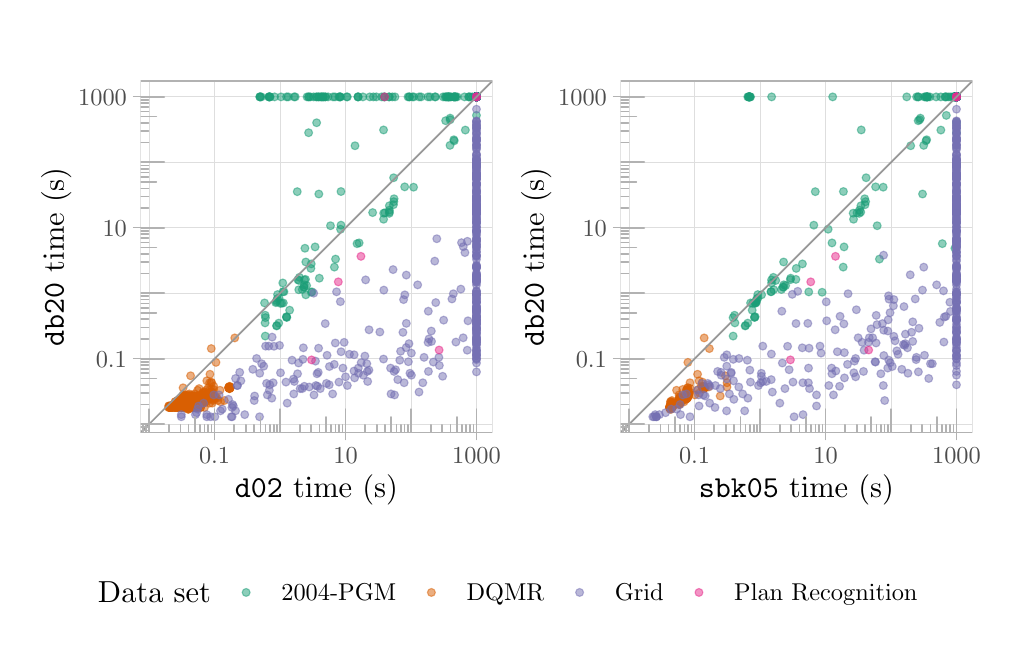
\begin{tikzpicture}[x=1pt,y=1pt]
\definecolor{fillColor}{RGB}{255,255,255}
\path[use as bounding box,fill=fillColor,fill opacity=0.00] (0,0) rectangle (346.90,216.81);
\begin{scope}
\path[clip] (  0.00, 39.18) rectangle (173.45,203.08);
\definecolor{drawColor}{RGB}{255,255,255}
\definecolor{fillColor}{RGB}{255,255,255}

\path[draw=drawColor,line width= 0.6pt,line join=round,line cap=round,fill=fillColor] (  0.00, 39.18) rectangle (173.45,203.08);
\end{scope}
\begin{scope}
\path[clip] ( 40.80, 70.44) rectangle (167.95,197.58);
\definecolor{fillColor}{RGB}{255,255,255}

\path[fill=fillColor] ( 40.80, 70.44) rectangle (167.95,197.58);
\definecolor{drawColor}{gray}{0.87}

\path[draw=drawColor,line width= 0.1pt,line join=round] ( 40.80, 73.52) --
	(167.95, 73.52);

\path[draw=drawColor,line width= 0.1pt,line join=round] ( 40.80,120.83) --
	(167.95,120.83);

\path[draw=drawColor,line width= 0.1pt,line join=round] ( 40.80,168.15) --
	(167.95,168.15);

\path[draw=drawColor,line width= 0.1pt,line join=round] ( 43.88, 70.44) --
	( 43.88,197.58);

\path[draw=drawColor,line width= 0.1pt,line join=round] ( 91.20, 70.44) --
	( 91.20,197.58);

\path[draw=drawColor,line width= 0.1pt,line join=round] (138.51, 70.44) --
	(138.51,197.58);

\path[draw=drawColor,line width= 0.3pt,line join=round] ( 40.80, 97.18) --
	(167.95, 97.18);

\path[draw=drawColor,line width= 0.3pt,line join=round] ( 40.80,144.49) --
	(167.95,144.49);

\path[draw=drawColor,line width= 0.3pt,line join=round] ( 40.80,191.80) --
	(167.95,191.80);

\path[draw=drawColor,line width= 0.3pt,line join=round] ( 67.54, 70.44) --
	( 67.54,197.58);

\path[draw=drawColor,line width= 0.3pt,line join=round] (114.86, 70.44) --
	(114.86,197.58);

\path[draw=drawColor,line width= 0.3pt,line join=round] (162.17, 70.44) --
	(162.17,197.58);
\definecolor{drawColor}{RGB}{27,158,119}
\definecolor{fillColor}{RGB}{27,158,119}

\path[draw=drawColor,draw opacity=0.50,line width= 0.4pt,line join=round,line cap=round,fill=fillColor,fill opacity=0.50] ( 87.58,191.80) circle (  1.43);

\path[draw=drawColor,draw opacity=0.50,line width= 0.4pt,line join=round,line cap=round,fill=fillColor,fill opacity=0.50] ( 87.16,191.80) circle (  1.43);

\path[draw=drawColor,draw opacity=0.50,line width= 0.4pt,line join=round,line cap=round,fill=fillColor,fill opacity=0.50] ( 87.36,191.80) circle (  1.43);

\path[draw=drawColor,draw opacity=0.50,line width= 0.4pt,line join=round,line cap=round,fill=fillColor,fill opacity=0.50] ( 89.22,191.80) circle (  1.43);

\path[draw=drawColor,draw opacity=0.50,line width= 0.4pt,line join=round,line cap=round,fill=fillColor,fill opacity=0.50] ( 87.16,191.80) circle (  1.43);

\path[draw=drawColor,draw opacity=0.50,line width= 0.4pt,line join=round,line cap=round,fill=fillColor,fill opacity=0.50] ( 87.53,191.80) circle (  1.43);

\path[draw=drawColor,draw opacity=0.50,line width= 0.4pt,line join=round,line cap=round,fill=fillColor,fill opacity=0.50] ( 85.83,112.90) circle (  1.43);

\path[draw=drawColor,draw opacity=0.50,line width= 0.4pt,line join=round,line cap=round,fill=fillColor,fill opacity=0.50] ( 85.93,112.04) circle (  1.43);

\path[draw=drawColor,draw opacity=0.50,line width= 0.4pt,line join=round,line cap=round,fill=fillColor,fill opacity=0.50] ( 85.85,105.37) circle (  1.43);

\path[draw=drawColor,draw opacity=0.50,line width= 0.4pt,line join=round,line cap=round,fill=fillColor,fill opacity=0.50] ( 94.66,114.73) circle (  1.43);

\path[draw=drawColor,draw opacity=0.50,line width= 0.4pt,line join=round,line cap=round,fill=fillColor,fill opacity=0.50] ( 85.79,110.13) circle (  1.43);

\path[draw=drawColor,draw opacity=0.50,line width= 0.4pt,line join=round,line cap=round,fill=fillColor,fill opacity=0.50] ( 84.44,191.80) circle (  1.43);

\path[draw=drawColor,draw opacity=0.50,line width= 0.4pt,line join=round,line cap=round,fill=fillColor,fill opacity=0.50] ( 83.89,191.80) circle (  1.43);

\path[draw=drawColor,draw opacity=0.50,line width= 0.4pt,line join=round,line cap=round,fill=fillColor,fill opacity=0.50] ( 94.17,191.80) circle (  1.43);

\path[draw=drawColor,draw opacity=0.50,line width= 0.4pt,line join=round,line cap=round,fill=fillColor,fill opacity=0.50] ( 83.95,191.80) circle (  1.43);

\path[draw=drawColor,draw opacity=0.50,line width= 0.4pt,line join=round,line cap=round,fill=fillColor,fill opacity=0.50] ( 83.99,191.80) circle (  1.43);

\path[draw=drawColor,draw opacity=0.50,line width= 0.4pt,line join=round,line cap=round,fill=fillColor,fill opacity=0.50] ( 90.30,120.37) circle (  1.43);

\path[draw=drawColor,draw opacity=0.50,line width= 0.4pt,line join=round,line cap=round,fill=fillColor,fill opacity=0.50] ( 89.65,117.47) circle (  1.43);

\path[draw=drawColor,draw opacity=0.50,line width= 0.4pt,line join=round,line cap=round,fill=fillColor,fill opacity=0.50] ( 90.00,118.21) circle (  1.43);

\path[draw=drawColor,draw opacity=0.50,line width= 0.4pt,line join=round,line cap=round,fill=fillColor,fill opacity=0.50] ( 98.04,125.45) circle (  1.43);

\path[draw=drawColor,draw opacity=0.50,line width= 0.4pt,line join=round,line cap=round,fill=fillColor,fill opacity=0.50] ( 89.93,117.73) circle (  1.43);

\path[draw=drawColor,draw opacity=0.50,line width= 0.4pt,line join=round,line cap=round,fill=fillColor,fill opacity=0.50] ( 90.82,119.15) circle (  1.43);

\path[draw=drawColor,draw opacity=0.50,line width= 0.4pt,line join=round,line cap=round,fill=fillColor,fill opacity=0.50] (100.51,120.28) circle (  1.43);

\path[draw=drawColor,draw opacity=0.50,line width= 0.4pt,line join=round,line cap=round,fill=fillColor,fill opacity=0.50] ( 90.02,109.16) circle (  1.43);

\path[draw=drawColor,draw opacity=0.50,line width= 0.4pt,line join=round,line cap=round,fill=fillColor,fill opacity=0.50] ( 90.73,110.05) circle (  1.43);

\path[draw=drawColor,draw opacity=0.50,line width= 0.4pt,line join=round,line cap=round,fill=fillColor,fill opacity=0.50] ( 89.94,109.03) circle (  1.43);

\path[draw=drawColor,draw opacity=0.50,line width= 0.4pt,line join=round,line cap=round,fill=fillColor,fill opacity=0.50] ( 85.60,117.34) circle (  1.43);

\path[draw=drawColor,draw opacity=0.50,line width= 0.4pt,line join=round,line cap=round,fill=fillColor,fill opacity=0.50] ( 92.38,117.34) circle (  1.43);

\path[draw=drawColor,draw opacity=0.50,line width= 0.4pt,line join=round,line cap=round,fill=fillColor,fill opacity=0.50] ( 99.98,125.66) circle (  1.43);

\path[draw=drawColor,draw opacity=0.50,line width= 0.4pt,line join=round,line cap=round,fill=fillColor,fill opacity=0.50] ( 91.83,117.27) circle (  1.43);

\path[draw=drawColor,draw opacity=0.50,line width= 0.4pt,line join=round,line cap=round,fill=fillColor,fill opacity=0.50] ( 98.21,126.59) circle (  1.43);

\path[draw=drawColor,draw opacity=0.50,line width= 0.4pt,line join=round,line cap=round,fill=fillColor,fill opacity=0.50] ( 91.33,117.18) circle (  1.43);

\path[draw=drawColor,draw opacity=0.50,line width= 0.4pt,line join=round,line cap=round,fill=fillColor,fill opacity=0.50] ( 99.91,123.05) circle (  1.43);

\path[draw=drawColor,draw opacity=0.50,line width= 0.4pt,line join=round,line cap=round,fill=fillColor,fill opacity=0.50] ( 99.78,123.06) circle (  1.43);

\path[draw=drawColor,draw opacity=0.50,line width= 0.4pt,line join=round,line cap=round,fill=fillColor,fill opacity=0.50] (102.47,131.45) circle (  1.43);

\path[draw=drawColor,draw opacity=0.50,line width= 0.4pt,line join=round,line cap=round,fill=fillColor,fill opacity=0.50] ( 99.24,122.20) circle (  1.43);

\path[draw=drawColor,draw opacity=0.50,line width= 0.4pt,line join=round,line cap=round,fill=fillColor,fill opacity=0.50] ( 99.95,123.90) circle (  1.43);

\path[draw=drawColor,draw opacity=0.50,line width= 0.4pt,line join=round,line cap=round,fill=fillColor,fill opacity=0.50] (100.80,123.61) circle (  1.43);

\path[draw=drawColor,draw opacity=0.50,line width= 0.4pt,line join=round,line cap=round,fill=fillColor,fill opacity=0.50] ( 93.53,112.23) circle (  1.43);

\path[draw=drawColor,draw opacity=0.50,line width= 0.4pt,line join=round,line cap=round,fill=fillColor,fill opacity=0.50] ( 90.21,118.87) circle (  1.43);

\path[draw=drawColor,draw opacity=0.50,line width= 0.4pt,line join=round,line cap=round,fill=fillColor,fill opacity=0.50] (105.39,126.28) circle (  1.43);

\path[draw=drawColor,draw opacity=0.50,line width= 0.4pt,line join=round,line cap=round,fill=fillColor,fill opacity=0.50] ( 93.52,112.37) circle (  1.43);

\path[draw=drawColor,draw opacity=0.50,line width= 0.4pt,line join=round,line cap=round,fill=fillColor,fill opacity=0.50] ( 93.63,112.09) circle (  1.43);

\path[draw=drawColor,draw opacity=0.50,line width= 0.4pt,line join=round,line cap=round,fill=fillColor,fill opacity=0.50] (102.33,129.82) circle (  1.43);

\path[draw=drawColor,draw opacity=0.50,line width= 0.4pt,line join=round,line cap=round,fill=fillColor,fill opacity=0.50] ( 92.25,121.42) circle (  1.43);

\path[draw=drawColor,draw opacity=0.50,line width= 0.4pt,line join=round,line cap=round,fill=fillColor,fill opacity=0.50] ( 92.61,121.38) circle (  1.43);

\path[draw=drawColor,draw opacity=0.50,line width= 0.4pt,line join=round,line cap=round,fill=fillColor,fill opacity=0.50] ( 92.18,124.56) circle (  1.43);

\path[draw=drawColor,draw opacity=0.50,line width= 0.4pt,line join=round,line cap=round,fill=fillColor,fill opacity=0.50] ( 97.96,122.11) circle (  1.43);

\path[draw=drawColor,draw opacity=0.50,line width= 0.4pt,line join=round,line cap=round,fill=fillColor,fill opacity=0.50] (162.17,191.80) circle (  1.43);

\path[draw=drawColor,draw opacity=0.50,line width= 0.4pt,line join=round,line cap=round,fill=fillColor,fill opacity=0.50] (128.98,191.80) circle (  1.43);

\path[draw=drawColor,draw opacity=0.50,line width= 0.4pt,line join=round,line cap=round,fill=fillColor,fill opacity=0.50] (137.43,191.80) circle (  1.43);

\path[draw=drawColor,draw opacity=0.50,line width= 0.4pt,line join=round,line cap=round,fill=fillColor,fill opacity=0.50] (162.17,191.80) circle (  1.43);

\path[draw=drawColor,draw opacity=0.50,line width= 0.4pt,line join=round,line cap=round,fill=fillColor,fill opacity=0.50] (128.80,191.80) circle (  1.43);

\path[draw=drawColor,draw opacity=0.50,line width= 0.4pt,line join=round,line cap=round,fill=fillColor,fill opacity=0.50] (162.17,191.80) circle (  1.43);

\path[draw=drawColor,draw opacity=0.50,line width= 0.4pt,line join=round,line cap=round,fill=fillColor,fill opacity=0.50] (128.60,179.85) circle (  1.43);

\path[draw=drawColor,draw opacity=0.50,line width= 0.4pt,line join=round,line cap=round,fill=fillColor,fill opacity=0.50] (136.23,159.29) circle (  1.43);

\path[draw=drawColor,draw opacity=0.50,line width= 0.4pt,line join=round,line cap=round,fill=fillColor,fill opacity=0.50] (128.60,147.58) circle (  1.43);

\path[draw=drawColor,draw opacity=0.50,line width= 0.4pt,line join=round,line cap=round,fill=fillColor,fill opacity=0.50] (129.11,149.92) circle (  1.43);

\path[draw=drawColor,draw opacity=0.50,line width= 0.4pt,line join=round,line cap=round,fill=fillColor,fill opacity=0.50] (128.65,149.77) circle (  1.43);

\path[draw=drawColor,draw opacity=0.50,line width= 0.4pt,line join=round,line cap=round,fill=fillColor,fill opacity=0.50] (147.37,191.80) circle (  1.43);

\path[draw=drawColor,draw opacity=0.50,line width= 0.4pt,line join=round,line cap=round,fill=fillColor,fill opacity=0.50] (162.17,191.80) circle (  1.43);

\path[draw=drawColor,draw opacity=0.50,line width= 0.4pt,line join=round,line cap=round,fill=fillColor,fill opacity=0.50] (141.45,191.80) circle (  1.43);

\path[draw=drawColor,draw opacity=0.50,line width= 0.4pt,line join=round,line cap=round,fill=fillColor,fill opacity=0.50] (152.49,191.80) circle (  1.43);

\path[draw=drawColor,draw opacity=0.50,line width= 0.4pt,line join=round,line cap=round,fill=fillColor,fill opacity=0.50] (145.40,191.80) circle (  1.43);

\path[draw=drawColor,draw opacity=0.50,line width= 0.4pt,line join=round,line cap=round,fill=fillColor,fill opacity=0.50] (162.17,191.80) circle (  1.43);

\path[draw=drawColor,draw opacity=0.50,line width= 0.4pt,line join=round,line cap=round,fill=fillColor,fill opacity=0.50] (139.52,191.80) circle (  1.43);

\path[draw=drawColor,draw opacity=0.50,line width= 0.4pt,line join=round,line cap=round,fill=fillColor,fill opacity=0.50] (130.51,191.80) circle (  1.43);

\path[draw=drawColor,draw opacity=0.50,line width= 0.4pt,line join=round,line cap=round,fill=fillColor,fill opacity=0.50] (162.17,191.80) circle (  1.43);

\path[draw=drawColor,draw opacity=0.50,line width= 0.4pt,line join=round,line cap=round,fill=fillColor,fill opacity=0.50] (162.17,191.80) circle (  1.43);

\path[draw=drawColor,draw opacity=0.50,line width= 0.4pt,line join=round,line cap=round,fill=fillColor,fill opacity=0.50] (162.17,191.80) circle (  1.43);

\path[draw=drawColor,draw opacity=0.50,line width= 0.4pt,line join=round,line cap=round,fill=fillColor,fill opacity=0.50] (139.44,159.17) circle (  1.43);

\path[draw=drawColor,draw opacity=0.50,line width= 0.4pt,line join=round,line cap=round,fill=fillColor,fill opacity=0.50] (130.69,150.87) circle (  1.43);

\path[draw=drawColor,draw opacity=0.50,line width= 0.4pt,line join=round,line cap=round,fill=fillColor,fill opacity=0.50] (130.73,150.19) circle (  1.43);

\path[draw=drawColor,draw opacity=0.50,line width= 0.4pt,line join=round,line cap=round,fill=fillColor,fill opacity=0.50] (130.70,152.45) circle (  1.43);

\path[draw=drawColor,draw opacity=0.50,line width= 0.4pt,line join=round,line cap=round,fill=fillColor,fill opacity=0.50] (130.66,149.71) circle (  1.43);

\path[draw=drawColor,draw opacity=0.50,line width= 0.4pt,line join=round,line cap=round,fill=fillColor,fill opacity=0.50] (162.17,191.80) circle (  1.43);

\path[draw=drawColor,draw opacity=0.50,line width= 0.4pt,line join=round,line cap=round,fill=fillColor,fill opacity=0.50] (159.94,191.80) circle (  1.43);

\path[draw=drawColor,draw opacity=0.50,line width= 0.4pt,line join=round,line cap=round,fill=fillColor,fill opacity=0.50] (142.16,191.80) circle (  1.43);

\path[draw=drawColor,draw opacity=0.50,line width= 0.4pt,line join=round,line cap=round,fill=fillColor,fill opacity=0.50] (159.50,191.80) circle (  1.43);

\path[draw=drawColor,draw opacity=0.50,line width= 0.4pt,line join=round,line cap=round,fill=fillColor,fill opacity=0.50] (157.85,191.80) circle (  1.43);

\path[draw=drawColor,draw opacity=0.50,line width= 0.4pt,line join=round,line cap=round,fill=fillColor,fill opacity=0.50] (162.17,191.80) circle (  1.43);

\path[draw=drawColor,draw opacity=0.50,line width= 0.4pt,line join=round,line cap=round,fill=fillColor,fill opacity=0.50] (162.17,191.80) circle (  1.43);

\path[draw=drawColor,draw opacity=0.50,line width= 0.4pt,line join=round,line cap=round,fill=fillColor,fill opacity=0.50] (162.17,191.80) circle (  1.43);

\path[draw=drawColor,draw opacity=0.50,line width= 0.4pt,line join=round,line cap=round,fill=fillColor,fill opacity=0.50] (162.17,191.80) circle (  1.43);

\path[draw=drawColor,draw opacity=0.50,line width= 0.4pt,line join=round,line cap=round,fill=fillColor,fill opacity=0.50] (162.17,191.80) circle (  1.43);

\path[draw=drawColor,draw opacity=0.50,line width= 0.4pt,line join=round,line cap=round,fill=fillColor,fill opacity=0.50] (162.17,191.80) circle (  1.43);

\path[draw=drawColor,draw opacity=0.50,line width= 0.4pt,line join=round,line cap=round,fill=fillColor,fill opacity=0.50] (162.17,191.80) circle (  1.43);

\path[draw=drawColor,draw opacity=0.50,line width= 0.4pt,line join=round,line cap=round,fill=fillColor,fill opacity=0.50] (132.39,154.99) circle (  1.43);

\path[draw=drawColor,draw opacity=0.50,line width= 0.4pt,line join=round,line cap=round,fill=fillColor,fill opacity=0.50] (132.23,162.58) circle (  1.43);

\path[draw=drawColor,draw opacity=0.50,line width= 0.4pt,line join=round,line cap=round,fill=fillColor,fill opacity=0.50] (132.30,153.93) circle (  1.43);

\path[draw=drawColor,draw opacity=0.50,line width= 0.4pt,line join=round,line cap=round,fill=fillColor,fill opacity=0.50] (132.16,152.83) circle (  1.43);

\path[draw=drawColor,draw opacity=0.50,line width= 0.4pt,line join=round,line cap=round,fill=fillColor,fill opacity=0.50] (162.17,191.80) circle (  1.43);

\path[draw=drawColor,draw opacity=0.50,line width= 0.4pt,line join=round,line cap=round,fill=fillColor,fill opacity=0.50] (162.17,191.80) circle (  1.43);

\path[draw=drawColor,draw opacity=0.50,line width= 0.4pt,line join=round,line cap=round,fill=fillColor,fill opacity=0.50] (162.17,191.80) circle (  1.43);

\path[draw=drawColor,draw opacity=0.50,line width= 0.4pt,line join=round,line cap=round,fill=fillColor,fill opacity=0.50] (162.03,191.80) circle (  1.43);

\path[draw=drawColor,draw opacity=0.50,line width= 0.4pt,line join=round,line cap=round,fill=fillColor,fill opacity=0.50] (162.17,191.80) circle (  1.43);

\path[draw=drawColor,draw opacity=0.50,line width= 0.4pt,line join=round,line cap=round,fill=fillColor,fill opacity=0.50] (162.17,191.80) circle (  1.43);

\path[draw=drawColor,draw opacity=0.50,line width= 0.4pt,line join=round,line cap=round,fill=fillColor,fill opacity=0.50] (161.96,191.80) circle (  1.43);

\path[draw=drawColor,draw opacity=0.50,line width= 0.4pt,line join=round,line cap=round,fill=fillColor,fill opacity=0.50] (162.12,191.80) circle (  1.43);

\path[draw=drawColor,draw opacity=0.50,line width= 0.4pt,line join=round,line cap=round,fill=fillColor,fill opacity=0.50] (162.17,191.80) circle (  1.43);

\path[draw=drawColor,draw opacity=0.50,line width= 0.4pt,line join=round,line cap=round,fill=fillColor,fill opacity=0.50] (162.06,191.80) circle (  1.43);

\path[draw=drawColor,draw opacity=0.50,line width= 0.4pt,line join=round,line cap=round,fill=fillColor,fill opacity=0.50] (162.17,191.80) circle (  1.43);

\path[draw=drawColor,draw opacity=0.50,line width= 0.4pt,line join=round,line cap=round,fill=fillColor,fill opacity=0.50] (151.21,191.80) circle (  1.43);

\path[draw=drawColor,draw opacity=0.50,line width= 0.4pt,line join=round,line cap=round,fill=fillColor,fill opacity=0.50] (151.03,183.19) circle (  1.43);

\path[draw=drawColor,draw opacity=0.50,line width= 0.4pt,line join=round,line cap=round,fill=fillColor,fill opacity=0.50] (151.34,191.80) circle (  1.43);

\path[draw=drawColor,draw opacity=0.50,line width= 0.4pt,line join=round,line cap=round,fill=fillColor,fill opacity=0.50] (147.15,191.80) circle (  1.43);

\path[draw=drawColor,draw opacity=0.50,line width= 0.4pt,line join=round,line cap=round,fill=fillColor,fill opacity=0.50] (160.77,191.80) circle (  1.43);

\path[draw=drawColor,draw opacity=0.50,line width= 0.4pt,line join=round,line cap=round,fill=fillColor,fill opacity=0.50] (152.57,191.80) circle (  1.43);

\path[draw=drawColor,draw opacity=0.50,line width= 0.4pt,line join=round,line cap=round,fill=fillColor,fill opacity=0.50] (162.17,191.80) circle (  1.43);

\path[draw=drawColor,draw opacity=0.50,line width= 0.4pt,line join=round,line cap=round,fill=fillColor,fill opacity=0.50] (154.41,191.80) circle (  1.43);

\path[draw=drawColor,draw opacity=0.50,line width= 0.4pt,line join=round,line cap=round,fill=fillColor,fill opacity=0.50] (159.35,191.80) circle (  1.43);

\path[draw=drawColor,draw opacity=0.50,line width= 0.4pt,line join=round,line cap=round,fill=fillColor,fill opacity=0.50] (154.58,191.80) circle (  1.43);

\path[draw=drawColor,draw opacity=0.50,line width= 0.4pt,line join=round,line cap=round,fill=fillColor,fill opacity=0.50] (162.17,191.80) circle (  1.43);

\path[draw=drawColor,draw opacity=0.50,line width= 0.4pt,line join=round,line cap=round,fill=fillColor,fill opacity=0.50] (162.17,191.80) circle (  1.43);

\path[draw=drawColor,draw opacity=0.50,line width= 0.4pt,line join=round,line cap=round,fill=fillColor,fill opacity=0.50] (162.17,191.80) circle (  1.43);

\path[draw=drawColor,draw opacity=0.50,line width= 0.4pt,line join=round,line cap=round,fill=fillColor,fill opacity=0.50] (162.17,191.80) circle (  1.43);

\path[draw=drawColor,draw opacity=0.50,line width= 0.4pt,line join=round,line cap=round,fill=fillColor,fill opacity=0.50] (162.17,191.80) circle (  1.43);

\path[draw=drawColor,draw opacity=0.50,line width= 0.4pt,line join=round,line cap=round,fill=fillColor,fill opacity=0.50] (162.17,191.80) circle (  1.43);

\path[draw=drawColor,draw opacity=0.50,line width= 0.4pt,line join=round,line cap=round,fill=fillColor,fill opacity=0.50] (152.60,174.28) circle (  1.43);

\path[draw=drawColor,draw opacity=0.50,line width= 0.4pt,line join=round,line cap=round,fill=fillColor,fill opacity=0.50] (152.66,184.12) circle (  1.43);

\path[draw=drawColor,draw opacity=0.50,line width= 0.4pt,line join=round,line cap=round,fill=fillColor,fill opacity=0.50] (158.15,179.81) circle (  1.43);

\path[draw=drawColor,draw opacity=0.50,line width= 0.4pt,line join=round,line cap=round,fill=fillColor,fill opacity=0.50] (152.64,183.53) circle (  1.43);

\path[draw=drawColor,draw opacity=0.50,line width= 0.4pt,line join=round,line cap=round,fill=fillColor,fill opacity=0.50] (155.19,191.80) circle (  1.43);

\path[draw=drawColor,draw opacity=0.50,line width= 0.4pt,line join=round,line cap=round,fill=fillColor,fill opacity=0.50] (150.85,191.80) circle (  1.43);

\path[draw=drawColor,draw opacity=0.50,line width= 0.4pt,line join=round,line cap=round,fill=fillColor,fill opacity=0.50] (150.12,191.80) circle (  1.43);

\path[draw=drawColor,draw opacity=0.50,line width= 0.4pt,line join=round,line cap=round,fill=fillColor,fill opacity=0.50] (153.00,191.80) circle (  1.43);

\path[draw=drawColor,draw opacity=0.50,line width= 0.4pt,line join=round,line cap=round,fill=fillColor,fill opacity=0.50] (152.03,191.80) circle (  1.43);

\path[draw=drawColor,draw opacity=0.50,line width= 0.4pt,line join=round,line cap=round,fill=fillColor,fill opacity=0.50] (152.01,191.80) circle (  1.43);

\path[draw=drawColor,draw opacity=0.50,line width= 0.4pt,line join=round,line cap=round,fill=fillColor,fill opacity=0.50] (162.17,191.80) circle (  1.43);

\path[draw=drawColor,draw opacity=0.50,line width= 0.4pt,line join=round,line cap=round,fill=fillColor,fill opacity=0.50] (162.17,191.80) circle (  1.43);

\path[draw=drawColor,draw opacity=0.50,line width= 0.4pt,line join=round,line cap=round,fill=fillColor,fill opacity=0.50] (162.17,191.80) circle (  1.43);

\path[draw=drawColor,draw opacity=0.50,line width= 0.4pt,line join=round,line cap=round,fill=fillColor,fill opacity=0.50] (162.17,191.80) circle (  1.43);

\path[draw=drawColor,draw opacity=0.50,line width= 0.4pt,line join=round,line cap=round,fill=fillColor,fill opacity=0.50] (162.17,191.80) circle (  1.43);

\path[draw=drawColor,draw opacity=0.50,line width= 0.4pt,line join=round,line cap=round,fill=fillColor,fill opacity=0.50] (162.17,191.80) circle (  1.43);

\path[draw=drawColor,draw opacity=0.50,line width= 0.4pt,line join=round,line cap=round,fill=fillColor,fill opacity=0.50] (162.17,191.80) circle (  1.43);

\path[draw=drawColor,draw opacity=0.50,line width= 0.4pt,line join=round,line cap=round,fill=fillColor,fill opacity=0.50] (154.11,191.80) circle (  1.43);

\path[draw=drawColor,draw opacity=0.50,line width= 0.4pt,line join=round,line cap=round,fill=fillColor,fill opacity=0.50] (162.17,185.11) circle (  1.43);

\path[draw=drawColor,draw opacity=0.50,line width= 0.4pt,line join=round,line cap=round,fill=fillColor,fill opacity=0.50] (153.98,176.31) circle (  1.43);

\path[draw=drawColor,draw opacity=0.50,line width= 0.4pt,line join=round,line cap=round,fill=fillColor,fill opacity=0.50] (154.13,175.92) circle (  1.43);

\path[draw=drawColor,draw opacity=0.50,line width= 0.4pt,line join=round,line cap=round,fill=fillColor,fill opacity=0.50] (151.87,191.80) circle (  1.43);

\path[draw=drawColor,draw opacity=0.50,line width= 0.4pt,line join=round,line cap=round,fill=fillColor,fill opacity=0.50] (153.89,191.80) circle (  1.43);

\path[draw=drawColor,draw opacity=0.50,line width= 0.4pt,line join=round,line cap=round,fill=fillColor,fill opacity=0.50] (151.90,191.80) circle (  1.43);

\path[draw=drawColor,draw opacity=0.50,line width= 0.4pt,line join=round,line cap=round,fill=fillColor,fill opacity=0.50] (154.59,191.80) circle (  1.43);

\path[draw=drawColor,draw opacity=0.50,line width= 0.4pt,line join=round,line cap=round,fill=fillColor,fill opacity=0.50] (154.10,191.80) circle (  1.43);

\path[draw=drawColor,draw opacity=0.50,line width= 0.4pt,line join=round,line cap=round,fill=fillColor,fill opacity=0.50] (162.17,191.80) circle (  1.43);

\path[draw=drawColor,draw opacity=0.50,line width= 0.4pt,line join=round,line cap=round,fill=fillColor,fill opacity=0.50] (162.17,191.80) circle (  1.43);

\path[draw=drawColor,draw opacity=0.50,line width= 0.4pt,line join=round,line cap=round,fill=fillColor,fill opacity=0.50] (162.17,191.80) circle (  1.43);

\path[draw=drawColor,draw opacity=0.50,line width= 0.4pt,line join=round,line cap=round,fill=fillColor,fill opacity=0.50] (162.17,191.80) circle (  1.43);

\path[draw=drawColor,draw opacity=0.50,line width= 0.4pt,line join=round,line cap=round,fill=fillColor,fill opacity=0.50] (162.17,191.80) circle (  1.43);

\path[draw=drawColor,draw opacity=0.50,line width= 0.4pt,line join=round,line cap=round,fill=fillColor,fill opacity=0.50] (162.17,191.80) circle (  1.43);

\path[draw=drawColor,draw opacity=0.50,line width= 0.4pt,line join=round,line cap=round,fill=fillColor,fill opacity=0.50] (162.17,191.80) circle (  1.43);

\path[draw=drawColor,draw opacity=0.50,line width= 0.4pt,line join=round,line cap=round,fill=fillColor,fill opacity=0.50] (162.17,191.80) circle (  1.43);

\path[draw=drawColor,draw opacity=0.50,line width= 0.4pt,line join=round,line cap=round,fill=fillColor,fill opacity=0.50] (162.17,191.80) circle (  1.43);

\path[draw=drawColor,draw opacity=0.50,line width= 0.4pt,line join=round,line cap=round,fill=fillColor,fill opacity=0.50] (162.17,191.80) circle (  1.43);

\path[draw=drawColor,draw opacity=0.50,line width= 0.4pt,line join=round,line cap=round,fill=fillColor,fill opacity=0.50] (162.17,191.80) circle (  1.43);

\path[draw=drawColor,draw opacity=0.50,line width= 0.4pt,line join=round,line cap=round,fill=fillColor,fill opacity=0.50] (162.17,191.80) circle (  1.43);

\path[draw=drawColor,draw opacity=0.50,line width= 0.4pt,line join=round,line cap=round,fill=fillColor,fill opacity=0.50] (162.17,191.80) circle (  1.43);

\path[draw=drawColor,draw opacity=0.50,line width= 0.4pt,line join=round,line cap=round,fill=fillColor,fill opacity=0.50] (162.17,191.80) circle (  1.43);

\path[draw=drawColor,draw opacity=0.50,line width= 0.4pt,line join=round,line cap=round,fill=fillColor,fill opacity=0.50] (162.17,191.80) circle (  1.43);

\path[draw=drawColor,draw opacity=0.50,line width= 0.4pt,line join=round,line cap=round,fill=fillColor,fill opacity=0.50] (162.17,191.80) circle (  1.43);

\path[draw=drawColor,draw opacity=0.50,line width= 0.4pt,line join=round,line cap=round,fill=fillColor,fill opacity=0.50] (162.17,191.80) circle (  1.43);

\path[draw=drawColor,draw opacity=0.50,line width= 0.4pt,line join=round,line cap=round,fill=fillColor,fill opacity=0.50] (162.17,191.80) circle (  1.43);

\path[draw=drawColor,draw opacity=0.50,line width= 0.4pt,line join=round,line cap=round,fill=fillColor,fill opacity=0.50] (162.17,191.80) circle (  1.43);

\path[draw=drawColor,draw opacity=0.50,line width= 0.4pt,line join=round,line cap=round,fill=fillColor,fill opacity=0.50] (162.17,191.80) circle (  1.43);

\path[draw=drawColor,draw opacity=0.50,line width= 0.4pt,line join=round,line cap=round,fill=fillColor,fill opacity=0.50] (162.17,191.80) circle (  1.43);

\path[draw=drawColor,draw opacity=0.50,line width= 0.4pt,line join=round,line cap=round,fill=fillColor,fill opacity=0.50] (162.17,191.80) circle (  1.43);

\path[draw=drawColor,draw opacity=0.50,line width= 0.4pt,line join=round,line cap=round,fill=fillColor,fill opacity=0.50] (162.17,191.80) circle (  1.43);

\path[draw=drawColor,draw opacity=0.50,line width= 0.4pt,line join=round,line cap=round,fill=fillColor,fill opacity=0.50] (162.17,191.80) circle (  1.43);

\path[draw=drawColor,draw opacity=0.50,line width= 0.4pt,line join=round,line cap=round,fill=fillColor,fill opacity=0.50] (162.17,191.80) circle (  1.43);

\path[draw=drawColor,draw opacity=0.50,line width= 0.4pt,line join=round,line cap=round,fill=fillColor,fill opacity=0.50] (162.17,191.80) circle (  1.43);

\path[draw=drawColor,draw opacity=0.50,line width= 0.4pt,line join=round,line cap=round,fill=fillColor,fill opacity=0.50] (162.17,191.80) circle (  1.43);

\path[draw=drawColor,draw opacity=0.50,line width= 0.4pt,line join=round,line cap=round,fill=fillColor,fill opacity=0.50] (162.17,191.80) circle (  1.43);

\path[draw=drawColor,draw opacity=0.50,line width= 0.4pt,line join=round,line cap=round,fill=fillColor,fill opacity=0.50] (162.17,191.80) circle (  1.43);

\path[draw=drawColor,draw opacity=0.50,line width= 0.4pt,line join=round,line cap=round,fill=fillColor,fill opacity=0.50] (162.17,191.80) circle (  1.43);

\path[draw=drawColor,draw opacity=0.50,line width= 0.4pt,line join=round,line cap=round,fill=fillColor,fill opacity=0.50] (162.17,191.80) circle (  1.43);

\path[draw=drawColor,draw opacity=0.50,line width= 0.4pt,line join=round,line cap=round,fill=fillColor,fill opacity=0.50] (162.17,191.80) circle (  1.43);

\path[draw=drawColor,draw opacity=0.50,line width= 0.4pt,line join=round,line cap=round,fill=fillColor,fill opacity=0.50] (162.17,191.80) circle (  1.43);

\path[draw=drawColor,draw opacity=0.50,line width= 0.4pt,line join=round,line cap=round,fill=fillColor,fill opacity=0.50] (162.17,191.80) circle (  1.43);

\path[draw=drawColor,draw opacity=0.50,line width= 0.4pt,line join=round,line cap=round,fill=fillColor,fill opacity=0.50] (162.17,191.80) circle (  1.43);

\path[draw=drawColor,draw opacity=0.50,line width= 0.4pt,line join=round,line cap=round,fill=fillColor,fill opacity=0.50] (162.17,191.80) circle (  1.43);

\path[draw=drawColor,draw opacity=0.50,line width= 0.4pt,line join=round,line cap=round,fill=fillColor,fill opacity=0.50] (162.17,191.80) circle (  1.43);

\path[draw=drawColor,draw opacity=0.50,line width= 0.4pt,line join=round,line cap=round,fill=fillColor,fill opacity=0.50] (162.17,191.80) circle (  1.43);

\path[draw=drawColor,draw opacity=0.50,line width= 0.4pt,line join=round,line cap=round,fill=fillColor,fill opacity=0.50] (162.17,191.80) circle (  1.43);

\path[draw=drawColor,draw opacity=0.50,line width= 0.4pt,line join=round,line cap=round,fill=fillColor,fill opacity=0.50] (162.17,191.80) circle (  1.43);

\path[draw=drawColor,draw opacity=0.50,line width= 0.4pt,line join=round,line cap=round,fill=fillColor,fill opacity=0.50] (162.17,191.80) circle (  1.43);

\path[draw=drawColor,draw opacity=0.50,line width= 0.4pt,line join=round,line cap=round,fill=fillColor,fill opacity=0.50] (162.17,191.80) circle (  1.43);

\path[draw=drawColor,draw opacity=0.50,line width= 0.4pt,line join=round,line cap=round,fill=fillColor,fill opacity=0.50] (162.17,191.80) circle (  1.43);

\path[draw=drawColor,draw opacity=0.50,line width= 0.4pt,line join=round,line cap=round,fill=fillColor,fill opacity=0.50] (162.17,191.80) circle (  1.43);

\path[draw=drawColor,draw opacity=0.50,line width= 0.4pt,line join=round,line cap=round,fill=fillColor,fill opacity=0.50] (162.17,191.80) circle (  1.43);

\path[draw=drawColor,draw opacity=0.50,line width= 0.4pt,line join=round,line cap=round,fill=fillColor,fill opacity=0.50] (162.17,191.80) circle (  1.43);

\path[draw=drawColor,draw opacity=0.50,line width= 0.4pt,line join=round,line cap=round,fill=fillColor,fill opacity=0.50] (162.17,191.80) circle (  1.43);

\path[draw=drawColor,draw opacity=0.50,line width= 0.4pt,line join=round,line cap=round,fill=fillColor,fill opacity=0.50] (162.17,191.80) circle (  1.43);

\path[draw=drawColor,draw opacity=0.50,line width= 0.4pt,line join=round,line cap=round,fill=fillColor,fill opacity=0.50] (162.17,191.80) circle (  1.43);

\path[draw=drawColor,draw opacity=0.50,line width= 0.4pt,line join=round,line cap=round,fill=fillColor,fill opacity=0.50] (162.17,191.80) circle (  1.43);

\path[draw=drawColor,draw opacity=0.50,line width= 0.4pt,line join=round,line cap=round,fill=fillColor,fill opacity=0.50] (162.17,191.80) circle (  1.43);

\path[draw=drawColor,draw opacity=0.50,line width= 0.4pt,line join=round,line cap=round,fill=fillColor,fill opacity=0.50] (162.17,191.80) circle (  1.43);

\path[draw=drawColor,draw opacity=0.50,line width= 0.4pt,line join=round,line cap=round,fill=fillColor,fill opacity=0.50] (162.17,191.80) circle (  1.43);

\path[draw=drawColor,draw opacity=0.50,line width= 0.4pt,line join=round,line cap=round,fill=fillColor,fill opacity=0.50] (162.17,191.80) circle (  1.43);

\path[draw=drawColor,draw opacity=0.50,line width= 0.4pt,line join=round,line cap=round,fill=fillColor,fill opacity=0.50] (162.17,191.80) circle (  1.43);

\path[draw=drawColor,draw opacity=0.50,line width= 0.4pt,line join=round,line cap=round,fill=fillColor,fill opacity=0.50] (162.17,191.80) circle (  1.43);

\path[draw=drawColor,draw opacity=0.50,line width= 0.4pt,line join=round,line cap=round,fill=fillColor,fill opacity=0.50] (162.17,191.80) circle (  1.43);

\path[draw=drawColor,draw opacity=0.50,line width= 0.4pt,line join=round,line cap=round,fill=fillColor,fill opacity=0.50] (162.17,191.80) circle (  1.43);

\path[draw=drawColor,draw opacity=0.50,line width= 0.4pt,line join=round,line cap=round,fill=fillColor,fill opacity=0.50] (162.17,191.80) circle (  1.43);

\path[draw=drawColor,draw opacity=0.50,line width= 0.4pt,line join=round,line cap=round,fill=fillColor,fill opacity=0.50] (162.17,191.80) circle (  1.43);

\path[draw=drawColor,draw opacity=0.50,line width= 0.4pt,line join=round,line cap=round,fill=fillColor,fill opacity=0.50] (162.17,191.80) circle (  1.43);

\path[draw=drawColor,draw opacity=0.50,line width= 0.4pt,line join=round,line cap=round,fill=fillColor,fill opacity=0.50] (162.17,191.80) circle (  1.43);

\path[draw=drawColor,draw opacity=0.50,line width= 0.4pt,line join=round,line cap=round,fill=fillColor,fill opacity=0.50] (162.17,191.80) circle (  1.43);

\path[draw=drawColor,draw opacity=0.50,line width= 0.4pt,line join=round,line cap=round,fill=fillColor,fill opacity=0.50] (162.17,191.80) circle (  1.43);

\path[draw=drawColor,draw opacity=0.50,line width= 0.4pt,line join=round,line cap=round,fill=fillColor,fill opacity=0.50] (162.17,191.80) circle (  1.43);

\path[draw=drawColor,draw opacity=0.50,line width= 0.4pt,line join=round,line cap=round,fill=fillColor,fill opacity=0.50] (162.17,191.80) circle (  1.43);

\path[draw=drawColor,draw opacity=0.50,line width= 0.4pt,line join=round,line cap=round,fill=fillColor,fill opacity=0.50] (162.17,191.80) circle (  1.43);

\path[draw=drawColor,draw opacity=0.50,line width= 0.4pt,line join=round,line cap=round,fill=fillColor,fill opacity=0.50] (162.17,191.80) circle (  1.43);

\path[draw=drawColor,draw opacity=0.50,line width= 0.4pt,line join=round,line cap=round,fill=fillColor,fill opacity=0.50] (162.17,191.80) circle (  1.43);

\path[draw=drawColor,draw opacity=0.50,line width= 0.4pt,line join=round,line cap=round,fill=fillColor,fill opacity=0.50] (162.17,191.80) circle (  1.43);

\path[draw=drawColor,draw opacity=0.50,line width= 0.4pt,line join=round,line cap=round,fill=fillColor,fill opacity=0.50] (162.17,191.80) circle (  1.43);

\path[draw=drawColor,draw opacity=0.50,line width= 0.4pt,line join=round,line cap=round,fill=fillColor,fill opacity=0.50] (162.17,191.80) circle (  1.43);

\path[draw=drawColor,draw opacity=0.50,line width= 0.4pt,line join=round,line cap=round,fill=fillColor,fill opacity=0.50] (162.17,191.80) circle (  1.43);

\path[draw=drawColor,draw opacity=0.50,line width= 0.4pt,line join=round,line cap=round,fill=fillColor,fill opacity=0.50] (162.17,191.80) circle (  1.43);

\path[draw=drawColor,draw opacity=0.50,line width= 0.4pt,line join=round,line cap=round,fill=fillColor,fill opacity=0.50] (162.17,191.80) circle (  1.43);

\path[draw=drawColor,draw opacity=0.50,line width= 0.4pt,line join=round,line cap=round,fill=fillColor,fill opacity=0.50] (162.17,191.80) circle (  1.43);

\path[draw=drawColor,draw opacity=0.50,line width= 0.4pt,line join=round,line cap=round,fill=fillColor,fill opacity=0.50] (162.17,191.80) circle (  1.43);

\path[draw=drawColor,draw opacity=0.50,line width= 0.4pt,line join=round,line cap=round,fill=fillColor,fill opacity=0.50] (162.17,191.80) circle (  1.43);

\path[draw=drawColor,draw opacity=0.50,line width= 0.4pt,line join=round,line cap=round,fill=fillColor,fill opacity=0.50] (162.17,191.80) circle (  1.43);

\path[draw=drawColor,draw opacity=0.50,line width= 0.4pt,line join=round,line cap=round,fill=fillColor,fill opacity=0.50] (162.17,191.80) circle (  1.43);

\path[draw=drawColor,draw opacity=0.50,line width= 0.4pt,line join=round,line cap=round,fill=fillColor,fill opacity=0.50] (162.17,191.80) circle (  1.43);

\path[draw=drawColor,draw opacity=0.50,line width= 0.4pt,line join=round,line cap=round,fill=fillColor,fill opacity=0.50] (162.17,191.80) circle (  1.43);

\path[draw=drawColor,draw opacity=0.50,line width= 0.4pt,line join=round,line cap=round,fill=fillColor,fill opacity=0.50] (162.17,191.80) circle (  1.43);

\path[draw=drawColor,draw opacity=0.50,line width= 0.4pt,line join=round,line cap=round,fill=fillColor,fill opacity=0.50] (162.17,191.80) circle (  1.43);

\path[draw=drawColor,draw opacity=0.50,line width= 0.4pt,line join=round,line cap=round,fill=fillColor,fill opacity=0.50] (162.17,191.80) circle (  1.43);

\path[draw=drawColor,draw opacity=0.50,line width= 0.4pt,line join=round,line cap=round,fill=fillColor,fill opacity=0.50] (162.17,191.80) circle (  1.43);

\path[draw=drawColor,draw opacity=0.50,line width= 0.4pt,line join=round,line cap=round,fill=fillColor,fill opacity=0.50] (162.17,191.80) circle (  1.43);

\path[draw=drawColor,draw opacity=0.50,line width= 0.4pt,line join=round,line cap=round,fill=fillColor,fill opacity=0.50] (162.17,191.80) circle (  1.43);

\path[draw=drawColor,draw opacity=0.50,line width= 0.4pt,line join=round,line cap=round,fill=fillColor,fill opacity=0.50] (162.17,191.80) circle (  1.43);

\path[draw=drawColor,draw opacity=0.50,line width= 0.4pt,line join=round,line cap=round,fill=fillColor,fill opacity=0.50] (162.17,191.80) circle (  1.43);

\path[draw=drawColor,draw opacity=0.50,line width= 0.4pt,line join=round,line cap=round,fill=fillColor,fill opacity=0.50] (162.17,191.80) circle (  1.43);

\path[draw=drawColor,draw opacity=0.50,line width= 0.4pt,line join=round,line cap=round,fill=fillColor,fill opacity=0.50] (162.17,191.80) circle (  1.43);

\path[draw=drawColor,draw opacity=0.50,line width= 0.4pt,line join=round,line cap=round,fill=fillColor,fill opacity=0.50] (162.17,191.80) circle (  1.43);

\path[draw=drawColor,draw opacity=0.50,line width= 0.4pt,line join=round,line cap=round,fill=fillColor,fill opacity=0.50] (162.17,191.80) circle (  1.43);

\path[draw=drawColor,draw opacity=0.50,line width= 0.4pt,line join=round,line cap=round,fill=fillColor,fill opacity=0.50] (162.17,191.80) circle (  1.43);

\path[draw=drawColor,draw opacity=0.50,line width= 0.4pt,line join=round,line cap=round,fill=fillColor,fill opacity=0.50] (162.17,191.80) circle (  1.43);

\path[draw=drawColor,draw opacity=0.50,line width= 0.4pt,line join=round,line cap=round,fill=fillColor,fill opacity=0.50] (162.17,191.80) circle (  1.43);

\path[draw=drawColor,draw opacity=0.50,line width= 0.4pt,line join=round,line cap=round,fill=fillColor,fill opacity=0.50] ( 91.55,191.80) circle (  1.43);

\path[draw=drawColor,draw opacity=0.50,line width= 0.4pt,line join=round,line cap=round,fill=fillColor,fill opacity=0.50] ( 93.57,191.80) circle (  1.43);

\path[draw=drawColor,draw opacity=0.50,line width= 0.4pt,line join=round,line cap=round,fill=fillColor,fill opacity=0.50] (102.17,191.80) circle (  1.43);

\path[draw=drawColor,draw opacity=0.50,line width= 0.4pt,line join=round,line cap=round,fill=fillColor,fill opacity=0.50] (162.17,191.80) circle (  1.43);

\path[draw=drawColor,draw opacity=0.50,line width= 0.4pt,line join=round,line cap=round,fill=fillColor,fill opacity=0.50] (162.17,191.80) circle (  1.43);

\path[draw=drawColor,draw opacity=0.50,line width= 0.4pt,line join=round,line cap=round,fill=fillColor,fill opacity=0.50] ( 96.28,191.80) circle (  1.43);

\path[draw=drawColor,draw opacity=0.50,line width= 0.4pt,line join=round,line cap=round,fill=fillColor,fill opacity=0.50] (103.86,137.59) circle (  1.43);

\path[draw=drawColor,draw opacity=0.50,line width= 0.4pt,line join=round,line cap=round,fill=fillColor,fill opacity=0.50] ( 96.67,191.80) circle (  1.43);

\path[draw=drawColor,draw opacity=0.50,line width= 0.4pt,line join=round,line cap=round,fill=fillColor,fill opacity=0.50] ( 97.65,125.74) circle (  1.43);

\path[draw=drawColor,draw opacity=0.50,line width= 0.4pt,line join=round,line cap=round,fill=fillColor,fill opacity=0.50] ( 97.41,157.55) circle (  1.43);

\path[draw=drawColor,draw opacity=0.50,line width= 0.4pt,line join=round,line cap=round,fill=fillColor,fill opacity=0.50] (162.17,191.80) circle (  1.43);

\path[draw=drawColor,draw opacity=0.50,line width= 0.4pt,line join=round,line cap=round,fill=fillColor,fill opacity=0.50] (162.17,191.80) circle (  1.43);

\path[draw=drawColor,draw opacity=0.50,line width= 0.4pt,line join=round,line cap=round,fill=fillColor,fill opacity=0.50] (162.17,191.80) circle (  1.43);

\path[draw=drawColor,draw opacity=0.50,line width= 0.4pt,line join=round,line cap=round,fill=fillColor,fill opacity=0.50] (162.17,191.80) circle (  1.43);

\path[draw=drawColor,draw opacity=0.50,line width= 0.4pt,line join=round,line cap=round,fill=fillColor,fill opacity=0.50] (162.17,191.80) circle (  1.43);

\path[draw=drawColor,draw opacity=0.50,line width= 0.4pt,line join=round,line cap=round,fill=fillColor,fill opacity=0.50] (162.17,191.80) circle (  1.43);

\path[draw=drawColor,draw opacity=0.50,line width= 0.4pt,line join=round,line cap=round,fill=fillColor,fill opacity=0.50] (104.29,191.80) circle (  1.43);

\path[draw=drawColor,draw opacity=0.50,line width= 0.4pt,line join=round,line cap=round,fill=fillColor,fill opacity=0.50] (104.51,191.80) circle (  1.43);

\path[draw=drawColor,draw opacity=0.50,line width= 0.4pt,line join=round,line cap=round,fill=fillColor,fill opacity=0.50] (108.55,191.80) circle (  1.43);

\path[draw=drawColor,draw opacity=0.50,line width= 0.4pt,line join=round,line cap=round,fill=fillColor,fill opacity=0.50] (105.11,191.80) circle (  1.43);

\path[draw=drawColor,draw opacity=0.50,line width= 0.4pt,line join=round,line cap=round,fill=fillColor,fill opacity=0.50] (131.79,191.80) circle (  1.43);

\path[draw=drawColor,draw opacity=0.50,line width= 0.4pt,line join=round,line cap=round,fill=fillColor,fill opacity=0.50] (111.25,133.19) circle (  1.43);

\path[draw=drawColor,draw opacity=0.50,line width= 0.4pt,line join=round,line cap=round,fill=fillColor,fill opacity=0.50] (106.78,191.80) circle (  1.43);

\path[draw=drawColor,draw opacity=0.50,line width= 0.4pt,line join=round,line cap=round,fill=fillColor,fill opacity=0.50] (107.50,191.80) circle (  1.43);

\path[draw=drawColor,draw opacity=0.50,line width= 0.4pt,line join=round,line cap=round,fill=fillColor,fill opacity=0.50] (118.28,174.14) circle (  1.43);

\path[draw=drawColor,draw opacity=0.50,line width= 0.4pt,line join=round,line cap=round,fill=fillColor,fill opacity=0.50] (162.17,191.80) circle (  1.43);

\path[draw=drawColor,draw opacity=0.50,line width= 0.4pt,line join=round,line cap=round,fill=fillColor,fill opacity=0.50] (162.17,191.80) circle (  1.43);

\path[draw=drawColor,draw opacity=0.50,line width= 0.4pt,line join=round,line cap=round,fill=fillColor,fill opacity=0.50] (162.17,191.80) circle (  1.43);

\path[draw=drawColor,draw opacity=0.50,line width= 0.4pt,line join=round,line cap=round,fill=fillColor,fill opacity=0.50] (162.17,191.80) circle (  1.43);

\path[draw=drawColor,draw opacity=0.50,line width= 0.4pt,line join=round,line cap=round,fill=fillColor,fill opacity=0.50] (162.17,191.80) circle (  1.43);

\path[draw=drawColor,draw opacity=0.50,line width= 0.4pt,line join=round,line cap=round,fill=fillColor,fill opacity=0.50] (162.17,191.80) circle (  1.43);

\path[draw=drawColor,draw opacity=0.50,line width= 0.4pt,line join=round,line cap=round,fill=fillColor,fill opacity=0.50] (162.17,191.80) circle (  1.43);

\path[draw=drawColor,draw opacity=0.50,line width= 0.4pt,line join=round,line cap=round,fill=fillColor,fill opacity=0.50] (115.50,191.80) circle (  1.43);

\path[draw=drawColor,draw opacity=0.50,line width= 0.4pt,line join=round,line cap=round,fill=fillColor,fill opacity=0.50] (115.28,191.80) circle (  1.43);

\path[draw=drawColor,draw opacity=0.50,line width= 0.4pt,line join=round,line cap=round,fill=fillColor,fill opacity=0.50] (126.01,191.80) circle (  1.43);

\path[draw=drawColor,draw opacity=0.50,line width= 0.4pt,line join=round,line cap=round,fill=fillColor,fill opacity=0.50] (162.17,191.80) circle (  1.43);

\path[draw=drawColor,draw opacity=0.50,line width= 0.4pt,line join=round,line cap=round,fill=fillColor,fill opacity=0.50] (162.17,191.80) circle (  1.43);

\path[draw=drawColor,draw opacity=0.50,line width= 0.4pt,line join=round,line cap=round,fill=fillColor,fill opacity=0.50] (119.77,139.03) circle (  1.43);

\path[draw=drawColor,draw opacity=0.50,line width= 0.4pt,line join=round,line cap=round,fill=fillColor,fill opacity=0.50] (119.01,138.76) circle (  1.43);

\path[draw=drawColor,draw opacity=0.50,line width= 0.4pt,line join=round,line cap=round,fill=fillColor,fill opacity=0.50] (162.17,191.80) circle (  1.43);

\path[draw=drawColor,draw opacity=0.50,line width= 0.4pt,line join=round,line cap=round,fill=fillColor,fill opacity=0.50] (124.65,149.99) circle (  1.43);

\path[draw=drawColor,draw opacity=0.50,line width= 0.4pt,line join=round,line cap=round,fill=fillColor,fill opacity=0.50] (124.91,191.80) circle (  1.43);

\path[draw=drawColor,draw opacity=0.50,line width= 0.4pt,line join=round,line cap=round,fill=fillColor,fill opacity=0.50] (162.17,191.80) circle (  1.43);

\path[draw=drawColor,draw opacity=0.50,line width= 0.4pt,line join=round,line cap=round,fill=fillColor,fill opacity=0.50] (162.17,191.80) circle (  1.43);

\path[draw=drawColor,draw opacity=0.50,line width= 0.4pt,line join=round,line cap=round,fill=fillColor,fill opacity=0.50] (162.17,191.80) circle (  1.43);

\path[draw=drawColor,draw opacity=0.50,line width= 0.4pt,line join=round,line cap=round,fill=fillColor,fill opacity=0.50] (162.17,191.80) circle (  1.43);

\path[draw=drawColor,draw opacity=0.50,line width= 0.4pt,line join=round,line cap=round,fill=fillColor,fill opacity=0.50] (162.17,191.80) circle (  1.43);

\path[draw=drawColor,draw opacity=0.50,line width= 0.4pt,line join=round,line cap=round,fill=fillColor,fill opacity=0.50] (162.17,191.80) circle (  1.43);

\path[draw=drawColor,draw opacity=0.50,line width= 0.4pt,line join=round,line cap=round,fill=fillColor,fill opacity=0.50] (106.87,191.80) circle (  1.43);

\path[draw=drawColor,draw opacity=0.50,line width= 0.4pt,line join=round,line cap=round,fill=fillColor,fill opacity=0.50] (139.04,191.80) circle (  1.43);

\path[draw=drawColor,draw opacity=0.50,line width= 0.4pt,line join=round,line cap=round,fill=fillColor,fill opacity=0.50] (106.09,191.80) circle (  1.43);

\path[draw=drawColor,draw opacity=0.50,line width= 0.4pt,line join=round,line cap=round,fill=fillColor,fill opacity=0.50] (121.14,191.80) circle (  1.43);

\path[draw=drawColor,draw opacity=0.50,line width= 0.4pt,line join=round,line cap=round,fill=fillColor,fill opacity=0.50] (119.45,191.80) circle (  1.43);

\path[draw=drawColor,draw opacity=0.50,line width= 0.4pt,line join=round,line cap=round,fill=fillColor,fill opacity=0.50] (162.17,191.80) circle (  1.43);

\path[draw=drawColor,draw opacity=0.50,line width= 0.4pt,line join=round,line cap=round,fill=fillColor,fill opacity=0.50] (100.19,137.10) circle (  1.43);

\path[draw=drawColor,draw opacity=0.50,line width= 0.4pt,line join=round,line cap=round,fill=fillColor,fill opacity=0.50] (109.42,145.24) circle (  1.43);

\path[draw=drawColor,draw opacity=0.50,line width= 0.4pt,line join=round,line cap=round,fill=fillColor,fill opacity=0.50] (100.51,132.14) circle (  1.43);

\path[draw=drawColor,draw opacity=0.50,line width= 0.4pt,line join=round,line cap=round,fill=fillColor,fill opacity=0.50] (100.38,125.85) circle (  1.43);

\path[draw=drawColor,draw opacity=0.50,line width= 0.4pt,line join=round,line cap=round,fill=fillColor,fill opacity=0.50] (162.17,191.80) circle (  1.43);

\path[draw=drawColor,draw opacity=0.50,line width= 0.4pt,line join=round,line cap=round,fill=fillColor,fill opacity=0.50] (162.17,191.80) circle (  1.43);

\path[draw=drawColor,draw opacity=0.50,line width= 0.4pt,line join=round,line cap=round,fill=fillColor,fill opacity=0.50] (162.17,191.80) circle (  1.43);

\path[draw=drawColor,draw opacity=0.50,line width= 0.4pt,line join=round,line cap=round,fill=fillColor,fill opacity=0.50] (162.17,191.80) circle (  1.43);

\path[draw=drawColor,draw opacity=0.50,line width= 0.4pt,line join=round,line cap=round,fill=fillColor,fill opacity=0.50] (162.17,191.80) circle (  1.43);

\path[draw=drawColor,draw opacity=0.50,line width= 0.4pt,line join=round,line cap=round,fill=fillColor,fill opacity=0.50] (162.17,191.80) circle (  1.43);

\path[draw=drawColor,draw opacity=0.50,line width= 0.4pt,line join=round,line cap=round,fill=fillColor,fill opacity=0.50] (127.94,191.80) circle (  1.43);

\path[draw=drawColor,draw opacity=0.50,line width= 0.4pt,line join=round,line cap=round,fill=fillColor,fill opacity=0.50] (162.17,191.80) circle (  1.43);

\path[draw=drawColor,draw opacity=0.50,line width= 0.4pt,line join=round,line cap=round,fill=fillColor,fill opacity=0.50] (162.17,191.80) circle (  1.43);

\path[draw=drawColor,draw opacity=0.50,line width= 0.4pt,line join=round,line cap=round,fill=fillColor,fill opacity=0.50] (162.17,191.80) circle (  1.43);

\path[draw=drawColor,draw opacity=0.50,line width= 0.4pt,line join=round,line cap=round,fill=fillColor,fill opacity=0.50] (107.59,191.80) circle (  1.43);

\path[draw=drawColor,draw opacity=0.50,line width= 0.4pt,line join=round,line cap=round,fill=fillColor,fill opacity=0.50] (112.76,191.80) circle (  1.43);

\path[draw=drawColor,draw opacity=0.50,line width= 0.4pt,line join=round,line cap=round,fill=fillColor,fill opacity=0.50] (113.21,157.60) circle (  1.43);

\path[draw=drawColor,draw opacity=0.50,line width= 0.4pt,line join=round,line cap=round,fill=fillColor,fill opacity=0.50] (111.04,191.80) circle (  1.43);

\path[draw=drawColor,draw opacity=0.50,line width= 0.4pt,line join=round,line cap=round,fill=fillColor,fill opacity=0.50] (113.05,143.98) circle (  1.43);

\path[draw=drawColor,draw opacity=0.50,line width= 0.4pt,line join=round,line cap=round,fill=fillColor,fill opacity=0.50] (123.62,191.80) circle (  1.43);

\path[draw=drawColor,draw opacity=0.50,line width= 0.4pt,line join=round,line cap=round,fill=fillColor,fill opacity=0.50] (162.17,191.80) circle (  1.43);

\path[draw=drawColor,draw opacity=0.50,line width= 0.4pt,line join=round,line cap=round,fill=fillColor,fill opacity=0.50] (162.17,191.80) circle (  1.43);

\path[draw=drawColor,draw opacity=0.50,line width= 0.4pt,line join=round,line cap=round,fill=fillColor,fill opacity=0.50] (162.17,191.80) circle (  1.43);

\path[draw=drawColor,draw opacity=0.50,line width= 0.4pt,line join=round,line cap=round,fill=fillColor,fill opacity=0.50] (162.17,191.80) circle (  1.43);

\path[draw=drawColor,draw opacity=0.50,line width= 0.4pt,line join=round,line cap=round,fill=fillColor,fill opacity=0.50] (162.17,191.80) circle (  1.43);

\path[draw=drawColor,draw opacity=0.50,line width= 0.4pt,line join=round,line cap=round,fill=fillColor,fill opacity=0.50] (162.17,191.80) circle (  1.43);

\path[draw=drawColor,draw opacity=0.50,line width= 0.4pt,line join=round,line cap=round,fill=fillColor,fill opacity=0.50] (137.90,191.80) circle (  1.43);

\path[draw=drawColor,draw opacity=0.50,line width= 0.4pt,line join=round,line cap=round,fill=fillColor,fill opacity=0.50] (144.66,191.80) circle (  1.43);

\path[draw=drawColor,draw opacity=0.50,line width= 0.4pt,line join=round,line cap=round,fill=fillColor,fill opacity=0.50] (162.17,191.80) circle (  1.43);

\path[draw=drawColor,draw opacity=0.50,line width= 0.4pt,line join=round,line cap=round,fill=fillColor,fill opacity=0.50] (137.96,191.80) circle (  1.43);

\path[draw=drawColor,draw opacity=0.50,line width= 0.4pt,line join=round,line cap=round,fill=fillColor,fill opacity=0.50] (106.35,191.80) circle (  1.43);

\path[draw=drawColor,draw opacity=0.50,line width= 0.4pt,line join=round,line cap=round,fill=fillColor,fill opacity=0.50] (102.45,121.20) circle (  1.43);

\path[draw=drawColor,draw opacity=0.50,line width= 0.4pt,line join=round,line cap=round,fill=fillColor,fill opacity=0.50] (110.82,130.29) circle (  1.43);

\path[draw=drawColor,draw opacity=0.50,line width= 0.4pt,line join=round,line cap=round,fill=fillColor,fill opacity=0.50] (101.52,178.85) circle (  1.43);

\path[draw=drawColor,draw opacity=0.50,line width= 0.4pt,line join=round,line cap=round,fill=fillColor,fill opacity=0.50] (162.17,191.80) circle (  1.43);

\path[draw=drawColor,draw opacity=0.50,line width= 0.4pt,line join=round,line cap=round,fill=fillColor,fill opacity=0.50] (102.77,121.33) circle (  1.43);

\path[draw=drawColor,draw opacity=0.50,line width= 0.4pt,line join=round,line cap=round,fill=fillColor,fill opacity=0.50] (162.17,191.80) circle (  1.43);

\path[draw=drawColor,draw opacity=0.50,line width= 0.4pt,line join=round,line cap=round,fill=fillColor,fill opacity=0.50] (162.17,191.80) circle (  1.43);

\path[draw=drawColor,draw opacity=0.50,line width= 0.4pt,line join=round,line cap=round,fill=fillColor,fill opacity=0.50] (162.17,191.80) circle (  1.43);

\path[draw=drawColor,draw opacity=0.50,line width= 0.4pt,line join=round,line cap=round,fill=fillColor,fill opacity=0.50] (162.17,191.80) circle (  1.43);

\path[draw=drawColor,draw opacity=0.50,line width= 0.4pt,line join=round,line cap=round,fill=fillColor,fill opacity=0.50] (162.17,191.80) circle (  1.43);

\path[draw=drawColor,draw opacity=0.50,line width= 0.4pt,line join=round,line cap=round,fill=fillColor,fill opacity=0.50] (162.17,191.80) circle (  1.43);

\path[draw=drawColor,draw opacity=0.50,line width= 0.4pt,line join=round,line cap=round,fill=fillColor,fill opacity=0.50] (106.00,191.80) circle (  1.43);

\path[draw=drawColor,draw opacity=0.50,line width= 0.4pt,line join=round,line cap=round,fill=fillColor,fill opacity=0.50] (110.34,191.80) circle (  1.43);

\path[draw=drawColor,draw opacity=0.50,line width= 0.4pt,line join=round,line cap=round,fill=fillColor,fill opacity=0.50] (101.48,191.80) circle (  1.43);

\path[draw=drawColor,draw opacity=0.50,line width= 0.4pt,line join=round,line cap=round,fill=fillColor,fill opacity=0.50] (101.64,191.80) circle (  1.43);

\path[draw=drawColor,draw opacity=0.50,line width= 0.4pt,line join=round,line cap=round,fill=fillColor,fill opacity=0.50] (100.95,191.80) circle (  1.43);

\path[draw=drawColor,draw opacity=0.50,line width= 0.4pt,line join=round,line cap=round,fill=fillColor,fill opacity=0.50] (103.33,191.80) circle (  1.43);

\path[draw=drawColor,draw opacity=0.50,line width= 0.4pt,line join=round,line cap=round,fill=fillColor,fill opacity=0.50] (105.21,191.80) circle (  1.43);

\path[draw=drawColor,draw opacity=0.50,line width= 0.4pt,line join=round,line cap=round,fill=fillColor,fill opacity=0.50] (104.41,182.45) circle (  1.43);

\path[draw=drawColor,draw opacity=0.50,line width= 0.4pt,line join=round,line cap=round,fill=fillColor,fill opacity=0.50] (162.17,191.80) circle (  1.43);

\path[draw=drawColor,draw opacity=0.50,line width= 0.4pt,line join=round,line cap=round,fill=fillColor,fill opacity=0.50] (105.21,156.70) circle (  1.43);

\path[draw=drawColor,draw opacity=0.50,line width= 0.4pt,line join=round,line cap=round,fill=fillColor,fill opacity=0.50] (162.17,191.80) circle (  1.43);

\path[draw=drawColor,draw opacity=0.50,line width= 0.4pt,line join=round,line cap=round,fill=fillColor,fill opacity=0.50] (162.17,191.80) circle (  1.43);

\path[draw=drawColor,draw opacity=0.50,line width= 0.4pt,line join=round,line cap=round,fill=fillColor,fill opacity=0.50] (162.17,191.80) circle (  1.43);

\path[draw=drawColor,draw opacity=0.50,line width= 0.4pt,line join=round,line cap=round,fill=fillColor,fill opacity=0.50] (162.17,191.80) circle (  1.43);

\path[draw=drawColor,draw opacity=0.50,line width= 0.4pt,line join=round,line cap=round,fill=fillColor,fill opacity=0.50] (162.17,191.80) circle (  1.43);

\path[draw=drawColor,draw opacity=0.50,line width= 0.4pt,line join=round,line cap=round,fill=fillColor,fill opacity=0.50] (162.17,191.80) circle (  1.43);

\path[draw=drawColor,draw opacity=0.50,line width= 0.4pt,line join=round,line cap=round,fill=fillColor,fill opacity=0.50] (130.71,191.80) circle (  1.43);

\path[draw=drawColor,draw opacity=0.50,line width= 0.4pt,line join=round,line cap=round,fill=fillColor,fill opacity=0.50] (119.32,191.80) circle (  1.43);

\path[draw=drawColor,draw opacity=0.50,line width= 0.4pt,line join=round,line cap=round,fill=fillColor,fill opacity=0.50] (119.36,191.80) circle (  1.43);

\path[draw=drawColor,draw opacity=0.50,line width= 0.4pt,line join=round,line cap=round,fill=fillColor,fill opacity=0.50] (112.95,191.80) circle (  1.43);

\path[draw=drawColor,draw opacity=0.50,line width= 0.4pt,line join=round,line cap=round,fill=fillColor,fill opacity=0.50] (162.17,191.80) circle (  1.43);

\path[draw=drawColor,draw opacity=0.50,line width= 0.4pt,line join=round,line cap=round,fill=fillColor,fill opacity=0.50] (113.22,145.44) circle (  1.43);

\path[draw=drawColor,draw opacity=0.50,line width= 0.4pt,line join=round,line cap=round,fill=fillColor,fill opacity=0.50] (112.46,191.80) circle (  1.43);

\path[draw=drawColor,draw opacity=0.50,line width= 0.4pt,line join=round,line cap=round,fill=fillColor,fill opacity=0.50] (112.99,191.80) circle (  1.43);

\path[draw=drawColor,draw opacity=0.50,line width= 0.4pt,line join=round,line cap=round,fill=fillColor,fill opacity=0.50] (132.74,191.80) circle (  1.43);

\path[draw=drawColor,draw opacity=0.50,line width= 0.4pt,line join=round,line cap=round,fill=fillColor,fill opacity=0.50] (162.17,191.80) circle (  1.43);

\path[draw=drawColor,draw opacity=0.50,line width= 0.4pt,line join=round,line cap=round,fill=fillColor,fill opacity=0.50] (162.17,191.80) circle (  1.43);

\path[draw=drawColor,draw opacity=0.50,line width= 0.4pt,line join=round,line cap=round,fill=fillColor,fill opacity=0.50] (162.17,191.80) circle (  1.43);

\path[draw=drawColor,draw opacity=0.50,line width= 0.4pt,line join=round,line cap=round,fill=fillColor,fill opacity=0.50] (162.17,191.80) circle (  1.43);

\path[draw=drawColor,draw opacity=0.50,line width= 0.4pt,line join=round,line cap=round,fill=fillColor,fill opacity=0.50] (162.17,191.80) circle (  1.43);

\path[draw=drawColor,draw opacity=0.50,line width= 0.4pt,line join=round,line cap=round,fill=fillColor,fill opacity=0.50] (162.17,191.80) circle (  1.43);
\definecolor{drawColor}{RGB}{217,95,2}
\definecolor{fillColor}{RGB}{217,95,2}

\path[draw=drawColor,draw opacity=0.50,line width= 0.4pt,line join=round,line cap=round,fill=fillColor,fill opacity=0.50] ( 72.93, 86.39) circle (  1.43);

\path[draw=drawColor,draw opacity=0.50,line width= 0.4pt,line join=round,line cap=round,fill=fillColor,fill opacity=0.50] ( 72.93, 86.68) circle (  1.43);

\path[draw=drawColor,draw opacity=0.50,line width= 0.4pt,line join=round,line cap=round,fill=fillColor,fill opacity=0.50] ( 72.93, 86.68) circle (  1.43);

\path[draw=drawColor,draw opacity=0.50,line width= 0.4pt,line join=round,line cap=round,fill=fillColor,fill opacity=0.50] ( 72.75, 86.68) circle (  1.43);

\path[draw=drawColor,draw opacity=0.50,line width= 0.4pt,line join=round,line cap=round,fill=fillColor,fill opacity=0.50] ( 72.99, 87.23) circle (  1.43);

\path[draw=drawColor,draw opacity=0.50,line width= 0.4pt,line join=round,line cap=round,fill=fillColor,fill opacity=0.50] ( 72.81, 86.96) circle (  1.43);

\path[draw=drawColor,draw opacity=0.50,line width= 0.4pt,line join=round,line cap=round,fill=fillColor,fill opacity=0.50] ( 72.99, 86.96) circle (  1.43);

\path[draw=drawColor,draw opacity=0.50,line width= 0.4pt,line join=round,line cap=round,fill=fillColor,fill opacity=0.50] ( 72.81, 86.68) circle (  1.43);

\path[draw=drawColor,draw opacity=0.50,line width= 0.4pt,line join=round,line cap=round,fill=fillColor,fill opacity=0.50] ( 73.05, 86.68) circle (  1.43);

\path[draw=drawColor,draw opacity=0.50,line width= 0.4pt,line join=round,line cap=round,fill=fillColor,fill opacity=0.50] ( 72.87, 86.68) circle (  1.43);

\path[draw=drawColor,draw opacity=0.50,line width= 0.4pt,line join=round,line cap=round,fill=fillColor,fill opacity=0.50] ( 72.81, 86.68) circle (  1.43);

\path[draw=drawColor,draw opacity=0.50,line width= 0.4pt,line join=round,line cap=round,fill=fillColor,fill opacity=0.50] ( 73.11, 86.68) circle (  1.43);

\path[draw=drawColor,draw opacity=0.50,line width= 0.4pt,line join=round,line cap=round,fill=fillColor,fill opacity=0.50] ( 72.99, 86.68) circle (  1.43);

\path[draw=drawColor,draw opacity=0.50,line width= 0.4pt,line join=round,line cap=round,fill=fillColor,fill opacity=0.50] ( 72.81, 86.96) circle (  1.43);

\path[draw=drawColor,draw opacity=0.50,line width= 0.4pt,line join=round,line cap=round,fill=fillColor,fill opacity=0.50] ( 73.11, 86.96) circle (  1.43);

\path[draw=drawColor,draw opacity=0.50,line width= 0.4pt,line join=round,line cap=round,fill=fillColor,fill opacity=0.50] ( 72.81, 86.68) circle (  1.43);

\path[draw=drawColor,draw opacity=0.50,line width= 0.4pt,line join=round,line cap=round,fill=fillColor,fill opacity=0.50] ( 72.75, 86.96) circle (  1.43);

\path[draw=drawColor,draw opacity=0.50,line width= 0.4pt,line join=round,line cap=round,fill=fillColor,fill opacity=0.50] ( 73.17, 86.68) circle (  1.43);

\path[draw=drawColor,draw opacity=0.50,line width= 0.4pt,line join=round,line cap=round,fill=fillColor,fill opacity=0.50] ( 73.05, 86.68) circle (  1.43);

\path[draw=drawColor,draw opacity=0.50,line width= 0.4pt,line join=round,line cap=round,fill=fillColor,fill opacity=0.50] ( 72.93, 86.68) circle (  1.43);

\path[draw=drawColor,draw opacity=0.50,line width= 0.4pt,line join=round,line cap=round,fill=fillColor,fill opacity=0.50] ( 72.75, 86.68) circle (  1.43);

\path[draw=drawColor,draw opacity=0.50,line width= 0.4pt,line join=round,line cap=round,fill=fillColor,fill opacity=0.50] ( 72.87, 86.68) circle (  1.43);

\path[draw=drawColor,draw opacity=0.50,line width= 0.4pt,line join=round,line cap=round,fill=fillColor,fill opacity=0.50] ( 72.93, 86.68) circle (  1.43);

\path[draw=drawColor,draw opacity=0.50,line width= 0.4pt,line join=round,line cap=round,fill=fillColor,fill opacity=0.50] ( 72.56, 86.68) circle (  1.43);

\path[draw=drawColor,draw opacity=0.50,line width= 0.4pt,line join=round,line cap=round,fill=fillColor,fill opacity=0.50] ( 73.05, 86.68) circle (  1.43);

\path[draw=drawColor,draw opacity=0.50,line width= 0.4pt,line join=round,line cap=round,fill=fillColor,fill opacity=0.50] ( 72.99, 86.96) circle (  1.43);

\path[draw=drawColor,draw opacity=0.50,line width= 0.4pt,line join=round,line cap=round,fill=fillColor,fill opacity=0.50] ( 72.93, 86.39) circle (  1.43);

\path[draw=drawColor,draw opacity=0.50,line width= 0.4pt,line join=round,line cap=round,fill=fillColor,fill opacity=0.50] ( 72.81, 86.68) circle (  1.43);

\path[draw=drawColor,draw opacity=0.50,line width= 0.4pt,line join=round,line cap=round,fill=fillColor,fill opacity=0.50] ( 74.82,104.70) circle (  1.43);

\path[draw=drawColor,draw opacity=0.50,line width= 0.4pt,line join=round,line cap=round,fill=fillColor,fill opacity=0.50] ( 73.05, 86.68) circle (  1.43);

\path[draw=drawColor,draw opacity=0.50,line width= 0.4pt,line join=round,line cap=round,fill=fillColor,fill opacity=0.50] ( 58.13, 79.56) circle (  1.43);

\path[draw=drawColor,draw opacity=0.50,line width= 0.4pt,line join=round,line cap=round,fill=fillColor,fill opacity=0.50] ( 52.88, 80.11) circle (  1.43);

\path[draw=drawColor,draw opacity=0.50,line width= 0.4pt,line join=round,line cap=round,fill=fillColor,fill opacity=0.50] ( 52.44, 80.11) circle (  1.43);

\path[draw=drawColor,draw opacity=0.50,line width= 0.4pt,line join=round,line cap=round,fill=fillColor,fill opacity=0.50] ( 51.99, 80.11) circle (  1.43);

\path[draw=drawColor,draw opacity=0.50,line width= 0.4pt,line join=round,line cap=round,fill=fillColor,fill opacity=0.50] ( 53.30, 79.56) circle (  1.43);

\path[draw=drawColor,draw opacity=0.50,line width= 0.4pt,line join=round,line cap=round,fill=fillColor,fill opacity=0.50] ( 52.44, 80.11) circle (  1.43);

\path[draw=drawColor,draw opacity=0.50,line width= 0.4pt,line join=round,line cap=round,fill=fillColor,fill opacity=0.50] ( 51.99, 79.56) circle (  1.43);

\path[draw=drawColor,draw opacity=0.50,line width= 0.4pt,line join=round,line cap=round,fill=fillColor,fill opacity=0.50] ( 51.51, 79.56) circle (  1.43);

\path[draw=drawColor,draw opacity=0.50,line width= 0.4pt,line join=round,line cap=round,fill=fillColor,fill opacity=0.50] ( 55.83, 79.56) circle (  1.43);

\path[draw=drawColor,draw opacity=0.50,line width= 0.4pt,line join=round,line cap=round,fill=fillColor,fill opacity=0.50] ( 54.09, 80.11) circle (  1.43);

\path[draw=drawColor,draw opacity=0.50,line width= 0.4pt,line join=round,line cap=round,fill=fillColor,fill opacity=0.50] ( 54.82, 79.56) circle (  1.43);

\path[draw=drawColor,draw opacity=0.50,line width= 0.4pt,line join=round,line cap=round,fill=fillColor,fill opacity=0.50] ( 54.09, 80.11) circle (  1.43);

\path[draw=drawColor,draw opacity=0.50,line width= 0.4pt,line join=round,line cap=round,fill=fillColor,fill opacity=0.50] ( 57.60, 79.56) circle (  1.43);

\path[draw=drawColor,draw opacity=0.50,line width= 0.4pt,line join=round,line cap=round,fill=fillColor,fill opacity=0.50] ( 58.38, 80.11) circle (  1.43);

\path[draw=drawColor,draw opacity=0.50,line width= 0.4pt,line join=round,line cap=round,fill=fillColor,fill opacity=0.50] ( 56.76, 80.64) circle (  1.43);

\path[draw=drawColor,draw opacity=0.50,line width= 0.4pt,line join=round,line cap=round,fill=fillColor,fill opacity=0.50] ( 54.82, 80.11) circle (  1.43);

\path[draw=drawColor,draw opacity=0.50,line width= 0.4pt,line join=round,line cap=round,fill=fillColor,fill opacity=0.50] ( 57.87, 78.97) circle (  1.43);

\path[draw=drawColor,draw opacity=0.50,line width= 0.4pt,line join=round,line cap=round,fill=fillColor,fill opacity=0.50] ( 56.46, 79.56) circle (  1.43);

\path[draw=drawColor,draw opacity=0.50,line width= 0.4pt,line join=round,line cap=round,fill=fillColor,fill opacity=0.50] ( 54.82, 80.11) circle (  1.43);

\path[draw=drawColor,draw opacity=0.50,line width= 0.4pt,line join=round,line cap=round,fill=fillColor,fill opacity=0.50] ( 56.15, 80.11) circle (  1.43);

\path[draw=drawColor,draw opacity=0.50,line width= 0.4pt,line join=round,line cap=round,fill=fillColor,fill opacity=0.50] ( 59.34, 79.56) circle (  1.43);

\path[draw=drawColor,draw opacity=0.50,line width= 0.4pt,line join=round,line cap=round,fill=fillColor,fill opacity=0.50] ( 60.21, 79.56) circle (  1.43);

\path[draw=drawColor,draw opacity=0.50,line width= 0.4pt,line join=round,line cap=round,fill=fillColor,fill opacity=0.50] ( 58.13, 79.56) circle (  1.43);

\path[draw=drawColor,draw opacity=0.50,line width= 0.4pt,line join=round,line cap=round,fill=fillColor,fill opacity=0.50] ( 57.60, 80.11) circle (  1.43);

\path[draw=drawColor,draw opacity=0.50,line width= 0.4pt,line join=round,line cap=round,fill=fillColor,fill opacity=0.50] ( 56.46, 79.56) circle (  1.43);

\path[draw=drawColor,draw opacity=0.50,line width= 0.4pt,line join=round,line cap=round,fill=fillColor,fill opacity=0.50] ( 54.09, 79.56) circle (  1.43);

\path[draw=drawColor,draw opacity=0.50,line width= 0.4pt,line join=round,line cap=round,fill=fillColor,fill opacity=0.50] ( 56.15, 80.11) circle (  1.43);

\path[draw=drawColor,draw opacity=0.50,line width= 0.4pt,line join=round,line cap=round,fill=fillColor,fill opacity=0.50] ( 52.88, 80.11) circle (  1.43);

\path[draw=drawColor,draw opacity=0.50,line width= 0.4pt,line join=round,line cap=round,fill=fillColor,fill opacity=0.50] ( 62.46, 79.56) circle (  1.43);

\path[draw=drawColor,draw opacity=0.50,line width= 0.4pt,line join=round,line cap=round,fill=fillColor,fill opacity=0.50] ( 56.76, 79.56) circle (  1.43);

\path[draw=drawColor,draw opacity=0.50,line width= 0.4pt,line join=round,line cap=round,fill=fillColor,fill opacity=0.50] ( 54.09, 80.11) circle (  1.43);

\path[draw=drawColor,draw opacity=0.50,line width= 0.4pt,line join=round,line cap=round,fill=fillColor,fill opacity=0.50] ( 51.99, 80.11) circle (  1.43);

\path[draw=drawColor,draw opacity=0.50,line width= 0.4pt,line join=round,line cap=round,fill=fillColor,fill opacity=0.50] ( 53.30, 79.56) circle (  1.43);

\path[draw=drawColor,draw opacity=0.50,line width= 0.4pt,line join=round,line cap=round,fill=fillColor,fill opacity=0.50] ( 51.01, 79.56) circle (  1.43);

\path[draw=drawColor,draw opacity=0.50,line width= 0.4pt,line join=round,line cap=round,fill=fillColor,fill opacity=0.50] ( 51.01, 79.56) circle (  1.43);

\path[draw=drawColor,draw opacity=0.50,line width= 0.4pt,line join=round,line cap=round,fill=fillColor,fill opacity=0.50] ( 51.01, 80.11) circle (  1.43);

\path[draw=drawColor,draw opacity=0.50,line width= 0.4pt,line join=round,line cap=round,fill=fillColor,fill opacity=0.50] ( 58.13, 78.97) circle (  1.43);

\path[draw=drawColor,draw opacity=0.50,line width= 0.4pt,line join=round,line cap=round,fill=fillColor,fill opacity=0.50] ( 56.46, 79.56) circle (  1.43);

\path[draw=drawColor,draw opacity=0.50,line width= 0.4pt,line join=round,line cap=round,fill=fillColor,fill opacity=0.50] ( 56.46, 79.56) circle (  1.43);

\path[draw=drawColor,draw opacity=0.50,line width= 0.4pt,line join=round,line cap=round,fill=fillColor,fill opacity=0.50] ( 57.60, 80.11) circle (  1.43);

\path[draw=drawColor,draw opacity=0.50,line width= 0.4pt,line join=round,line cap=round,fill=fillColor,fill opacity=0.50] ( 61.77, 79.56) circle (  1.43);

\path[draw=drawColor,draw opacity=0.50,line width= 0.4pt,line join=round,line cap=round,fill=fillColor,fill opacity=0.50] ( 60.42, 81.14) circle (  1.43);

\path[draw=drawColor,draw opacity=0.50,line width= 0.4pt,line join=round,line cap=round,fill=fillColor,fill opacity=0.50] ( 59.56, 80.11) circle (  1.43);

\path[draw=drawColor,draw opacity=0.50,line width= 0.4pt,line join=round,line cap=round,fill=fillColor,fill opacity=0.50] ( 58.38, 81.14) circle (  1.43);

\path[draw=drawColor,draw opacity=0.50,line width= 0.4pt,line join=round,line cap=round,fill=fillColor,fill opacity=0.50] ( 59.34, 80.11) circle (  1.43);

\path[draw=drawColor,draw opacity=0.50,line width= 0.4pt,line join=round,line cap=round,fill=fillColor,fill opacity=0.50] ( 62.79, 80.64) circle (  1.43);

\path[draw=drawColor,draw opacity=0.50,line width= 0.4pt,line join=round,line cap=round,fill=fillColor,fill opacity=0.50] ( 61.58, 80.64) circle (  1.43);

\path[draw=drawColor,draw opacity=0.50,line width= 0.4pt,line join=round,line cap=round,fill=fillColor,fill opacity=0.50] ( 61.40, 85.79) circle (  1.43);

\path[draw=drawColor,draw opacity=0.50,line width= 0.4pt,line join=round,line cap=round,fill=fillColor,fill opacity=0.50] ( 62.46, 79.56) circle (  1.43);

\path[draw=drawColor,draw opacity=0.50,line width= 0.4pt,line join=round,line cap=round,fill=fillColor,fill opacity=0.50] ( 59.56, 80.11) circle (  1.43);

\path[draw=drawColor,draw opacity=0.50,line width= 0.4pt,line join=round,line cap=round,fill=fillColor,fill opacity=0.50] ( 57.05, 80.64) circle (  1.43);

\path[draw=drawColor,draw opacity=0.50,line width= 0.4pt,line join=round,line cap=round,fill=fillColor,fill opacity=0.50] ( 61.21, 80.64) circle (  1.43);

\path[draw=drawColor,draw opacity=0.50,line width= 0.4pt,line join=round,line cap=round,fill=fillColor,fill opacity=0.50] ( 63.88, 79.56) circle (  1.43);

\path[draw=drawColor,draw opacity=0.50,line width= 0.4pt,line join=round,line cap=round,fill=fillColor,fill opacity=0.50] ( 60.00, 81.62) circle (  1.43);

\path[draw=drawColor,draw opacity=0.50,line width= 0.4pt,line join=round,line cap=round,fill=fillColor,fill opacity=0.50] ( 59.56, 81.62) circle (  1.43);

\path[draw=drawColor,draw opacity=0.50,line width= 0.4pt,line join=round,line cap=round,fill=fillColor,fill opacity=0.50] ( 60.62, 82.08) circle (  1.43);

\path[draw=drawColor,draw opacity=0.50,line width= 0.4pt,line join=round,line cap=round,fill=fillColor,fill opacity=0.50] ( 58.38, 79.56) circle (  1.43);

\path[draw=drawColor,draw opacity=0.50,line width= 0.4pt,line join=round,line cap=round,fill=fillColor,fill opacity=0.50] ( 59.56, 80.11) circle (  1.43);

\path[draw=drawColor,draw opacity=0.50,line width= 0.4pt,line join=round,line cap=round,fill=fillColor,fill opacity=0.50] ( 62.63, 80.64) circle (  1.43);

\path[draw=drawColor,draw opacity=0.50,line width= 0.4pt,line join=round,line cap=round,fill=fillColor,fill opacity=0.50] ( 59.78, 79.56) circle (  1.43);

\path[draw=drawColor,draw opacity=0.50,line width= 0.4pt,line join=round,line cap=round,fill=fillColor,fill opacity=0.50] ( 59.34, 79.56) circle (  1.43);

\path[draw=drawColor,draw opacity=0.50,line width= 0.4pt,line join=round,line cap=round,fill=fillColor,fill opacity=0.50] ( 60.42, 79.56) circle (  1.43);

\path[draw=drawColor,draw opacity=0.50,line width= 0.4pt,line join=round,line cap=round,fill=fillColor,fill opacity=0.50] ( 58.38, 80.64) circle (  1.43);

\path[draw=drawColor,draw opacity=0.50,line width= 0.4pt,line join=round,line cap=round,fill=fillColor,fill opacity=0.50] ( 60.21, 81.14) circle (  1.43);

\path[draw=drawColor,draw opacity=0.50,line width= 0.4pt,line join=round,line cap=round,fill=fillColor,fill opacity=0.50] ( 59.56, 79.56) circle (  1.43);

\path[draw=drawColor,draw opacity=0.50,line width= 0.4pt,line join=round,line cap=round,fill=fillColor,fill opacity=0.50] ( 60.82, 80.11) circle (  1.43);

\path[draw=drawColor,draw opacity=0.50,line width= 0.4pt,line join=round,line cap=round,fill=fillColor,fill opacity=0.50] ( 57.87, 80.11) circle (  1.43);

\path[draw=drawColor,draw opacity=0.50,line width= 0.4pt,line join=round,line cap=round,fill=fillColor,fill opacity=0.50] ( 59.34, 80.64) circle (  1.43);

\path[draw=drawColor,draw opacity=0.50,line width= 0.4pt,line join=round,line cap=round,fill=fillColor,fill opacity=0.50] ( 58.13, 79.56) circle (  1.43);

\path[draw=drawColor,draw opacity=0.50,line width= 0.4pt,line join=round,line cap=round,fill=fillColor,fill opacity=0.50] ( 57.33, 80.11) circle (  1.43);

\path[draw=drawColor,draw opacity=0.50,line width= 0.4pt,line join=round,line cap=round,fill=fillColor,fill opacity=0.50] ( 54.46, 80.11) circle (  1.43);

\path[draw=drawColor,draw opacity=0.50,line width= 0.4pt,line join=round,line cap=round,fill=fillColor,fill opacity=0.50] ( 53.30, 81.62) circle (  1.43);

\path[draw=drawColor,draw opacity=0.50,line width= 0.4pt,line join=round,line cap=round,fill=fillColor,fill opacity=0.50] ( 55.51, 80.11) circle (  1.43);

\path[draw=drawColor,draw opacity=0.50,line width= 0.4pt,line join=round,line cap=round,fill=fillColor,fill opacity=0.50] ( 55.51, 80.11) circle (  1.43);

\path[draw=drawColor,draw opacity=0.50,line width= 0.4pt,line join=round,line cap=round,fill=fillColor,fill opacity=0.50] ( 55.51, 79.56) circle (  1.43);

\path[draw=drawColor,draw opacity=0.50,line width= 0.4pt,line join=round,line cap=round,fill=fillColor,fill opacity=0.50] ( 56.15, 80.11) circle (  1.43);

\path[draw=drawColor,draw opacity=0.50,line width= 0.4pt,line join=round,line cap=round,fill=fillColor,fill opacity=0.50] ( 59.78, 79.56) circle (  1.43);

\path[draw=drawColor,draw opacity=0.50,line width= 0.4pt,line join=round,line cap=round,fill=fillColor,fill opacity=0.50] ( 55.83, 79.56) circle (  1.43);

\path[draw=drawColor,draw opacity=0.50,line width= 0.4pt,line join=round,line cap=round,fill=fillColor,fill opacity=0.50] ( 56.15, 80.11) circle (  1.43);

\path[draw=drawColor,draw opacity=0.50,line width= 0.4pt,line join=round,line cap=round,fill=fillColor,fill opacity=0.50] ( 58.13, 80.11) circle (  1.43);

\path[draw=drawColor,draw opacity=0.50,line width= 0.4pt,line join=round,line cap=round,fill=fillColor,fill opacity=0.50] ( 58.13, 79.56) circle (  1.43);

\path[draw=drawColor,draw opacity=0.50,line width= 0.4pt,line join=round,line cap=round,fill=fillColor,fill opacity=0.50] ( 53.30, 79.56) circle (  1.43);

\path[draw=drawColor,draw opacity=0.50,line width= 0.4pt,line join=round,line cap=round,fill=fillColor,fill opacity=0.50] ( 51.99, 80.11) circle (  1.43);

\path[draw=drawColor,draw opacity=0.50,line width= 0.4pt,line join=round,line cap=round,fill=fillColor,fill opacity=0.50] ( 51.99, 80.11) circle (  1.43);

\path[draw=drawColor,draw opacity=0.50,line width= 0.4pt,line join=round,line cap=round,fill=fillColor,fill opacity=0.50] ( 54.09, 79.56) circle (  1.43);

\path[draw=drawColor,draw opacity=0.50,line width= 0.4pt,line join=round,line cap=round,fill=fillColor,fill opacity=0.50] ( 51.51, 80.11) circle (  1.43);

\path[draw=drawColor,draw opacity=0.50,line width= 0.4pt,line join=round,line cap=round,fill=fillColor,fill opacity=0.50] ( 51.51, 79.56) circle (  1.43);

\path[draw=drawColor,draw opacity=0.50,line width= 0.4pt,line join=round,line cap=round,fill=fillColor,fill opacity=0.50] ( 51.99, 79.56) circle (  1.43);

\path[draw=drawColor,draw opacity=0.50,line width= 0.4pt,line join=round,line cap=round,fill=fillColor,fill opacity=0.50] ( 58.13, 78.97) circle (  1.43);

\path[draw=drawColor,draw opacity=0.50,line width= 0.4pt,line join=round,line cap=round,fill=fillColor,fill opacity=0.50] ( 54.82, 79.56) circle (  1.43);

\path[draw=drawColor,draw opacity=0.50,line width= 0.4pt,line join=round,line cap=round,fill=fillColor,fill opacity=0.50] ( 51.51, 79.56) circle (  1.43);

\path[draw=drawColor,draw opacity=0.50,line width= 0.4pt,line join=round,line cap=round,fill=fillColor,fill opacity=0.50] ( 52.44, 80.11) circle (  1.43);

\path[draw=drawColor,draw opacity=0.50,line width= 0.4pt,line join=round,line cap=round,fill=fillColor,fill opacity=0.50] ( 54.09, 80.11) circle (  1.43);

\path[draw=drawColor,draw opacity=0.50,line width= 0.4pt,line join=round,line cap=round,fill=fillColor,fill opacity=0.50] ( 52.44, 80.11) circle (  1.43);

\path[draw=drawColor,draw opacity=0.50,line width= 0.4pt,line join=round,line cap=round,fill=fillColor,fill opacity=0.50] ( 52.44, 79.56) circle (  1.43);

\path[draw=drawColor,draw opacity=0.50,line width= 0.4pt,line join=round,line cap=round,fill=fillColor,fill opacity=0.50] ( 51.99, 79.56) circle (  1.43);

\path[draw=drawColor,draw opacity=0.50,line width= 0.4pt,line join=round,line cap=round,fill=fillColor,fill opacity=0.50] ( 61.02, 79.56) circle (  1.43);

\path[draw=drawColor,draw opacity=0.50,line width= 0.4pt,line join=round,line cap=round,fill=fillColor,fill opacity=0.50] ( 61.21, 79.56) circle (  1.43);

\path[draw=drawColor,draw opacity=0.50,line width= 0.4pt,line join=round,line cap=round,fill=fillColor,fill opacity=0.50] ( 57.60, 79.56) circle (  1.43);

\path[draw=drawColor,draw opacity=0.50,line width= 0.4pt,line join=round,line cap=round,fill=fillColor,fill opacity=0.50] ( 57.05, 80.11) circle (  1.43);

\path[draw=drawColor,draw opacity=0.50,line width= 0.4pt,line join=round,line cap=round,fill=fillColor,fill opacity=0.50] ( 61.21, 79.56) circle (  1.43);

\path[draw=drawColor,draw opacity=0.50,line width= 0.4pt,line join=round,line cap=round,fill=fillColor,fill opacity=0.50] ( 54.46, 80.11) circle (  1.43);

\path[draw=drawColor,draw opacity=0.50,line width= 0.4pt,line join=round,line cap=round,fill=fillColor,fill opacity=0.50] ( 51.99, 80.11) circle (  1.43);

\path[draw=drawColor,draw opacity=0.50,line width= 0.4pt,line join=round,line cap=round,fill=fillColor,fill opacity=0.50] ( 51.01, 80.11) circle (  1.43);

\path[draw=drawColor,draw opacity=0.50,line width= 0.4pt,line join=round,line cap=round,fill=fillColor,fill opacity=0.50] ( 52.88, 79.56) circle (  1.43);

\path[draw=drawColor,draw opacity=0.50,line width= 0.4pt,line join=round,line cap=round,fill=fillColor,fill opacity=0.50] ( 51.51, 80.11) circle (  1.43);

\path[draw=drawColor,draw opacity=0.50,line width= 0.4pt,line join=round,line cap=round,fill=fillColor,fill opacity=0.50] ( 51.51, 80.11) circle (  1.43);

\path[draw=drawColor,draw opacity=0.50,line width= 0.4pt,line join=round,line cap=round,fill=fillColor,fill opacity=0.50] ( 51.51, 79.56) circle (  1.43);

\path[draw=drawColor,draw opacity=0.50,line width= 0.4pt,line join=round,line cap=round,fill=fillColor,fill opacity=0.50] ( 57.87, 79.56) circle (  1.43);

\path[draw=drawColor,draw opacity=0.50,line width= 0.4pt,line join=round,line cap=round,fill=fillColor,fill opacity=0.50] ( 54.09, 79.56) circle (  1.43);

\path[draw=drawColor,draw opacity=0.50,line width= 0.4pt,line join=round,line cap=round,fill=fillColor,fill opacity=0.50] ( 54.09, 79.56) circle (  1.43);

\path[draw=drawColor,draw opacity=0.50,line width= 0.4pt,line join=round,line cap=round,fill=fillColor,fill opacity=0.50] ( 52.88, 80.11) circle (  1.43);

\path[draw=drawColor,draw opacity=0.50,line width= 0.4pt,line join=round,line cap=round,fill=fillColor,fill opacity=0.50] ( 57.05, 79.56) circle (  1.43);

\path[draw=drawColor,draw opacity=0.50,line width= 0.4pt,line join=round,line cap=round,fill=fillColor,fill opacity=0.50] ( 56.46, 79.56) circle (  1.43);

\path[draw=drawColor,draw opacity=0.50,line width= 0.4pt,line join=round,line cap=round,fill=fillColor,fill opacity=0.50] ( 53.30, 80.11) circle (  1.43);

\path[draw=drawColor,draw opacity=0.50,line width= 0.4pt,line join=round,line cap=round,fill=fillColor,fill opacity=0.50] ( 51.99, 80.11) circle (  1.43);

\path[draw=drawColor,draw opacity=0.50,line width= 0.4pt,line join=round,line cap=round,fill=fillColor,fill opacity=0.50] ( 56.46, 79.56) circle (  1.43);

\path[draw=drawColor,draw opacity=0.50,line width= 0.4pt,line join=round,line cap=round,fill=fillColor,fill opacity=0.50] ( 54.46, 79.56) circle (  1.43);

\path[draw=drawColor,draw opacity=0.50,line width= 0.4pt,line join=round,line cap=round,fill=fillColor,fill opacity=0.50] ( 51.99, 80.11) circle (  1.43);

\path[draw=drawColor,draw opacity=0.50,line width= 0.4pt,line join=round,line cap=round,fill=fillColor,fill opacity=0.50] ( 51.51, 79.56) circle (  1.43);

\path[draw=drawColor,draw opacity=0.50,line width= 0.4pt,line join=round,line cap=round,fill=fillColor,fill opacity=0.50] ( 61.94, 81.14) circle (  1.43);

\path[draw=drawColor,draw opacity=0.50,line width= 0.4pt,line join=round,line cap=round,fill=fillColor,fill opacity=0.50] ( 59.34, 81.14) circle (  1.43);

\path[draw=drawColor,draw opacity=0.50,line width= 0.4pt,line join=round,line cap=round,fill=fillColor,fill opacity=0.50] ( 58.13, 81.62) circle (  1.43);

\path[draw=drawColor,draw opacity=0.50,line width= 0.4pt,line join=round,line cap=round,fill=fillColor,fill opacity=0.50] ( 59.78, 82.08) circle (  1.43);

\path[draw=drawColor,draw opacity=0.50,line width= 0.4pt,line join=round,line cap=round,fill=fillColor,fill opacity=0.50] ( 62.96, 81.14) circle (  1.43);

\path[draw=drawColor,draw opacity=0.50,line width= 0.4pt,line join=round,line cap=round,fill=fillColor,fill opacity=0.50] ( 58.38, 81.14) circle (  1.43);

\path[draw=drawColor,draw opacity=0.50,line width= 0.4pt,line join=round,line cap=round,fill=fillColor,fill opacity=0.50] ( 56.76, 81.62) circle (  1.43);

\path[draw=drawColor,draw opacity=0.50,line width= 0.4pt,line join=round,line cap=round,fill=fillColor,fill opacity=0.50] ( 56.76, 81.62) circle (  1.43);

\path[draw=drawColor,draw opacity=0.50,line width= 0.4pt,line join=round,line cap=round,fill=fillColor,fill opacity=0.50] ( 61.21, 81.14) circle (  1.43);

\path[draw=drawColor,draw opacity=0.50,line width= 0.4pt,line join=round,line cap=round,fill=fillColor,fill opacity=0.50] ( 59.78, 82.08) circle (  1.43);

\path[draw=drawColor,draw opacity=0.50,line width= 0.4pt,line join=round,line cap=round,fill=fillColor,fill opacity=0.50] ( 56.46, 82.08) circle (  1.43);

\path[draw=drawColor,draw opacity=0.50,line width= 0.4pt,line join=round,line cap=round,fill=fillColor,fill opacity=0.50] ( 56.46, 81.62) circle (  1.43);

\path[draw=drawColor,draw opacity=0.50,line width= 0.4pt,line join=round,line cap=round,fill=fillColor,fill opacity=0.50] ( 62.12, 81.14) circle (  1.43);

\path[draw=drawColor,draw opacity=0.50,line width= 0.4pt,line join=round,line cap=round,fill=fillColor,fill opacity=0.50] ( 61.21, 81.62) circle (  1.43);

\path[draw=drawColor,draw opacity=0.50,line width= 0.4pt,line join=round,line cap=round,fill=fillColor,fill opacity=0.50] ( 60.00, 82.08) circle (  1.43);

\path[draw=drawColor,draw opacity=0.50,line width= 0.4pt,line join=round,line cap=round,fill=fillColor,fill opacity=0.50] ( 59.56, 82.51) circle (  1.43);

\path[draw=drawColor,draw opacity=0.50,line width= 0.4pt,line join=round,line cap=round,fill=fillColor,fill opacity=0.50] ( 57.87, 81.14) circle (  1.43);

\path[draw=drawColor,draw opacity=0.50,line width= 0.4pt,line join=round,line cap=round,fill=fillColor,fill opacity=0.50] ( 54.46, 81.62) circle (  1.43);

\path[draw=drawColor,draw opacity=0.50,line width= 0.4pt,line join=round,line cap=round,fill=fillColor,fill opacity=0.50] ( 53.30, 81.62) circle (  1.43);

\path[draw=drawColor,draw opacity=0.50,line width= 0.4pt,line join=round,line cap=round,fill=fillColor,fill opacity=0.50] ( 53.70, 81.62) circle (  1.43);

\path[draw=drawColor,draw opacity=0.50,line width= 0.4pt,line join=round,line cap=round,fill=fillColor,fill opacity=0.50] ( 58.38, 81.14) circle (  1.43);

\path[draw=drawColor,draw opacity=0.50,line width= 0.4pt,line join=round,line cap=round,fill=fillColor,fill opacity=0.50] ( 58.13, 81.62) circle (  1.43);

\path[draw=drawColor,draw opacity=0.50,line width= 0.4pt,line join=round,line cap=round,fill=fillColor,fill opacity=0.50] ( 56.46, 82.08) circle (  1.43);

\path[draw=drawColor,draw opacity=0.50,line width= 0.4pt,line join=round,line cap=round,fill=fillColor,fill opacity=0.50] ( 56.46, 81.62) circle (  1.43);

\path[draw=drawColor,draw opacity=0.50,line width= 0.4pt,line join=round,line cap=round,fill=fillColor,fill opacity=0.50] ( 63.58, 81.14) circle (  1.43);

\path[draw=drawColor,draw opacity=0.50,line width= 0.4pt,line join=round,line cap=round,fill=fillColor,fill opacity=0.50] ( 56.46, 81.62) circle (  1.43);

\path[draw=drawColor,draw opacity=0.50,line width= 0.4pt,line join=round,line cap=round,fill=fillColor,fill opacity=0.50] ( 56.15, 82.08) circle (  1.43);

\path[draw=drawColor,draw opacity=0.50,line width= 0.4pt,line join=round,line cap=round,fill=fillColor,fill opacity=0.50] ( 55.51, 81.62) circle (  1.43);

\path[draw=drawColor,draw opacity=0.50,line width= 0.4pt,line join=round,line cap=round,fill=fillColor,fill opacity=0.50] ( 58.13, 81.14) circle (  1.43);

\path[draw=drawColor,draw opacity=0.50,line width= 0.4pt,line join=round,line cap=round,fill=fillColor,fill opacity=0.50] ( 55.17, 81.14) circle (  1.43);

\path[draw=drawColor,draw opacity=0.50,line width= 0.4pt,line join=round,line cap=round,fill=fillColor,fill opacity=0.50] ( 55.17, 81.62) circle (  1.43);

\path[draw=drawColor,draw opacity=0.50,line width= 0.4pt,line join=round,line cap=round,fill=fillColor,fill opacity=0.50] ( 54.09, 81.62) circle (  1.43);

\path[draw=drawColor,draw opacity=0.50,line width= 0.4pt,line join=round,line cap=round,fill=fillColor,fill opacity=0.50] ( 56.76, 81.14) circle (  1.43);

\path[draw=drawColor,draw opacity=0.50,line width= 0.4pt,line join=round,line cap=round,fill=fillColor,fill opacity=0.50] ( 57.33, 81.14) circle (  1.43);

\path[draw=drawColor,draw opacity=0.50,line width= 0.4pt,line join=round,line cap=round,fill=fillColor,fill opacity=0.50] ( 55.51, 82.08) circle (  1.43);

\path[draw=drawColor,draw opacity=0.50,line width= 0.4pt,line join=round,line cap=round,fill=fillColor,fill opacity=0.50] ( 55.51, 82.08) circle (  1.43);

\path[draw=drawColor,draw opacity=0.50,line width= 0.4pt,line join=round,line cap=round,fill=fillColor,fill opacity=0.50] ( 56.15, 81.14) circle (  1.43);

\path[draw=drawColor,draw opacity=0.50,line width= 0.4pt,line join=round,line cap=round,fill=fillColor,fill opacity=0.50] ( 56.46, 81.62) circle (  1.43);

\path[draw=drawColor,draw opacity=0.50,line width= 0.4pt,line join=round,line cap=round,fill=fillColor,fill opacity=0.50] ( 54.46, 81.62) circle (  1.43);

\path[draw=drawColor,draw opacity=0.50,line width= 0.4pt,line join=round,line cap=round,fill=fillColor,fill opacity=0.50] ( 54.46, 82.08) circle (  1.43);

\path[draw=drawColor,draw opacity=0.50,line width= 0.4pt,line join=round,line cap=round,fill=fillColor,fill opacity=0.50] ( 63.12, 81.62) circle (  1.43);

\path[draw=drawColor,draw opacity=0.50,line width= 0.4pt,line join=round,line cap=round,fill=fillColor,fill opacity=0.50] ( 56.76, 81.14) circle (  1.43);

\path[draw=drawColor,draw opacity=0.50,line width= 0.4pt,line join=round,line cap=round,fill=fillColor,fill opacity=0.50] ( 59.34, 84.10) circle (  1.43);

\path[draw=drawColor,draw opacity=0.50,line width= 0.4pt,line join=round,line cap=round,fill=fillColor,fill opacity=0.50] ( 60.00, 82.93) circle (  1.43);

\path[draw=drawColor,draw opacity=0.50,line width= 0.4pt,line join=round,line cap=round,fill=fillColor,fill opacity=0.50] ( 62.46, 81.14) circle (  1.43);

\path[draw=drawColor,draw opacity=0.50,line width= 0.4pt,line join=round,line cap=round,fill=fillColor,fill opacity=0.50] ( 60.82, 82.51) circle (  1.43);

\path[draw=drawColor,draw opacity=0.50,line width= 0.4pt,line join=round,line cap=round,fill=fillColor,fill opacity=0.50] ( 59.11, 82.93) circle (  1.43);

\path[draw=drawColor,draw opacity=0.50,line width= 0.4pt,line join=round,line cap=round,fill=fillColor,fill opacity=0.50] ( 58.87, 91.03) circle (  1.43);

\path[draw=drawColor,draw opacity=0.50,line width= 0.4pt,line join=round,line cap=round,fill=fillColor,fill opacity=0.50] ( 63.27, 81.14) circle (  1.43);

\path[draw=drawColor,draw opacity=0.50,line width= 0.4pt,line join=round,line cap=round,fill=fillColor,fill opacity=0.50] ( 60.42, 81.62) circle (  1.43);

\path[draw=drawColor,draw opacity=0.50,line width= 0.4pt,line join=round,line cap=round,fill=fillColor,fill opacity=0.50] ( 57.60, 81.62) circle (  1.43);

\path[draw=drawColor,draw opacity=0.50,line width= 0.4pt,line join=round,line cap=round,fill=fillColor,fill opacity=0.50] ( 57.33, 81.62) circle (  1.43);

\path[draw=drawColor,draw opacity=0.50,line width= 0.4pt,line join=round,line cap=round,fill=fillColor,fill opacity=0.50] ( 60.42, 81.62) circle (  1.43);

\path[draw=drawColor,draw opacity=0.50,line width= 0.4pt,line join=round,line cap=round,fill=fillColor,fill opacity=0.50] ( 61.02, 82.51) circle (  1.43);

\path[draw=drawColor,draw opacity=0.50,line width= 0.4pt,line join=round,line cap=round,fill=fillColor,fill opacity=0.50] ( 62.63, 83.34) circle (  1.43);

\path[draw=drawColor,draw opacity=0.50,line width= 0.4pt,line join=round,line cap=round,fill=fillColor,fill opacity=0.50] ( 59.34, 82.08) circle (  1.43);

\path[draw=drawColor,draw opacity=0.50,line width= 0.4pt,line join=round,line cap=round,fill=fillColor,fill opacity=0.50] ( 66.68, 81.14) circle (  1.43);

\path[draw=drawColor,draw opacity=0.50,line width= 0.4pt,line join=round,line cap=round,fill=fillColor,fill opacity=0.50] ( 63.27, 81.62) circle (  1.43);

\path[draw=drawColor,draw opacity=0.50,line width= 0.4pt,line join=round,line cap=round,fill=fillColor,fill opacity=0.50] ( 62.96, 82.51) circle (  1.43);

\path[draw=drawColor,draw opacity=0.50,line width= 0.4pt,line join=round,line cap=round,fill=fillColor,fill opacity=0.50] ( 65.87, 86.09) circle (  1.43);

\path[draw=drawColor,draw opacity=0.50,line width= 0.4pt,line join=round,line cap=round,fill=fillColor,fill opacity=0.50] ( 65.75, 81.14) circle (  1.43);

\path[draw=drawColor,draw opacity=0.50,line width= 0.4pt,line join=round,line cap=round,fill=fillColor,fill opacity=0.50] ( 71.07, 82.08) circle (  1.43);

\path[draw=drawColor,draw opacity=0.50,line width= 0.4pt,line join=round,line cap=round,fill=fillColor,fill opacity=0.50] ( 67.01, 82.08) circle (  1.43);

\path[draw=drawColor,draw opacity=0.50,line width= 0.4pt,line join=round,line cap=round,fill=fillColor,fill opacity=0.50] ( 63.12, 82.51) circle (  1.43);

\path[draw=drawColor,draw opacity=0.50,line width= 0.4pt,line join=round,line cap=round,fill=fillColor,fill opacity=0.50] ( 68.71, 82.08) circle (  1.43);

\path[draw=drawColor,draw opacity=0.50,line width= 0.4pt,line join=round,line cap=round,fill=fillColor,fill opacity=0.50] ( 68.43, 82.93) circle (  1.43);

\path[draw=drawColor,draw opacity=0.50,line width= 0.4pt,line join=round,line cap=round,fill=fillColor,fill opacity=0.50] ( 68.14, 83.34) circle (  1.43);

\path[draw=drawColor,draw opacity=0.50,line width= 0.4pt,line join=round,line cap=round,fill=fillColor,fill opacity=0.50] ( 66.80, 82.51) circle (  1.43);

\path[draw=drawColor,draw opacity=0.50,line width= 0.4pt,line join=round,line cap=round,fill=fillColor,fill opacity=0.50] ( 64.59, 81.62) circle (  1.43);

\path[draw=drawColor,draw opacity=0.50,line width= 0.4pt,line join=round,line cap=round,fill=fillColor,fill opacity=0.50] ( 69.75, 81.62) circle (  1.43);

\path[draw=drawColor,draw opacity=0.50,line width= 0.4pt,line join=round,line cap=round,fill=fillColor,fill opacity=0.50] ( 60.62, 81.62) circle (  1.43);

\path[draw=drawColor,draw opacity=0.50,line width= 0.4pt,line join=round,line cap=round,fill=fillColor,fill opacity=0.50] ( 62.46, 83.34) circle (  1.43);

\path[draw=drawColor,draw opacity=0.50,line width= 0.4pt,line join=round,line cap=round,fill=fillColor,fill opacity=0.50] ( 63.88, 81.62) circle (  1.43);

\path[draw=drawColor,draw opacity=0.50,line width= 0.4pt,line join=round,line cap=round,fill=fillColor,fill opacity=0.50] ( 59.56, 82.08) circle (  1.43);

\path[draw=drawColor,draw opacity=0.50,line width= 0.4pt,line join=round,line cap=round,fill=fillColor,fill opacity=0.50] ( 57.87, 81.62) circle (  1.43);

\path[draw=drawColor,draw opacity=0.50,line width= 0.4pt,line join=round,line cap=round,fill=fillColor,fill opacity=0.50] ( 56.15, 82.08) circle (  1.43);

\path[draw=drawColor,draw opacity=0.50,line width= 0.4pt,line join=round,line cap=round,fill=fillColor,fill opacity=0.50] ( 58.87, 81.14) circle (  1.43);

\path[draw=drawColor,draw opacity=0.50,line width= 0.4pt,line join=round,line cap=round,fill=fillColor,fill opacity=0.50] ( 56.46, 81.62) circle (  1.43);

\path[draw=drawColor,draw opacity=0.50,line width= 0.4pt,line join=round,line cap=round,fill=fillColor,fill opacity=0.50] ( 57.60, 81.62) circle (  1.43);

\path[draw=drawColor,draw opacity=0.50,line width= 0.4pt,line join=round,line cap=round,fill=fillColor,fill opacity=0.50] ( 57.60, 82.08) circle (  1.43);

\path[draw=drawColor,draw opacity=0.50,line width= 0.4pt,line join=round,line cap=round,fill=fillColor,fill opacity=0.50] ( 57.05, 81.14) circle (  1.43);

\path[draw=drawColor,draw opacity=0.50,line width= 0.4pt,line join=round,line cap=round,fill=fillColor,fill opacity=0.50] ( 57.05, 81.62) circle (  1.43);

\path[draw=drawColor,draw opacity=0.50,line width= 0.4pt,line join=round,line cap=round,fill=fillColor,fill opacity=0.50] ( 56.76, 81.62) circle (  1.43);

\path[draw=drawColor,draw opacity=0.50,line width= 0.4pt,line join=round,line cap=round,fill=fillColor,fill opacity=0.50] ( 54.46, 81.62) circle (  1.43);

\path[draw=drawColor,draw opacity=0.50,line width= 0.4pt,line join=round,line cap=round,fill=fillColor,fill opacity=0.50] ( 60.00, 82.93) circle (  1.43);

\path[draw=drawColor,draw opacity=0.50,line width= 0.4pt,line join=round,line cap=round,fill=fillColor,fill opacity=0.50] ( 58.63, 81.62) circle (  1.43);

\path[draw=drawColor,draw opacity=0.50,line width= 0.4pt,line join=round,line cap=round,fill=fillColor,fill opacity=0.50] ( 57.05, 82.08) circle (  1.43);

\path[draw=drawColor,draw opacity=0.50,line width= 0.4pt,line join=round,line cap=round,fill=fillColor,fill opacity=0.50] ( 55.51, 82.08) circle (  1.43);

\path[draw=drawColor,draw opacity=0.50,line width= 0.4pt,line join=round,line cap=round,fill=fillColor,fill opacity=0.50] ( 58.63, 81.14) circle (  1.43);

\path[draw=drawColor,draw opacity=0.50,line width= 0.4pt,line join=round,line cap=round,fill=fillColor,fill opacity=0.50] ( 56.46, 81.14) circle (  1.43);

\path[draw=drawColor,draw opacity=0.50,line width= 0.4pt,line join=round,line cap=round,fill=fillColor,fill opacity=0.50] ( 56.46, 81.62) circle (  1.43);

\path[draw=drawColor,draw opacity=0.50,line width= 0.4pt,line join=round,line cap=round,fill=fillColor,fill opacity=0.50] ( 54.82, 80.64) circle (  1.43);

\path[draw=drawColor,draw opacity=0.50,line width= 0.4pt,line join=round,line cap=round,fill=fillColor,fill opacity=0.50] ( 62.12, 81.14) circle (  1.43);

\path[draw=drawColor,draw opacity=0.50,line width= 0.4pt,line join=round,line cap=round,fill=fillColor,fill opacity=0.50] ( 58.87, 81.62) circle (  1.43);

\path[draw=drawColor,draw opacity=0.50,line width= 0.4pt,line join=round,line cap=round,fill=fillColor,fill opacity=0.50] ( 54.46, 82.08) circle (  1.43);

\path[draw=drawColor,draw opacity=0.50,line width= 0.4pt,line join=round,line cap=round,fill=fillColor,fill opacity=0.50] ( 54.09, 82.08) circle (  1.43);

\path[draw=drawColor,draw opacity=0.50,line width= 0.4pt,line join=round,line cap=round,fill=fillColor,fill opacity=0.50] ( 56.46, 81.14) circle (  1.43);

\path[draw=drawColor,draw opacity=0.50,line width= 0.4pt,line join=round,line cap=round,fill=fillColor,fill opacity=0.50] ( 54.09, 81.14) circle (  1.43);

\path[draw=drawColor,draw opacity=0.50,line width= 0.4pt,line join=round,line cap=round,fill=fillColor,fill opacity=0.50] ( 54.82, 81.62) circle (  1.43);

\path[draw=drawColor,draw opacity=0.50,line width= 0.4pt,line join=round,line cap=round,fill=fillColor,fill opacity=0.50] ( 54.09, 81.62) circle (  1.43);

\path[draw=drawColor,draw opacity=0.50,line width= 0.4pt,line join=round,line cap=round,fill=fillColor,fill opacity=0.50] ( 59.34, 81.14) circle (  1.43);

\path[draw=drawColor,draw opacity=0.50,line width= 0.4pt,line join=round,line cap=round,fill=fillColor,fill opacity=0.50] ( 55.17, 81.62) circle (  1.43);

\path[draw=drawColor,draw opacity=0.50,line width= 0.4pt,line join=round,line cap=round,fill=fillColor,fill opacity=0.50] ( 55.17, 81.62) circle (  1.43);

\path[draw=drawColor,draw opacity=0.50,line width= 0.4pt,line join=round,line cap=round,fill=fillColor,fill opacity=0.50] ( 54.82, 81.62) circle (  1.43);

\path[draw=drawColor,draw opacity=0.50,line width= 0.4pt,line join=round,line cap=round,fill=fillColor,fill opacity=0.50] ( 57.87, 81.14) circle (  1.43);

\path[draw=drawColor,draw opacity=0.50,line width= 0.4pt,line join=round,line cap=round,fill=fillColor,fill opacity=0.50] ( 54.46, 81.62) circle (  1.43);

\path[draw=drawColor,draw opacity=0.50,line width= 0.4pt,line join=round,line cap=round,fill=fillColor,fill opacity=0.50] ( 54.82, 81.62) circle (  1.43);

\path[draw=drawColor,draw opacity=0.50,line width= 0.4pt,line join=round,line cap=round,fill=fillColor,fill opacity=0.50] ( 54.82, 82.08) circle (  1.43);

\path[draw=drawColor,draw opacity=0.50,line width= 0.4pt,line join=round,line cap=round,fill=fillColor,fill opacity=0.50] ( 57.05, 80.64) circle (  1.43);

\path[draw=drawColor,draw opacity=0.50,line width= 0.4pt,line join=round,line cap=round,fill=fillColor,fill opacity=0.50] ( 55.83, 81.14) circle (  1.43);

\path[draw=drawColor,draw opacity=0.50,line width= 0.4pt,line join=round,line cap=round,fill=fillColor,fill opacity=0.50] ( 55.17, 81.62) circle (  1.43);

\path[draw=drawColor,draw opacity=0.50,line width= 0.4pt,line join=round,line cap=round,fill=fillColor,fill opacity=0.50] ( 54.46, 82.08) circle (  1.43);

\path[draw=drawColor,draw opacity=0.50,line width= 0.4pt,line join=round,line cap=round,fill=fillColor,fill opacity=0.50] ( 60.00, 81.14) circle (  1.43);

\path[draw=drawColor,draw opacity=0.50,line width= 0.4pt,line join=round,line cap=round,fill=fillColor,fill opacity=0.50] ( 55.51, 81.62) circle (  1.43);

\path[draw=drawColor,draw opacity=0.50,line width= 0.4pt,line join=round,line cap=round,fill=fillColor,fill opacity=0.50] ( 55.51, 81.14) circle (  1.43);

\path[draw=drawColor,draw opacity=0.50,line width= 0.4pt,line join=round,line cap=round,fill=fillColor,fill opacity=0.50] ( 54.82, 81.62) circle (  1.43);

\path[draw=drawColor,draw opacity=0.50,line width= 0.4pt,line join=round,line cap=round,fill=fillColor,fill opacity=0.50] ( 57.60, 81.14) circle (  1.43);

\path[draw=drawColor,draw opacity=0.50,line width= 0.4pt,line join=round,line cap=round,fill=fillColor,fill opacity=0.50] ( 54.46, 81.62) circle (  1.43);

\path[draw=drawColor,draw opacity=0.50,line width= 0.4pt,line join=round,line cap=round,fill=fillColor,fill opacity=0.50] ( 54.09, 81.62) circle (  1.43);

\path[draw=drawColor,draw opacity=0.50,line width= 0.4pt,line join=round,line cap=round,fill=fillColor,fill opacity=0.50] ( 54.46, 82.08) circle (  1.43);

\path[draw=drawColor,draw opacity=0.50,line width= 0.4pt,line join=round,line cap=round,fill=fillColor,fill opacity=0.50] ( 62.12, 82.93) circle (  1.43);

\path[draw=drawColor,draw opacity=0.50,line width= 0.4pt,line join=round,line cap=round,fill=fillColor,fill opacity=0.50] ( 60.62, 82.93) circle (  1.43);

\path[draw=drawColor,draw opacity=0.50,line width= 0.4pt,line join=round,line cap=round,fill=fillColor,fill opacity=0.50] ( 59.56, 83.34) circle (  1.43);

\path[draw=drawColor,draw opacity=0.50,line width= 0.4pt,line join=round,line cap=round,fill=fillColor,fill opacity=0.50] ( 59.34, 83.34) circle (  1.43);

\path[draw=drawColor,draw opacity=0.50,line width= 0.4pt,line join=round,line cap=round,fill=fillColor,fill opacity=0.50] ( 61.94, 82.93) circle (  1.43);

\path[draw=drawColor,draw opacity=0.50,line width= 0.4pt,line join=round,line cap=round,fill=fillColor,fill opacity=0.50] ( 61.02, 83.34) circle (  1.43);

\path[draw=drawColor,draw opacity=0.50,line width= 0.4pt,line join=round,line cap=round,fill=fillColor,fill opacity=0.50] ( 57.60, 83.72) circle (  1.43);

\path[draw=drawColor,draw opacity=0.50,line width= 0.4pt,line join=round,line cap=round,fill=fillColor,fill opacity=0.50] ( 57.05, 83.34) circle (  1.43);

\path[draw=drawColor,draw opacity=0.50,line width= 0.4pt,line join=round,line cap=round,fill=fillColor,fill opacity=0.50] ( 65.12, 82.51) circle (  1.43);

\path[draw=drawColor,draw opacity=0.50,line width= 0.4pt,line join=round,line cap=round,fill=fillColor,fill opacity=0.50] ( 61.77, 83.34) circle (  1.43);

\path[draw=drawColor,draw opacity=0.50,line width= 0.4pt,line join=round,line cap=round,fill=fillColor,fill opacity=0.50] ( 59.34, 83.34) circle (  1.43);

\path[draw=drawColor,draw opacity=0.50,line width= 0.4pt,line join=round,line cap=round,fill=fillColor,fill opacity=0.50] ( 58.63, 83.34) circle (  1.43);

\path[draw=drawColor,draw opacity=0.50,line width= 0.4pt,line join=round,line cap=round,fill=fillColor,fill opacity=0.50] ( 62.79, 82.93) circle (  1.43);

\path[draw=drawColor,draw opacity=0.50,line width= 0.4pt,line join=round,line cap=round,fill=fillColor,fill opacity=0.50] ( 60.00, 83.34) circle (  1.43);

\path[draw=drawColor,draw opacity=0.50,line width= 0.4pt,line join=round,line cap=round,fill=fillColor,fill opacity=0.50] ( 58.13, 83.72) circle (  1.43);

\path[draw=drawColor,draw opacity=0.50,line width= 0.4pt,line join=round,line cap=round,fill=fillColor,fill opacity=0.50] ( 57.87, 83.34) circle (  1.43);

\path[draw=drawColor,draw opacity=0.50,line width= 0.4pt,line join=round,line cap=round,fill=fillColor,fill opacity=0.50] ( 65.75, 82.93) circle (  1.43);

\path[draw=drawColor,draw opacity=0.50,line width= 0.4pt,line join=round,line cap=round,fill=fillColor,fill opacity=0.50] ( 67.44, 83.34) circle (  1.43);

\path[draw=drawColor,draw opacity=0.50,line width= 0.4pt,line join=round,line cap=round,fill=fillColor,fill opacity=0.50] ( 66.23, 85.14) circle (  1.43);

\path[draw=drawColor,draw opacity=0.50,line width= 0.4pt,line join=round,line cap=round,fill=fillColor,fill opacity=0.50] ( 62.46, 84.10) circle (  1.43);

\path[draw=drawColor,draw opacity=0.50,line width= 0.4pt,line join=round,line cap=round,fill=fillColor,fill opacity=0.50] ( 62.96, 82.93) circle (  1.43);

\path[draw=drawColor,draw opacity=0.50,line width= 0.4pt,line join=round,line cap=round,fill=fillColor,fill opacity=0.50] ( 59.78, 82.93) circle (  1.43);

\path[draw=drawColor,draw opacity=0.50,line width= 0.4pt,line join=round,line cap=round,fill=fillColor,fill opacity=0.50] ( 58.13, 83.34) circle (  1.43);

\path[draw=drawColor,draw opacity=0.50,line width= 0.4pt,line join=round,line cap=round,fill=fillColor,fill opacity=0.50] ( 58.63, 83.34) circle (  1.43);

\path[draw=drawColor,draw opacity=0.50,line width= 0.4pt,line join=round,line cap=round,fill=fillColor,fill opacity=0.50] ( 61.77, 82.93) circle (  1.43);

\path[draw=drawColor,draw opacity=0.50,line width= 0.4pt,line join=round,line cap=round,fill=fillColor,fill opacity=0.50] ( 60.42, 83.34) circle (  1.43);

\path[draw=drawColor,draw opacity=0.50,line width= 0.4pt,line join=round,line cap=round,fill=fillColor,fill opacity=0.50] ( 58.13, 83.72) circle (  1.43);

\path[draw=drawColor,draw opacity=0.50,line width= 0.4pt,line join=round,line cap=round,fill=fillColor,fill opacity=0.50] ( 57.33, 83.72) circle (  1.43);

\path[draw=drawColor,draw opacity=0.50,line width= 0.4pt,line join=round,line cap=round,fill=fillColor,fill opacity=0.50] ( 62.12, 82.51) circle (  1.43);

\path[draw=drawColor,draw opacity=0.50,line width= 0.4pt,line join=round,line cap=round,fill=fillColor,fill opacity=0.50] ( 61.40, 83.72) circle (  1.43);

\path[draw=drawColor,draw opacity=0.50,line width= 0.4pt,line join=round,line cap=round,fill=fillColor,fill opacity=0.50] ( 60.82, 83.72) circle (  1.43);

\path[draw=drawColor,draw opacity=0.50,line width= 0.4pt,line join=round,line cap=round,fill=fillColor,fill opacity=0.50] ( 59.78, 83.72) circle (  1.43);

\path[draw=drawColor,draw opacity=0.50,line width= 0.4pt,line join=round,line cap=round,fill=fillColor,fill opacity=0.50] ( 59.56, 82.93) circle (  1.43);

\path[draw=drawColor,draw opacity=0.50,line width= 0.4pt,line join=round,line cap=round,fill=fillColor,fill opacity=0.50] ( 63.27, 84.81) circle (  1.43);

\path[draw=drawColor,draw opacity=0.50,line width= 0.4pt,line join=round,line cap=round,fill=fillColor,fill opacity=0.50] ( 57.33, 83.72) circle (  1.43);

\path[draw=drawColor,draw opacity=0.50,line width= 0.4pt,line join=round,line cap=round,fill=fillColor,fill opacity=0.50] ( 57.05, 83.72) circle (  1.43);

\path[draw=drawColor,draw opacity=0.50,line width= 0.4pt,line join=round,line cap=round,fill=fillColor,fill opacity=0.50] ( 60.00, 82.93) circle (  1.43);

\path[draw=drawColor,draw opacity=0.50,line width= 0.4pt,line join=round,line cap=round,fill=fillColor,fill opacity=0.50] ( 58.13, 82.93) circle (  1.43);

\path[draw=drawColor,draw opacity=0.50,line width= 0.4pt,line join=round,line cap=round,fill=fillColor,fill opacity=0.50] ( 61.02, 83.72) circle (  1.43);

\path[draw=drawColor,draw opacity=0.50,line width= 0.4pt,line join=round,line cap=round,fill=fillColor,fill opacity=0.50] ( 57.33, 83.72) circle (  1.43);

\path[draw=drawColor,draw opacity=0.50,line width= 0.4pt,line join=round,line cap=round,fill=fillColor,fill opacity=0.50] ( 64.45, 84.10) circle (  1.43);

\path[draw=drawColor,draw opacity=0.50,line width= 0.4pt,line join=round,line cap=round,fill=fillColor,fill opacity=0.50] ( 65.25, 86.68) circle (  1.43);

\path[draw=drawColor,draw opacity=0.50,line width= 0.4pt,line join=round,line cap=round,fill=fillColor,fill opacity=0.50] ( 65.75, 88.50) circle (  1.43);

\path[draw=drawColor,draw opacity=0.50,line width= 0.4pt,line join=round,line cap=round,fill=fillColor,fill opacity=0.50] ( 67.23, 86.09) circle (  1.43);

\path[draw=drawColor,draw opacity=0.50,line width= 0.4pt,line join=round,line cap=round,fill=fillColor,fill opacity=0.50] ( 63.88, 82.93) circle (  1.43);

\path[draw=drawColor,draw opacity=0.50,line width= 0.4pt,line join=round,line cap=round,fill=fillColor,fill opacity=0.50] ( 69.50, 85.79) circle (  1.43);

\path[draw=drawColor,draw opacity=0.50,line width= 0.4pt,line join=round,line cap=round,fill=fillColor,fill opacity=0.50] ( 66.80, 84.81) circle (  1.43);

\path[draw=drawColor,draw opacity=0.50,line width= 0.4pt,line join=round,line cap=round,fill=fillColor,fill opacity=0.50] ( 61.94, 86.39) circle (  1.43);

\path[draw=drawColor,draw opacity=0.50,line width= 0.4pt,line join=round,line cap=round,fill=fillColor,fill opacity=0.50] ( 64.86, 82.93) circle (  1.43);

\path[draw=drawColor,draw opacity=0.50,line width= 0.4pt,line join=round,line cap=round,fill=fillColor,fill opacity=0.50] ( 66.46, 85.14) circle (  1.43);

\path[draw=drawColor,draw opacity=0.50,line width= 0.4pt,line join=round,line cap=round,fill=fillColor,fill opacity=0.50] ( 67.23, 87.23) circle (  1.43);

\path[draw=drawColor,draw opacity=0.50,line width= 0.4pt,line join=round,line cap=round,fill=fillColor,fill opacity=0.50] ( 64.02, 84.10) circle (  1.43);

\path[draw=drawColor,draw opacity=0.50,line width= 0.4pt,line join=round,line cap=round,fill=fillColor,fill opacity=0.50] ( 67.74, 82.93) circle (  1.43);

\path[draw=drawColor,draw opacity=0.50,line width= 0.4pt,line join=round,line cap=round,fill=fillColor,fill opacity=0.50] ( 65.99, 83.72) circle (  1.43);

\path[draw=drawColor,draw opacity=0.50,line width= 0.4pt,line join=round,line cap=round,fill=fillColor,fill opacity=0.50] ( 68.04, 95.86) circle (  1.43);

\path[draw=drawColor,draw opacity=0.50,line width= 0.4pt,line join=round,line cap=round,fill=fillColor,fill opacity=0.50] ( 66.34,100.85) circle (  1.43);

\path[draw=drawColor,draw opacity=0.50,line width= 0.4pt,line join=round,line cap=round,fill=fillColor,fill opacity=0.50] ( 66.46, 82.93) circle (  1.43);

\path[draw=drawColor,draw opacity=0.50,line width= 0.4pt,line join=round,line cap=round,fill=fillColor,fill opacity=0.50] ( 66.57, 83.34) circle (  1.43);

\path[draw=drawColor,draw opacity=0.50,line width= 0.4pt,line join=round,line cap=round,fill=fillColor,fill opacity=0.50] ( 63.43, 84.46) circle (  1.43);

\path[draw=drawColor,draw opacity=0.50,line width= 0.4pt,line join=round,line cap=round,fill=fillColor,fill opacity=0.50] ( 63.43, 85.14) circle (  1.43);

\path[draw=drawColor,draw opacity=0.50,line width= 0.4pt,line join=round,line cap=round,fill=fillColor,fill opacity=0.50] ( 65.99, 82.93) circle (  1.43);

\path[draw=drawColor,draw opacity=0.50,line width= 0.4pt,line join=round,line cap=round,fill=fillColor,fill opacity=0.50] ( 67.12, 83.72) circle (  1.43);

\path[draw=drawColor,draw opacity=0.50,line width= 0.4pt,line join=round,line cap=round,fill=fillColor,fill opacity=0.50] ( 64.59, 83.72) circle (  1.43);

\path[draw=drawColor,draw opacity=0.50,line width= 0.4pt,line join=round,line cap=round,fill=fillColor,fill opacity=0.50] ( 64.17, 85.14) circle (  1.43);

\path[draw=drawColor,draw opacity=0.50,line width= 0.4pt,line join=round,line cap=round,fill=fillColor,fill opacity=0.50] ( 66.11, 82.93) circle (  1.43);

\path[draw=drawColor,draw opacity=0.50,line width= 0.4pt,line join=round,line cap=round,fill=fillColor,fill opacity=0.50] ( 61.77, 82.93) circle (  1.43);

\path[draw=drawColor,draw opacity=0.50,line width= 0.4pt,line join=round,line cap=round,fill=fillColor,fill opacity=0.50] ( 59.34, 83.34) circle (  1.43);

\path[draw=drawColor,draw opacity=0.50,line width= 0.4pt,line join=round,line cap=round,fill=fillColor,fill opacity=0.50] ( 58.87, 83.72) circle (  1.43);

\path[draw=drawColor,draw opacity=0.50,line width= 0.4pt,line join=round,line cap=round,fill=fillColor,fill opacity=0.50] ( 62.63, 82.93) circle (  1.43);

\path[draw=drawColor,draw opacity=0.50,line width= 0.4pt,line join=round,line cap=round,fill=fillColor,fill opacity=0.50] ( 66.57, 86.09) circle (  1.43);

\path[draw=drawColor,draw opacity=0.50,line width= 0.4pt,line join=round,line cap=round,fill=fillColor,fill opacity=0.50] ( 64.72, 89.20) circle (  1.43);

\path[draw=drawColor,draw opacity=0.50,line width= 0.4pt,line join=round,line cap=round,fill=fillColor,fill opacity=0.50] ( 66.46, 88.50) circle (  1.43);

\path[draw=drawColor,draw opacity=0.50,line width= 0.4pt,line join=round,line cap=round,fill=fillColor,fill opacity=0.50] ( 65.87, 91.58) circle (  1.43);

\path[draw=drawColor,draw opacity=0.50,line width= 0.4pt,line join=round,line cap=round,fill=fillColor,fill opacity=0.50] ( 67.54, 83.34) circle (  1.43);

\path[draw=drawColor,draw opacity=0.50,line width= 0.4pt,line join=round,line cap=round,fill=fillColor,fill opacity=0.50] ( 64.45, 85.79) circle (  1.43);

\path[draw=drawColor,draw opacity=0.50,line width= 0.4pt,line join=round,line cap=round,fill=fillColor,fill opacity=0.50] ( 66.34, 88.74) circle (  1.43);

\path[draw=drawColor,draw opacity=0.50,line width= 0.4pt,line join=round,line cap=round,fill=fillColor,fill opacity=0.50] ( 59.56, 83.34) circle (  1.43);

\path[draw=drawColor,draw opacity=0.50,line width= 0.4pt,line join=round,line cap=round,fill=fillColor,fill opacity=0.50] ( 58.63, 83.72) circle (  1.43);

\path[draw=drawColor,draw opacity=0.50,line width= 0.4pt,line join=round,line cap=round,fill=fillColor,fill opacity=0.50] ( 57.87, 84.10) circle (  1.43);

\path[draw=drawColor,draw opacity=0.50,line width= 0.4pt,line join=round,line cap=round,fill=fillColor,fill opacity=0.50] ( 58.38, 84.46) circle (  1.43);

\path[draw=drawColor,draw opacity=0.50,line width= 0.4pt,line join=round,line cap=round,fill=fillColor,fill opacity=0.50] ( 60.62, 82.93) circle (  1.43);

\path[draw=drawColor,draw opacity=0.50,line width= 0.4pt,line join=round,line cap=round,fill=fillColor,fill opacity=0.50] ( 57.33, 83.34) circle (  1.43);

\path[draw=drawColor,draw opacity=0.50,line width= 0.4pt,line join=round,line cap=round,fill=fillColor,fill opacity=0.50] ( 56.15, 83.72) circle (  1.43);

\path[draw=drawColor,draw opacity=0.50,line width= 0.4pt,line join=round,line cap=round,fill=fillColor,fill opacity=0.50] ( 56.15, 83.72) circle (  1.43);

\path[draw=drawColor,draw opacity=0.50,line width= 0.4pt,line join=round,line cap=round,fill=fillColor,fill opacity=0.50] ( 62.79, 83.34) circle (  1.43);

\path[draw=drawColor,draw opacity=0.50,line width= 0.4pt,line join=round,line cap=round,fill=fillColor,fill opacity=0.50] ( 58.63, 82.93) circle (  1.43);

\path[draw=drawColor,draw opacity=0.50,line width= 0.4pt,line join=round,line cap=round,fill=fillColor,fill opacity=0.50] ( 58.13, 83.34) circle (  1.43);

\path[draw=drawColor,draw opacity=0.50,line width= 0.4pt,line join=round,line cap=round,fill=fillColor,fill opacity=0.50] ( 58.13, 82.93) circle (  1.43);

\path[draw=drawColor,draw opacity=0.50,line width= 0.4pt,line join=round,line cap=round,fill=fillColor,fill opacity=0.50] ( 61.21, 83.34) circle (  1.43);

\path[draw=drawColor,draw opacity=0.50,line width= 0.4pt,line join=round,line cap=round,fill=fillColor,fill opacity=0.50] ( 59.34, 82.93) circle (  1.43);

\path[draw=drawColor,draw opacity=0.50,line width= 0.4pt,line join=round,line cap=round,fill=fillColor,fill opacity=0.50] ( 56.76, 83.34) circle (  1.43);

\path[draw=drawColor,draw opacity=0.50,line width= 0.4pt,line join=round,line cap=round,fill=fillColor,fill opacity=0.50] ( 56.76, 83.72) circle (  1.43);

\path[draw=drawColor,draw opacity=0.50,line width= 0.4pt,line join=round,line cap=round,fill=fillColor,fill opacity=0.50] ( 56.46, 83.34) circle (  1.43);

\path[draw=drawColor,draw opacity=0.50,line width= 0.4pt,line join=round,line cap=round,fill=fillColor,fill opacity=0.50] ( 56.46, 83.72) circle (  1.43);

\path[draw=drawColor,draw opacity=0.50,line width= 0.4pt,line join=round,line cap=round,fill=fillColor,fill opacity=0.50] ( 60.21, 83.34) circle (  1.43);

\path[draw=drawColor,draw opacity=0.50,line width= 0.4pt,line join=round,line cap=round,fill=fillColor,fill opacity=0.50] ( 56.15, 86.68) circle (  1.43);

\path[draw=drawColor,draw opacity=0.50,line width= 0.4pt,line join=round,line cap=round,fill=fillColor,fill opacity=0.50] ( 62.96, 82.93) circle (  1.43);

\path[draw=drawColor,draw opacity=0.50,line width= 0.4pt,line join=round,line cap=round,fill=fillColor,fill opacity=0.50] ( 60.00, 82.93) circle (  1.43);

\path[draw=drawColor,draw opacity=0.50,line width= 0.4pt,line join=round,line cap=round,fill=fillColor,fill opacity=0.50] ( 60.42, 84.46) circle (  1.43);

\path[draw=drawColor,draw opacity=0.50,line width= 0.4pt,line join=round,line cap=round,fill=fillColor,fill opacity=0.50] ( 58.13, 83.72) circle (  1.43);

\path[draw=drawColor,draw opacity=0.50,line width= 0.4pt,line join=round,line cap=round,fill=fillColor,fill opacity=0.50] ( 59.56, 82.93) circle (  1.43);

\path[draw=drawColor,draw opacity=0.50,line width= 0.4pt,line join=round,line cap=round,fill=fillColor,fill opacity=0.50] ( 59.78, 83.34) circle (  1.43);

\path[draw=drawColor,draw opacity=0.50,line width= 0.4pt,line join=round,line cap=round,fill=fillColor,fill opacity=0.50] ( 56.76, 83.72) circle (  1.43);

\path[draw=drawColor,draw opacity=0.50,line width= 0.4pt,line join=round,line cap=round,fill=fillColor,fill opacity=0.50] ( 56.76, 83.72) circle (  1.43);

\path[draw=drawColor,draw opacity=0.50,line width= 0.4pt,line join=round,line cap=round,fill=fillColor,fill opacity=0.50] ( 63.73, 82.93) circle (  1.43);

\path[draw=drawColor,draw opacity=0.50,line width= 0.4pt,line join=round,line cap=round,fill=fillColor,fill opacity=0.50] ( 59.11, 83.34) circle (  1.43);

\path[draw=drawColor,draw opacity=0.50,line width= 0.4pt,line join=round,line cap=round,fill=fillColor,fill opacity=0.50] ( 57.33, 83.34) circle (  1.43);

\path[draw=drawColor,draw opacity=0.50,line width= 0.4pt,line join=round,line cap=round,fill=fillColor,fill opacity=0.50] ( 56.15, 84.10) circle (  1.43);

\path[draw=drawColor,draw opacity=0.50,line width= 0.4pt,line join=round,line cap=round,fill=fillColor,fill opacity=0.50] ( 63.12, 82.93) circle (  1.43);

\path[draw=drawColor,draw opacity=0.50,line width= 0.4pt,line join=round,line cap=round,fill=fillColor,fill opacity=0.50] ( 60.21, 82.93) circle (  1.43);

\path[draw=drawColor,draw opacity=0.50,line width= 0.4pt,line join=round,line cap=round,fill=fillColor,fill opacity=0.50] ( 57.87, 82.93) circle (  1.43);

\path[draw=drawColor,draw opacity=0.50,line width= 0.4pt,line join=round,line cap=round,fill=fillColor,fill opacity=0.50] ( 57.05, 83.72) circle (  1.43);

\path[draw=drawColor,draw opacity=0.50,line width= 0.4pt,line join=round,line cap=round,fill=fillColor,fill opacity=0.50] ( 61.21, 82.93) circle (  1.43);

\path[draw=drawColor,draw opacity=0.50,line width= 0.4pt,line join=round,line cap=round,fill=fillColor,fill opacity=0.50] ( 60.00, 83.34) circle (  1.43);

\path[draw=drawColor,draw opacity=0.50,line width= 0.4pt,line join=round,line cap=round,fill=fillColor,fill opacity=0.50] ( 57.33, 83.72) circle (  1.43);

\path[draw=drawColor,draw opacity=0.50,line width= 0.4pt,line join=round,line cap=round,fill=fillColor,fill opacity=0.50] ( 57.33, 83.72) circle (  1.43);

\path[draw=drawColor,draw opacity=0.50,line width= 0.4pt,line join=round,line cap=round,fill=fillColor,fill opacity=0.50] ( 58.63, 82.93) circle (  1.43);

\path[draw=drawColor,draw opacity=0.50,line width= 0.4pt,line join=round,line cap=round,fill=fillColor,fill opacity=0.50] ( 57.33, 83.34) circle (  1.43);

\path[draw=drawColor,draw opacity=0.50,line width= 0.4pt,line join=round,line cap=round,fill=fillColor,fill opacity=0.50] ( 56.46, 83.72) circle (  1.43);

\path[draw=drawColor,draw opacity=0.50,line width= 0.4pt,line join=round,line cap=round,fill=fillColor,fill opacity=0.50] ( 57.05, 83.72) circle (  1.43);
\definecolor{drawColor}{RGB}{117,112,179}
\definecolor{fillColor}{RGB}{117,112,179}

\path[draw=drawColor,draw opacity=0.50,line width= 0.4pt,line join=round,line cap=round,fill=fillColor,fill opacity=0.50] ( 85.98,101.74) circle (  1.43);

\path[draw=drawColor,draw opacity=0.50,line width= 0.4pt,line join=round,line cap=round,fill=fillColor,fill opacity=0.50] (108.97, 87.76) circle (  1.43);

\path[draw=drawColor,draw opacity=0.50,line width= 0.4pt,line join=round,line cap=round,fill=fillColor,fill opacity=0.50] ( 93.33, 88.74) circle (  1.43);

\path[draw=drawColor,draw opacity=0.50,line width= 0.4pt,line join=round,line cap=round,fill=fillColor,fill opacity=0.50] ( 83.85, 91.93) circle (  1.43);

\path[draw=drawColor,draw opacity=0.50,line width= 0.4pt,line join=round,line cap=round,fill=fillColor,fill opacity=0.50] ( 86.34, 88.26) circle (  1.43);

\path[draw=drawColor,draw opacity=0.50,line width= 0.4pt,line join=round,line cap=round,fill=fillColor,fill opacity=0.50] (131.13, 93.80) circle (  1.43);

\path[draw=drawColor,draw opacity=0.50,line width= 0.4pt,line join=round,line cap=round,fill=fillColor,fill opacity=0.50] ( 95.53, 96.65) circle (  1.43);

\path[draw=drawColor,draw opacity=0.50,line width= 0.4pt,line join=round,line cap=round,fill=fillColor,fill opacity=0.50] (105.00, 92.26) circle (  1.43);

\path[draw=drawColor,draw opacity=0.50,line width= 0.4pt,line join=round,line cap=round,fill=fillColor,fill opacity=0.50] ( 82.01, 83.72) circle (  1.43);

\path[draw=drawColor,draw opacity=0.50,line width= 0.4pt,line join=round,line cap=round,fill=fillColor,fill opacity=0.50] ( 99.96, 87.23) circle (  1.43);

\path[draw=drawColor,draw opacity=0.50,line width= 0.4pt,line join=round,line cap=round,fill=fillColor,fill opacity=0.50] (137.79,102.63) circle (  1.43);

\path[draw=drawColor,draw opacity=0.50,line width= 0.4pt,line join=round,line cap=round,fill=fillColor,fill opacity=0.50] (162.17,113.81) circle (  1.43);

\path[draw=drawColor,draw opacity=0.50,line width= 0.4pt,line join=round,line cap=round,fill=fillColor,fill opacity=0.50] (135.60,106.71) circle (  1.43);

\path[draw=drawColor,draw opacity=0.50,line width= 0.4pt,line join=round,line cap=round,fill=fillColor,fill opacity=0.50] (162.17,111.97) circle (  1.43);

\path[draw=drawColor,draw opacity=0.50,line width= 0.4pt,line join=round,line cap=round,fill=fillColor,fill opacity=0.50] (162.17,106.42) circle (  1.43);

\path[draw=drawColor,draw opacity=0.50,line width= 0.4pt,line join=round,line cap=round,fill=fillColor,fill opacity=0.50] (162.17,121.54) circle (  1.43);

\path[draw=drawColor,draw opacity=0.50,line width= 0.4pt,line join=round,line cap=round,fill=fillColor,fill opacity=0.50] ( 88.34,104.99) circle (  1.43);

\path[draw=drawColor,draw opacity=0.50,line width= 0.4pt,line join=round,line cap=round,fill=fillColor,fill opacity=0.50] (162.17,114.88) circle (  1.43);

\path[draw=drawColor,draw opacity=0.50,line width= 0.4pt,line join=round,line cap=round,fill=fillColor,fill opacity=0.50] (162.17,112.23) circle (  1.43);

\path[draw=drawColor,draw opacity=0.50,line width= 0.4pt,line join=round,line cap=round,fill=fillColor,fill opacity=0.50] (162.17,111.42) circle (  1.43);

\path[draw=drawColor,draw opacity=0.50,line width= 0.4pt,line join=round,line cap=round,fill=fillColor,fill opacity=0.50] (140.92,123.87) circle (  1.43);

\path[draw=drawColor,draw opacity=0.50,line width= 0.4pt,line join=round,line cap=round,fill=fillColor,fill opacity=0.50] (147.10,132.46) circle (  1.43);

\path[draw=drawColor,draw opacity=0.50,line width= 0.4pt,line join=round,line cap=round,fill=fillColor,fill opacity=0.50] (147.83,140.54) circle (  1.43);

\path[draw=drawColor,draw opacity=0.50,line width= 0.4pt,line join=round,line cap=round,fill=fillColor,fill opacity=0.50] (122.12,125.67) circle (  1.43);

\path[draw=drawColor,draw opacity=0.50,line width= 0.4pt,line join=round,line cap=round,fill=fillColor,fill opacity=0.50] (162.17,137.44) circle (  1.43);

\path[draw=drawColor,draw opacity=0.50,line width= 0.4pt,line join=round,line cap=round,fill=fillColor,fill opacity=0.50] (128.69,121.98) circle (  1.43);

\path[draw=drawColor,draw opacity=0.50,line width= 0.4pt,line join=round,line cap=round,fill=fillColor,fill opacity=0.50] (162.17,134.61) circle (  1.43);

\path[draw=drawColor,draw opacity=0.50,line width= 0.4pt,line join=round,line cap=round,fill=fillColor,fill opacity=0.50] (111.61,121.36) circle (  1.43);

\path[draw=drawColor,draw opacity=0.50,line width= 0.4pt,line join=round,line cap=round,fill=fillColor,fill opacity=0.50] (162.17,109.90) circle (  1.43);

\path[draw=drawColor,draw opacity=0.50,line width= 0.4pt,line join=round,line cap=round,fill=fillColor,fill opacity=0.50] (162.17,139.74) circle (  1.43);

\path[draw=drawColor,draw opacity=0.50,line width= 0.4pt,line join=round,line cap=round,fill=fillColor,fill opacity=0.50] (162.17,127.36) circle (  1.43);

\path[draw=drawColor,draw opacity=0.50,line width= 0.4pt,line join=round,line cap=round,fill=fillColor,fill opacity=0.50] (162.17,134.33) circle (  1.43);

\path[draw=drawColor,draw opacity=0.50,line width= 0.4pt,line join=round,line cap=round,fill=fillColor,fill opacity=0.50] (162.17,134.50) circle (  1.43);

\path[draw=drawColor,draw opacity=0.50,line width= 0.4pt,line join=round,line cap=round,fill=fillColor,fill opacity=0.50] (136.81,127.41) circle (  1.43);

\path[draw=drawColor,draw opacity=0.50,line width= 0.4pt,line join=round,line cap=round,fill=fillColor,fill opacity=0.50] (132.03,129.39) circle (  1.43);

\path[draw=drawColor,draw opacity=0.50,line width= 0.4pt,line join=round,line cap=round,fill=fillColor,fill opacity=0.50] (156.77,139.12) circle (  1.43);

\path[draw=drawColor,draw opacity=0.50,line width= 0.4pt,line join=round,line cap=round,fill=fillColor,fill opacity=0.50] (162.17,130.26) circle (  1.43);

\path[draw=drawColor,draw opacity=0.50,line width= 0.4pt,line join=round,line cap=round,fill=fillColor,fill opacity=0.50] (162.17,140.38) circle (  1.43);

\path[draw=drawColor,draw opacity=0.50,line width= 0.4pt,line join=round,line cap=round,fill=fillColor,fill opacity=0.50] (162.17,142.38) circle (  1.43);

\path[draw=drawColor,draw opacity=0.50,line width= 0.4pt,line join=round,line cap=round,fill=fillColor,fill opacity=0.50] (162.17,121.27) circle (  1.43);

\path[draw=drawColor,draw opacity=0.50,line width= 0.4pt,line join=round,line cap=round,fill=fillColor,fill opacity=0.50] (162.17,139.74) circle (  1.43);

\path[draw=drawColor,draw opacity=0.50,line width= 0.4pt,line join=round,line cap=round,fill=fillColor,fill opacity=0.50] (162.17,146.07) circle (  1.43);

\path[draw=drawColor,draw opacity=0.50,line width= 0.4pt,line join=round,line cap=round,fill=fillColor,fill opacity=0.50] (162.17,151.65) circle (  1.43);

\path[draw=drawColor,draw opacity=0.50,line width= 0.4pt,line join=round,line cap=round,fill=fillColor,fill opacity=0.50] (158.90,139.61) circle (  1.43);

\path[draw=drawColor,draw opacity=0.50,line width= 0.4pt,line join=round,line cap=round,fill=fillColor,fill opacity=0.50] (162.17,152.16) circle (  1.43);

\path[draw=drawColor,draw opacity=0.50,line width= 0.4pt,line join=round,line cap=round,fill=fillColor,fill opacity=0.50] (162.17,146.76) circle (  1.43);

\path[draw=drawColor,draw opacity=0.50,line width= 0.4pt,line join=round,line cap=round,fill=fillColor,fill opacity=0.50] (162.17,131.04) circle (  1.43);

\path[draw=drawColor,draw opacity=0.50,line width= 0.4pt,line join=round,line cap=round,fill=fillColor,fill opacity=0.50] (158.01,135.53) circle (  1.43);

\path[draw=drawColor,draw opacity=0.50,line width= 0.4pt,line join=round,line cap=round,fill=fillColor,fill opacity=0.50] (162.17,140.67) circle (  1.43);

\path[draw=drawColor,draw opacity=0.50,line width= 0.4pt,line join=round,line cap=round,fill=fillColor,fill opacity=0.50] (162.17,154.97) circle (  1.43);

\path[draw=drawColor,draw opacity=0.50,line width= 0.4pt,line join=round,line cap=round,fill=fillColor,fill opacity=0.50] (162.17,149.60) circle (  1.43);

\path[draw=drawColor,draw opacity=0.50,line width= 0.4pt,line join=round,line cap=round,fill=fillColor,fill opacity=0.50] (162.17,165.30) circle (  1.43);

\path[draw=drawColor,draw opacity=0.50,line width= 0.4pt,line join=round,line cap=round,fill=fillColor,fill opacity=0.50] (162.17,155.13) circle (  1.43);

\path[draw=drawColor,draw opacity=0.50,line width= 0.4pt,line join=round,line cap=round,fill=fillColor,fill opacity=0.50] (162.17,153.42) circle (  1.43);

\path[draw=drawColor,draw opacity=0.50,line width= 0.4pt,line join=round,line cap=round,fill=fillColor,fill opacity=0.50] (162.17,150.07) circle (  1.43);

\path[draw=drawColor,draw opacity=0.50,line width= 0.4pt,line join=round,line cap=round,fill=fillColor,fill opacity=0.50] (162.17,159.91) circle (  1.43);

\path[draw=drawColor,draw opacity=0.50,line width= 0.4pt,line join=round,line cap=round,fill=fillColor,fill opacity=0.50] (162.17,150.64) circle (  1.43);

\path[draw=drawColor,draw opacity=0.50,line width= 0.4pt,line join=round,line cap=round,fill=fillColor,fill opacity=0.50] (162.17,157.02) circle (  1.43);

\path[draw=drawColor,draw opacity=0.50,line width= 0.4pt,line join=round,line cap=round,fill=fillColor,fill opacity=0.50] (162.17,163.79) circle (  1.43);

\path[draw=drawColor,draw opacity=0.50,line width= 0.4pt,line join=round,line cap=round,fill=fillColor,fill opacity=0.50] (162.17,167.20) circle (  1.43);

\path[draw=drawColor,draw opacity=0.50,line width= 0.4pt,line join=round,line cap=round,fill=fillColor,fill opacity=0.50] (162.17,159.10) circle (  1.43);

\path[draw=drawColor,draw opacity=0.50,line width= 0.4pt,line join=round,line cap=round,fill=fillColor,fill opacity=0.50] (162.17,163.02) circle (  1.43);

\path[draw=drawColor,draw opacity=0.50,line width= 0.4pt,line join=round,line cap=round,fill=fillColor,fill opacity=0.50] (162.17,163.54) circle (  1.43);

\path[draw=drawColor,draw opacity=0.50,line width= 0.4pt,line join=round,line cap=round,fill=fillColor,fill opacity=0.50] (162.17,160.80) circle (  1.43);

\path[draw=drawColor,draw opacity=0.50,line width= 0.4pt,line join=round,line cap=round,fill=fillColor,fill opacity=0.50] (162.17,170.72) circle (  1.43);

\path[draw=drawColor,draw opacity=0.50,line width= 0.4pt,line join=round,line cap=round,fill=fillColor,fill opacity=0.50] (162.17,171.20) circle (  1.43);

\path[draw=drawColor,draw opacity=0.50,line width= 0.4pt,line join=round,line cap=round,fill=fillColor,fill opacity=0.50] (162.17,147.28) circle (  1.43);

\path[draw=drawColor,draw opacity=0.50,line width= 0.4pt,line join=round,line cap=round,fill=fillColor,fill opacity=0.50] (162.17,166.65) circle (  1.43);

\path[draw=drawColor,draw opacity=0.50,line width= 0.4pt,line join=round,line cap=round,fill=fillColor,fill opacity=0.50] (162.17,163.43) circle (  1.43);

\path[draw=drawColor,draw opacity=0.50,line width= 0.4pt,line join=round,line cap=round,fill=fillColor,fill opacity=0.50] (162.17,155.10) circle (  1.43);

\path[draw=drawColor,draw opacity=0.50,line width= 0.4pt,line join=round,line cap=round,fill=fillColor,fill opacity=0.50] (162.17,175.74) circle (  1.43);

\path[draw=drawColor,draw opacity=0.50,line width= 0.4pt,line join=round,line cap=round,fill=fillColor,fill opacity=0.50] (162.17,167.60) circle (  1.43);

\path[draw=drawColor,draw opacity=0.50,line width= 0.4pt,line join=round,line cap=round,fill=fillColor,fill opacity=0.50] (162.17,167.52) circle (  1.43);

\path[draw=drawColor,draw opacity=0.50,line width= 0.4pt,line join=round,line cap=round,fill=fillColor,fill opacity=0.50] (162.17,166.10) circle (  1.43);

\path[draw=drawColor,draw opacity=0.50,line width= 0.4pt,line join=round,line cap=round,fill=fillColor,fill opacity=0.50] (162.17,178.16) circle (  1.43);

\path[draw=drawColor,draw opacity=0.50,line width= 0.4pt,line join=round,line cap=round,fill=fillColor,fill opacity=0.50] (162.17,166.52) circle (  1.43);

\path[draw=drawColor,draw opacity=0.50,line width= 0.4pt,line join=round,line cap=round,fill=fillColor,fill opacity=0.50] (162.17,169.01) circle (  1.43);

\path[draw=drawColor,draw opacity=0.50,line width= 0.4pt,line join=round,line cap=round,fill=fillColor,fill opacity=0.50] (162.17,170.77) circle (  1.43);

\path[draw=drawColor,draw opacity=0.50,line width= 0.4pt,line join=round,line cap=round,fill=fillColor,fill opacity=0.50] (162.17,165.72) circle (  1.43);

\path[draw=drawColor,draw opacity=0.50,line width= 0.4pt,line join=round,line cap=round,fill=fillColor,fill opacity=0.50] (162.17,166.58) circle (  1.43);

\path[draw=drawColor,draw opacity=0.50,line width= 0.4pt,line join=round,line cap=round,fill=fillColor,fill opacity=0.50] (162.17,174.65) circle (  1.43);

\path[draw=drawColor,draw opacity=0.50,line width= 0.4pt,line join=round,line cap=round,fill=fillColor,fill opacity=0.50] (162.17,180.52) circle (  1.43);

\path[draw=drawColor,draw opacity=0.50,line width= 0.4pt,line join=round,line cap=round,fill=fillColor,fill opacity=0.50] (162.17,181.40) circle (  1.43);

\path[draw=drawColor,draw opacity=0.50,line width= 0.4pt,line join=round,line cap=round,fill=fillColor,fill opacity=0.50] (162.17,167.19) circle (  1.43);

\path[draw=drawColor,draw opacity=0.50,line width= 0.4pt,line join=round,line cap=round,fill=fillColor,fill opacity=0.50] (162.17,174.28) circle (  1.43);

\path[draw=drawColor,draw opacity=0.50,line width= 0.4pt,line join=round,line cap=round,fill=fillColor,fill opacity=0.50] (162.17,178.63) circle (  1.43);

\path[draw=drawColor,draw opacity=0.50,line width= 0.4pt,line join=round,line cap=round,fill=fillColor,fill opacity=0.50] (162.17,191.80) circle (  1.43);

\path[draw=drawColor,draw opacity=0.50,line width= 0.4pt,line join=round,line cap=round,fill=fillColor,fill opacity=0.50] (162.17,180.36) circle (  1.43);

\path[draw=drawColor,draw opacity=0.50,line width= 0.4pt,line join=round,line cap=round,fill=fillColor,fill opacity=0.50] (162.17,181.62) circle (  1.43);

\path[draw=drawColor,draw opacity=0.50,line width= 0.4pt,line join=round,line cap=round,fill=fillColor,fill opacity=0.50] (162.17,174.37) circle (  1.43);

\path[draw=drawColor,draw opacity=0.50,line width= 0.4pt,line join=round,line cap=round,fill=fillColor,fill opacity=0.50] ( 69.67, 78.35) circle (  1.43);

\path[draw=drawColor,draw opacity=0.50,line width= 0.4pt,line join=round,line cap=round,fill=fillColor,fill opacity=0.50] ( 83.79, 76.21) circle (  1.43);

\path[draw=drawColor,draw opacity=0.50,line width= 0.4pt,line join=round,line cap=round,fill=fillColor,fill opacity=0.50] ( 75.12, 78.35) circle (  1.43);

\path[draw=drawColor,draw opacity=0.50,line width= 0.4pt,line join=round,line cap=round,fill=fillColor,fill opacity=0.50] ( 64.72, 76.98) circle (  1.43);

\path[draw=drawColor,draw opacity=0.50,line width= 0.4pt,line join=round,line cap=round,fill=fillColor,fill opacity=0.50] ( 74.30, 80.11) circle (  1.43);

\path[draw=drawColor,draw opacity=0.50,line width= 0.4pt,line join=round,line cap=round,fill=fillColor,fill opacity=0.50] ( 69.15, 84.10) circle (  1.43);

\path[draw=drawColor,draw opacity=0.50,line width= 0.4pt,line join=round,line cap=round,fill=fillColor,fill opacity=0.50] ( 64.72, 76.21) circle (  1.43);

\path[draw=drawColor,draw opacity=0.50,line width= 0.4pt,line join=round,line cap=round,fill=fillColor,fill opacity=0.50] ( 93.78, 81.14) circle (  1.43);

\path[draw=drawColor,draw opacity=0.50,line width= 0.4pt,line join=round,line cap=round,fill=fillColor,fill opacity=0.50] ( 73.81, 79.56) circle (  1.43);

\path[draw=drawColor,draw opacity=0.50,line width= 0.4pt,line join=round,line cap=round,fill=fillColor,fill opacity=0.50] ( 75.69, 87.50) circle (  1.43);

\path[draw=drawColor,draw opacity=0.50,line width= 0.4pt,line join=round,line cap=round,fill=fillColor,fill opacity=0.50] (113.24, 99.71) circle (  1.43);

\path[draw=drawColor,draw opacity=0.50,line width= 0.4pt,line join=round,line cap=round,fill=fillColor,fill opacity=0.50] (131.30, 84.46) circle (  1.43);

\path[draw=drawColor,draw opacity=0.50,line width= 0.4pt,line join=round,line cap=round,fill=fillColor,fill opacity=0.50] (133.75, 89.63) circle (  1.43);

\path[draw=drawColor,draw opacity=0.50,line width= 0.4pt,line join=round,line cap=round,fill=fillColor,fill opacity=0.50] ( 84.56, 95.38) circle (  1.43);

\path[draw=drawColor,draw opacity=0.50,line width= 0.4pt,line join=round,line cap=round,fill=fillColor,fill opacity=0.50] (121.30, 91.22) circle (  1.43);

\path[draw=drawColor,draw opacity=0.50,line width= 0.4pt,line join=round,line cap=round,fill=fillColor,fill opacity=0.50] ( 81.36, 93.36) circle (  1.43);

\path[draw=drawColor,draw opacity=0.50,line width= 0.4pt,line join=round,line cap=round,fill=fillColor,fill opacity=0.50] ( 82.72, 97.28) circle (  1.43);

\path[draw=drawColor,draw opacity=0.50,line width= 0.4pt,line join=round,line cap=round,fill=fillColor,fill opacity=0.50] (117.91, 92.75) circle (  1.43);

\path[draw=drawColor,draw opacity=0.50,line width= 0.4pt,line join=round,line cap=round,fill=fillColor,fill opacity=0.50] (117.96, 98.61) circle (  1.43);

\path[draw=drawColor,draw opacity=0.50,line width= 0.4pt,line join=round,line cap=round,fill=fillColor,fill opacity=0.50] (122.86, 88.97) circle (  1.43);

\path[draw=drawColor,draw opacity=0.50,line width= 0.4pt,line join=round,line cap=round,fill=fillColor,fill opacity=0.50] ( 81.86, 82.08) circle (  1.43);

\path[draw=drawColor,draw opacity=0.50,line width= 0.4pt,line join=round,line cap=round,fill=fillColor,fill opacity=0.50] (153.82,120.67) circle (  1.43);

\path[draw=drawColor,draw opacity=0.50,line width= 0.4pt,line join=round,line cap=round,fill=fillColor,fill opacity=0.50] (112.99,117.81) circle (  1.43);

\path[draw=drawColor,draw opacity=0.50,line width= 0.4pt,line join=round,line cap=round,fill=fillColor,fill opacity=0.50] (132.94, 93.21) circle (  1.43);

\path[draw=drawColor,draw opacity=0.50,line width= 0.4pt,line join=round,line cap=round,fill=fillColor,fill opacity=0.50] (162.17, 99.39) circle (  1.43);

\path[draw=drawColor,draw opacity=0.50,line width= 0.4pt,line join=round,line cap=round,fill=fillColor,fill opacity=0.50] ( 91.01,102.00) circle (  1.43);

\path[draw=drawColor,draw opacity=0.50,line width= 0.4pt,line join=round,line cap=round,fill=fillColor,fill opacity=0.50] (108.18, 98.43) circle (  1.43);

\path[draw=drawColor,draw opacity=0.50,line width= 0.4pt,line join=round,line cap=round,fill=fillColor,fill opacity=0.50] (145.01,104.35) circle (  1.43);

\path[draw=drawColor,draw opacity=0.50,line width= 0.4pt,line join=round,line cap=round,fill=fillColor,fill opacity=0.50] (136.28,120.26) circle (  1.43);

\path[draw=drawColor,draw opacity=0.50,line width= 0.4pt,line join=round,line cap=round,fill=fillColor,fill opacity=0.50] (162.17,121.71) circle (  1.43);

\path[draw=drawColor,draw opacity=0.50,line width= 0.4pt,line join=round,line cap=round,fill=fillColor,fill opacity=0.50] (150.32,111.13) circle (  1.43);

\path[draw=drawColor,draw opacity=0.50,line width= 0.4pt,line join=round,line cap=round,fill=fillColor,fill opacity=0.50] (138.64, 99.22) circle (  1.43);

\path[draw=drawColor,draw opacity=0.50,line width= 0.4pt,line join=round,line cap=round,fill=fillColor,fill opacity=0.50] (162.17,114.27) circle (  1.43);

\path[draw=drawColor,draw opacity=0.50,line width= 0.4pt,line join=round,line cap=round,fill=fillColor,fill opacity=0.50] (162.17,104.75) circle (  1.43);

\path[draw=drawColor,draw opacity=0.50,line width= 0.4pt,line join=round,line cap=round,fill=fillColor,fill opacity=0.50] (116.29, 98.79) circle (  1.43);

\path[draw=drawColor,draw opacity=0.50,line width= 0.4pt,line join=round,line cap=round,fill=fillColor,fill opacity=0.50] (162.17, 97.28) circle (  1.43);

\path[draw=drawColor,draw opacity=0.50,line width= 0.4pt,line join=round,line cap=round,fill=fillColor,fill opacity=0.50] (141.41, 85.14) circle (  1.43);

\path[draw=drawColor,draw opacity=0.50,line width= 0.4pt,line join=round,line cap=round,fill=fillColor,fill opacity=0.50] (162.17, 98.88) circle (  1.43);

\path[draw=drawColor,draw opacity=0.50,line width= 0.4pt,line join=round,line cap=round,fill=fillColor,fill opacity=0.50] (162.17,100.18) circle (  1.43);

\path[draw=drawColor,draw opacity=0.50,line width= 0.4pt,line join=round,line cap=round,fill=fillColor,fill opacity=0.50] (162.17,105.28) circle (  1.43);

\path[draw=drawColor,draw opacity=0.50,line width= 0.4pt,line join=round,line cap=round,fill=fillColor,fill opacity=0.50] (162.17,103.98) circle (  1.43);

\path[draw=drawColor,draw opacity=0.50,line width= 0.4pt,line join=round,line cap=round,fill=fillColor,fill opacity=0.50] (162.17,109.78) circle (  1.43);

\path[draw=drawColor,draw opacity=0.50,line width= 0.4pt,line join=round,line cap=round,fill=fillColor,fill opacity=0.50] (135.83,118.55) circle (  1.43);

\path[draw=drawColor,draw opacity=0.50,line width= 0.4pt,line join=round,line cap=round,fill=fillColor,fill opacity=0.50] (162.17,114.62) circle (  1.43);

\path[draw=drawColor,draw opacity=0.50,line width= 0.4pt,line join=round,line cap=round,fill=fillColor,fill opacity=0.50] (162.17,130.03) circle (  1.43);

\path[draw=drawColor,draw opacity=0.50,line width= 0.4pt,line join=round,line cap=round,fill=fillColor,fill opacity=0.50] (159.10,110.89) circle (  1.43);

\path[draw=drawColor,draw opacity=0.50,line width= 0.4pt,line join=round,line cap=round,fill=fillColor,fill opacity=0.50] (162.17,108.19) circle (  1.43);

\path[draw=drawColor,draw opacity=0.50,line width= 0.4pt,line join=round,line cap=round,fill=fillColor,fill opacity=0.50] (162.17,120.50) circle (  1.43);

\path[draw=drawColor,draw opacity=0.50,line width= 0.4pt,line join=round,line cap=round,fill=fillColor,fill opacity=0.50] (162.17,107.97) circle (  1.43);

\path[draw=drawColor,draw opacity=0.50,line width= 0.4pt,line join=round,line cap=round,fill=fillColor,fill opacity=0.50] (162.17,120.57) circle (  1.43);

\path[draw=drawColor,draw opacity=0.50,line width= 0.4pt,line join=round,line cap=round,fill=fillColor,fill opacity=0.50] (162.17,130.27) circle (  1.43);

\path[draw=drawColor,draw opacity=0.50,line width= 0.4pt,line join=round,line cap=round,fill=fillColor,fill opacity=0.50] (162.17,120.45) circle (  1.43);

\path[draw=drawColor,draw opacity=0.50,line width= 0.4pt,line join=round,line cap=round,fill=fillColor,fill opacity=0.50] (162.17,114.69) circle (  1.43);

\path[draw=drawColor,draw opacity=0.50,line width= 0.4pt,line join=round,line cap=round,fill=fillColor,fill opacity=0.50] (162.17,139.86) circle (  1.43);

\path[draw=drawColor,draw opacity=0.50,line width= 0.4pt,line join=round,line cap=round,fill=fillColor,fill opacity=0.50] (162.17,115.20) circle (  1.43);

\path[draw=drawColor,draw opacity=0.50,line width= 0.4pt,line join=round,line cap=round,fill=fillColor,fill opacity=0.50] (162.17,126.92) circle (  1.43);

\path[draw=drawColor,draw opacity=0.50,line width= 0.4pt,line join=round,line cap=round,fill=fillColor,fill opacity=0.50] (153.31,118.78) circle (  1.43);

\path[draw=drawColor,draw opacity=0.50,line width= 0.4pt,line join=round,line cap=round,fill=fillColor,fill opacity=0.50] (156.52,122.34) circle (  1.43);

\path[draw=drawColor,draw opacity=0.50,line width= 0.4pt,line join=round,line cap=round,fill=fillColor,fill opacity=0.50] (162.17,127.32) circle (  1.43);

\path[draw=drawColor,draw opacity=0.50,line width= 0.4pt,line join=round,line cap=round,fill=fillColor,fill opacity=0.50] (162.17,110.51) circle (  1.43);

\path[draw=drawColor,draw opacity=0.50,line width= 0.4pt,line join=round,line cap=round,fill=fillColor,fill opacity=0.50] (162.17,111.24) circle (  1.43);

\path[draw=drawColor,draw opacity=0.50,line width= 0.4pt,line join=round,line cap=round,fill=fillColor,fill opacity=0.50] (162.17,147.63) circle (  1.43);

\path[draw=drawColor,draw opacity=0.50,line width= 0.4pt,line join=round,line cap=round,fill=fillColor,fill opacity=0.50] (147.46,117.47) circle (  1.43);

\path[draw=drawColor,draw opacity=0.50,line width= 0.4pt,line join=round,line cap=round,fill=fillColor,fill opacity=0.50] (162.17,137.59) circle (  1.43);

\path[draw=drawColor,draw opacity=0.50,line width= 0.4pt,line join=round,line cap=round,fill=fillColor,fill opacity=0.50] (162.17,125.55) circle (  1.43);

\path[draw=drawColor,draw opacity=0.50,line width= 0.4pt,line join=round,line cap=round,fill=fillColor,fill opacity=0.50] (162.17,119.29) circle (  1.43);

\path[draw=drawColor,draw opacity=0.50,line width= 0.4pt,line join=round,line cap=round,fill=fillColor,fill opacity=0.50] (162.17,134.00) circle (  1.43);

\path[draw=drawColor,draw opacity=0.50,line width= 0.4pt,line join=round,line cap=round,fill=fillColor,fill opacity=0.50] (162.17,138.48) circle (  1.43);

\path[draw=drawColor,draw opacity=0.50,line width= 0.4pt,line join=round,line cap=round,fill=fillColor,fill opacity=0.50] (162.17,136.77) circle (  1.43);

\path[draw=drawColor,draw opacity=0.50,line width= 0.4pt,line join=round,line cap=round,fill=fillColor,fill opacity=0.50] (162.17,144.64) circle (  1.43);

\path[draw=drawColor,draw opacity=0.50,line width= 0.4pt,line join=round,line cap=round,fill=fillColor,fill opacity=0.50] (162.17,149.58) circle (  1.43);

\path[draw=drawColor,draw opacity=0.50,line width= 0.4pt,line join=round,line cap=round,fill=fillColor,fill opacity=0.50] (162.17,155.83) circle (  1.43);

\path[draw=drawColor,draw opacity=0.50,line width= 0.4pt,line join=round,line cap=round,fill=fillColor,fill opacity=0.50] (162.17,141.77) circle (  1.43);

\path[draw=drawColor,draw opacity=0.50,line width= 0.4pt,line join=round,line cap=round,fill=fillColor,fill opacity=0.50] (162.17,139.00) circle (  1.43);

\path[draw=drawColor,draw opacity=0.50,line width= 0.4pt,line join=round,line cap=round,fill=fillColor,fill opacity=0.50] (162.17,137.92) circle (  1.43);

\path[draw=drawColor,draw opacity=0.50,line width= 0.4pt,line join=round,line cap=round,fill=fillColor,fill opacity=0.50] (162.17,149.46) circle (  1.43);

\path[draw=drawColor,draw opacity=0.50,line width= 0.4pt,line join=round,line cap=round,fill=fillColor,fill opacity=0.50] (162.17,154.25) circle (  1.43);

\path[draw=drawColor,draw opacity=0.50,line width= 0.4pt,line join=round,line cap=round,fill=fillColor,fill opacity=0.50] (162.17,143.52) circle (  1.43);

\path[draw=drawColor,draw opacity=0.50,line width= 0.4pt,line join=round,line cap=round,fill=fillColor,fill opacity=0.50] (162.17,130.59) circle (  1.43);

\path[draw=drawColor,draw opacity=0.50,line width= 0.4pt,line join=round,line cap=round,fill=fillColor,fill opacity=0.50] (162.17,135.67) circle (  1.43);

\path[draw=drawColor,draw opacity=0.50,line width= 0.4pt,line join=round,line cap=round,fill=fillColor,fill opacity=0.50] (162.17,150.86) circle (  1.43);

\path[draw=drawColor,draw opacity=0.50,line width= 0.4pt,line join=round,line cap=round,fill=fillColor,fill opacity=0.50] (162.17,152.03) circle (  1.43);

\path[draw=drawColor,draw opacity=0.50,line width= 0.4pt,line join=round,line cap=round,fill=fillColor,fill opacity=0.50] (162.17,143.43) circle (  1.43);

\path[draw=drawColor,draw opacity=0.50,line width= 0.4pt,line join=round,line cap=round,fill=fillColor,fill opacity=0.50] (162.17,146.21) circle (  1.43);

\path[draw=drawColor,draw opacity=0.50,line width= 0.4pt,line join=round,line cap=round,fill=fillColor,fill opacity=0.50] (162.17, 98.25) circle (  1.43);

\path[draw=drawColor,draw opacity=0.50,line width= 0.4pt,line join=round,line cap=round,fill=fillColor,fill opacity=0.50] (162.17,138.38) circle (  1.43);

\path[draw=drawColor,draw opacity=0.50,line width= 0.4pt,line join=round,line cap=round,fill=fillColor,fill opacity=0.50] (162.17,156.01) circle (  1.43);

\path[draw=drawColor,draw opacity=0.50,line width= 0.4pt,line join=round,line cap=round,fill=fillColor,fill opacity=0.50] (162.17,152.94) circle (  1.43);

\path[draw=drawColor,draw opacity=0.50,line width= 0.4pt,line join=round,line cap=round,fill=fillColor,fill opacity=0.50] (162.17,146.75) circle (  1.43);

\path[draw=drawColor,draw opacity=0.50,line width= 0.4pt,line join=round,line cap=round,fill=fillColor,fill opacity=0.50] (162.17,152.75) circle (  1.43);

\path[draw=drawColor,draw opacity=0.50,line width= 0.4pt,line join=round,line cap=round,fill=fillColor,fill opacity=0.50] (162.17,156.10) circle (  1.43);

\path[draw=drawColor,draw opacity=0.50,line width= 0.4pt,line join=round,line cap=round,fill=fillColor,fill opacity=0.50] (162.17,145.05) circle (  1.43);

\path[draw=drawColor,draw opacity=0.50,line width= 0.4pt,line join=round,line cap=round,fill=fillColor,fill opacity=0.50] (162.17,133.08) circle (  1.43);

\path[draw=drawColor,draw opacity=0.50,line width= 0.4pt,line join=round,line cap=round,fill=fillColor,fill opacity=0.50] (162.17,160.07) circle (  1.43);

\path[draw=drawColor,draw opacity=0.50,line width= 0.4pt,line join=round,line cap=round,fill=fillColor,fill opacity=0.50] (162.17,151.39) circle (  1.43);

\path[draw=drawColor,draw opacity=0.50,line width= 0.4pt,line join=round,line cap=round,fill=fillColor,fill opacity=0.50] (162.17,155.26) circle (  1.43);

\path[draw=drawColor,draw opacity=0.50,line width= 0.4pt,line join=round,line cap=round,fill=fillColor,fill opacity=0.50] (162.17,158.48) circle (  1.43);

\path[draw=drawColor,draw opacity=0.50,line width= 0.4pt,line join=round,line cap=round,fill=fillColor,fill opacity=0.50] (162.17,162.33) circle (  1.43);

\path[draw=drawColor,draw opacity=0.50,line width= 0.4pt,line join=round,line cap=round,fill=fillColor,fill opacity=0.50] (162.17,151.09) circle (  1.43);

\path[draw=drawColor,draw opacity=0.50,line width= 0.4pt,line join=round,line cap=round,fill=fillColor,fill opacity=0.50] (162.17,107.27) circle (  1.43);

\path[draw=drawColor,draw opacity=0.50,line width= 0.4pt,line join=round,line cap=round,fill=fillColor,fill opacity=0.50] (162.17,157.83) circle (  1.43);

\path[draw=drawColor,draw opacity=0.50,line width= 0.4pt,line join=round,line cap=round,fill=fillColor,fill opacity=0.50] (162.17,149.78) circle (  1.43);

\path[draw=drawColor,draw opacity=0.50,line width= 0.4pt,line join=round,line cap=round,fill=fillColor,fill opacity=0.50] (162.17,167.37) circle (  1.43);

\path[draw=drawColor,draw opacity=0.50,line width= 0.4pt,line join=round,line cap=round,fill=fillColor,fill opacity=0.50] (162.17,157.68) circle (  1.43);

\path[draw=drawColor,draw opacity=0.50,line width= 0.4pt,line join=round,line cap=round,fill=fillColor,fill opacity=0.50] (162.17,162.06) circle (  1.43);

\path[draw=drawColor,draw opacity=0.50,line width= 0.4pt,line join=round,line cap=round,fill=fillColor,fill opacity=0.50] (162.17,159.90) circle (  1.43);

\path[draw=drawColor,draw opacity=0.50,line width= 0.4pt,line join=round,line cap=round,fill=fillColor,fill opacity=0.50] (162.17,156.99) circle (  1.43);

\path[draw=drawColor,draw opacity=0.50,line width= 0.4pt,line join=round,line cap=round,fill=fillColor,fill opacity=0.50] (162.17,153.78) circle (  1.43);

\path[draw=drawColor,draw opacity=0.50,line width= 0.4pt,line join=round,line cap=round,fill=fillColor,fill opacity=0.50] (162.17,162.02) circle (  1.43);

\path[draw=drawColor,draw opacity=0.50,line width= 0.4pt,line join=round,line cap=round,fill=fillColor,fill opacity=0.50] (162.17,169.18) circle (  1.43);

\path[draw=drawColor,draw opacity=0.50,line width= 0.4pt,line join=round,line cap=round,fill=fillColor,fill opacity=0.50] (162.17,154.14) circle (  1.43);

\path[draw=drawColor,draw opacity=0.50,line width= 0.4pt,line join=round,line cap=round,fill=fillColor,fill opacity=0.50] (162.17,168.99) circle (  1.43);

\path[draw=drawColor,draw opacity=0.50,line width= 0.4pt,line join=round,line cap=round,fill=fillColor,fill opacity=0.50] (162.17,165.02) circle (  1.43);

\path[draw=drawColor,draw opacity=0.50,line width= 0.4pt,line join=round,line cap=round,fill=fillColor,fill opacity=0.50] (162.17,152.10) circle (  1.43);

\path[draw=drawColor,draw opacity=0.50,line width= 0.4pt,line join=round,line cap=round,fill=fillColor,fill opacity=0.50] (162.17,167.94) circle (  1.43);

\path[draw=drawColor,draw opacity=0.50,line width= 0.4pt,line join=round,line cap=round,fill=fillColor,fill opacity=0.50] (162.17,169.90) circle (  1.43);

\path[draw=drawColor,draw opacity=0.50,line width= 0.4pt,line join=round,line cap=round,fill=fillColor,fill opacity=0.50] (162.17,166.36) circle (  1.43);

\path[draw=drawColor,draw opacity=0.50,line width= 0.4pt,line join=round,line cap=round,fill=fillColor,fill opacity=0.50] (162.17,169.22) circle (  1.43);

\path[draw=drawColor,draw opacity=0.50,line width= 0.4pt,line join=round,line cap=round,fill=fillColor,fill opacity=0.50] (162.17,152.65) circle (  1.43);

\path[draw=drawColor,draw opacity=0.50,line width= 0.4pt,line join=round,line cap=round,fill=fillColor,fill opacity=0.50] (162.17,154.50) circle (  1.43);

\path[draw=drawColor,draw opacity=0.50,line width= 0.4pt,line join=round,line cap=round,fill=fillColor,fill opacity=0.50] (162.17,179.62) circle (  1.43);

\path[draw=drawColor,draw opacity=0.50,line width= 0.4pt,line join=round,line cap=round,fill=fillColor,fill opacity=0.50] (162.17,176.99) circle (  1.43);

\path[draw=drawColor,draw opacity=0.50,line width= 0.4pt,line join=round,line cap=round,fill=fillColor,fill opacity=0.50] (162.17,125.43) circle (  1.43);

\path[draw=drawColor,draw opacity=0.50,line width= 0.4pt,line join=round,line cap=round,fill=fillColor,fill opacity=0.50] (162.17,150.86) circle (  1.43);

\path[draw=drawColor,draw opacity=0.50,line width= 0.4pt,line join=round,line cap=round,fill=fillColor,fill opacity=0.50] (162.17,160.56) circle (  1.43);

\path[draw=drawColor,draw opacity=0.50,line width= 0.4pt,line join=round,line cap=round,fill=fillColor,fill opacity=0.50] (162.17,168.51) circle (  1.43);

\path[draw=drawColor,draw opacity=0.50,line width= 0.4pt,line join=round,line cap=round,fill=fillColor,fill opacity=0.50] (162.17,182.09) circle (  1.43);

\path[draw=drawColor,draw opacity=0.50,line width= 0.4pt,line join=round,line cap=round,fill=fillColor,fill opacity=0.50] (162.17,169.00) circle (  1.43);

\path[draw=drawColor,draw opacity=0.50,line width= 0.4pt,line join=round,line cap=round,fill=fillColor,fill opacity=0.50] (162.17,163.00) circle (  1.43);

\path[draw=drawColor,draw opacity=0.50,line width= 0.4pt,line join=round,line cap=round,fill=fillColor,fill opacity=0.50] (162.17,173.29) circle (  1.43);

\path[draw=drawColor,draw opacity=0.50,line width= 0.4pt,line join=round,line cap=round,fill=fillColor,fill opacity=0.50] (162.17,191.80) circle (  1.43);

\path[draw=drawColor,draw opacity=0.50,line width= 0.4pt,line join=round,line cap=round,fill=fillColor,fill opacity=0.50] (162.17,191.80) circle (  1.43);

\path[draw=drawColor,draw opacity=0.50,line width= 0.4pt,line join=round,line cap=round,fill=fillColor,fill opacity=0.50] (162.17,182.79) circle (  1.43);

\path[draw=drawColor,draw opacity=0.50,line width= 0.4pt,line join=round,line cap=round,fill=fillColor,fill opacity=0.50] (162.17,180.50) circle (  1.43);

\path[draw=drawColor,draw opacity=0.50,line width= 0.4pt,line join=round,line cap=round,fill=fillColor,fill opacity=0.50] (162.17,191.80) circle (  1.43);

\path[draw=drawColor,draw opacity=0.50,line width= 0.4pt,line join=round,line cap=round,fill=fillColor,fill opacity=0.50] (162.17,182.92) circle (  1.43);

\path[draw=drawColor,draw opacity=0.50,line width= 0.4pt,line join=round,line cap=round,fill=fillColor,fill opacity=0.50] (162.17,191.80) circle (  1.43);

\path[draw=drawColor,draw opacity=0.50,line width= 0.4pt,line join=round,line cap=round,fill=fillColor,fill opacity=0.50] (162.17,191.80) circle (  1.43);

\path[draw=drawColor,draw opacity=0.50,line width= 0.4pt,line join=round,line cap=round,fill=fillColor,fill opacity=0.50] (162.17,191.80) circle (  1.43);

\path[draw=drawColor,draw opacity=0.50,line width= 0.4pt,line join=round,line cap=round,fill=fillColor,fill opacity=0.50] (162.17,164.34) circle (  1.43);

\path[draw=drawColor,draw opacity=0.50,line width= 0.4pt,line join=round,line cap=round,fill=fillColor,fill opacity=0.50] (162.17,177.10) circle (  1.43);

\path[draw=drawColor,draw opacity=0.50,line width= 0.4pt,line join=round,line cap=round,fill=fillColor,fill opacity=0.50] (162.17,191.80) circle (  1.43);

\path[draw=drawColor,draw opacity=0.50,line width= 0.4pt,line join=round,line cap=round,fill=fillColor,fill opacity=0.50] (162.17,178.87) circle (  1.43);

\path[draw=drawColor,draw opacity=0.50,line width= 0.4pt,line join=round,line cap=round,fill=fillColor,fill opacity=0.50] (162.17,191.80) circle (  1.43);

\path[draw=drawColor,draw opacity=0.50,line width= 0.4pt,line join=round,line cap=round,fill=fillColor,fill opacity=0.50] (162.17,163.42) circle (  1.43);

\path[draw=drawColor,draw opacity=0.50,line width= 0.4pt,line join=round,line cap=round,fill=fillColor,fill opacity=0.50] (162.17,181.16) circle (  1.43);

\path[draw=drawColor,draw opacity=0.50,line width= 0.4pt,line join=round,line cap=round,fill=fillColor,fill opacity=0.50] (162.17,172.80) circle (  1.43);

\path[draw=drawColor,draw opacity=0.50,line width= 0.4pt,line join=round,line cap=round,fill=fillColor,fill opacity=0.50] (162.17,173.65) circle (  1.43);

\path[draw=drawColor,draw opacity=0.50,line width= 0.4pt,line join=round,line cap=round,fill=fillColor,fill opacity=0.50] (162.17,191.80) circle (  1.43);

\path[draw=drawColor,draw opacity=0.50,line width= 0.4pt,line join=round,line cap=round,fill=fillColor,fill opacity=0.50] (162.17,191.80) circle (  1.43);

\path[draw=drawColor,draw opacity=0.50,line width= 0.4pt,line join=round,line cap=round,fill=fillColor,fill opacity=0.50] ( 73.86, 76.21) circle (  1.43);

\path[draw=drawColor,draw opacity=0.50,line width= 0.4pt,line join=round,line cap=round,fill=fillColor,fill opacity=0.50] ( 55.51, 76.98) circle (  1.43);

\path[draw=drawColor,draw opacity=0.50,line width= 0.4pt,line join=round,line cap=round,fill=fillColor,fill opacity=0.50] ( 67.64, 76.21) circle (  1.43);

\path[draw=drawColor,draw opacity=0.50,line width= 0.4pt,line join=round,line cap=round,fill=fillColor,fill opacity=0.50] ( 78.44, 76.98) circle (  1.43);

\path[draw=drawColor,draw opacity=0.50,line width= 0.4pt,line join=round,line cap=round,fill=fillColor,fill opacity=0.50] ( 61.02, 77.68) circle (  1.43);

\path[draw=drawColor,draw opacity=0.50,line width= 0.4pt,line join=round,line cap=round,fill=fillColor,fill opacity=0.50] ( 61.40, 78.97) circle (  1.43);

\path[draw=drawColor,draw opacity=0.50,line width= 0.4pt,line join=round,line cap=round,fill=fillColor,fill opacity=0.50] ( 55.51, 76.21) circle (  1.43);

\path[draw=drawColor,draw opacity=0.50,line width= 0.4pt,line join=round,line cap=round,fill=fillColor,fill opacity=0.50] ( 66.11, 76.21) circle (  1.43);

\path[draw=drawColor,draw opacity=0.50,line width= 0.4pt,line join=round,line cap=round,fill=fillColor,fill opacity=0.50] ( 73.58, 76.21) circle (  1.43);

\path[draw=drawColor,draw opacity=0.50,line width= 0.4pt,line join=round,line cap=round,fill=fillColor,fill opacity=0.50] ( 60.62, 76.98) circle (  1.43);

\path[draw=drawColor,draw opacity=0.50,line width= 0.4pt,line join=round,line cap=round,fill=fillColor,fill opacity=0.50] ( 67.23, 84.10) circle (  1.43);

\path[draw=drawColor,draw opacity=0.50,line width= 0.4pt,line join=round,line cap=round,fill=fillColor,fill opacity=0.50] ( 87.33, 85.79) circle (  1.43);

\path[draw=drawColor,draw opacity=0.50,line width= 0.4pt,line join=round,line cap=round,fill=fillColor,fill opacity=0.50] ( 72.56, 82.51) circle (  1.43);

\path[draw=drawColor,draw opacity=0.50,line width= 0.4pt,line join=round,line cap=round,fill=fillColor,fill opacity=0.50] ( 74.03, 80.64) circle (  1.43);

\path[draw=drawColor,draw opacity=0.50,line width= 0.4pt,line join=round,line cap=round,fill=fillColor,fill opacity=0.50] ( 63.58, 81.14) circle (  1.43);

\path[draw=drawColor,draw opacity=0.50,line width= 0.4pt,line join=round,line cap=round,fill=fillColor,fill opacity=0.50] ( 61.77, 80.11) circle (  1.43);

\path[draw=drawColor,draw opacity=0.50,line width= 0.4pt,line join=round,line cap=round,fill=fillColor,fill opacity=0.50] (103.46, 84.10) circle (  1.43);

\path[draw=drawColor,draw opacity=0.50,line width= 0.4pt,line join=round,line cap=round,fill=fillColor,fill opacity=0.50] (110.20, 84.46) circle (  1.43);

\path[draw=drawColor,draw opacity=0.50,line width= 0.4pt,line join=round,line cap=round,fill=fillColor,fill opacity=0.50] ( 75.83, 87.50) circle (  1.43);

\path[draw=drawColor,draw opacity=0.50,line width= 0.4pt,line join=round,line cap=round,fill=fillColor,fill opacity=0.50] ( 70.32, 78.97) circle (  1.43);

\path[draw=drawColor,draw opacity=0.50,line width= 0.4pt,line join=round,line cap=round,fill=fillColor,fill opacity=0.50] ( 96.03, 89.85) circle (  1.43);

\path[draw=drawColor,draw opacity=0.50,line width= 0.4pt,line join=round,line cap=round,fill=fillColor,fill opacity=0.50] (119.48, 93.80) circle (  1.43);

\path[draw=drawColor,draw opacity=0.50,line width= 0.4pt,line join=round,line cap=round,fill=fillColor,fill opacity=0.50] (101.77, 86.96) circle (  1.43);

\path[draw=drawColor,draw opacity=0.50,line width= 0.4pt,line join=round,line cap=round,fill=fillColor,fill opacity=0.50] ( 86.60, 84.10) circle (  1.43);

\path[draw=drawColor,draw opacity=0.50,line width= 0.4pt,line join=round,line cap=round,fill=fillColor,fill opacity=0.50] (132.57, 84.10) circle (  1.43);

\path[draw=drawColor,draw opacity=0.50,line width= 0.4pt,line join=round,line cap=round,fill=fillColor,fill opacity=0.50] (134.46, 96.65) circle (  1.43);

\path[draw=drawColor,draw opacity=0.50,line width= 0.4pt,line join=round,line cap=round,fill=fillColor,fill opacity=0.50] ( 98.46, 86.39) circle (  1.43);

\path[draw=drawColor,draw opacity=0.50,line width= 0.4pt,line join=round,line cap=round,fill=fillColor,fill opacity=0.50] ( 88.22, 82.93) circle (  1.43);

\path[draw=drawColor,draw opacity=0.50,line width= 0.4pt,line join=round,line cap=round,fill=fillColor,fill opacity=0.50] (110.79, 95.14) circle (  1.43);

\path[draw=drawColor,draw opacity=0.50,line width= 0.4pt,line join=round,line cap=round,fill=fillColor,fill opacity=0.50] ( 91.36, 92.10) circle (  1.43);

\path[draw=drawColor,draw opacity=0.50,line width= 0.4pt,line join=round,line cap=round,fill=fillColor,fill opacity=0.50] ( 76.62, 92.26) circle (  1.43);

\path[draw=drawColor,draw opacity=0.50,line width= 0.4pt,line join=round,line cap=round,fill=fillColor,fill opacity=0.50] (104.00, 96.32) circle (  1.43);

\path[draw=drawColor,draw opacity=0.50,line width= 0.4pt,line join=round,line cap=round,fill=fillColor,fill opacity=0.50] ( 87.13,101.74) circle (  1.43);

\path[draw=drawColor,draw opacity=0.50,line width= 0.4pt,line join=round,line cap=round,fill=fillColor,fill opacity=0.50] ( 99.61,101.13) circle (  1.43);

\path[draw=drawColor,draw opacity=0.50,line width= 0.4pt,line join=round,line cap=round,fill=fillColor,fill opacity=0.50] (104.12, 87.50) circle (  1.43);

\path[draw=drawColor,draw opacity=0.50,line width= 0.4pt,line join=round,line cap=round,fill=fillColor,fill opacity=0.50] (112.48, 88.74) circle (  1.43);

\path[draw=drawColor,draw opacity=0.50,line width= 0.4pt,line join=round,line cap=round,fill=fillColor,fill opacity=0.50] (104.73, 87.23) circle (  1.43);

\path[draw=drawColor,draw opacity=0.50,line width= 0.4pt,line join=round,line cap=round,fill=fillColor,fill opacity=0.50] ( 75.12, 90.05) circle (  1.43);

\path[draw=drawColor,draw opacity=0.50,line width= 0.4pt,line join=round,line cap=round,fill=fillColor,fill opacity=0.50] ( 88.71, 88.50) circle (  1.43);

\path[draw=drawColor,draw opacity=0.50,line width= 0.4pt,line join=round,line cap=round,fill=fillColor,fill opacity=0.50] ( 96.15, 84.46) circle (  1.43);

\path[draw=drawColor,draw opacity=0.50,line width= 0.4pt,line join=round,line cap=round,fill=fillColor,fill opacity=0.50] (105.12,100.99) circle (  1.43);

\path[draw=drawColor,draw opacity=0.50,line width= 0.4pt,line join=round,line cap=round,fill=fillColor,fill opacity=0.50] (105.73, 86.39) circle (  1.43);

\path[draw=drawColor,draw opacity=0.50,line width= 0.4pt,line join=round,line cap=round,fill=fillColor,fill opacity=0.50] ( 77.04, 89.20) circle (  1.43);

\path[draw=drawColor,draw opacity=0.50,line width= 0.4pt,line join=round,line cap=round,fill=fillColor,fill opacity=0.50] ( 99.47, 96.97) circle (  1.43);

\path[draw=drawColor,draw opacity=0.50,line width= 0.4pt,line join=round,line cap=round,fill=fillColor,fill opacity=0.50] (119.56, 91.93) circle (  1.43);

\path[draw=drawColor,draw opacity=0.50,line width= 0.4pt,line join=round,line cap=round,fill=fillColor,fill opacity=0.50] ( 96.35, 88.97) circle (  1.43);

\path[draw=drawColor,draw opacity=0.50,line width= 0.4pt,line join=round,line cap=round,fill=fillColor,fill opacity=0.50] ( 87.50, 87.76) circle (  1.43);

\path[draw=drawColor,draw opacity=0.50,line width= 0.4pt,line join=round,line cap=round,fill=fillColor,fill opacity=0.50] (115.51, 87.50) circle (  1.43);

\path[draw=drawColor,draw opacity=0.50,line width= 0.4pt,line join=round,line cap=round,fill=fillColor,fill opacity=0.50] ( 99.21, 86.39) circle (  1.43);

\path[draw=drawColor,draw opacity=0.50,line width= 0.4pt,line join=round,line cap=round,fill=fillColor,fill opacity=0.50] ( 89.00,101.68) circle (  1.43);

\path[draw=drawColor,draw opacity=0.50,line width= 0.4pt,line join=round,line cap=round,fill=fillColor,fill opacity=0.50] ( 97.89, 95.63) circle (  1.43);

\path[draw=drawColor,draw opacity=0.50,line width= 0.4pt,line join=round,line cap=round,fill=fillColor,fill opacity=0.50] (107.96, 88.26) circle (  1.43);

\path[draw=drawColor,draw opacity=0.50,line width= 0.4pt,line join=round,line cap=round,fill=fillColor,fill opacity=0.50] (142.78, 88.50) circle (  1.43);

\path[draw=drawColor,draw opacity=0.50,line width= 0.4pt,line join=round,line cap=round,fill=fillColor,fill opacity=0.50] (104.54, 91.75) circle (  1.43);

\path[draw=drawColor,draw opacity=0.50,line width= 0.4pt,line join=round,line cap=round,fill=fillColor,fill opacity=0.50] (107.52,109.87) circle (  1.43);

\path[draw=drawColor,draw opacity=0.50,line width= 0.4pt,line join=round,line cap=round,fill=fillColor,fill opacity=0.50] ( 85.30, 94.49) circle (  1.43);

\path[draw=drawColor,draw opacity=0.50,line width= 0.4pt,line join=round,line cap=round,fill=fillColor,fill opacity=0.50] (144.81, 92.59) circle (  1.43);

\path[draw=drawColor,draw opacity=0.50,line width= 0.4pt,line join=round,line cap=round,fill=fillColor,fill opacity=0.50] (136.03, 88.50) circle (  1.43);

\path[draw=drawColor,draw opacity=0.50,line width= 0.4pt,line join=round,line cap=round,fill=fillColor,fill opacity=0.50] (114.87, 90.65) circle (  1.43);

\path[draw=drawColor,draw opacity=0.50,line width= 0.4pt,line join=round,line cap=round,fill=fillColor,fill opacity=0.50] (111.16,102.87) circle (  1.43);

\path[draw=drawColor,draw opacity=0.50,line width= 0.4pt,line join=round,line cap=round,fill=fillColor,fill opacity=0.50] (149.95, 90.84) circle (  1.43);

\path[draw=drawColor,draw opacity=0.50,line width= 0.4pt,line join=round,line cap=round,fill=fillColor,fill opacity=0.50] (138.66, 91.22) circle (  1.43);

\path[draw=drawColor,draw opacity=0.50,line width= 0.4pt,line join=round,line cap=round,fill=fillColor,fill opacity=0.50] (118.14, 90.26) circle (  1.43);

\path[draw=drawColor,draw opacity=0.50,line width= 0.4pt,line join=round,line cap=round,fill=fillColor,fill opacity=0.50] (123.36,107.64) circle (  1.43);

\path[draw=drawColor,draw opacity=0.50,line width= 0.4pt,line join=round,line cap=round,fill=fillColor,fill opacity=0.50] (122.72, 92.59) circle (  1.43);

\path[draw=drawColor,draw opacity=0.50,line width= 0.4pt,line join=round,line cap=round,fill=fillColor,fill opacity=0.50] (137.56, 96.09) circle (  1.43);

\path[draw=drawColor,draw opacity=0.50,line width= 0.4pt,line join=round,line cap=round,fill=fillColor,fill opacity=0.50] (113.92, 93.80) circle (  1.43);

\path[draw=drawColor,draw opacity=0.50,line width= 0.4pt,line join=round,line cap=round,fill=fillColor,fill opacity=0.50] (145.85,107.19) circle (  1.43);

\path[draw=drawColor,draw opacity=0.50,line width= 0.4pt,line join=round,line cap=round,fill=fillColor,fill opacity=0.50] (145.93,103.44) circle (  1.43);

\path[draw=drawColor,draw opacity=0.50,line width= 0.4pt,line join=round,line cap=round,fill=fillColor,fill opacity=0.50] ( 97.52, 91.75) circle (  1.43);

\path[draw=drawColor,draw opacity=0.50,line width= 0.4pt,line join=round,line cap=round,fill=fillColor,fill opacity=0.50] (162.17,127.50) circle (  1.43);

\path[draw=drawColor,draw opacity=0.50,line width= 0.4pt,line join=round,line cap=round,fill=fillColor,fill opacity=0.50] (136.82,109.96) circle (  1.43);

\path[draw=drawColor,draw opacity=0.50,line width= 0.4pt,line join=round,line cap=round,fill=fillColor,fill opacity=0.50] (162.17,110.31) circle (  1.43);

\path[draw=drawColor,draw opacity=0.50,line width= 0.4pt,line join=round,line cap=round,fill=fillColor,fill opacity=0.50] (138.14, 91.93) circle (  1.43);

\path[draw=drawColor,draw opacity=0.50,line width= 0.4pt,line join=round,line cap=round,fill=fillColor,fill opacity=0.50] (123.32, 93.06) circle (  1.43);

\path[draw=drawColor,draw opacity=0.50,line width= 0.4pt,line join=round,line cap=round,fill=fillColor,fill opacity=0.50] (132.40, 92.59) circle (  1.43);

\path[draw=drawColor,draw opacity=0.50,line width= 0.4pt,line join=round,line cap=round,fill=fillColor,fill opacity=0.50] (162.17,101.13) circle (  1.43);

\path[draw=drawColor,draw opacity=0.50,line width= 0.4pt,line join=round,line cap=round,fill=fillColor,fill opacity=0.50] (158.84,100.26) circle (  1.43);

\path[draw=drawColor,draw opacity=0.50,line width= 0.4pt,line join=round,line cap=round,fill=fillColor,fill opacity=0.50] (162.17,116.02) circle (  1.43);

\path[draw=drawColor,draw opacity=0.50,line width= 0.4pt,line join=round,line cap=round,fill=fillColor,fill opacity=0.50] (162.17, 92.43) circle (  1.43);

\path[draw=drawColor,draw opacity=0.50,line width= 0.4pt,line join=round,line cap=round,fill=fillColor,fill opacity=0.50] (157.37,104.75) circle (  1.43);

\path[draw=drawColor,draw opacity=0.50,line width= 0.4pt,line join=round,line cap=round,fill=fillColor,fill opacity=0.50] (136.76,101.20) circle (  1.43);

\path[draw=drawColor,draw opacity=0.50,line width= 0.4pt,line join=round,line cap=round,fill=fillColor,fill opacity=0.50] (162.17, 95.63) circle (  1.43);

\path[draw=drawColor,draw opacity=0.50,line width= 0.4pt,line join=round,line cap=round,fill=fillColor,fill opacity=0.50] (162.17,118.71) circle (  1.43);

\path[draw=drawColor,draw opacity=0.50,line width= 0.4pt,line join=round,line cap=round,fill=fillColor,fill opacity=0.50] (109.03, 94.36) circle (  1.43);

\path[draw=drawColor,draw opacity=0.50,line width= 0.4pt,line join=round,line cap=round,fill=fillColor,fill opacity=0.50] (162.17,115.89) circle (  1.43);

\path[draw=drawColor,draw opacity=0.50,line width= 0.4pt,line join=round,line cap=round,fill=fillColor,fill opacity=0.50] (143.23, 97.68) circle (  1.43);

\path[draw=drawColor,draw opacity=0.50,line width= 0.4pt,line join=round,line cap=round,fill=fillColor,fill opacity=0.50] (146.59, 95.98) circle (  1.43);

\path[draw=drawColor,draw opacity=0.50,line width= 0.4pt,line join=round,line cap=round,fill=fillColor,fill opacity=0.50] (162.17,112.51) circle (  1.43);

\path[draw=drawColor,draw opacity=0.50,line width= 0.4pt,line join=round,line cap=round,fill=fillColor,fill opacity=0.50] (144.68,103.10) circle (  1.43);

\path[draw=drawColor,draw opacity=0.50,line width= 0.4pt,line join=round,line cap=round,fill=fillColor,fill opacity=0.50] (148.59, 97.68) circle (  1.43);

\path[draw=drawColor,draw opacity=0.50,line width= 0.4pt,line join=round,line cap=round,fill=fillColor,fill opacity=0.50] (157.40,137.66) circle (  1.43);

\path[draw=drawColor,draw opacity=0.50,line width= 0.4pt,line join=round,line cap=round,fill=fillColor,fill opacity=0.50] (162.17,117.74) circle (  1.43);

\path[draw=drawColor,draw opacity=0.50,line width= 0.4pt,line join=round,line cap=round,fill=fillColor,fill opacity=0.50] (122.55, 95.38) circle (  1.43);

\path[draw=drawColor,draw opacity=0.50,line width= 0.4pt,line join=round,line cap=round,fill=fillColor,fill opacity=0.50] (148.76, 94.75) circle (  1.43);

\path[draw=drawColor,draw opacity=0.50,line width= 0.4pt,line join=round,line cap=round,fill=fillColor,fill opacity=0.50] (154.74,103.21) circle (  1.43);

\path[draw=drawColor,draw opacity=0.50,line width= 0.4pt,line join=round,line cap=round,fill=fillColor,fill opacity=0.50] (134.76, 99.87) circle (  1.43);

\path[draw=drawColor,draw opacity=0.50,line width= 0.4pt,line join=round,line cap=round,fill=fillColor,fill opacity=0.50] (103.36,120.88) circle (  1.43);

\path[draw=drawColor,draw opacity=0.50,line width= 0.4pt,line join=round,line cap=round,fill=fillColor,fill opacity=0.50] (120.50, 95.74) circle (  1.43);

\path[draw=drawColor,draw opacity=0.50,line width= 0.4pt,line join=round,line cap=round,fill=fillColor,fill opacity=0.50] (121.85, 98.15) circle (  1.43);

\path[draw=drawColor,draw opacity=0.50,line width= 0.4pt,line join=round,line cap=round,fill=fillColor,fill opacity=0.50] (127.26,106.83) circle (  1.43);

\path[draw=drawColor,draw opacity=0.50,line width= 0.4pt,line join=round,line cap=round,fill=fillColor,fill opacity=0.50] (162.17,113.52) circle (  1.43);

\path[draw=drawColor,draw opacity=0.50,line width= 0.4pt,line join=round,line cap=round,fill=fillColor,fill opacity=0.50] (162.17,115.24) circle (  1.43);

\path[draw=drawColor,draw opacity=0.50,line width= 0.4pt,line join=round,line cap=round,fill=fillColor,fill opacity=0.50] (162.17, 97.28) circle (  1.43);

\path[draw=drawColor,draw opacity=0.50,line width= 0.4pt,line join=round,line cap=round,fill=fillColor,fill opacity=0.50] (114.36,103.10) circle (  1.43);

\path[draw=drawColor,draw opacity=0.50,line width= 0.4pt,line join=round,line cap=round,fill=fillColor,fill opacity=0.50] (162.17,107.49) circle (  1.43);

\path[draw=drawColor,draw opacity=0.50,line width= 0.4pt,line join=round,line cap=round,fill=fillColor,fill opacity=0.50] (162.17,104.75) circle (  1.43);

\path[draw=drawColor,draw opacity=0.50,line width= 0.4pt,line join=round,line cap=round,fill=fillColor,fill opacity=0.50] (162.17,117.59) circle (  1.43);

\path[draw=drawColor,draw opacity=0.50,line width= 0.4pt,line join=round,line cap=round,fill=fillColor,fill opacity=0.50] (128.58, 97.07) circle (  1.43);

\path[draw=drawColor,draw opacity=0.50,line width= 0.4pt,line join=round,line cap=round,fill=fillColor,fill opacity=0.50] (162.17, 96.86) circle (  1.43);

\path[draw=drawColor,draw opacity=0.50,line width= 0.4pt,line join=round,line cap=round,fill=fillColor,fill opacity=0.50] (162.17, 98.34) circle (  1.43);

\path[draw=drawColor,draw opacity=0.50,line width= 0.4pt,line join=round,line cap=round,fill=fillColor,fill opacity=0.50] (162.17,112.85) circle (  1.43);

\path[draw=drawColor,draw opacity=0.50,line width= 0.4pt,line join=round,line cap=round,fill=fillColor,fill opacity=0.50] (162.17,104.19) circle (  1.43);

\path[draw=drawColor,draw opacity=0.50,line width= 0.4pt,line join=round,line cap=round,fill=fillColor,fill opacity=0.50] (162.17,107.90) circle (  1.43);

\path[draw=drawColor,draw opacity=0.50,line width= 0.4pt,line join=round,line cap=round,fill=fillColor,fill opacity=0.50] (162.17,103.66) circle (  1.43);

\path[draw=drawColor,draw opacity=0.50,line width= 0.4pt,line join=round,line cap=round,fill=fillColor,fill opacity=0.50] (162.17,111.24) circle (  1.43);

\path[draw=drawColor,draw opacity=0.50,line width= 0.4pt,line join=round,line cap=round,fill=fillColor,fill opacity=0.50] (162.17,119.92) circle (  1.43);

\path[draw=drawColor,draw opacity=0.50,line width= 0.4pt,line join=round,line cap=round,fill=fillColor,fill opacity=0.50] (162.17,112.33) circle (  1.43);

\path[draw=drawColor,draw opacity=0.50,line width= 0.4pt,line join=round,line cap=round,fill=fillColor,fill opacity=0.50] (162.17,116.31) circle (  1.43);

\path[draw=drawColor,draw opacity=0.50,line width= 0.4pt,line join=round,line cap=round,fill=fillColor,fill opacity=0.50] (162.17,100.26) circle (  1.43);

\path[draw=drawColor,draw opacity=0.50,line width= 0.4pt,line join=round,line cap=round,fill=fillColor,fill opacity=0.50] (162.17,100.03) circle (  1.43);

\path[draw=drawColor,draw opacity=0.50,line width= 0.4pt,line join=round,line cap=round,fill=fillColor,fill opacity=0.50] (144.76,114.35) circle (  1.43);

\path[draw=drawColor,draw opacity=0.50,line width= 0.4pt,line join=round,line cap=round,fill=fillColor,fill opacity=0.50] (162.17,102.32) circle (  1.43);

\path[draw=drawColor,draw opacity=0.50,line width= 0.4pt,line join=round,line cap=round,fill=fillColor,fill opacity=0.50] (162.17,104.35) circle (  1.43);

\path[draw=drawColor,draw opacity=0.50,line width= 0.4pt,line join=round,line cap=round,fill=fillColor,fill opacity=0.50] (162.17,119.02) circle (  1.43);

\path[draw=drawColor,draw opacity=0.50,line width= 0.4pt,line join=round,line cap=round,fill=fillColor,fill opacity=0.50] (162.17,118.32) circle (  1.43);

\path[draw=drawColor,draw opacity=0.50,line width= 0.4pt,line join=round,line cap=round,fill=fillColor,fill opacity=0.50] (162.17, 98.61) circle (  1.43);

\path[draw=drawColor,draw opacity=0.50,line width= 0.4pt,line join=round,line cap=round,fill=fillColor,fill opacity=0.50] (162.17,109.50) circle (  1.43);

\path[draw=drawColor,draw opacity=0.50,line width= 0.4pt,line join=round,line cap=round,fill=fillColor,fill opacity=0.50] (162.17,106.08) circle (  1.43);

\path[draw=drawColor,draw opacity=0.50,line width= 0.4pt,line join=round,line cap=round,fill=fillColor,fill opacity=0.50] (162.17,108.63) circle (  1.43);

\path[draw=drawColor,draw opacity=0.50,line width= 0.4pt,line join=round,line cap=round,fill=fillColor,fill opacity=0.50] (162.17,106.75) circle (  1.43);

\path[draw=drawColor,draw opacity=0.50,line width= 0.4pt,line join=round,line cap=round,fill=fillColor,fill opacity=0.50] (162.17,144.60) circle (  1.43);

\path[draw=drawColor,draw opacity=0.50,line width= 0.4pt,line join=round,line cap=round,fill=fillColor,fill opacity=0.50] (162.17,112.51) circle (  1.43);

\path[draw=drawColor,draw opacity=0.50,line width= 0.4pt,line join=round,line cap=round,fill=fillColor,fill opacity=0.50] (162.17,126.83) circle (  1.43);

\path[draw=drawColor,draw opacity=0.50,line width= 0.4pt,line join=round,line cap=round,fill=fillColor,fill opacity=0.50] (162.17,126.08) circle (  1.43);

\path[draw=drawColor,draw opacity=0.50,line width= 0.4pt,line join=round,line cap=round,fill=fillColor,fill opacity=0.50] (162.17,120.43) circle (  1.43);

\path[draw=drawColor,draw opacity=0.50,line width= 0.4pt,line join=round,line cap=round,fill=fillColor,fill opacity=0.50] (162.17,143.29) circle (  1.43);

\path[draw=drawColor,draw opacity=0.50,line width= 0.4pt,line join=round,line cap=round,fill=fillColor,fill opacity=0.50] (162.17,126.43) circle (  1.43);

\path[draw=drawColor,draw opacity=0.50,line width= 0.4pt,line join=round,line cap=round,fill=fillColor,fill opacity=0.50] (162.17,103.27) circle (  1.43);

\path[draw=drawColor,draw opacity=0.50,line width= 0.4pt,line join=round,line cap=round,fill=fillColor,fill opacity=0.50] (162.17,149.22) circle (  1.43);

\path[draw=drawColor,draw opacity=0.50,line width= 0.4pt,line join=round,line cap=round,fill=fillColor,fill opacity=0.50] (162.17,102.26) circle (  1.43);

\path[draw=drawColor,draw opacity=0.50,line width= 0.4pt,line join=round,line cap=round,fill=fillColor,fill opacity=0.50] (162.17,151.62) circle (  1.43);

\path[draw=drawColor,draw opacity=0.50,line width= 0.4pt,line join=round,line cap=round,fill=fillColor,fill opacity=0.50] (162.17,108.50) circle (  1.43);

\path[draw=drawColor,draw opacity=0.50,line width= 0.4pt,line join=round,line cap=round,fill=fillColor,fill opacity=0.50] (162.17,111.03) circle (  1.43);

\path[draw=drawColor,draw opacity=0.50,line width= 0.4pt,line join=round,line cap=round,fill=fillColor,fill opacity=0.50] (162.17,135.88) circle (  1.43);

\path[draw=drawColor,draw opacity=0.50,line width= 0.4pt,line join=round,line cap=round,fill=fillColor,fill opacity=0.50] (162.17,143.26) circle (  1.43);

\path[draw=drawColor,draw opacity=0.50,line width= 0.4pt,line join=round,line cap=round,fill=fillColor,fill opacity=0.50] (162.17,146.26) circle (  1.43);

\path[draw=drawColor,draw opacity=0.50,line width= 0.4pt,line join=round,line cap=round,fill=fillColor,fill opacity=0.50] (162.17,102.93) circle (  1.43);

\path[draw=drawColor,draw opacity=0.50,line width= 0.4pt,line join=round,line cap=round,fill=fillColor,fill opacity=0.50] (162.17,128.25) circle (  1.43);

\path[draw=drawColor,draw opacity=0.50,line width= 0.4pt,line join=round,line cap=round,fill=fillColor,fill opacity=0.50] (162.17,103.16) circle (  1.43);

\path[draw=drawColor,draw opacity=0.50,line width= 0.4pt,line join=round,line cap=round,fill=fillColor,fill opacity=0.50] (162.17,153.08) circle (  1.43);

\path[draw=drawColor,draw opacity=0.50,line width= 0.4pt,line join=round,line cap=round,fill=fillColor,fill opacity=0.50] (162.17,164.36) circle (  1.43);

\path[draw=drawColor,draw opacity=0.50,line width= 0.4pt,line join=round,line cap=round,fill=fillColor,fill opacity=0.50] (162.17,155.34) circle (  1.43);

\path[draw=drawColor,draw opacity=0.50,line width= 0.4pt,line join=round,line cap=round,fill=fillColor,fill opacity=0.50] (162.17,160.14) circle (  1.43);

\path[draw=drawColor,draw opacity=0.50,line width= 0.4pt,line join=round,line cap=round,fill=fillColor,fill opacity=0.50] (162.17,140.56) circle (  1.43);

\path[draw=drawColor,draw opacity=0.50,line width= 0.4pt,line join=round,line cap=round,fill=fillColor,fill opacity=0.50] (162.17,109.63) circle (  1.43);

\path[draw=drawColor,draw opacity=0.50,line width= 0.4pt,line join=round,line cap=round,fill=fillColor,fill opacity=0.50] (162.17,115.50) circle (  1.43);

\path[draw=drawColor,draw opacity=0.50,line width= 0.4pt,line join=round,line cap=round,fill=fillColor,fill opacity=0.50] (162.17,110.89) circle (  1.43);

\path[draw=drawColor,draw opacity=0.50,line width= 0.4pt,line join=round,line cap=round,fill=fillColor,fill opacity=0.50] (162.17,123.82) circle (  1.43);

\path[draw=drawColor,draw opacity=0.50,line width= 0.4pt,line join=round,line cap=round,fill=fillColor,fill opacity=0.50] (162.17,127.74) circle (  1.43);

\path[draw=drawColor,draw opacity=0.50,line width= 0.4pt,line join=round,line cap=round,fill=fillColor,fill opacity=0.50] (162.17,148.29) circle (  1.43);

\path[draw=drawColor,draw opacity=0.50,line width= 0.4pt,line join=round,line cap=round,fill=fillColor,fill opacity=0.50] (162.17,191.80) circle (  1.43);

\path[draw=drawColor,draw opacity=0.50,line width= 0.4pt,line join=round,line cap=round,fill=fillColor,fill opacity=0.50] (162.17,125.84) circle (  1.43);

\path[draw=drawColor,draw opacity=0.50,line width= 0.4pt,line join=round,line cap=round,fill=fillColor,fill opacity=0.50] (162.17,130.75) circle (  1.43);

\path[draw=drawColor,draw opacity=0.50,line width= 0.4pt,line join=round,line cap=round,fill=fillColor,fill opacity=0.50] (162.17,152.97) circle (  1.43);

\path[draw=drawColor,draw opacity=0.50,line width= 0.4pt,line join=round,line cap=round,fill=fillColor,fill opacity=0.50] (162.17,147.80) circle (  1.43);

\path[draw=drawColor,draw opacity=0.50,line width= 0.4pt,line join=round,line cap=round,fill=fillColor,fill opacity=0.50] (162.17,117.61) circle (  1.43);

\path[draw=drawColor,draw opacity=0.50,line width= 0.4pt,line join=round,line cap=round,fill=fillColor,fill opacity=0.50] (162.17,164.10) circle (  1.43);

\path[draw=drawColor,draw opacity=0.50,line width= 0.4pt,line join=round,line cap=round,fill=fillColor,fill opacity=0.50] (162.17,129.93) circle (  1.43);

\path[draw=drawColor,draw opacity=0.50,line width= 0.4pt,line join=round,line cap=round,fill=fillColor,fill opacity=0.50] (162.17,114.25) circle (  1.43);

\path[draw=drawColor,draw opacity=0.50,line width= 0.4pt,line join=round,line cap=round,fill=fillColor,fill opacity=0.50] (162.17,187.35) circle (  1.43);

\path[draw=drawColor,draw opacity=0.50,line width= 0.4pt,line join=round,line cap=round,fill=fillColor,fill opacity=0.50] (162.17,148.55) circle (  1.43);

\path[draw=drawColor,draw opacity=0.50,line width= 0.4pt,line join=round,line cap=round,fill=fillColor,fill opacity=0.50] (162.17,120.19) circle (  1.43);

\path[draw=drawColor,draw opacity=0.50,line width= 0.4pt,line join=round,line cap=round,fill=fillColor,fill opacity=0.50] (162.17,150.63) circle (  1.43);

\path[draw=drawColor,draw opacity=0.50,line width= 0.4pt,line join=round,line cap=round,fill=fillColor,fill opacity=0.50] (162.17,124.89) circle (  1.43);

\path[draw=drawColor,draw opacity=0.50,line width= 0.4pt,line join=round,line cap=round,fill=fillColor,fill opacity=0.50] (162.17,176.35) circle (  1.43);

\path[draw=drawColor,draw opacity=0.50,line width= 0.4pt,line join=round,line cap=round,fill=fillColor,fill opacity=0.50] (162.17,183.14) circle (  1.43);

\path[draw=drawColor,draw opacity=0.50,line width= 0.4pt,line join=round,line cap=round,fill=fillColor,fill opacity=0.50] (162.17,117.39) circle (  1.43);

\path[draw=drawColor,draw opacity=0.50,line width= 0.4pt,line join=round,line cap=round,fill=fillColor,fill opacity=0.50] (162.17,154.86) circle (  1.43);

\path[draw=drawColor,draw opacity=0.50,line width= 0.4pt,line join=round,line cap=round,fill=fillColor,fill opacity=0.50] (162.17,125.29) circle (  1.43);

\path[draw=drawColor,draw opacity=0.50,line width= 0.4pt,line join=round,line cap=round,fill=fillColor,fill opacity=0.50] (162.17,191.80) circle (  1.43);

\path[draw=drawColor,draw opacity=0.50,line width= 0.4pt,line join=round,line cap=round,fill=fillColor,fill opacity=0.50] (162.17,164.17) circle (  1.43);

\path[draw=drawColor,draw opacity=0.50,line width= 0.4pt,line join=round,line cap=round,fill=fillColor,fill opacity=0.50] (162.17,160.62) circle (  1.43);

\path[draw=drawColor,draw opacity=0.50,line width= 0.4pt,line join=round,line cap=round,fill=fillColor,fill opacity=0.50] (162.17,191.80) circle (  1.43);

\path[draw=drawColor,draw opacity=0.50,line width= 0.4pt,line join=round,line cap=round,fill=fillColor,fill opacity=0.50] (162.17,157.92) circle (  1.43);

\path[draw=drawColor,draw opacity=0.50,line width= 0.4pt,line join=round,line cap=round,fill=fillColor,fill opacity=0.50] (162.17,143.11) circle (  1.43);

\path[draw=drawColor,draw opacity=0.50,line width= 0.4pt,line join=round,line cap=round,fill=fillColor,fill opacity=0.50] (162.17,125.91) circle (  1.43);

\path[draw=drawColor,draw opacity=0.50,line width= 0.4pt,line join=round,line cap=round,fill=fillColor,fill opacity=0.50] (162.17,163.10) circle (  1.43);

\path[draw=drawColor,draw opacity=0.50,line width= 0.4pt,line join=round,line cap=round,fill=fillColor,fill opacity=0.50] (162.17,143.29) circle (  1.43);

\path[draw=drawColor,draw opacity=0.50,line width= 0.4pt,line join=round,line cap=round,fill=fillColor,fill opacity=0.50] (162.17,157.49) circle (  1.43);

\path[draw=drawColor,draw opacity=0.50,line width= 0.4pt,line join=round,line cap=round,fill=fillColor,fill opacity=0.50] (162.17,176.62) circle (  1.43);

\path[draw=drawColor,draw opacity=0.50,line width= 0.4pt,line join=round,line cap=round,fill=fillColor,fill opacity=0.50] (162.17,125.52) circle (  1.43);

\path[draw=drawColor,draw opacity=0.50,line width= 0.4pt,line join=round,line cap=round,fill=fillColor,fill opacity=0.50] (162.17,176.19) circle (  1.43);

\path[draw=drawColor,draw opacity=0.50,line width= 0.4pt,line join=round,line cap=round,fill=fillColor,fill opacity=0.50] (162.17,149.99) circle (  1.43);

\path[draw=drawColor,draw opacity=0.50,line width= 0.4pt,line join=round,line cap=round,fill=fillColor,fill opacity=0.50] (162.17,191.80) circle (  1.43);

\path[draw=drawColor,draw opacity=0.50,line width= 0.4pt,line join=round,line cap=round,fill=fillColor,fill opacity=0.50] (162.17,162.16) circle (  1.43);

\path[draw=drawColor,draw opacity=0.50,line width= 0.4pt,line join=round,line cap=round,fill=fillColor,fill opacity=0.50] (162.17,175.91) circle (  1.43);

\path[draw=drawColor,draw opacity=0.50,line width= 0.4pt,line join=round,line cap=round,fill=fillColor,fill opacity=0.50] (162.17,124.73) circle (  1.43);

\path[draw=drawColor,draw opacity=0.50,line width= 0.4pt,line join=round,line cap=round,fill=fillColor,fill opacity=0.50] (162.17,191.80) circle (  1.43);

\path[draw=drawColor,draw opacity=0.50,line width= 0.4pt,line join=round,line cap=round,fill=fillColor,fill opacity=0.50] (162.17,191.80) circle (  1.43);

\path[draw=drawColor,draw opacity=0.50,line width= 0.4pt,line join=round,line cap=round,fill=fillColor,fill opacity=0.50] (162.17,191.80) circle (  1.43);

\path[draw=drawColor,draw opacity=0.50,line width= 0.4pt,line join=round,line cap=round,fill=fillColor,fill opacity=0.50] (162.17,191.80) circle (  1.43);

\path[draw=drawColor,draw opacity=0.50,line width= 0.4pt,line join=round,line cap=round,fill=fillColor,fill opacity=0.50] (162.17,167.96) circle (  1.43);

\path[draw=drawColor,draw opacity=0.50,line width= 0.4pt,line join=round,line cap=round,fill=fillColor,fill opacity=0.50] (162.17,162.15) circle (  1.43);

\path[draw=drawColor,draw opacity=0.50,line width= 0.4pt,line join=round,line cap=round,fill=fillColor,fill opacity=0.50] (162.17,191.80) circle (  1.43);

\path[draw=drawColor,draw opacity=0.50,line width= 0.4pt,line join=round,line cap=round,fill=fillColor,fill opacity=0.50] (162.17,191.80) circle (  1.43);

\path[draw=drawColor,draw opacity=0.50,line width= 0.4pt,line join=round,line cap=round,fill=fillColor,fill opacity=0.50] (162.17,191.80) circle (  1.43);

\path[draw=drawColor,draw opacity=0.50,line width= 0.4pt,line join=round,line cap=round,fill=fillColor,fill opacity=0.50] (162.17,191.80) circle (  1.43);

\path[draw=drawColor,draw opacity=0.50,line width= 0.4pt,line join=round,line cap=round,fill=fillColor,fill opacity=0.50] (162.17,155.67) circle (  1.43);

\path[draw=drawColor,draw opacity=0.50,line width= 0.4pt,line join=round,line cap=round,fill=fillColor,fill opacity=0.50] (162.17,191.80) circle (  1.43);
\definecolor{drawColor}{RGB}{231,41,138}
\definecolor{fillColor}{RGB}{231,41,138}

\path[draw=drawColor,draw opacity=0.50,line width= 0.4pt,line join=round,line cap=round,fill=fillColor,fill opacity=0.50] (102.58, 96.76) circle (  1.43);

\path[draw=drawColor,draw opacity=0.50,line width= 0.4pt,line join=round,line cap=round,fill=fillColor,fill opacity=0.50] (148.67,100.33) circle (  1.43);

\path[draw=drawColor,draw opacity=0.50,line width= 0.4pt,line join=round,line cap=round,fill=fillColor,fill opacity=0.50] (162.17,191.80) circle (  1.43);

\path[draw=drawColor,draw opacity=0.50,line width= 0.4pt,line join=round,line cap=round,fill=fillColor,fill opacity=0.50] (128.99,191.80) circle (  1.43);

\path[draw=drawColor,draw opacity=0.50,line width= 0.4pt,line join=round,line cap=round,fill=fillColor,fill opacity=0.50] (162.17,191.80) circle (  1.43);

\path[draw=drawColor,draw opacity=0.50,line width= 0.4pt,line join=round,line cap=round,fill=fillColor,fill opacity=0.50] (112.24,124.96) circle (  1.43);

\path[draw=drawColor,draw opacity=0.50,line width= 0.4pt,line join=round,line cap=round,fill=fillColor,fill opacity=0.50] (120.43,134.18) circle (  1.43);
\definecolor{drawColor}{RGB}{152,152,152}

\path[draw=drawColor,line width= 0.6pt,line join=round] ( 40.80, 70.44) -- (167.95,197.58);
\definecolor{drawColor}{gray}{0.70}

\path[draw=drawColor,line width= 0.6pt,line join=round,line cap=round] ( 41.59, 70.44) -- ( 41.59, 73.28);

\path[draw=drawColor,line width= 0.6pt,line join=round,line cap=round] ( 42.80, 70.44) -- ( 42.80, 73.28);

\path[draw=drawColor,line width= 0.6pt,line join=round,line cap=round] ( 43.88, 70.44) -- ( 43.88, 78.97);

\path[draw=drawColor,line width= 0.6pt,line join=round,line cap=round] ( 51.01, 70.44) -- ( 51.01, 73.28);

\path[draw=drawColor,line width= 0.6pt,line join=round,line cap=round] ( 55.17, 70.44) -- ( 55.17, 73.28);

\path[draw=drawColor,line width= 0.6pt,line join=round,line cap=round] ( 58.13, 70.44) -- ( 58.13, 73.28);

\path[draw=drawColor,line width= 0.6pt,line join=round,line cap=round] ( 60.42, 70.44) -- ( 60.42, 76.13);

\path[draw=drawColor,line width= 0.6pt,line join=round,line cap=round] ( 62.29, 70.44) -- ( 62.29, 73.28);

\path[draw=drawColor,line width= 0.6pt,line join=round,line cap=round] ( 63.88, 70.44) -- ( 63.88, 73.28);

\path[draw=drawColor,line width= 0.6pt,line join=round,line cap=round] ( 65.25, 70.44) -- ( 65.25, 73.28);

\path[draw=drawColor,line width= 0.6pt,line join=round,line cap=round] ( 66.46, 70.44) -- ( 66.46, 73.28);

\path[draw=drawColor,line width= 0.6pt,line join=round,line cap=round] ( 67.54, 70.44) -- ( 67.54, 78.97);

\path[draw=drawColor,line width= 0.6pt,line join=round,line cap=round] ( 74.66, 70.44) -- ( 74.66, 73.28);

\path[draw=drawColor,line width= 0.6pt,line join=round,line cap=round] ( 78.83, 70.44) -- ( 78.83, 73.28);

\path[draw=drawColor,line width= 0.6pt,line join=round,line cap=round] ( 81.78, 70.44) -- ( 81.78, 73.28);

\path[draw=drawColor,line width= 0.6pt,line join=round,line cap=round] ( 84.08, 70.44) -- ( 84.08, 76.13);

\path[draw=drawColor,line width= 0.6pt,line join=round,line cap=round] ( 85.95, 70.44) -- ( 85.95, 73.28);

\path[draw=drawColor,line width= 0.6pt,line join=round,line cap=round] ( 87.53, 70.44) -- ( 87.53, 73.28);

\path[draw=drawColor,line width= 0.6pt,line join=round,line cap=round] ( 88.91, 70.44) -- ( 88.91, 73.28);

\path[draw=drawColor,line width= 0.6pt,line join=round,line cap=round] ( 90.12, 70.44) -- ( 90.12, 73.28);

\path[draw=drawColor,line width= 0.6pt,line join=round,line cap=round] ( 91.20, 70.44) -- ( 91.20, 78.97);

\path[draw=drawColor,line width= 0.6pt,line join=round,line cap=round] ( 98.32, 70.44) -- ( 98.32, 73.28);

\path[draw=drawColor,line width= 0.6pt,line join=round,line cap=round] (102.49, 70.44) -- (102.49, 73.28);

\path[draw=drawColor,line width= 0.6pt,line join=round,line cap=round] (105.44, 70.44) -- (105.44, 73.28);

\path[draw=drawColor,line width= 0.6pt,line join=round,line cap=round] (107.73, 70.44) -- (107.73, 76.13);

\path[draw=drawColor,line width= 0.6pt,line join=round,line cap=round] (109.61, 70.44) -- (109.61, 73.28);

\path[draw=drawColor,line width= 0.6pt,line join=round,line cap=round] (111.19, 70.44) -- (111.19, 73.28);

\path[draw=drawColor,line width= 0.6pt,line join=round,line cap=round] (112.56, 70.44) -- (112.56, 73.28);

\path[draw=drawColor,line width= 0.6pt,line join=round,line cap=round] (113.77, 70.44) -- (113.77, 73.28);

\path[draw=drawColor,line width= 0.6pt,line join=round,line cap=round] (114.86, 70.44) -- (114.86, 78.97);

\path[draw=drawColor,line width= 0.6pt,line join=round,line cap=round] (121.98, 70.44) -- (121.98, 73.28);

\path[draw=drawColor,line width= 0.6pt,line join=round,line cap=round] (126.14, 70.44) -- (126.14, 73.28);

\path[draw=drawColor,line width= 0.6pt,line join=round,line cap=round] (129.10, 70.44) -- (129.10, 73.28);

\path[draw=drawColor,line width= 0.6pt,line join=round,line cap=round] (131.39, 70.44) -- (131.39, 76.13);

\path[draw=drawColor,line width= 0.6pt,line join=round,line cap=round] (133.26, 70.44) -- (133.26, 73.28);

\path[draw=drawColor,line width= 0.6pt,line join=round,line cap=round] (134.85, 70.44) -- (134.85, 73.28);

\path[draw=drawColor,line width= 0.6pt,line join=round,line cap=round] (136.22, 70.44) -- (136.22, 73.28);

\path[draw=drawColor,line width= 0.6pt,line join=round,line cap=round] (137.43, 70.44) -- (137.43, 73.28);

\path[draw=drawColor,line width= 0.6pt,line join=round,line cap=round] (138.51, 70.44) -- (138.51, 78.97);

\path[draw=drawColor,line width= 0.6pt,line join=round,line cap=round] (145.63, 70.44) -- (145.63, 73.28);

\path[draw=drawColor,line width= 0.6pt,line join=round,line cap=round] (149.80, 70.44) -- (149.80, 73.28);

\path[draw=drawColor,line width= 0.6pt,line join=round,line cap=round] (152.75, 70.44) -- (152.75, 73.28);

\path[draw=drawColor,line width= 0.6pt,line join=round,line cap=round] (155.05, 70.44) -- (155.05, 76.13);

\path[draw=drawColor,line width= 0.6pt,line join=round,line cap=round] (156.92, 70.44) -- (156.92, 73.28);

\path[draw=drawColor,line width= 0.6pt,line join=round,line cap=round] (158.50, 70.44) -- (158.50, 73.28);

\path[draw=drawColor,line width= 0.6pt,line join=round,line cap=round] (159.88, 70.44) -- (159.88, 73.28);

\path[draw=drawColor,line width= 0.6pt,line join=round,line cap=round] (161.09, 70.44) -- (161.09, 73.28);

\path[draw=drawColor,line width= 0.6pt,line join=round,line cap=round] (162.17, 70.44) -- (162.17, 78.97);

\path[draw=drawColor,line width= 0.6pt,line join=round,line cap=round] ( 40.80, 71.23) -- ( 43.65, 71.23);

\path[draw=drawColor,line width= 0.6pt,line join=round,line cap=round] ( 40.80, 72.44) -- ( 43.65, 72.44);

\path[draw=drawColor,line width= 0.6pt,line join=round,line cap=round] ( 40.80, 73.52) -- ( 49.34, 73.52);

\path[draw=drawColor,line width= 0.6pt,line join=round,line cap=round] ( 40.80, 80.64) -- ( 43.65, 80.64);

\path[draw=drawColor,line width= 0.6pt,line join=round,line cap=round] ( 40.80, 84.81) -- ( 43.65, 84.81);

\path[draw=drawColor,line width= 0.6pt,line join=round,line cap=round] ( 40.80, 87.76) -- ( 43.65, 87.76);

\path[draw=drawColor,line width= 0.6pt,line join=round,line cap=round] ( 40.80, 90.05) -- ( 46.49, 90.05);

\path[draw=drawColor,line width= 0.6pt,line join=round,line cap=round] ( 40.80, 91.93) -- ( 43.65, 91.93);

\path[draw=drawColor,line width= 0.6pt,line join=round,line cap=round] ( 40.80, 93.51) -- ( 43.65, 93.51);

\path[draw=drawColor,line width= 0.6pt,line join=round,line cap=round] ( 40.80, 94.88) -- ( 43.65, 94.88);

\path[draw=drawColor,line width= 0.6pt,line join=round,line cap=round] ( 40.80, 96.09) -- ( 43.65, 96.09);

\path[draw=drawColor,line width= 0.6pt,line join=round,line cap=round] ( 40.80, 97.18) -- ( 49.34, 97.18);

\path[draw=drawColor,line width= 0.6pt,line join=round,line cap=round] ( 40.80,104.30) -- ( 43.65,104.30);

\path[draw=drawColor,line width= 0.6pt,line join=round,line cap=round] ( 40.80,108.46) -- ( 43.65,108.46);

\path[draw=drawColor,line width= 0.6pt,line join=round,line cap=round] ( 40.80,111.42) -- ( 43.65,111.42);

\path[draw=drawColor,line width= 0.6pt,line join=round,line cap=round] ( 40.80,113.71) -- ( 46.49,113.71);

\path[draw=drawColor,line width= 0.6pt,line join=round,line cap=round] ( 40.80,115.58) -- ( 43.65,115.58);

\path[draw=drawColor,line width= 0.6pt,line join=round,line cap=round] ( 40.80,117.17) -- ( 43.65,117.17);

\path[draw=drawColor,line width= 0.6pt,line join=round,line cap=round] ( 40.80,118.54) -- ( 43.65,118.54);

\path[draw=drawColor,line width= 0.6pt,line join=round,line cap=round] ( 40.80,119.75) -- ( 43.65,119.75);

\path[draw=drawColor,line width= 0.6pt,line join=round,line cap=round] ( 40.80,120.83) -- ( 49.34,120.83);

\path[draw=drawColor,line width= 0.6pt,line join=round,line cap=round] ( 40.80,127.95) -- ( 43.65,127.95);

\path[draw=drawColor,line width= 0.6pt,line join=round,line cap=round] ( 40.80,132.12) -- ( 43.65,132.12);

\path[draw=drawColor,line width= 0.6pt,line join=round,line cap=round] ( 40.80,135.08) -- ( 43.65,135.08);

\path[draw=drawColor,line width= 0.6pt,line join=round,line cap=round] ( 40.80,137.37) -- ( 46.49,137.37);

\path[draw=drawColor,line width= 0.6pt,line join=round,line cap=round] ( 40.80,139.24) -- ( 43.65,139.24);

\path[draw=drawColor,line width= 0.6pt,line join=round,line cap=round] ( 40.80,140.82) -- ( 43.65,140.82);

\path[draw=drawColor,line width= 0.6pt,line join=round,line cap=round] ( 40.80,142.20) -- ( 43.65,142.20);

\path[draw=drawColor,line width= 0.6pt,line join=round,line cap=round] ( 40.80,143.41) -- ( 43.65,143.41);

\path[draw=drawColor,line width= 0.6pt,line join=round,line cap=round] ( 40.80,144.49) -- ( 49.34,144.49);

\path[draw=drawColor,line width= 0.6pt,line join=round,line cap=round] ( 40.80,151.61) -- ( 43.65,151.61);

\path[draw=drawColor,line width= 0.6pt,line join=round,line cap=round] ( 40.80,155.78) -- ( 43.65,155.78);

\path[draw=drawColor,line width= 0.6pt,line join=round,line cap=round] ( 40.80,158.73) -- ( 43.65,158.73);

\path[draw=drawColor,line width= 0.6pt,line join=round,line cap=round] ( 40.80,161.02) -- ( 46.49,161.02);

\path[draw=drawColor,line width= 0.6pt,line join=round,line cap=round] ( 40.80,162.90) -- ( 43.65,162.90);

\path[draw=drawColor,line width= 0.6pt,line join=round,line cap=round] ( 40.80,164.48) -- ( 43.65,164.48);

\path[draw=drawColor,line width= 0.6pt,line join=round,line cap=round] ( 40.80,165.85) -- ( 43.65,165.85);

\path[draw=drawColor,line width= 0.6pt,line join=round,line cap=round] ( 40.80,167.06) -- ( 43.65,167.06);

\path[draw=drawColor,line width= 0.6pt,line join=round,line cap=round] ( 40.80,168.15) -- ( 49.34,168.15);

\path[draw=drawColor,line width= 0.6pt,line join=round,line cap=round] ( 40.80,175.27) -- ( 43.65,175.27);

\path[draw=drawColor,line width= 0.6pt,line join=round,line cap=round] ( 40.80,179.43) -- ( 43.65,179.43);

\path[draw=drawColor,line width= 0.6pt,line join=round,line cap=round] ( 40.80,182.39) -- ( 43.65,182.39);

\path[draw=drawColor,line width= 0.6pt,line join=round,line cap=round] ( 40.80,184.68) -- ( 46.49,184.68);

\path[draw=drawColor,line width= 0.6pt,line join=round,line cap=round] ( 40.80,186.55) -- ( 43.65,186.55);

\path[draw=drawColor,line width= 0.6pt,line join=round,line cap=round] ( 40.80,188.14) -- ( 43.65,188.14);

\path[draw=drawColor,line width= 0.6pt,line join=round,line cap=round] ( 40.80,189.51) -- ( 43.65,189.51);

\path[draw=drawColor,line width= 0.6pt,line join=round,line cap=round] ( 40.80,190.72) -- ( 43.65,190.72);

\path[draw=drawColor,line width= 0.6pt,line join=round,line cap=round] ( 40.80,191.80) -- ( 49.34,191.80);

\path[draw=drawColor,line width= 0.6pt,line join=round,line cap=round] ( 40.80, 70.44) rectangle (167.95,197.58);
\end{scope}
\begin{scope}
\path[clip] (  0.00,  0.00) rectangle (346.90,216.81);
\definecolor{drawColor}{gray}{0.30}

\node[text=drawColor,anchor=base east,inner sep=0pt, outer sep=0pt, scale=  0.88] at ( 35.85, 94.15) {0.1};

\node[text=drawColor,anchor=base east,inner sep=0pt, outer sep=0pt, scale=  0.88] at ( 35.85,141.46) {10};

\node[text=drawColor,anchor=base east,inner sep=0pt, outer sep=0pt, scale=  0.88] at ( 35.85,188.77) {1000};
\end{scope}
\begin{scope}
\path[clip] (  0.00,  0.00) rectangle (346.90,216.81);
\definecolor{drawColor}{gray}{0.70}

\path[draw=drawColor,line width= 0.3pt,line join=round] ( 38.05, 97.18) --
	( 40.80, 97.18);

\path[draw=drawColor,line width= 0.3pt,line join=round] ( 38.05,144.49) --
	( 40.80,144.49);

\path[draw=drawColor,line width= 0.3pt,line join=round] ( 38.05,191.80) --
	( 40.80,191.80);
\end{scope}
\begin{scope}
\path[clip] (  0.00,  0.00) rectangle (346.90,216.81);
\definecolor{drawColor}{gray}{0.70}

\path[draw=drawColor,line width= 0.3pt,line join=round] ( 67.54, 67.69) --
	( 67.54, 70.44);

\path[draw=drawColor,line width= 0.3pt,line join=round] (114.86, 67.69) --
	(114.86, 70.44);

\path[draw=drawColor,line width= 0.3pt,line join=round] (162.17, 67.69) --
	(162.17, 70.44);
\end{scope}
\begin{scope}
\path[clip] (  0.00,  0.00) rectangle (346.90,216.81);
\definecolor{drawColor}{gray}{0.30}

\node[text=drawColor,anchor=base,inner sep=0pt, outer sep=0pt, scale=  0.88] at ( 67.54, 59.42) {0.1};

\node[text=drawColor,anchor=base,inner sep=0pt, outer sep=0pt, scale=  0.88] at (114.86, 59.42) {10};

\node[text=drawColor,anchor=base,inner sep=0pt, outer sep=0pt, scale=  0.88] at (162.17, 59.42) {1000};
\end{scope}
\begin{scope}
\path[clip] (  0.00,  0.00) rectangle (346.90,216.81);
\definecolor{drawColor}{RGB}{0,0,0}

\node[text=drawColor,anchor=base,inner sep=0pt, outer sep=0pt, scale=  1.10] at (104.37, 47.11) {\texttt{d02} time (s)};
\end{scope}
\begin{scope}
\path[clip] (  0.00,  0.00) rectangle (346.90,216.81);
\definecolor{drawColor}{RGB}{0,0,0}

\node[text=drawColor,rotate= 90.00,anchor=base,inner sep=0pt, outer sep=0pt, scale=  1.10] at ( 13.08,134.01) {\texttt{db20} time (s)};
\end{scope}
\begin{scope}
\path[clip] (173.45, 39.18) rectangle (346.90,203.08);
\definecolor{drawColor}{RGB}{255,255,255}
\definecolor{fillColor}{RGB}{255,255,255}

\path[draw=drawColor,line width= 0.6pt,line join=round,line cap=round,fill=fillColor] (173.45, 39.18) rectangle (346.90,203.08);
\end{scope}
\begin{scope}
\path[clip] (214.25, 70.44) rectangle (341.40,197.58);
\definecolor{fillColor}{RGB}{255,255,255}

\path[fill=fillColor] (214.25, 70.44) rectangle (341.40,197.58);
\definecolor{drawColor}{gray}{0.87}

\path[draw=drawColor,line width= 0.1pt,line join=round] (214.25, 73.52) --
	(341.40, 73.52);

\path[draw=drawColor,line width= 0.1pt,line join=round] (214.25,120.83) --
	(341.40,120.83);

\path[draw=drawColor,line width= 0.1pt,line join=round] (214.25,168.15) --
	(341.40,168.15);

\path[draw=drawColor,line width= 0.1pt,line join=round] (217.33, 70.44) --
	(217.33,197.58);

\path[draw=drawColor,line width= 0.1pt,line join=round] (264.65, 70.44) --
	(264.65,197.58);

\path[draw=drawColor,line width= 0.1pt,line join=round] (311.96, 70.44) --
	(311.96,197.58);

\path[draw=drawColor,line width= 0.3pt,line join=round] (214.25, 97.18) --
	(341.40, 97.18);

\path[draw=drawColor,line width= 0.3pt,line join=round] (214.25,144.49) --
	(341.40,144.49);

\path[draw=drawColor,line width= 0.3pt,line join=round] (214.25,191.80) --
	(341.40,191.80);

\path[draw=drawColor,line width= 0.3pt,line join=round] (240.99, 70.44) --
	(240.99,197.58);

\path[draw=drawColor,line width= 0.3pt,line join=round] (288.30, 70.44) --
	(288.30,197.58);

\path[draw=drawColor,line width= 0.3pt,line join=round] (335.62, 70.44) --
	(335.62,197.58);
\definecolor{drawColor}{RGB}{27,158,119}
\definecolor{fillColor}{RGB}{27,158,119}

\path[draw=drawColor,draw opacity=0.50,line width= 0.4pt,line join=round,line cap=round,fill=fillColor,fill opacity=0.50] (260.95,191.80) circle (  1.43);

\path[draw=drawColor,draw opacity=0.50,line width= 0.4pt,line join=round,line cap=round,fill=fillColor,fill opacity=0.50] (260.77,191.80) circle (  1.43);

\path[draw=drawColor,draw opacity=0.50,line width= 0.4pt,line join=round,line cap=round,fill=fillColor,fill opacity=0.50] (260.70,191.80) circle (  1.43);

\path[draw=drawColor,draw opacity=0.50,line width= 0.4pt,line join=round,line cap=round,fill=fillColor,fill opacity=0.50] (260.68,191.80) circle (  1.43);

\path[draw=drawColor,draw opacity=0.50,line width= 0.4pt,line join=round,line cap=round,fill=fillColor,fill opacity=0.50] (260.64,191.80) circle (  1.43);

\path[draw=drawColor,draw opacity=0.50,line width= 0.4pt,line join=round,line cap=round,fill=fillColor,fill opacity=0.50] (261.21,191.80) circle (  1.43);

\path[draw=drawColor,draw opacity=0.50,line width= 0.4pt,line join=round,line cap=round,fill=fillColor,fill opacity=0.50] (255.41,112.90) circle (  1.43);

\path[draw=drawColor,draw opacity=0.50,line width= 0.4pt,line join=round,line cap=round,fill=fillColor,fill opacity=0.50] (254.89,112.04) circle (  1.43);

\path[draw=drawColor,draw opacity=0.50,line width= 0.4pt,line join=round,line cap=round,fill=fillColor,fill opacity=0.50] (254.92,105.37) circle (  1.43);

\path[draw=drawColor,draw opacity=0.50,line width= 0.4pt,line join=round,line cap=round,fill=fillColor,fill opacity=0.50] (261.80,114.73) circle (  1.43);

\path[draw=drawColor,draw opacity=0.50,line width= 0.4pt,line join=round,line cap=round,fill=fillColor,fill opacity=0.50] (255.56,110.13) circle (  1.43);

\path[draw=drawColor,draw opacity=0.50,line width= 0.4pt,line join=round,line cap=round,fill=fillColor,fill opacity=0.50] (260.98,191.80) circle (  1.43);

\path[draw=drawColor,draw opacity=0.50,line width= 0.4pt,line join=round,line cap=round,fill=fillColor,fill opacity=0.50] (260.70,191.80) circle (  1.43);

\path[draw=drawColor,draw opacity=0.50,line width= 0.4pt,line join=round,line cap=round,fill=fillColor,fill opacity=0.50] (268.83,191.80) circle (  1.43);

\path[draw=drawColor,draw opacity=0.50,line width= 0.4pt,line join=round,line cap=round,fill=fillColor,fill opacity=0.50] (260.22,191.80) circle (  1.43);

\path[draw=drawColor,draw opacity=0.50,line width= 0.4pt,line join=round,line cap=round,fill=fillColor,fill opacity=0.50] (260.45,191.80) circle (  1.43);

\path[draw=drawColor,draw opacity=0.50,line width= 0.4pt,line join=round,line cap=round,fill=fillColor,fill opacity=0.50] (263.82,120.37) circle (  1.43);

\path[draw=drawColor,draw opacity=0.50,line width= 0.4pt,line join=round,line cap=round,fill=fillColor,fill opacity=0.50] (262.88,117.47) circle (  1.43);

\path[draw=drawColor,draw opacity=0.50,line width= 0.4pt,line join=round,line cap=round,fill=fillColor,fill opacity=0.50] (263.24,118.21) circle (  1.43);

\path[draw=drawColor,draw opacity=0.50,line width= 0.4pt,line join=round,line cap=round,fill=fillColor,fill opacity=0.50] (270.31,125.45) circle (  1.43);

\path[draw=drawColor,draw opacity=0.50,line width= 0.4pt,line join=round,line cap=round,fill=fillColor,fill opacity=0.50] (263.31,117.73) circle (  1.43);

\path[draw=drawColor,draw opacity=0.50,line width= 0.4pt,line join=round,line cap=round,fill=fillColor,fill opacity=0.50] (263.89,119.15) circle (  1.43);

\path[draw=drawColor,draw opacity=0.50,line width= 0.4pt,line join=round,line cap=round,fill=fillColor,fill opacity=0.50] (265.20,120.28) circle (  1.43);

\path[draw=drawColor,draw opacity=0.50,line width= 0.4pt,line join=round,line cap=round,fill=fillColor,fill opacity=0.50] (259.40,109.16) circle (  1.43);

\path[draw=drawColor,draw opacity=0.50,line width= 0.4pt,line join=round,line cap=round,fill=fillColor,fill opacity=0.50] (260.19,110.05) circle (  1.43);

\path[draw=drawColor,draw opacity=0.50,line width= 0.4pt,line join=round,line cap=round,fill=fillColor,fill opacity=0.50] (259.24,109.03) circle (  1.43);

\path[draw=drawColor,draw opacity=0.50,line width= 0.4pt,line join=round,line cap=round,fill=fillColor,fill opacity=0.50] (261.23,117.34) circle (  1.43);

\path[draw=drawColor,draw opacity=0.50,line width= 0.4pt,line join=round,line cap=round,fill=fillColor,fill opacity=0.50] (263.16,117.34) circle (  1.43);

\path[draw=drawColor,draw opacity=0.50,line width= 0.4pt,line join=round,line cap=round,fill=fillColor,fill opacity=0.50] (268.80,125.66) circle (  1.43);

\path[draw=drawColor,draw opacity=0.50,line width= 0.4pt,line join=round,line cap=round,fill=fillColor,fill opacity=0.50] (262.84,117.27) circle (  1.43);

\path[draw=drawColor,draw opacity=0.50,line width= 0.4pt,line join=round,line cap=round,fill=fillColor,fill opacity=0.50] (269.42,126.59) circle (  1.43);

\path[draw=drawColor,draw opacity=0.50,line width= 0.4pt,line join=round,line cap=round,fill=fillColor,fill opacity=0.50] (261.99,117.18) circle (  1.43);

\path[draw=drawColor,draw opacity=0.50,line width= 0.4pt,line join=round,line cap=round,fill=fillColor,fill opacity=0.50] (273.11,123.05) circle (  1.43);

\path[draw=drawColor,draw opacity=0.50,line width= 0.4pt,line join=round,line cap=round,fill=fillColor,fill opacity=0.50] (272.93,123.06) circle (  1.43);

\path[draw=drawColor,draw opacity=0.50,line width= 0.4pt,line join=round,line cap=round,fill=fillColor,fill opacity=0.50] (279.95,131.45) circle (  1.43);

\path[draw=drawColor,draw opacity=0.50,line width= 0.4pt,line join=round,line cap=round,fill=fillColor,fill opacity=0.50] (272.38,122.20) circle (  1.43);

\path[draw=drawColor,draw opacity=0.50,line width= 0.4pt,line join=round,line cap=round,fill=fillColor,fill opacity=0.50] (273.23,123.90) circle (  1.43);

\path[draw=drawColor,draw opacity=0.50,line width= 0.4pt,line join=round,line cap=round,fill=fillColor,fill opacity=0.50] (273.87,123.61) circle (  1.43);

\path[draw=drawColor,draw opacity=0.50,line width= 0.4pt,line join=round,line cap=round,fill=fillColor,fill opacity=0.50] (262.66,112.23) circle (  1.43);

\path[draw=drawColor,draw opacity=0.50,line width= 0.4pt,line join=round,line cap=round,fill=fillColor,fill opacity=0.50] (263.47,118.87) circle (  1.43);

\path[draw=drawColor,draw opacity=0.50,line width= 0.4pt,line join=round,line cap=round,fill=fillColor,fill opacity=0.50] (275.71,126.28) circle (  1.43);

\path[draw=drawColor,draw opacity=0.50,line width= 0.4pt,line join=round,line cap=round,fill=fillColor,fill opacity=0.50] (262.87,112.37) circle (  1.43);

\path[draw=drawColor,draw opacity=0.50,line width= 0.4pt,line join=round,line cap=round,fill=fillColor,fill opacity=0.50] (262.63,112.09) circle (  1.43);

\path[draw=drawColor,draw opacity=0.50,line width= 0.4pt,line join=round,line cap=round,fill=fillColor,fill opacity=0.50] (277.71,129.82) circle (  1.43);

\path[draw=drawColor,draw opacity=0.50,line width= 0.4pt,line join=round,line cap=round,fill=fillColor,fill opacity=0.50] (268.65,121.42) circle (  1.43);

\path[draw=drawColor,draw opacity=0.50,line width= 0.4pt,line join=round,line cap=round,fill=fillColor,fill opacity=0.50] (268.59,121.38) circle (  1.43);

\path[draw=drawColor,draw opacity=0.50,line width= 0.4pt,line join=round,line cap=round,fill=fillColor,fill opacity=0.50] (268.81,124.56) circle (  1.43);

\path[draw=drawColor,draw opacity=0.50,line width= 0.4pt,line join=round,line cap=round,fill=fillColor,fill opacity=0.50] (269.58,122.11) circle (  1.43);

\path[draw=drawColor,draw opacity=0.50,line width= 0.4pt,line join=round,line cap=round,fill=fillColor,fill opacity=0.50] (335.62,191.80) circle (  1.43);

\path[draw=drawColor,draw opacity=0.50,line width= 0.4pt,line join=round,line cap=round,fill=fillColor,fill opacity=0.50] (335.62,191.80) circle (  1.43);

\path[draw=drawColor,draw opacity=0.50,line width= 0.4pt,line join=round,line cap=round,fill=fillColor,fill opacity=0.50] (335.62,191.80) circle (  1.43);

\path[draw=drawColor,draw opacity=0.50,line width= 0.4pt,line join=round,line cap=round,fill=fillColor,fill opacity=0.50] (335.62,191.80) circle (  1.43);

\path[draw=drawColor,draw opacity=0.50,line width= 0.4pt,line join=round,line cap=round,fill=fillColor,fill opacity=0.50] (335.62,191.80) circle (  1.43);

\path[draw=drawColor,draw opacity=0.50,line width= 0.4pt,line join=round,line cap=round,fill=fillColor,fill opacity=0.50] (335.62,191.80) circle (  1.43);

\path[draw=drawColor,draw opacity=0.50,line width= 0.4pt,line join=round,line cap=round,fill=fillColor,fill opacity=0.50] (301.21,179.85) circle (  1.43);

\path[draw=drawColor,draw opacity=0.50,line width= 0.4pt,line join=round,line cap=round,fill=fillColor,fill opacity=0.50] (306.40,159.29) circle (  1.43);

\path[draw=drawColor,draw opacity=0.50,line width= 0.4pt,line join=round,line cap=round,fill=fillColor,fill opacity=0.50] (298.42,147.58) circle (  1.43);

\path[draw=drawColor,draw opacity=0.50,line width= 0.4pt,line join=round,line cap=round,fill=fillColor,fill opacity=0.50] (299.67,149.92) circle (  1.43);

\path[draw=drawColor,draw opacity=0.50,line width= 0.4pt,line join=round,line cap=round,fill=fillColor,fill opacity=0.50] (298.29,149.77) circle (  1.43);

\path[draw=drawColor,draw opacity=0.50,line width= 0.4pt,line join=round,line cap=round,fill=fillColor,fill opacity=0.50] (335.62,191.80) circle (  1.43);

\path[draw=drawColor,draw opacity=0.50,line width= 0.4pt,line join=round,line cap=round,fill=fillColor,fill opacity=0.50] (335.62,191.80) circle (  1.43);

\path[draw=drawColor,draw opacity=0.50,line width= 0.4pt,line join=round,line cap=round,fill=fillColor,fill opacity=0.50] (335.62,191.80) circle (  1.43);

\path[draw=drawColor,draw opacity=0.50,line width= 0.4pt,line join=round,line cap=round,fill=fillColor,fill opacity=0.50] (335.62,191.80) circle (  1.43);

\path[draw=drawColor,draw opacity=0.50,line width= 0.4pt,line join=round,line cap=round,fill=fillColor,fill opacity=0.50] (335.62,191.80) circle (  1.43);

\path[draw=drawColor,draw opacity=0.50,line width= 0.4pt,line join=round,line cap=round,fill=fillColor,fill opacity=0.50] (325.11,191.80) circle (  1.43);

\path[draw=drawColor,draw opacity=0.50,line width= 0.4pt,line join=round,line cap=round,fill=fillColor,fill opacity=0.50] (333.57,191.80) circle (  1.43);

\path[draw=drawColor,draw opacity=0.50,line width= 0.4pt,line join=round,line cap=round,fill=fillColor,fill opacity=0.50] (325.00,191.80) circle (  1.43);

\path[draw=drawColor,draw opacity=0.50,line width= 0.4pt,line join=round,line cap=round,fill=fillColor,fill opacity=0.50] (325.98,191.80) circle (  1.43);

\path[draw=drawColor,draw opacity=0.50,line width= 0.4pt,line join=round,line cap=round,fill=fillColor,fill opacity=0.50] (331.62,191.80) circle (  1.43);

\path[draw=drawColor,draw opacity=0.50,line width= 0.4pt,line join=round,line cap=round,fill=fillColor,fill opacity=0.50] (332.04,191.80) circle (  1.43);

\path[draw=drawColor,draw opacity=0.50,line width= 0.4pt,line join=round,line cap=round,fill=fillColor,fill opacity=0.50] (309.14,159.17) circle (  1.43);

\path[draw=drawColor,draw opacity=0.50,line width= 0.4pt,line join=round,line cap=round,fill=fillColor,fill opacity=0.50] (300.59,150.87) circle (  1.43);

\path[draw=drawColor,draw opacity=0.50,line width= 0.4pt,line join=round,line cap=round,fill=fillColor,fill opacity=0.50] (301.03,150.19) circle (  1.43);

\path[draw=drawColor,draw opacity=0.50,line width= 0.4pt,line join=round,line cap=round,fill=fillColor,fill opacity=0.50] (301.09,152.45) circle (  1.43);

\path[draw=drawColor,draw opacity=0.50,line width= 0.4pt,line join=round,line cap=round,fill=fillColor,fill opacity=0.50] (300.48,149.71) circle (  1.43);

\path[draw=drawColor,draw opacity=0.50,line width= 0.4pt,line join=round,line cap=round,fill=fillColor,fill opacity=0.50] (324.80,191.80) circle (  1.43);

\path[draw=drawColor,draw opacity=0.50,line width= 0.4pt,line join=round,line cap=round,fill=fillColor,fill opacity=0.50] (325.27,191.80) circle (  1.43);

\path[draw=drawColor,draw opacity=0.50,line width= 0.4pt,line join=round,line cap=round,fill=fillColor,fill opacity=0.50] (325.03,191.80) circle (  1.43);

\path[draw=drawColor,draw opacity=0.50,line width= 0.4pt,line join=round,line cap=round,fill=fillColor,fill opacity=0.50] (324.68,191.80) circle (  1.43);

\path[draw=drawColor,draw opacity=0.50,line width= 0.4pt,line join=round,line cap=round,fill=fillColor,fill opacity=0.50] (324.40,191.80) circle (  1.43);

\path[draw=drawColor,draw opacity=0.50,line width= 0.4pt,line join=round,line cap=round,fill=fillColor,fill opacity=0.50] (335.62,191.80) circle (  1.43);

\path[draw=drawColor,draw opacity=0.50,line width= 0.4pt,line join=round,line cap=round,fill=fillColor,fill opacity=0.50] (335.62,191.80) circle (  1.43);

\path[draw=drawColor,draw opacity=0.50,line width= 0.4pt,line join=round,line cap=round,fill=fillColor,fill opacity=0.50] (335.62,191.80) circle (  1.43);

\path[draw=drawColor,draw opacity=0.50,line width= 0.4pt,line join=round,line cap=round,fill=fillColor,fill opacity=0.50] (335.62,191.80) circle (  1.43);

\path[draw=drawColor,draw opacity=0.50,line width= 0.4pt,line join=round,line cap=round,fill=fillColor,fill opacity=0.50] (335.62,191.80) circle (  1.43);

\path[draw=drawColor,draw opacity=0.50,line width= 0.4pt,line join=round,line cap=round,fill=fillColor,fill opacity=0.50] (335.62,191.80) circle (  1.43);

\path[draw=drawColor,draw opacity=0.50,line width= 0.4pt,line join=round,line cap=round,fill=fillColor,fill opacity=0.50] (335.62,191.80) circle (  1.43);

\path[draw=drawColor,draw opacity=0.50,line width= 0.4pt,line join=round,line cap=round,fill=fillColor,fill opacity=0.50] (302.46,154.99) circle (  1.43);

\path[draw=drawColor,draw opacity=0.50,line width= 0.4pt,line join=round,line cap=round,fill=fillColor,fill opacity=0.50] (302.96,162.58) circle (  1.43);

\path[draw=drawColor,draw opacity=0.50,line width= 0.4pt,line join=round,line cap=round,fill=fillColor,fill opacity=0.50] (302.79,153.93) circle (  1.43);

\path[draw=drawColor,draw opacity=0.50,line width= 0.4pt,line join=round,line cap=round,fill=fillColor,fill opacity=0.50] (302.56,152.83) circle (  1.43);

\path[draw=drawColor,draw opacity=0.50,line width= 0.4pt,line join=round,line cap=round,fill=fillColor,fill opacity=0.50] (335.62,191.80) circle (  1.43);

\path[draw=drawColor,draw opacity=0.50,line width= 0.4pt,line join=round,line cap=round,fill=fillColor,fill opacity=0.50] (335.62,191.80) circle (  1.43);

\path[draw=drawColor,draw opacity=0.50,line width= 0.4pt,line join=round,line cap=round,fill=fillColor,fill opacity=0.50] (335.62,191.80) circle (  1.43);

\path[draw=drawColor,draw opacity=0.50,line width= 0.4pt,line join=round,line cap=round,fill=fillColor,fill opacity=0.50] (335.62,191.80) circle (  1.43);

\path[draw=drawColor,draw opacity=0.50,line width= 0.4pt,line join=round,line cap=round,fill=fillColor,fill opacity=0.50] (335.62,191.80) circle (  1.43);

\path[draw=drawColor,draw opacity=0.50,line width= 0.4pt,line join=round,line cap=round,fill=fillColor,fill opacity=0.50] (334.82,191.80) circle (  1.43);

\path[draw=drawColor,draw opacity=0.50,line width= 0.4pt,line join=round,line cap=round,fill=fillColor,fill opacity=0.50] (334.80,191.80) circle (  1.43);

\path[draw=drawColor,draw opacity=0.50,line width= 0.4pt,line join=round,line cap=round,fill=fillColor,fill opacity=0.50] (334.92,191.80) circle (  1.43);

\path[draw=drawColor,draw opacity=0.50,line width= 0.4pt,line join=round,line cap=round,fill=fillColor,fill opacity=0.50] (335.62,191.80) circle (  1.43);

\path[draw=drawColor,draw opacity=0.50,line width= 0.4pt,line join=round,line cap=round,fill=fillColor,fill opacity=0.50] (335.08,191.80) circle (  1.43);

\path[draw=drawColor,draw opacity=0.50,line width= 0.4pt,line join=round,line cap=round,fill=fillColor,fill opacity=0.50] (335.58,191.80) circle (  1.43);

\path[draw=drawColor,draw opacity=0.50,line width= 0.4pt,line join=round,line cap=round,fill=fillColor,fill opacity=0.50] (321.75,191.80) circle (  1.43);

\path[draw=drawColor,draw opacity=0.50,line width= 0.4pt,line join=round,line cap=round,fill=fillColor,fill opacity=0.50] (321.79,183.19) circle (  1.43);

\path[draw=drawColor,draw opacity=0.50,line width= 0.4pt,line join=round,line cap=round,fill=fillColor,fill opacity=0.50] (321.90,191.80) circle (  1.43);

\path[draw=drawColor,draw opacity=0.50,line width= 0.4pt,line join=round,line cap=round,fill=fillColor,fill opacity=0.50] (321.22,191.80) circle (  1.43);

\path[draw=drawColor,draw opacity=0.50,line width= 0.4pt,line join=round,line cap=round,fill=fillColor,fill opacity=0.50] (328.27,191.80) circle (  1.43);

\path[draw=drawColor,draw opacity=0.50,line width= 0.4pt,line join=round,line cap=round,fill=fillColor,fill opacity=0.50] (334.93,191.80) circle (  1.43);

\path[draw=drawColor,draw opacity=0.50,line width= 0.4pt,line join=round,line cap=round,fill=fillColor,fill opacity=0.50] (335.62,191.80) circle (  1.43);

\path[draw=drawColor,draw opacity=0.50,line width= 0.4pt,line join=round,line cap=round,fill=fillColor,fill opacity=0.50] (334.78,191.80) circle (  1.43);

\path[draw=drawColor,draw opacity=0.50,line width= 0.4pt,line join=round,line cap=round,fill=fillColor,fill opacity=0.50] (335.62,191.80) circle (  1.43);

\path[draw=drawColor,draw opacity=0.50,line width= 0.4pt,line join=round,line cap=round,fill=fillColor,fill opacity=0.50] (334.37,191.80) circle (  1.43);

\path[draw=drawColor,draw opacity=0.50,line width= 0.4pt,line join=round,line cap=round,fill=fillColor,fill opacity=0.50] (335.62,191.80) circle (  1.43);

\path[draw=drawColor,draw opacity=0.50,line width= 0.4pt,line join=round,line cap=round,fill=fillColor,fill opacity=0.50] (335.62,191.80) circle (  1.43);

\path[draw=drawColor,draw opacity=0.50,line width= 0.4pt,line join=round,line cap=round,fill=fillColor,fill opacity=0.50] (335.62,191.80) circle (  1.43);

\path[draw=drawColor,draw opacity=0.50,line width= 0.4pt,line join=round,line cap=round,fill=fillColor,fill opacity=0.50] (335.62,191.80) circle (  1.43);

\path[draw=drawColor,draw opacity=0.50,line width= 0.4pt,line join=round,line cap=round,fill=fillColor,fill opacity=0.50] (335.62,191.80) circle (  1.43);

\path[draw=drawColor,draw opacity=0.50,line width= 0.4pt,line join=round,line cap=round,fill=fillColor,fill opacity=0.50] (335.62,191.80) circle (  1.43);

\path[draw=drawColor,draw opacity=0.50,line width= 0.4pt,line join=round,line cap=round,fill=fillColor,fill opacity=0.50] (323.78,174.28) circle (  1.43);

\path[draw=drawColor,draw opacity=0.50,line width= 0.4pt,line join=round,line cap=round,fill=fillColor,fill opacity=0.50] (322.57,184.12) circle (  1.43);

\path[draw=drawColor,draw opacity=0.50,line width= 0.4pt,line join=round,line cap=round,fill=fillColor,fill opacity=0.50] (329.98,179.81) circle (  1.43);

\path[draw=drawColor,draw opacity=0.50,line width= 0.4pt,line join=round,line cap=round,fill=fillColor,fill opacity=0.50] (322.31,183.53) circle (  1.43);

\path[draw=drawColor,draw opacity=0.50,line width= 0.4pt,line join=round,line cap=round,fill=fillColor,fill opacity=0.50] (329.95,191.80) circle (  1.43);

\path[draw=drawColor,draw opacity=0.50,line width= 0.4pt,line join=round,line cap=round,fill=fillColor,fill opacity=0.50] (335.62,191.80) circle (  1.43);

\path[draw=drawColor,draw opacity=0.50,line width= 0.4pt,line join=round,line cap=round,fill=fillColor,fill opacity=0.50] (335.62,191.80) circle (  1.43);

\path[draw=drawColor,draw opacity=0.50,line width= 0.4pt,line join=round,line cap=round,fill=fillColor,fill opacity=0.50] (335.62,191.80) circle (  1.43);

\path[draw=drawColor,draw opacity=0.50,line width= 0.4pt,line join=round,line cap=round,fill=fillColor,fill opacity=0.50] (335.62,191.80) circle (  1.43);

\path[draw=drawColor,draw opacity=0.50,line width= 0.4pt,line join=round,line cap=round,fill=fillColor,fill opacity=0.50] (335.62,191.80) circle (  1.43);

\path[draw=drawColor,draw opacity=0.50,line width= 0.4pt,line join=round,line cap=round,fill=fillColor,fill opacity=0.50] (335.62,191.80) circle (  1.43);

\path[draw=drawColor,draw opacity=0.50,line width= 0.4pt,line join=round,line cap=round,fill=fillColor,fill opacity=0.50] (335.62,191.80) circle (  1.43);

\path[draw=drawColor,draw opacity=0.50,line width= 0.4pt,line join=round,line cap=round,fill=fillColor,fill opacity=0.50] (335.62,191.80) circle (  1.43);

\path[draw=drawColor,draw opacity=0.50,line width= 0.4pt,line join=round,line cap=round,fill=fillColor,fill opacity=0.50] (335.62,191.80) circle (  1.43);

\path[draw=drawColor,draw opacity=0.50,line width= 0.4pt,line join=round,line cap=round,fill=fillColor,fill opacity=0.50] (335.62,191.80) circle (  1.43);

\path[draw=drawColor,draw opacity=0.50,line width= 0.4pt,line join=round,line cap=round,fill=fillColor,fill opacity=0.50] (335.62,191.80) circle (  1.43);

\path[draw=drawColor,draw opacity=0.50,line width= 0.4pt,line join=round,line cap=round,fill=fillColor,fill opacity=0.50] (335.62,191.80) circle (  1.43);

\path[draw=drawColor,draw opacity=0.50,line width= 0.4pt,line join=round,line cap=round,fill=fillColor,fill opacity=0.50] (324.01,191.80) circle (  1.43);

\path[draw=drawColor,draw opacity=0.50,line width= 0.4pt,line join=round,line cap=round,fill=fillColor,fill opacity=0.50] (331.95,185.11) circle (  1.43);

\path[draw=drawColor,draw opacity=0.50,line width= 0.4pt,line join=round,line cap=round,fill=fillColor,fill opacity=0.50] (324.84,176.31) circle (  1.43);

\path[draw=drawColor,draw opacity=0.50,line width= 0.4pt,line join=round,line cap=round,fill=fillColor,fill opacity=0.50] (324.61,175.92) circle (  1.43);

\path[draw=drawColor,draw opacity=0.50,line width= 0.4pt,line join=round,line cap=round,fill=fillColor,fill opacity=0.50] (335.62,191.80) circle (  1.43);

\path[draw=drawColor,draw opacity=0.50,line width= 0.4pt,line join=round,line cap=round,fill=fillColor,fill opacity=0.50] (335.62,191.80) circle (  1.43);

\path[draw=drawColor,draw opacity=0.50,line width= 0.4pt,line join=round,line cap=round,fill=fillColor,fill opacity=0.50] (335.62,191.80) circle (  1.43);

\path[draw=drawColor,draw opacity=0.50,line width= 0.4pt,line join=round,line cap=round,fill=fillColor,fill opacity=0.50] (335.62,191.80) circle (  1.43);

\path[draw=drawColor,draw opacity=0.50,line width= 0.4pt,line join=round,line cap=round,fill=fillColor,fill opacity=0.50] (335.62,191.80) circle (  1.43);

\path[draw=drawColor,draw opacity=0.50,line width= 0.4pt,line join=round,line cap=round,fill=fillColor,fill opacity=0.50] (335.62,191.80) circle (  1.43);

\path[draw=drawColor,draw opacity=0.50,line width= 0.4pt,line join=round,line cap=round,fill=fillColor,fill opacity=0.50] (335.62,191.80) circle (  1.43);

\path[draw=drawColor,draw opacity=0.50,line width= 0.4pt,line join=round,line cap=round,fill=fillColor,fill opacity=0.50] (335.62,191.80) circle (  1.43);

\path[draw=drawColor,draw opacity=0.50,line width= 0.4pt,line join=round,line cap=round,fill=fillColor,fill opacity=0.50] (335.62,191.80) circle (  1.43);

\path[draw=drawColor,draw opacity=0.50,line width= 0.4pt,line join=round,line cap=round,fill=fillColor,fill opacity=0.50] (335.62,191.80) circle (  1.43);

\path[draw=drawColor,draw opacity=0.50,line width= 0.4pt,line join=round,line cap=round,fill=fillColor,fill opacity=0.50] (335.62,191.80) circle (  1.43);

\path[draw=drawColor,draw opacity=0.50,line width= 0.4pt,line join=round,line cap=round,fill=fillColor,fill opacity=0.50] (335.62,191.80) circle (  1.43);

\path[draw=drawColor,draw opacity=0.50,line width= 0.4pt,line join=round,line cap=round,fill=fillColor,fill opacity=0.50] (335.62,191.80) circle (  1.43);

\path[draw=drawColor,draw opacity=0.50,line width= 0.4pt,line join=round,line cap=round,fill=fillColor,fill opacity=0.50] (335.62,191.80) circle (  1.43);

\path[draw=drawColor,draw opacity=0.50,line width= 0.4pt,line join=round,line cap=round,fill=fillColor,fill opacity=0.50] (335.62,191.80) circle (  1.43);

\path[draw=drawColor,draw opacity=0.50,line width= 0.4pt,line join=round,line cap=round,fill=fillColor,fill opacity=0.50] (335.62,191.80) circle (  1.43);

\path[draw=drawColor,draw opacity=0.50,line width= 0.4pt,line join=round,line cap=round,fill=fillColor,fill opacity=0.50] (335.62,191.80) circle (  1.43);

\path[draw=drawColor,draw opacity=0.50,line width= 0.4pt,line join=round,line cap=round,fill=fillColor,fill opacity=0.50] (335.62,191.80) circle (  1.43);

\path[draw=drawColor,draw opacity=0.50,line width= 0.4pt,line join=round,line cap=round,fill=fillColor,fill opacity=0.50] (335.62,191.80) circle (  1.43);

\path[draw=drawColor,draw opacity=0.50,line width= 0.4pt,line join=round,line cap=round,fill=fillColor,fill opacity=0.50] (335.62,191.80) circle (  1.43);

\path[draw=drawColor,draw opacity=0.50,line width= 0.4pt,line join=round,line cap=round,fill=fillColor,fill opacity=0.50] (335.62,191.80) circle (  1.43);

\path[draw=drawColor,draw opacity=0.50,line width= 0.4pt,line join=round,line cap=round,fill=fillColor,fill opacity=0.50] (335.62,191.80) circle (  1.43);

\path[draw=drawColor,draw opacity=0.50,line width= 0.4pt,line join=round,line cap=round,fill=fillColor,fill opacity=0.50] (335.62,191.80) circle (  1.43);

\path[draw=drawColor,draw opacity=0.50,line width= 0.4pt,line join=round,line cap=round,fill=fillColor,fill opacity=0.50] (335.62,191.80) circle (  1.43);

\path[draw=drawColor,draw opacity=0.50,line width= 0.4pt,line join=round,line cap=round,fill=fillColor,fill opacity=0.50] (335.62,191.80) circle (  1.43);

\path[draw=drawColor,draw opacity=0.50,line width= 0.4pt,line join=round,line cap=round,fill=fillColor,fill opacity=0.50] (335.62,191.80) circle (  1.43);

\path[draw=drawColor,draw opacity=0.50,line width= 0.4pt,line join=round,line cap=round,fill=fillColor,fill opacity=0.50] (335.62,191.80) circle (  1.43);

\path[draw=drawColor,draw opacity=0.50,line width= 0.4pt,line join=round,line cap=round,fill=fillColor,fill opacity=0.50] (335.62,191.80) circle (  1.43);

\path[draw=drawColor,draw opacity=0.50,line width= 0.4pt,line join=round,line cap=round,fill=fillColor,fill opacity=0.50] (335.62,191.80) circle (  1.43);

\path[draw=drawColor,draw opacity=0.50,line width= 0.4pt,line join=round,line cap=round,fill=fillColor,fill opacity=0.50] (335.62,191.80) circle (  1.43);

\path[draw=drawColor,draw opacity=0.50,line width= 0.4pt,line join=round,line cap=round,fill=fillColor,fill opacity=0.50] (335.62,191.80) circle (  1.43);

\path[draw=drawColor,draw opacity=0.50,line width= 0.4pt,line join=round,line cap=round,fill=fillColor,fill opacity=0.50] (335.62,191.80) circle (  1.43);

\path[draw=drawColor,draw opacity=0.50,line width= 0.4pt,line join=round,line cap=round,fill=fillColor,fill opacity=0.50] (335.62,191.80) circle (  1.43);

\path[draw=drawColor,draw opacity=0.50,line width= 0.4pt,line join=round,line cap=round,fill=fillColor,fill opacity=0.50] (335.62,191.80) circle (  1.43);

\path[draw=drawColor,draw opacity=0.50,line width= 0.4pt,line join=round,line cap=round,fill=fillColor,fill opacity=0.50] (335.62,191.80) circle (  1.43);

\path[draw=drawColor,draw opacity=0.50,line width= 0.4pt,line join=round,line cap=round,fill=fillColor,fill opacity=0.50] (335.62,191.80) circle (  1.43);

\path[draw=drawColor,draw opacity=0.50,line width= 0.4pt,line join=round,line cap=round,fill=fillColor,fill opacity=0.50] (335.62,191.80) circle (  1.43);

\path[draw=drawColor,draw opacity=0.50,line width= 0.4pt,line join=round,line cap=round,fill=fillColor,fill opacity=0.50] (335.62,191.80) circle (  1.43);

\path[draw=drawColor,draw opacity=0.50,line width= 0.4pt,line join=round,line cap=round,fill=fillColor,fill opacity=0.50] (335.62,191.80) circle (  1.43);

\path[draw=drawColor,draw opacity=0.50,line width= 0.4pt,line join=round,line cap=round,fill=fillColor,fill opacity=0.50] (335.62,191.80) circle (  1.43);

\path[draw=drawColor,draw opacity=0.50,line width= 0.4pt,line join=round,line cap=round,fill=fillColor,fill opacity=0.50] (335.62,191.80) circle (  1.43);

\path[draw=drawColor,draw opacity=0.50,line width= 0.4pt,line join=round,line cap=round,fill=fillColor,fill opacity=0.50] (335.62,191.80) circle (  1.43);

\path[draw=drawColor,draw opacity=0.50,line width= 0.4pt,line join=round,line cap=round,fill=fillColor,fill opacity=0.50] (335.62,191.80) circle (  1.43);

\path[draw=drawColor,draw opacity=0.50,line width= 0.4pt,line join=round,line cap=round,fill=fillColor,fill opacity=0.50] (335.62,191.80) circle (  1.43);

\path[draw=drawColor,draw opacity=0.50,line width= 0.4pt,line join=round,line cap=round,fill=fillColor,fill opacity=0.50] (335.62,191.80) circle (  1.43);

\path[draw=drawColor,draw opacity=0.50,line width= 0.4pt,line join=round,line cap=round,fill=fillColor,fill opacity=0.50] (335.62,191.80) circle (  1.43);

\path[draw=drawColor,draw opacity=0.50,line width= 0.4pt,line join=round,line cap=round,fill=fillColor,fill opacity=0.50] (335.62,191.80) circle (  1.43);

\path[draw=drawColor,draw opacity=0.50,line width= 0.4pt,line join=round,line cap=round,fill=fillColor,fill opacity=0.50] (335.62,191.80) circle (  1.43);

\path[draw=drawColor,draw opacity=0.50,line width= 0.4pt,line join=round,line cap=round,fill=fillColor,fill opacity=0.50] (335.62,191.80) circle (  1.43);

\path[draw=drawColor,draw opacity=0.50,line width= 0.4pt,line join=round,line cap=round,fill=fillColor,fill opacity=0.50] (335.62,191.80) circle (  1.43);

\path[draw=drawColor,draw opacity=0.50,line width= 0.4pt,line join=round,line cap=round,fill=fillColor,fill opacity=0.50] (335.62,191.80) circle (  1.43);

\path[draw=drawColor,draw opacity=0.50,line width= 0.4pt,line join=round,line cap=round,fill=fillColor,fill opacity=0.50] (335.62,191.80) circle (  1.43);

\path[draw=drawColor,draw opacity=0.50,line width= 0.4pt,line join=round,line cap=round,fill=fillColor,fill opacity=0.50] (335.62,191.80) circle (  1.43);

\path[draw=drawColor,draw opacity=0.50,line width= 0.4pt,line join=round,line cap=round,fill=fillColor,fill opacity=0.50] (335.62,191.80) circle (  1.43);

\path[draw=drawColor,draw opacity=0.50,line width= 0.4pt,line join=round,line cap=round,fill=fillColor,fill opacity=0.50] (335.62,191.80) circle (  1.43);

\path[draw=drawColor,draw opacity=0.50,line width= 0.4pt,line join=round,line cap=round,fill=fillColor,fill opacity=0.50] (335.62,191.80) circle (  1.43);

\path[draw=drawColor,draw opacity=0.50,line width= 0.4pt,line join=round,line cap=round,fill=fillColor,fill opacity=0.50] (335.62,191.80) circle (  1.43);

\path[draw=drawColor,draw opacity=0.50,line width= 0.4pt,line join=round,line cap=round,fill=fillColor,fill opacity=0.50] (335.62,191.80) circle (  1.43);

\path[draw=drawColor,draw opacity=0.50,line width= 0.4pt,line join=round,line cap=round,fill=fillColor,fill opacity=0.50] (335.62,191.80) circle (  1.43);

\path[draw=drawColor,draw opacity=0.50,line width= 0.4pt,line join=round,line cap=round,fill=fillColor,fill opacity=0.50] (335.62,191.80) circle (  1.43);

\path[draw=drawColor,draw opacity=0.50,line width= 0.4pt,line join=round,line cap=round,fill=fillColor,fill opacity=0.50] (335.62,191.80) circle (  1.43);

\path[draw=drawColor,draw opacity=0.50,line width= 0.4pt,line join=round,line cap=round,fill=fillColor,fill opacity=0.50] (335.62,191.80) circle (  1.43);

\path[draw=drawColor,draw opacity=0.50,line width= 0.4pt,line join=round,line cap=round,fill=fillColor,fill opacity=0.50] (335.62,191.80) circle (  1.43);

\path[draw=drawColor,draw opacity=0.50,line width= 0.4pt,line join=round,line cap=round,fill=fillColor,fill opacity=0.50] (335.62,191.80) circle (  1.43);

\path[draw=drawColor,draw opacity=0.50,line width= 0.4pt,line join=round,line cap=round,fill=fillColor,fill opacity=0.50] (335.62,191.80) circle (  1.43);

\path[draw=drawColor,draw opacity=0.50,line width= 0.4pt,line join=round,line cap=round,fill=fillColor,fill opacity=0.50] (335.62,191.80) circle (  1.43);

\path[draw=drawColor,draw opacity=0.50,line width= 0.4pt,line join=round,line cap=round,fill=fillColor,fill opacity=0.50] (335.62,191.80) circle (  1.43);

\path[draw=drawColor,draw opacity=0.50,line width= 0.4pt,line join=round,line cap=round,fill=fillColor,fill opacity=0.50] (335.62,191.80) circle (  1.43);

\path[draw=drawColor,draw opacity=0.50,line width= 0.4pt,line join=round,line cap=round,fill=fillColor,fill opacity=0.50] (335.62,191.80) circle (  1.43);

\path[draw=drawColor,draw opacity=0.50,line width= 0.4pt,line join=round,line cap=round,fill=fillColor,fill opacity=0.50] (335.62,191.80) circle (  1.43);

\path[draw=drawColor,draw opacity=0.50,line width= 0.4pt,line join=round,line cap=round,fill=fillColor,fill opacity=0.50] (335.62,191.80) circle (  1.43);

\path[draw=drawColor,draw opacity=0.50,line width= 0.4pt,line join=round,line cap=round,fill=fillColor,fill opacity=0.50] (335.62,191.80) circle (  1.43);

\path[draw=drawColor,draw opacity=0.50,line width= 0.4pt,line join=round,line cap=round,fill=fillColor,fill opacity=0.50] (335.62,191.80) circle (  1.43);

\path[draw=drawColor,draw opacity=0.50,line width= 0.4pt,line join=round,line cap=round,fill=fillColor,fill opacity=0.50] (335.62,191.80) circle (  1.43);

\path[draw=drawColor,draw opacity=0.50,line width= 0.4pt,line join=round,line cap=round,fill=fillColor,fill opacity=0.50] (335.62,191.80) circle (  1.43);

\path[draw=drawColor,draw opacity=0.50,line width= 0.4pt,line join=round,line cap=round,fill=fillColor,fill opacity=0.50] (335.62,191.80) circle (  1.43);

\path[draw=drawColor,draw opacity=0.50,line width= 0.4pt,line join=round,line cap=round,fill=fillColor,fill opacity=0.50] (335.62,191.80) circle (  1.43);

\path[draw=drawColor,draw opacity=0.50,line width= 0.4pt,line join=round,line cap=round,fill=fillColor,fill opacity=0.50] (335.62,191.80) circle (  1.43);

\path[draw=drawColor,draw opacity=0.50,line width= 0.4pt,line join=round,line cap=round,fill=fillColor,fill opacity=0.50] (335.62,191.80) circle (  1.43);

\path[draw=drawColor,draw opacity=0.50,line width= 0.4pt,line join=round,line cap=round,fill=fillColor,fill opacity=0.50] (335.62,191.80) circle (  1.43);

\path[draw=drawColor,draw opacity=0.50,line width= 0.4pt,line join=round,line cap=round,fill=fillColor,fill opacity=0.50] (335.62,191.80) circle (  1.43);

\path[draw=drawColor,draw opacity=0.50,line width= 0.4pt,line join=round,line cap=round,fill=fillColor,fill opacity=0.50] (335.62,191.80) circle (  1.43);

\path[draw=drawColor,draw opacity=0.50,line width= 0.4pt,line join=round,line cap=round,fill=fillColor,fill opacity=0.50] (335.62,191.80) circle (  1.43);

\path[draw=drawColor,draw opacity=0.50,line width= 0.4pt,line join=round,line cap=round,fill=fillColor,fill opacity=0.50] (335.62,191.80) circle (  1.43);

\path[draw=drawColor,draw opacity=0.50,line width= 0.4pt,line join=round,line cap=round,fill=fillColor,fill opacity=0.50] (335.62,191.80) circle (  1.43);

\path[draw=drawColor,draw opacity=0.50,line width= 0.4pt,line join=round,line cap=round,fill=fillColor,fill opacity=0.50] (335.62,191.80) circle (  1.43);

\path[draw=drawColor,draw opacity=0.50,line width= 0.4pt,line join=round,line cap=round,fill=fillColor,fill opacity=0.50] (335.62,191.80) circle (  1.43);

\path[draw=drawColor,draw opacity=0.50,line width= 0.4pt,line join=round,line cap=round,fill=fillColor,fill opacity=0.50] (335.62,191.80) circle (  1.43);

\path[draw=drawColor,draw opacity=0.50,line width= 0.4pt,line join=round,line cap=round,fill=fillColor,fill opacity=0.50] (335.62,191.80) circle (  1.43);

\path[draw=drawColor,draw opacity=0.50,line width= 0.4pt,line join=round,line cap=round,fill=fillColor,fill opacity=0.50] (335.62,191.80) circle (  1.43);

\path[draw=drawColor,draw opacity=0.50,line width= 0.4pt,line join=round,line cap=round,fill=fillColor,fill opacity=0.50] (335.62,191.80) circle (  1.43);

\path[draw=drawColor,draw opacity=0.50,line width= 0.4pt,line join=round,line cap=round,fill=fillColor,fill opacity=0.50] (335.62,191.80) circle (  1.43);

\path[draw=drawColor,draw opacity=0.50,line width= 0.4pt,line join=round,line cap=round,fill=fillColor,fill opacity=0.50] (335.62,191.80) circle (  1.43);

\path[draw=drawColor,draw opacity=0.50,line width= 0.4pt,line join=round,line cap=round,fill=fillColor,fill opacity=0.50] (335.62,191.80) circle (  1.43);

\path[draw=drawColor,draw opacity=0.50,line width= 0.4pt,line join=round,line cap=round,fill=fillColor,fill opacity=0.50] (335.62,191.80) circle (  1.43);

\path[draw=drawColor,draw opacity=0.50,line width= 0.4pt,line join=round,line cap=round,fill=fillColor,fill opacity=0.50] (335.62,191.80) circle (  1.43);

\path[draw=drawColor,draw opacity=0.50,line width= 0.4pt,line join=round,line cap=round,fill=fillColor,fill opacity=0.50] (335.62,191.80) circle (  1.43);

\path[draw=drawColor,draw opacity=0.50,line width= 0.4pt,line join=round,line cap=round,fill=fillColor,fill opacity=0.50] (335.62,191.80) circle (  1.43);

\path[draw=drawColor,draw opacity=0.50,line width= 0.4pt,line join=round,line cap=round,fill=fillColor,fill opacity=0.50] (335.62,191.80) circle (  1.43);

\path[draw=drawColor,draw opacity=0.50,line width= 0.4pt,line join=round,line cap=round,fill=fillColor,fill opacity=0.50] (335.62,191.80) circle (  1.43);

\path[draw=drawColor,draw opacity=0.50,line width= 0.4pt,line join=round,line cap=round,fill=fillColor,fill opacity=0.50] (335.62,191.80) circle (  1.43);

\path[draw=drawColor,draw opacity=0.50,line width= 0.4pt,line join=round,line cap=round,fill=fillColor,fill opacity=0.50] (335.62,191.80) circle (  1.43);

\path[draw=drawColor,draw opacity=0.50,line width= 0.4pt,line join=round,line cap=round,fill=fillColor,fill opacity=0.50] (335.62,191.80) circle (  1.43);

\path[draw=drawColor,draw opacity=0.50,line width= 0.4pt,line join=round,line cap=round,fill=fillColor,fill opacity=0.50] (335.62,191.80) circle (  1.43);

\path[draw=drawColor,draw opacity=0.50,line width= 0.4pt,line join=round,line cap=round,fill=fillColor,fill opacity=0.50] (335.62,191.80) circle (  1.43);

\path[draw=drawColor,draw opacity=0.50,line width= 0.4pt,line join=round,line cap=round,fill=fillColor,fill opacity=0.50] (335.62,191.80) circle (  1.43);

\path[draw=drawColor,draw opacity=0.50,line width= 0.4pt,line join=round,line cap=round,fill=fillColor,fill opacity=0.50] (335.62,191.80) circle (  1.43);

\path[draw=drawColor,draw opacity=0.50,line width= 0.4pt,line join=round,line cap=round,fill=fillColor,fill opacity=0.50] (335.62,191.80) circle (  1.43);

\path[draw=drawColor,draw opacity=0.50,line width= 0.4pt,line join=round,line cap=round,fill=fillColor,fill opacity=0.50] (294.99,137.59) circle (  1.43);

\path[draw=drawColor,draw opacity=0.50,line width= 0.4pt,line join=round,line cap=round,fill=fillColor,fill opacity=0.50] (335.62,191.80) circle (  1.43);

\path[draw=drawColor,draw opacity=0.50,line width= 0.4pt,line join=round,line cap=round,fill=fillColor,fill opacity=0.50] (275.60,125.74) circle (  1.43);

\path[draw=drawColor,draw opacity=0.50,line width= 0.4pt,line join=round,line cap=round,fill=fillColor,fill opacity=0.50] (284.60,157.55) circle (  1.43);

\path[draw=drawColor,draw opacity=0.50,line width= 0.4pt,line join=round,line cap=round,fill=fillColor,fill opacity=0.50] (335.62,191.80) circle (  1.43);

\path[draw=drawColor,draw opacity=0.50,line width= 0.4pt,line join=round,line cap=round,fill=fillColor,fill opacity=0.50] (335.62,191.80) circle (  1.43);

\path[draw=drawColor,draw opacity=0.50,line width= 0.4pt,line join=round,line cap=round,fill=fillColor,fill opacity=0.50] (335.62,191.80) circle (  1.43);

\path[draw=drawColor,draw opacity=0.50,line width= 0.4pt,line join=round,line cap=round,fill=fillColor,fill opacity=0.50] (335.62,191.80) circle (  1.43);

\path[draw=drawColor,draw opacity=0.50,line width= 0.4pt,line join=round,line cap=round,fill=fillColor,fill opacity=0.50] (335.62,191.80) circle (  1.43);

\path[draw=drawColor,draw opacity=0.50,line width= 0.4pt,line join=round,line cap=round,fill=fillColor,fill opacity=0.50] (335.62,191.80) circle (  1.43);

\path[draw=drawColor,draw opacity=0.50,line width= 0.4pt,line join=round,line cap=round,fill=fillColor,fill opacity=0.50] (335.62,191.80) circle (  1.43);

\path[draw=drawColor,draw opacity=0.50,line width= 0.4pt,line join=round,line cap=round,fill=fillColor,fill opacity=0.50] (335.62,191.80) circle (  1.43);

\path[draw=drawColor,draw opacity=0.50,line width= 0.4pt,line join=round,line cap=round,fill=fillColor,fill opacity=0.50] (335.62,191.80) circle (  1.43);

\path[draw=drawColor,draw opacity=0.50,line width= 0.4pt,line join=round,line cap=round,fill=fillColor,fill opacity=0.50] (335.62,191.80) circle (  1.43);

\path[draw=drawColor,draw opacity=0.50,line width= 0.4pt,line join=round,line cap=round,fill=fillColor,fill opacity=0.50] (335.62,191.80) circle (  1.43);

\path[draw=drawColor,draw opacity=0.50,line width= 0.4pt,line join=round,line cap=round,fill=fillColor,fill opacity=0.50] (307.78,133.19) circle (  1.43);

\path[draw=drawColor,draw opacity=0.50,line width= 0.4pt,line join=round,line cap=round,fill=fillColor,fill opacity=0.50] (335.62,191.80) circle (  1.43);

\path[draw=drawColor,draw opacity=0.50,line width= 0.4pt,line join=round,line cap=round,fill=fillColor,fill opacity=0.50] (335.62,191.80) circle (  1.43);

\path[draw=drawColor,draw opacity=0.50,line width= 0.4pt,line join=round,line cap=round,fill=fillColor,fill opacity=0.50] (319.08,174.14) circle (  1.43);

\path[draw=drawColor,draw opacity=0.50,line width= 0.4pt,line join=round,line cap=round,fill=fillColor,fill opacity=0.50] (335.62,191.80) circle (  1.43);

\path[draw=drawColor,draw opacity=0.50,line width= 0.4pt,line join=round,line cap=round,fill=fillColor,fill opacity=0.50] (335.62,191.80) circle (  1.43);

\path[draw=drawColor,draw opacity=0.50,line width= 0.4pt,line join=round,line cap=round,fill=fillColor,fill opacity=0.50] (335.62,191.80) circle (  1.43);

\path[draw=drawColor,draw opacity=0.50,line width= 0.4pt,line join=round,line cap=round,fill=fillColor,fill opacity=0.50] (335.62,191.80) circle (  1.43);

\path[draw=drawColor,draw opacity=0.50,line width= 0.4pt,line join=round,line cap=round,fill=fillColor,fill opacity=0.50] (335.62,191.80) circle (  1.43);

\path[draw=drawColor,draw opacity=0.50,line width= 0.4pt,line join=round,line cap=round,fill=fillColor,fill opacity=0.50] (335.62,191.80) circle (  1.43);

\path[draw=drawColor,draw opacity=0.50,line width= 0.4pt,line join=round,line cap=round,fill=fillColor,fill opacity=0.50] (335.62,191.80) circle (  1.43);

\path[draw=drawColor,draw opacity=0.50,line width= 0.4pt,line join=round,line cap=round,fill=fillColor,fill opacity=0.50] (335.62,191.80) circle (  1.43);

\path[draw=drawColor,draw opacity=0.50,line width= 0.4pt,line join=round,line cap=round,fill=fillColor,fill opacity=0.50] (335.62,191.80) circle (  1.43);

\path[draw=drawColor,draw opacity=0.50,line width= 0.4pt,line join=round,line cap=round,fill=fillColor,fill opacity=0.50] (335.62,191.80) circle (  1.43);

\path[draw=drawColor,draw opacity=0.50,line width= 0.4pt,line join=round,line cap=round,fill=fillColor,fill opacity=0.50] (335.62,191.80) circle (  1.43);

\path[draw=drawColor,draw opacity=0.50,line width= 0.4pt,line join=round,line cap=round,fill=fillColor,fill opacity=0.50] (335.62,191.80) circle (  1.43);

\path[draw=drawColor,draw opacity=0.50,line width= 0.4pt,line join=round,line cap=round,fill=fillColor,fill opacity=0.50] (290.64,139.03) circle (  1.43);

\path[draw=drawColor,draw opacity=0.50,line width= 0.4pt,line join=round,line cap=round,fill=fillColor,fill opacity=0.50] (330.50,138.76) circle (  1.43);

\path[draw=drawColor,draw opacity=0.50,line width= 0.4pt,line join=round,line cap=round,fill=fillColor,fill opacity=0.50] (335.62,191.80) circle (  1.43);

\path[draw=drawColor,draw opacity=0.50,line width= 0.4pt,line join=round,line cap=round,fill=fillColor,fill opacity=0.50] (335.62,149.99) circle (  1.43);

\path[draw=drawColor,draw opacity=0.50,line width= 0.4pt,line join=round,line cap=round,fill=fillColor,fill opacity=0.50] (335.62,191.80) circle (  1.43);

\path[draw=drawColor,draw opacity=0.50,line width= 0.4pt,line join=round,line cap=round,fill=fillColor,fill opacity=0.50] (335.62,191.80) circle (  1.43);

\path[draw=drawColor,draw opacity=0.50,line width= 0.4pt,line join=round,line cap=round,fill=fillColor,fill opacity=0.50] (335.62,191.80) circle (  1.43);

\path[draw=drawColor,draw opacity=0.50,line width= 0.4pt,line join=round,line cap=round,fill=fillColor,fill opacity=0.50] (335.62,191.80) circle (  1.43);

\path[draw=drawColor,draw opacity=0.50,line width= 0.4pt,line join=round,line cap=round,fill=fillColor,fill opacity=0.50] (335.62,191.80) circle (  1.43);

\path[draw=drawColor,draw opacity=0.50,line width= 0.4pt,line join=round,line cap=round,fill=fillColor,fill opacity=0.50] (335.62,191.80) circle (  1.43);

\path[draw=drawColor,draw opacity=0.50,line width= 0.4pt,line join=round,line cap=round,fill=fillColor,fill opacity=0.50] (335.62,191.80) circle (  1.43);

\path[draw=drawColor,draw opacity=0.50,line width= 0.4pt,line join=round,line cap=round,fill=fillColor,fill opacity=0.50] (335.62,191.80) circle (  1.43);

\path[draw=drawColor,draw opacity=0.50,line width= 0.4pt,line join=round,line cap=round,fill=fillColor,fill opacity=0.50] (335.62,191.80) circle (  1.43);

\path[draw=drawColor,draw opacity=0.50,line width= 0.4pt,line join=round,line cap=round,fill=fillColor,fill opacity=0.50] (335.62,191.80) circle (  1.43);

\path[draw=drawColor,draw opacity=0.50,line width= 0.4pt,line join=round,line cap=round,fill=fillColor,fill opacity=0.50] (335.62,191.80) circle (  1.43);

\path[draw=drawColor,draw opacity=0.50,line width= 0.4pt,line join=round,line cap=round,fill=fillColor,fill opacity=0.50] (335.62,191.80) circle (  1.43);

\path[draw=drawColor,draw opacity=0.50,line width= 0.4pt,line join=round,line cap=round,fill=fillColor,fill opacity=0.50] (335.62,191.80) circle (  1.43);

\path[draw=drawColor,draw opacity=0.50,line width= 0.4pt,line join=round,line cap=round,fill=fillColor,fill opacity=0.50] (335.06,137.10) circle (  1.43);

\path[draw=drawColor,draw opacity=0.50,line width= 0.4pt,line join=round,line cap=round,fill=fillColor,fill opacity=0.50] (306.97,145.24) circle (  1.43);

\path[draw=drawColor,draw opacity=0.50,line width= 0.4pt,line join=round,line cap=round,fill=fillColor,fill opacity=0.50] (273.15,132.14) circle (  1.43);

\path[draw=drawColor,draw opacity=0.50,line width= 0.4pt,line join=round,line cap=round,fill=fillColor,fill opacity=0.50] (277.60,125.85) circle (  1.43);

\path[draw=drawColor,draw opacity=0.50,line width= 0.4pt,line join=round,line cap=round,fill=fillColor,fill opacity=0.50] (335.62,191.80) circle (  1.43);

\path[draw=drawColor,draw opacity=0.50,line width= 0.4pt,line join=round,line cap=round,fill=fillColor,fill opacity=0.50] (335.62,191.80) circle (  1.43);

\path[draw=drawColor,draw opacity=0.50,line width= 0.4pt,line join=round,line cap=round,fill=fillColor,fill opacity=0.50] (335.62,191.80) circle (  1.43);

\path[draw=drawColor,draw opacity=0.50,line width= 0.4pt,line join=round,line cap=round,fill=fillColor,fill opacity=0.50] (335.62,191.80) circle (  1.43);

\path[draw=drawColor,draw opacity=0.50,line width= 0.4pt,line join=round,line cap=round,fill=fillColor,fill opacity=0.50] (335.62,191.80) circle (  1.43);

\path[draw=drawColor,draw opacity=0.50,line width= 0.4pt,line join=round,line cap=round,fill=fillColor,fill opacity=0.50] (335.62,191.80) circle (  1.43);

\path[draw=drawColor,draw opacity=0.50,line width= 0.4pt,line join=round,line cap=round,fill=fillColor,fill opacity=0.50] (335.62,191.80) circle (  1.43);

\path[draw=drawColor,draw opacity=0.50,line width= 0.4pt,line join=round,line cap=round,fill=fillColor,fill opacity=0.50] (335.62,191.80) circle (  1.43);

\path[draw=drawColor,draw opacity=0.50,line width= 0.4pt,line join=round,line cap=round,fill=fillColor,fill opacity=0.50] (335.62,191.80) circle (  1.43);

\path[draw=drawColor,draw opacity=0.50,line width= 0.4pt,line join=round,line cap=round,fill=fillColor,fill opacity=0.50] (335.62,191.80) circle (  1.43);

\path[draw=drawColor,draw opacity=0.50,line width= 0.4pt,line join=round,line cap=round,fill=fillColor,fill opacity=0.50] (335.62,191.80) circle (  1.43);

\path[draw=drawColor,draw opacity=0.50,line width= 0.4pt,line join=round,line cap=round,fill=fillColor,fill opacity=0.50] (334.96,191.80) circle (  1.43);

\path[draw=drawColor,draw opacity=0.50,line width= 0.4pt,line join=round,line cap=round,fill=fillColor,fill opacity=0.50] (294.77,157.60) circle (  1.43);

\path[draw=drawColor,draw opacity=0.50,line width= 0.4pt,line join=round,line cap=round,fill=fillColor,fill opacity=0.50] (335.62,191.80) circle (  1.43);

\path[draw=drawColor,draw opacity=0.50,line width= 0.4pt,line join=round,line cap=round,fill=fillColor,fill opacity=0.50] (289.24,143.98) circle (  1.43);

\path[draw=drawColor,draw opacity=0.50,line width= 0.4pt,line join=round,line cap=round,fill=fillColor,fill opacity=0.50] (332.82,191.80) circle (  1.43);

\path[draw=drawColor,draw opacity=0.50,line width= 0.4pt,line join=round,line cap=round,fill=fillColor,fill opacity=0.50] (335.62,191.80) circle (  1.43);

\path[draw=drawColor,draw opacity=0.50,line width= 0.4pt,line join=round,line cap=round,fill=fillColor,fill opacity=0.50] (335.62,191.80) circle (  1.43);

\path[draw=drawColor,draw opacity=0.50,line width= 0.4pt,line join=round,line cap=round,fill=fillColor,fill opacity=0.50] (335.62,191.80) circle (  1.43);

\path[draw=drawColor,draw opacity=0.50,line width= 0.4pt,line join=round,line cap=round,fill=fillColor,fill opacity=0.50] (335.62,191.80) circle (  1.43);

\path[draw=drawColor,draw opacity=0.50,line width= 0.4pt,line join=round,line cap=round,fill=fillColor,fill opacity=0.50] (335.62,191.80) circle (  1.43);

\path[draw=drawColor,draw opacity=0.50,line width= 0.4pt,line join=round,line cap=round,fill=fillColor,fill opacity=0.50] (335.62,191.80) circle (  1.43);

\path[draw=drawColor,draw opacity=0.50,line width= 0.4pt,line join=round,line cap=round,fill=fillColor,fill opacity=0.50] (335.62,191.80) circle (  1.43);

\path[draw=drawColor,draw opacity=0.50,line width= 0.4pt,line join=round,line cap=round,fill=fillColor,fill opacity=0.50] (335.62,191.80) circle (  1.43);

\path[draw=drawColor,draw opacity=0.50,line width= 0.4pt,line join=round,line cap=round,fill=fillColor,fill opacity=0.50] (335.62,191.80) circle (  1.43);

\path[draw=drawColor,draw opacity=0.50,line width= 0.4pt,line join=round,line cap=round,fill=fillColor,fill opacity=0.50] (335.62,191.80) circle (  1.43);

\path[draw=drawColor,draw opacity=0.50,line width= 0.4pt,line join=round,line cap=round,fill=fillColor,fill opacity=0.50] (335.62,191.80) circle (  1.43);

\path[draw=drawColor,draw opacity=0.50,line width= 0.4pt,line join=round,line cap=round,fill=fillColor,fill opacity=0.50] (287.07,121.20) circle (  1.43);

\path[draw=drawColor,draw opacity=0.50,line width= 0.4pt,line join=round,line cap=round,fill=fillColor,fill opacity=0.50] (294.69,130.29) circle (  1.43);

\path[draw=drawColor,draw opacity=0.50,line width= 0.4pt,line join=round,line cap=round,fill=fillColor,fill opacity=0.50] (335.62,178.85) circle (  1.43);

\path[draw=drawColor,draw opacity=0.50,line width= 0.4pt,line join=round,line cap=round,fill=fillColor,fill opacity=0.50] (335.62,191.80) circle (  1.43);

\path[draw=drawColor,draw opacity=0.50,line width= 0.4pt,line join=round,line cap=round,fill=fillColor,fill opacity=0.50] (282.24,121.33) circle (  1.43);

\path[draw=drawColor,draw opacity=0.50,line width= 0.4pt,line join=round,line cap=round,fill=fillColor,fill opacity=0.50] (335.62,191.80) circle (  1.43);

\path[draw=drawColor,draw opacity=0.50,line width= 0.4pt,line join=round,line cap=round,fill=fillColor,fill opacity=0.50] (335.62,191.80) circle (  1.43);

\path[draw=drawColor,draw opacity=0.50,line width= 0.4pt,line join=round,line cap=round,fill=fillColor,fill opacity=0.50] (335.62,191.80) circle (  1.43);

\path[draw=drawColor,draw opacity=0.50,line width= 0.4pt,line join=round,line cap=round,fill=fillColor,fill opacity=0.50] (335.62,191.80) circle (  1.43);

\path[draw=drawColor,draw opacity=0.50,line width= 0.4pt,line join=round,line cap=round,fill=fillColor,fill opacity=0.50] (335.62,191.80) circle (  1.43);

\path[draw=drawColor,draw opacity=0.50,line width= 0.4pt,line join=round,line cap=round,fill=fillColor,fill opacity=0.50] (335.62,191.80) circle (  1.43);

\path[draw=drawColor,draw opacity=0.50,line width= 0.4pt,line join=round,line cap=round,fill=fillColor,fill opacity=0.50] (335.62,191.80) circle (  1.43);

\path[draw=drawColor,draw opacity=0.50,line width= 0.4pt,line join=round,line cap=round,fill=fillColor,fill opacity=0.50] (335.62,191.80) circle (  1.43);

\path[draw=drawColor,draw opacity=0.50,line width= 0.4pt,line join=round,line cap=round,fill=fillColor,fill opacity=0.50] (335.62,191.80) circle (  1.43);

\path[draw=drawColor,draw opacity=0.50,line width= 0.4pt,line join=round,line cap=round,fill=fillColor,fill opacity=0.50] (335.62,191.80) circle (  1.43);

\path[draw=drawColor,draw opacity=0.50,line width= 0.4pt,line join=round,line cap=round,fill=fillColor,fill opacity=0.50] (335.62,191.80) circle (  1.43);

\path[draw=drawColor,draw opacity=0.50,line width= 0.4pt,line join=round,line cap=round,fill=fillColor,fill opacity=0.50] (335.62,191.80) circle (  1.43);

\path[draw=drawColor,draw opacity=0.50,line width= 0.4pt,line join=round,line cap=round,fill=fillColor,fill opacity=0.50] (331.52,191.80) circle (  1.43);

\path[draw=drawColor,draw opacity=0.50,line width= 0.4pt,line join=round,line cap=round,fill=fillColor,fill opacity=0.50] (335.62,182.45) circle (  1.43);

\path[draw=drawColor,draw opacity=0.50,line width= 0.4pt,line join=round,line cap=round,fill=fillColor,fill opacity=0.50] (335.62,191.80) circle (  1.43);

\path[draw=drawColor,draw opacity=0.50,line width= 0.4pt,line join=round,line cap=round,fill=fillColor,fill opacity=0.50] (323.36,156.70) circle (  1.43);

\path[draw=drawColor,draw opacity=0.50,line width= 0.4pt,line join=round,line cap=round,fill=fillColor,fill opacity=0.50] (335.62,191.80) circle (  1.43);

\path[draw=drawColor,draw opacity=0.50,line width= 0.4pt,line join=round,line cap=round,fill=fillColor,fill opacity=0.50] (335.62,191.80) circle (  1.43);

\path[draw=drawColor,draw opacity=0.50,line width= 0.4pt,line join=round,line cap=round,fill=fillColor,fill opacity=0.50] (335.62,191.80) circle (  1.43);

\path[draw=drawColor,draw opacity=0.50,line width= 0.4pt,line join=round,line cap=round,fill=fillColor,fill opacity=0.50] (335.62,191.80) circle (  1.43);

\path[draw=drawColor,draw opacity=0.50,line width= 0.4pt,line join=round,line cap=round,fill=fillColor,fill opacity=0.50] (335.62,191.80) circle (  1.43);

\path[draw=drawColor,draw opacity=0.50,line width= 0.4pt,line join=round,line cap=round,fill=fillColor,fill opacity=0.50] (335.62,191.80) circle (  1.43);

\path[draw=drawColor,draw opacity=0.50,line width= 0.4pt,line join=round,line cap=round,fill=fillColor,fill opacity=0.50] (335.62,191.80) circle (  1.43);

\path[draw=drawColor,draw opacity=0.50,line width= 0.4pt,line join=round,line cap=round,fill=fillColor,fill opacity=0.50] (335.62,191.80) circle (  1.43);

\path[draw=drawColor,draw opacity=0.50,line width= 0.4pt,line join=round,line cap=round,fill=fillColor,fill opacity=0.50] (335.62,191.80) circle (  1.43);

\path[draw=drawColor,draw opacity=0.50,line width= 0.4pt,line join=round,line cap=round,fill=fillColor,fill opacity=0.50] (335.62,191.80) circle (  1.43);

\path[draw=drawColor,draw opacity=0.50,line width= 0.4pt,line join=round,line cap=round,fill=fillColor,fill opacity=0.50] (335.62,191.80) circle (  1.43);

\path[draw=drawColor,draw opacity=0.50,line width= 0.4pt,line join=round,line cap=round,fill=fillColor,fill opacity=0.50] (284.07,145.44) circle (  1.43);

\path[draw=drawColor,draw opacity=0.50,line width= 0.4pt,line join=round,line cap=round,fill=fillColor,fill opacity=0.50] (290.89,191.80) circle (  1.43);

\path[draw=drawColor,draw opacity=0.50,line width= 0.4pt,line join=round,line cap=round,fill=fillColor,fill opacity=0.50] (317.64,191.80) circle (  1.43);

\path[draw=drawColor,draw opacity=0.50,line width= 0.4pt,line join=round,line cap=round,fill=fillColor,fill opacity=0.50] (335.62,191.80) circle (  1.43);

\path[draw=drawColor,draw opacity=0.50,line width= 0.4pt,line join=round,line cap=round,fill=fillColor,fill opacity=0.50] (335.62,191.80) circle (  1.43);

\path[draw=drawColor,draw opacity=0.50,line width= 0.4pt,line join=round,line cap=round,fill=fillColor,fill opacity=0.50] (335.62,191.80) circle (  1.43);

\path[draw=drawColor,draw opacity=0.50,line width= 0.4pt,line join=round,line cap=round,fill=fillColor,fill opacity=0.50] (335.62,191.80) circle (  1.43);

\path[draw=drawColor,draw opacity=0.50,line width= 0.4pt,line join=round,line cap=round,fill=fillColor,fill opacity=0.50] (335.62,191.80) circle (  1.43);

\path[draw=drawColor,draw opacity=0.50,line width= 0.4pt,line join=round,line cap=round,fill=fillColor,fill opacity=0.50] (335.62,191.80) circle (  1.43);

\path[draw=drawColor,draw opacity=0.50,line width= 0.4pt,line join=round,line cap=round,fill=fillColor,fill opacity=0.50] (335.62,191.80) circle (  1.43);
\definecolor{drawColor}{RGB}{217,95,2}
\definecolor{fillColor}{RGB}{217,95,2}

\path[draw=drawColor,draw opacity=0.50,line width= 0.4pt,line join=round,line cap=round,fill=fillColor,fill opacity=0.50] (244.15, 86.39) circle (  1.43);

\path[draw=drawColor,draw opacity=0.50,line width= 0.4pt,line join=round,line cap=round,fill=fillColor,fill opacity=0.50] (244.22, 86.68) circle (  1.43);

\path[draw=drawColor,draw opacity=0.50,line width= 0.4pt,line join=round,line cap=round,fill=fillColor,fill opacity=0.50] (244.22, 86.68) circle (  1.43);

\path[draw=drawColor,draw opacity=0.50,line width= 0.4pt,line join=round,line cap=round,fill=fillColor,fill opacity=0.50] (244.00, 86.68) circle (  1.43);

\path[draw=drawColor,draw opacity=0.50,line width= 0.4pt,line join=round,line cap=round,fill=fillColor,fill opacity=0.50] (244.30, 87.23) circle (  1.43);

\path[draw=drawColor,draw opacity=0.50,line width= 0.4pt,line join=round,line cap=round,fill=fillColor,fill opacity=0.50] (244.07, 86.96) circle (  1.43);

\path[draw=drawColor,draw opacity=0.50,line width= 0.4pt,line join=round,line cap=round,fill=fillColor,fill opacity=0.50] (246.01, 86.96) circle (  1.43);

\path[draw=drawColor,draw opacity=0.50,line width= 0.4pt,line join=round,line cap=round,fill=fillColor,fill opacity=0.50] (244.07, 86.68) circle (  1.43);

\path[draw=drawColor,draw opacity=0.50,line width= 0.4pt,line join=round,line cap=round,fill=fillColor,fill opacity=0.50] (244.45, 86.68) circle (  1.43);

\path[draw=drawColor,draw opacity=0.50,line width= 0.4pt,line join=round,line cap=round,fill=fillColor,fill opacity=0.50] (244.15, 86.68) circle (  1.43);

\path[draw=drawColor,draw opacity=0.50,line width= 0.4pt,line join=round,line cap=round,fill=fillColor,fill opacity=0.50] (244.07, 86.68) circle (  1.43);

\path[draw=drawColor,draw opacity=0.50,line width= 0.4pt,line join=round,line cap=round,fill=fillColor,fill opacity=0.50] (244.30, 86.68) circle (  1.43);

\path[draw=drawColor,draw opacity=0.50,line width= 0.4pt,line join=round,line cap=round,fill=fillColor,fill opacity=0.50] (244.30, 86.68) circle (  1.43);

\path[draw=drawColor,draw opacity=0.50,line width= 0.4pt,line join=round,line cap=round,fill=fillColor,fill opacity=0.50] (244.30, 86.96) circle (  1.43);

\path[draw=drawColor,draw opacity=0.50,line width= 0.4pt,line join=round,line cap=round,fill=fillColor,fill opacity=0.50] (244.22, 86.96) circle (  1.43);

\path[draw=drawColor,draw opacity=0.50,line width= 0.4pt,line join=round,line cap=round,fill=fillColor,fill opacity=0.50] (244.07, 86.68) circle (  1.43);

\path[draw=drawColor,draw opacity=0.50,line width= 0.4pt,line join=round,line cap=round,fill=fillColor,fill opacity=0.50] (244.07, 86.96) circle (  1.43);

\path[draw=drawColor,draw opacity=0.50,line width= 0.4pt,line join=round,line cap=round,fill=fillColor,fill opacity=0.50] (244.22, 86.68) circle (  1.43);

\path[draw=drawColor,draw opacity=0.50,line width= 0.4pt,line join=round,line cap=round,fill=fillColor,fill opacity=0.50] (244.37, 86.68) circle (  1.43);

\path[draw=drawColor,draw opacity=0.50,line width= 0.4pt,line join=round,line cap=round,fill=fillColor,fill opacity=0.50] (244.81, 86.68) circle (  1.43);

\path[draw=drawColor,draw opacity=0.50,line width= 0.4pt,line join=round,line cap=round,fill=fillColor,fill opacity=0.50] (244.07, 86.68) circle (  1.43);

\path[draw=drawColor,draw opacity=0.50,line width= 0.4pt,line join=round,line cap=round,fill=fillColor,fill opacity=0.50] (244.15, 86.68) circle (  1.43);

\path[draw=drawColor,draw opacity=0.50,line width= 0.4pt,line join=round,line cap=round,fill=fillColor,fill opacity=0.50] (244.37, 86.68) circle (  1.43);

\path[draw=drawColor,draw opacity=0.50,line width= 0.4pt,line join=round,line cap=round,fill=fillColor,fill opacity=0.50] (243.92, 86.68) circle (  1.43);

\path[draw=drawColor,draw opacity=0.50,line width= 0.4pt,line join=round,line cap=round,fill=fillColor,fill opacity=0.50] (244.37, 86.68) circle (  1.43);

\path[draw=drawColor,draw opacity=0.50,line width= 0.4pt,line join=round,line cap=round,fill=fillColor,fill opacity=0.50] (252.68, 86.96) circle (  1.43);

\path[draw=drawColor,draw opacity=0.50,line width= 0.4pt,line join=round,line cap=round,fill=fillColor,fill opacity=0.50] (244.30, 86.39) circle (  1.43);

\path[draw=drawColor,draw opacity=0.50,line width= 0.4pt,line join=round,line cap=round,fill=fillColor,fill opacity=0.50] (244.07, 86.68) circle (  1.43);

\path[draw=drawColor,draw opacity=0.50,line width= 0.4pt,line join=round,line cap=round,fill=fillColor,fill opacity=0.50] (244.45,104.70) circle (  1.43);

\path[draw=drawColor,draw opacity=0.50,line width= 0.4pt,line join=round,line cap=round,fill=fillColor,fill opacity=0.50] (244.37, 86.68) circle (  1.43);

\path[draw=drawColor,draw opacity=0.50,line width= 0.4pt,line join=round,line cap=round,fill=fillColor,fill opacity=0.50] (232.08, 79.56) circle (  1.43);

\path[draw=drawColor,draw opacity=0.50,line width= 0.4pt,line join=round,line cap=round,fill=fillColor,fill opacity=0.50] (232.55, 80.11) circle (  1.43);

\path[draw=drawColor,draw opacity=0.50,line width= 0.4pt,line join=round,line cap=round,fill=fillColor,fill opacity=0.50] (232.55, 80.11) circle (  1.43);

\path[draw=drawColor,draw opacity=0.50,line width= 0.4pt,line join=round,line cap=round,fill=fillColor,fill opacity=0.50] (232.79, 80.11) circle (  1.43);

\path[draw=drawColor,draw opacity=0.50,line width= 0.4pt,line join=round,line cap=round,fill=fillColor,fill opacity=0.50] (232.32, 79.56) circle (  1.43);

\path[draw=drawColor,draw opacity=0.50,line width= 0.4pt,line join=round,line cap=round,fill=fillColor,fill opacity=0.50] (232.32, 80.11) circle (  1.43);

\path[draw=drawColor,draw opacity=0.50,line width= 0.4pt,line join=round,line cap=round,fill=fillColor,fill opacity=0.50] (232.55, 79.56) circle (  1.43);

\path[draw=drawColor,draw opacity=0.50,line width= 0.4pt,line join=round,line cap=round,fill=fillColor,fill opacity=0.50] (232.55, 79.56) circle (  1.43);

\path[draw=drawColor,draw opacity=0.50,line width= 0.4pt,line join=round,line cap=round,fill=fillColor,fill opacity=0.50] (232.08, 79.56) circle (  1.43);

\path[draw=drawColor,draw opacity=0.50,line width= 0.4pt,line join=round,line cap=round,fill=fillColor,fill opacity=0.50] (232.08, 80.11) circle (  1.43);

\path[draw=drawColor,draw opacity=0.50,line width= 0.4pt,line join=round,line cap=round,fill=fillColor,fill opacity=0.50] (232.32, 79.56) circle (  1.43);

\path[draw=drawColor,draw opacity=0.50,line width= 0.4pt,line join=round,line cap=round,fill=fillColor,fill opacity=0.50] (232.32, 80.11) circle (  1.43);

\path[draw=drawColor,draw opacity=0.50,line width= 0.4pt,line join=round,line cap=round,fill=fillColor,fill opacity=0.50] (232.55, 79.56) circle (  1.43);

\path[draw=drawColor,draw opacity=0.50,line width= 0.4pt,line join=round,line cap=round,fill=fillColor,fill opacity=0.50] (232.55, 80.11) circle (  1.43);

\path[draw=drawColor,draw opacity=0.50,line width= 0.4pt,line join=round,line cap=round,fill=fillColor,fill opacity=0.50] (232.79, 80.64) circle (  1.43);

\path[draw=drawColor,draw opacity=0.50,line width= 0.4pt,line join=round,line cap=round,fill=fillColor,fill opacity=0.50] (232.55, 80.11) circle (  1.43);

\path[draw=drawColor,draw opacity=0.50,line width= 0.4pt,line join=round,line cap=round,fill=fillColor,fill opacity=0.50] (232.32, 78.97) circle (  1.43);

\path[draw=drawColor,draw opacity=0.50,line width= 0.4pt,line join=round,line cap=round,fill=fillColor,fill opacity=0.50] (232.32, 79.56) circle (  1.43);

\path[draw=drawColor,draw opacity=0.50,line width= 0.4pt,line join=round,line cap=round,fill=fillColor,fill opacity=0.50] (232.32, 80.11) circle (  1.43);

\path[draw=drawColor,draw opacity=0.50,line width= 0.4pt,line join=round,line cap=round,fill=fillColor,fill opacity=0.50] (232.55, 80.11) circle (  1.43);

\path[draw=drawColor,draw opacity=0.50,line width= 0.4pt,line join=round,line cap=round,fill=fillColor,fill opacity=0.50] (232.32, 79.56) circle (  1.43);

\path[draw=drawColor,draw opacity=0.50,line width= 0.4pt,line join=round,line cap=round,fill=fillColor,fill opacity=0.50] (232.32, 79.56) circle (  1.43);

\path[draw=drawColor,draw opacity=0.50,line width= 0.4pt,line join=round,line cap=round,fill=fillColor,fill opacity=0.50] (232.32, 79.56) circle (  1.43);

\path[draw=drawColor,draw opacity=0.50,line width= 0.4pt,line join=round,line cap=round,fill=fillColor,fill opacity=0.50] (232.32, 80.11) circle (  1.43);

\path[draw=drawColor,draw opacity=0.50,line width= 0.4pt,line join=round,line cap=round,fill=fillColor,fill opacity=0.50] (232.32, 79.56) circle (  1.43);

\path[draw=drawColor,draw opacity=0.50,line width= 0.4pt,line join=round,line cap=round,fill=fillColor,fill opacity=0.50] (232.32, 79.56) circle (  1.43);

\path[draw=drawColor,draw opacity=0.50,line width= 0.4pt,line join=round,line cap=round,fill=fillColor,fill opacity=0.50] (232.55, 80.11) circle (  1.43);

\path[draw=drawColor,draw opacity=0.50,line width= 0.4pt,line join=round,line cap=round,fill=fillColor,fill opacity=0.50] (232.79, 80.11) circle (  1.43);

\path[draw=drawColor,draw opacity=0.50,line width= 0.4pt,line join=round,line cap=round,fill=fillColor,fill opacity=0.50] (232.08, 79.56) circle (  1.43);

\path[draw=drawColor,draw opacity=0.50,line width= 0.4pt,line join=round,line cap=round,fill=fillColor,fill opacity=0.50] (232.32, 79.56) circle (  1.43);

\path[draw=drawColor,draw opacity=0.50,line width= 0.4pt,line join=round,line cap=round,fill=fillColor,fill opacity=0.50] (232.32, 80.11) circle (  1.43);

\path[draw=drawColor,draw opacity=0.50,line width= 0.4pt,line join=round,line cap=round,fill=fillColor,fill opacity=0.50] (233.23, 80.11) circle (  1.43);

\path[draw=drawColor,draw opacity=0.50,line width= 0.4pt,line join=round,line cap=round,fill=fillColor,fill opacity=0.50] (232.32, 79.56) circle (  1.43);

\path[draw=drawColor,draw opacity=0.50,line width= 0.4pt,line join=round,line cap=round,fill=fillColor,fill opacity=0.50] (232.55, 79.56) circle (  1.43);

\path[draw=drawColor,draw opacity=0.50,line width= 0.4pt,line join=round,line cap=round,fill=fillColor,fill opacity=0.50] (232.79, 79.56) circle (  1.43);

\path[draw=drawColor,draw opacity=0.50,line width= 0.4pt,line join=round,line cap=round,fill=fillColor,fill opacity=0.50] (232.79, 80.11) circle (  1.43);

\path[draw=drawColor,draw opacity=0.50,line width= 0.4pt,line join=round,line cap=round,fill=fillColor,fill opacity=0.50] (232.08, 78.97) circle (  1.43);

\path[draw=drawColor,draw opacity=0.50,line width= 0.4pt,line join=round,line cap=round,fill=fillColor,fill opacity=0.50] (232.08, 79.56) circle (  1.43);

\path[draw=drawColor,draw opacity=0.50,line width= 0.4pt,line join=round,line cap=round,fill=fillColor,fill opacity=0.50] (232.32, 79.56) circle (  1.43);

\path[draw=drawColor,draw opacity=0.50,line width= 0.4pt,line join=round,line cap=round,fill=fillColor,fill opacity=0.50] (232.32, 80.11) circle (  1.43);

\path[draw=drawColor,draw opacity=0.50,line width= 0.4pt,line join=round,line cap=round,fill=fillColor,fill opacity=0.50] (232.08, 79.56) circle (  1.43);

\path[draw=drawColor,draw opacity=0.50,line width= 0.4pt,line join=round,line cap=round,fill=fillColor,fill opacity=0.50] (232.55, 81.14) circle (  1.43);

\path[draw=drawColor,draw opacity=0.50,line width= 0.4pt,line join=round,line cap=round,fill=fillColor,fill opacity=0.50] (232.55, 80.11) circle (  1.43);

\path[draw=drawColor,draw opacity=0.50,line width= 0.4pt,line join=round,line cap=round,fill=fillColor,fill opacity=0.50] (234.07, 81.14) circle (  1.43);

\path[draw=drawColor,draw opacity=0.50,line width= 0.4pt,line join=round,line cap=round,fill=fillColor,fill opacity=0.50] (232.32, 80.11) circle (  1.43);

\path[draw=drawColor,draw opacity=0.50,line width= 0.4pt,line join=round,line cap=round,fill=fillColor,fill opacity=0.50] (232.55, 80.64) circle (  1.43);

\path[draw=drawColor,draw opacity=0.50,line width= 0.4pt,line join=round,line cap=round,fill=fillColor,fill opacity=0.50] (233.66, 80.64) circle (  1.43);

\path[draw=drawColor,draw opacity=0.50,line width= 0.4pt,line join=round,line cap=round,fill=fillColor,fill opacity=0.50] (234.47, 85.79) circle (  1.43);

\path[draw=drawColor,draw opacity=0.50,line width= 0.4pt,line join=round,line cap=round,fill=fillColor,fill opacity=0.50] (232.08, 79.56) circle (  1.43);

\path[draw=drawColor,draw opacity=0.50,line width= 0.4pt,line join=round,line cap=round,fill=fillColor,fill opacity=0.50] (232.32, 80.11) circle (  1.43);

\path[draw=drawColor,draw opacity=0.50,line width= 0.4pt,line join=round,line cap=round,fill=fillColor,fill opacity=0.50] (232.32, 80.64) circle (  1.43);

\path[draw=drawColor,draw opacity=0.50,line width= 0.4pt,line join=round,line cap=round,fill=fillColor,fill opacity=0.50] (233.45, 80.64) circle (  1.43);

\path[draw=drawColor,draw opacity=0.50,line width= 0.4pt,line join=round,line cap=round,fill=fillColor,fill opacity=0.50] (232.08, 79.56) circle (  1.43);

\path[draw=drawColor,draw opacity=0.50,line width= 0.4pt,line join=round,line cap=round,fill=fillColor,fill opacity=0.50] (232.32, 81.62) circle (  1.43);

\path[draw=drawColor,draw opacity=0.50,line width= 0.4pt,line join=round,line cap=round,fill=fillColor,fill opacity=0.50] (232.32, 81.62) circle (  1.43);

\path[draw=drawColor,draw opacity=0.50,line width= 0.4pt,line join=round,line cap=round,fill=fillColor,fill opacity=0.50] (232.79, 82.08) circle (  1.43);

\path[draw=drawColor,draw opacity=0.50,line width= 0.4pt,line join=round,line cap=round,fill=fillColor,fill opacity=0.50] (232.08, 79.56) circle (  1.43);

\path[draw=drawColor,draw opacity=0.50,line width= 0.4pt,line join=round,line cap=round,fill=fillColor,fill opacity=0.50] (232.08, 80.11) circle (  1.43);

\path[draw=drawColor,draw opacity=0.50,line width= 0.4pt,line join=round,line cap=round,fill=fillColor,fill opacity=0.50] (233.23, 80.64) circle (  1.43);

\path[draw=drawColor,draw opacity=0.50,line width= 0.4pt,line join=round,line cap=round,fill=fillColor,fill opacity=0.50] (232.79, 79.56) circle (  1.43);

\path[draw=drawColor,draw opacity=0.50,line width= 0.4pt,line join=round,line cap=round,fill=fillColor,fill opacity=0.50] (232.08, 79.56) circle (  1.43);

\path[draw=drawColor,draw opacity=0.50,line width= 0.4pt,line join=round,line cap=round,fill=fillColor,fill opacity=0.50] (232.32, 79.56) circle (  1.43);

\path[draw=drawColor,draw opacity=0.50,line width= 0.4pt,line join=round,line cap=round,fill=fillColor,fill opacity=0.50] (232.79, 80.64) circle (  1.43);

\path[draw=drawColor,draw opacity=0.50,line width= 0.4pt,line join=round,line cap=round,fill=fillColor,fill opacity=0.50] (233.66, 81.14) circle (  1.43);

\path[draw=drawColor,draw opacity=0.50,line width= 0.4pt,line join=round,line cap=round,fill=fillColor,fill opacity=0.50] (232.08, 79.56) circle (  1.43);

\path[draw=drawColor,draw opacity=0.50,line width= 0.4pt,line join=round,line cap=round,fill=fillColor,fill opacity=0.50] (232.32, 80.11) circle (  1.43);

\path[draw=drawColor,draw opacity=0.50,line width= 0.4pt,line join=round,line cap=round,fill=fillColor,fill opacity=0.50] (232.55, 80.11) circle (  1.43);

\path[draw=drawColor,draw opacity=0.50,line width= 0.4pt,line join=round,line cap=round,fill=fillColor,fill opacity=0.50] (233.01, 80.64) circle (  1.43);

\path[draw=drawColor,draw opacity=0.50,line width= 0.4pt,line join=round,line cap=round,fill=fillColor,fill opacity=0.50] (232.32, 79.56) circle (  1.43);

\path[draw=drawColor,draw opacity=0.50,line width= 0.4pt,line join=round,line cap=round,fill=fillColor,fill opacity=0.50] (232.79, 80.11) circle (  1.43);

\path[draw=drawColor,draw opacity=0.50,line width= 0.4pt,line join=round,line cap=round,fill=fillColor,fill opacity=0.50] (232.79, 80.11) circle (  1.43);

\path[draw=drawColor,draw opacity=0.50,line width= 0.4pt,line join=round,line cap=round,fill=fillColor,fill opacity=0.50] (232.79, 81.62) circle (  1.43);

\path[draw=drawColor,draw opacity=0.50,line width= 0.4pt,line join=round,line cap=round,fill=fillColor,fill opacity=0.50] (232.32, 80.11) circle (  1.43);

\path[draw=drawColor,draw opacity=0.50,line width= 0.4pt,line join=round,line cap=round,fill=fillColor,fill opacity=0.50] (232.55, 80.11) circle (  1.43);

\path[draw=drawColor,draw opacity=0.50,line width= 0.4pt,line join=round,line cap=round,fill=fillColor,fill opacity=0.50] (232.55, 79.56) circle (  1.43);

\path[draw=drawColor,draw opacity=0.50,line width= 0.4pt,line join=round,line cap=round,fill=fillColor,fill opacity=0.50] (232.79, 80.11) circle (  1.43);

\path[draw=drawColor,draw opacity=0.50,line width= 0.4pt,line join=round,line cap=round,fill=fillColor,fill opacity=0.50] (232.08, 79.56) circle (  1.43);

\path[draw=drawColor,draw opacity=0.50,line width= 0.4pt,line join=round,line cap=round,fill=fillColor,fill opacity=0.50] (232.08, 79.56) circle (  1.43);

\path[draw=drawColor,draw opacity=0.50,line width= 0.4pt,line join=round,line cap=round,fill=fillColor,fill opacity=0.50] (232.32, 80.11) circle (  1.43);

\path[draw=drawColor,draw opacity=0.50,line width= 0.4pt,line join=round,line cap=round,fill=fillColor,fill opacity=0.50] (232.55, 80.11) circle (  1.43);

\path[draw=drawColor,draw opacity=0.50,line width= 0.4pt,line join=round,line cap=round,fill=fillColor,fill opacity=0.50] (232.32, 79.56) circle (  1.43);

\path[draw=drawColor,draw opacity=0.50,line width= 0.4pt,line join=round,line cap=round,fill=fillColor,fill opacity=0.50] (232.32, 79.56) circle (  1.43);

\path[draw=drawColor,draw opacity=0.50,line width= 0.4pt,line join=round,line cap=round,fill=fillColor,fill opacity=0.50] (232.55, 80.11) circle (  1.43);

\path[draw=drawColor,draw opacity=0.50,line width= 0.4pt,line join=round,line cap=round,fill=fillColor,fill opacity=0.50] (232.55, 80.11) circle (  1.43);

\path[draw=drawColor,draw opacity=0.50,line width= 0.4pt,line join=round,line cap=round,fill=fillColor,fill opacity=0.50] (232.32, 79.56) circle (  1.43);

\path[draw=drawColor,draw opacity=0.50,line width= 0.4pt,line join=round,line cap=round,fill=fillColor,fill opacity=0.50] (232.32, 80.11) circle (  1.43);

\path[draw=drawColor,draw opacity=0.50,line width= 0.4pt,line join=round,line cap=round,fill=fillColor,fill opacity=0.50] (232.55, 79.56) circle (  1.43);

\path[draw=drawColor,draw opacity=0.50,line width= 0.4pt,line join=round,line cap=round,fill=fillColor,fill opacity=0.50] (232.79, 79.56) circle (  1.43);

\path[draw=drawColor,draw opacity=0.50,line width= 0.4pt,line join=round,line cap=round,fill=fillColor,fill opacity=0.50] (232.55, 78.97) circle (  1.43);

\path[draw=drawColor,draw opacity=0.50,line width= 0.4pt,line join=round,line cap=round,fill=fillColor,fill opacity=0.50] (232.79, 79.56) circle (  1.43);

\path[draw=drawColor,draw opacity=0.50,line width= 0.4pt,line join=round,line cap=round,fill=fillColor,fill opacity=0.50] (232.79, 79.56) circle (  1.43);

\path[draw=drawColor,draw opacity=0.50,line width= 0.4pt,line join=round,line cap=round,fill=fillColor,fill opacity=0.50] (233.01, 80.11) circle (  1.43);

\path[draw=drawColor,draw opacity=0.50,line width= 0.4pt,line join=round,line cap=round,fill=fillColor,fill opacity=0.50] (232.55, 80.11) circle (  1.43);

\path[draw=drawColor,draw opacity=0.50,line width= 0.4pt,line join=round,line cap=round,fill=fillColor,fill opacity=0.50] (232.55, 80.11) circle (  1.43);

\path[draw=drawColor,draw opacity=0.50,line width= 0.4pt,line join=round,line cap=round,fill=fillColor,fill opacity=0.50] (232.55, 79.56) circle (  1.43);

\path[draw=drawColor,draw opacity=0.50,line width= 0.4pt,line join=round,line cap=round,fill=fillColor,fill opacity=0.50] (232.55, 79.56) circle (  1.43);

\path[draw=drawColor,draw opacity=0.50,line width= 0.4pt,line join=round,line cap=round,fill=fillColor,fill opacity=0.50] (232.32, 79.56) circle (  1.43);

\path[draw=drawColor,draw opacity=0.50,line width= 0.4pt,line join=round,line cap=round,fill=fillColor,fill opacity=0.50] (232.55, 79.56) circle (  1.43);

\path[draw=drawColor,draw opacity=0.50,line width= 0.4pt,line join=round,line cap=round,fill=fillColor,fill opacity=0.50] (232.55, 79.56) circle (  1.43);

\path[draw=drawColor,draw opacity=0.50,line width= 0.4pt,line join=round,line cap=round,fill=fillColor,fill opacity=0.50] (233.23, 80.11) circle (  1.43);

\path[draw=drawColor,draw opacity=0.50,line width= 0.4pt,line join=round,line cap=round,fill=fillColor,fill opacity=0.50] (232.08, 79.56) circle (  1.43);

\path[draw=drawColor,draw opacity=0.50,line width= 0.4pt,line join=round,line cap=round,fill=fillColor,fill opacity=0.50] (232.32, 80.11) circle (  1.43);

\path[draw=drawColor,draw opacity=0.50,line width= 0.4pt,line join=round,line cap=round,fill=fillColor,fill opacity=0.50] (232.55, 80.11) circle (  1.43);

\path[draw=drawColor,draw opacity=0.50,line width= 0.4pt,line join=round,line cap=round,fill=fillColor,fill opacity=0.50] (232.79, 80.11) circle (  1.43);

\path[draw=drawColor,draw opacity=0.50,line width= 0.4pt,line join=round,line cap=round,fill=fillColor,fill opacity=0.50] (232.08, 79.56) circle (  1.43);

\path[draw=drawColor,draw opacity=0.50,line width= 0.4pt,line join=round,line cap=round,fill=fillColor,fill opacity=0.50] (232.32, 80.11) circle (  1.43);

\path[draw=drawColor,draw opacity=0.50,line width= 0.4pt,line join=round,line cap=round,fill=fillColor,fill opacity=0.50] (232.32, 80.11) circle (  1.43);

\path[draw=drawColor,draw opacity=0.50,line width= 0.4pt,line join=round,line cap=round,fill=fillColor,fill opacity=0.50] (232.32, 79.56) circle (  1.43);

\path[draw=drawColor,draw opacity=0.50,line width= 0.4pt,line join=round,line cap=round,fill=fillColor,fill opacity=0.50] (232.32, 79.56) circle (  1.43);

\path[draw=drawColor,draw opacity=0.50,line width= 0.4pt,line join=round,line cap=round,fill=fillColor,fill opacity=0.50] (232.55, 79.56) circle (  1.43);

\path[draw=drawColor,draw opacity=0.50,line width= 0.4pt,line join=round,line cap=round,fill=fillColor,fill opacity=0.50] (232.79, 79.56) circle (  1.43);

\path[draw=drawColor,draw opacity=0.50,line width= 0.4pt,line join=round,line cap=round,fill=fillColor,fill opacity=0.50] (232.79, 80.11) circle (  1.43);

\path[draw=drawColor,draw opacity=0.50,line width= 0.4pt,line join=round,line cap=round,fill=fillColor,fill opacity=0.50] (232.08, 79.56) circle (  1.43);

\path[draw=drawColor,draw opacity=0.50,line width= 0.4pt,line join=round,line cap=round,fill=fillColor,fill opacity=0.50] (232.32, 79.56) circle (  1.43);

\path[draw=drawColor,draw opacity=0.50,line width= 0.4pt,line join=round,line cap=round,fill=fillColor,fill opacity=0.50] (232.55, 80.11) circle (  1.43);

\path[draw=drawColor,draw opacity=0.50,line width= 0.4pt,line join=round,line cap=round,fill=fillColor,fill opacity=0.50] (232.55, 80.11) circle (  1.43);

\path[draw=drawColor,draw opacity=0.50,line width= 0.4pt,line join=round,line cap=round,fill=fillColor,fill opacity=0.50] (232.08, 79.56) circle (  1.43);

\path[draw=drawColor,draw opacity=0.50,line width= 0.4pt,line join=round,line cap=round,fill=fillColor,fill opacity=0.50] (232.08, 79.56) circle (  1.43);

\path[draw=drawColor,draw opacity=0.50,line width= 0.4pt,line join=round,line cap=round,fill=fillColor,fill opacity=0.50] (232.08, 80.11) circle (  1.43);

\path[draw=drawColor,draw opacity=0.50,line width= 0.4pt,line join=round,line cap=round,fill=fillColor,fill opacity=0.50] (232.32, 79.56) circle (  1.43);

\path[draw=drawColor,draw opacity=0.50,line width= 0.4pt,line join=round,line cap=round,fill=fillColor,fill opacity=0.50] (235.21, 81.14) circle (  1.43);

\path[draw=drawColor,draw opacity=0.50,line width= 0.4pt,line join=round,line cap=round,fill=fillColor,fill opacity=0.50] (235.21, 81.14) circle (  1.43);

\path[draw=drawColor,draw opacity=0.50,line width= 0.4pt,line join=round,line cap=round,fill=fillColor,fill opacity=0.50] (235.74, 81.62) circle (  1.43);

\path[draw=drawColor,draw opacity=0.50,line width= 0.4pt,line join=round,line cap=round,fill=fillColor,fill opacity=0.50] (236.56, 82.08) circle (  1.43);

\path[draw=drawColor,draw opacity=0.50,line width= 0.4pt,line join=round,line cap=round,fill=fillColor,fill opacity=0.50] (235.03, 81.14) circle (  1.43);

\path[draw=drawColor,draw opacity=0.50,line width= 0.4pt,line join=round,line cap=round,fill=fillColor,fill opacity=0.50] (235.21, 81.14) circle (  1.43);

\path[draw=drawColor,draw opacity=0.50,line width= 0.4pt,line join=round,line cap=round,fill=fillColor,fill opacity=0.50] (235.74, 81.62) circle (  1.43);

\path[draw=drawColor,draw opacity=0.50,line width= 0.4pt,line join=round,line cap=round,fill=fillColor,fill opacity=0.50] (235.74, 81.62) circle (  1.43);

\path[draw=drawColor,draw opacity=0.50,line width= 0.4pt,line join=round,line cap=round,fill=fillColor,fill opacity=0.50] (235.57, 81.14) circle (  1.43);

\path[draw=drawColor,draw opacity=0.50,line width= 0.4pt,line join=round,line cap=round,fill=fillColor,fill opacity=0.50] (235.74, 82.08) circle (  1.43);

\path[draw=drawColor,draw opacity=0.50,line width= 0.4pt,line join=round,line cap=round,fill=fillColor,fill opacity=0.50] (235.91, 82.08) circle (  1.43);

\path[draw=drawColor,draw opacity=0.50,line width= 0.4pt,line join=round,line cap=round,fill=fillColor,fill opacity=0.50] (235.74, 81.62) circle (  1.43);

\path[draw=drawColor,draw opacity=0.50,line width= 0.4pt,line join=round,line cap=round,fill=fillColor,fill opacity=0.50] (235.21, 81.14) circle (  1.43);

\path[draw=drawColor,draw opacity=0.50,line width= 0.4pt,line join=round,line cap=round,fill=fillColor,fill opacity=0.50] (235.57, 81.62) circle (  1.43);

\path[draw=drawColor,draw opacity=0.50,line width= 0.4pt,line join=round,line cap=round,fill=fillColor,fill opacity=0.50] (235.74, 82.08) circle (  1.43);

\path[draw=drawColor,draw opacity=0.50,line width= 0.4pt,line join=round,line cap=round,fill=fillColor,fill opacity=0.50] (236.08, 82.51) circle (  1.43);

\path[draw=drawColor,draw opacity=0.50,line width= 0.4pt,line join=round,line cap=round,fill=fillColor,fill opacity=0.50] (235.57, 81.14) circle (  1.43);

\path[draw=drawColor,draw opacity=0.50,line width= 0.4pt,line join=round,line cap=round,fill=fillColor,fill opacity=0.50] (235.74, 81.62) circle (  1.43);

\path[draw=drawColor,draw opacity=0.50,line width= 0.4pt,line join=round,line cap=round,fill=fillColor,fill opacity=0.50] (235.74, 81.62) circle (  1.43);

\path[draw=drawColor,draw opacity=0.50,line width= 0.4pt,line join=round,line cap=round,fill=fillColor,fill opacity=0.50] (235.91, 81.62) circle (  1.43);

\path[draw=drawColor,draw opacity=0.50,line width= 0.4pt,line join=round,line cap=round,fill=fillColor,fill opacity=0.50] (235.21, 81.14) circle (  1.43);

\path[draw=drawColor,draw opacity=0.50,line width= 0.4pt,line join=round,line cap=round,fill=fillColor,fill opacity=0.50] (235.39, 81.62) circle (  1.43);

\path[draw=drawColor,draw opacity=0.50,line width= 0.4pt,line join=round,line cap=round,fill=fillColor,fill opacity=0.50] (235.57, 82.08) circle (  1.43);

\path[draw=drawColor,draw opacity=0.50,line width= 0.4pt,line join=round,line cap=round,fill=fillColor,fill opacity=0.50] (235.39, 81.62) circle (  1.43);

\path[draw=drawColor,draw opacity=0.50,line width= 0.4pt,line join=round,line cap=round,fill=fillColor,fill opacity=0.50] (235.39, 81.14) circle (  1.43);

\path[draw=drawColor,draw opacity=0.50,line width= 0.4pt,line join=round,line cap=round,fill=fillColor,fill opacity=0.50] (235.39, 81.62) circle (  1.43);

\path[draw=drawColor,draw opacity=0.50,line width= 0.4pt,line join=round,line cap=round,fill=fillColor,fill opacity=0.50] (235.57, 82.08) circle (  1.43);

\path[draw=drawColor,draw opacity=0.50,line width= 0.4pt,line join=round,line cap=round,fill=fillColor,fill opacity=0.50] (235.74, 81.62) circle (  1.43);

\path[draw=drawColor,draw opacity=0.50,line width= 0.4pt,line join=round,line cap=round,fill=fillColor,fill opacity=0.50] (235.39, 81.14) circle (  1.43);

\path[draw=drawColor,draw opacity=0.50,line width= 0.4pt,line join=round,line cap=round,fill=fillColor,fill opacity=0.50] (235.39, 81.14) circle (  1.43);

\path[draw=drawColor,draw opacity=0.50,line width= 0.4pt,line join=round,line cap=round,fill=fillColor,fill opacity=0.50] (235.57, 81.62) circle (  1.43);

\path[draw=drawColor,draw opacity=0.50,line width= 0.4pt,line join=round,line cap=round,fill=fillColor,fill opacity=0.50] (235.57, 81.62) circle (  1.43);

\path[draw=drawColor,draw opacity=0.50,line width= 0.4pt,line join=round,line cap=round,fill=fillColor,fill opacity=0.50] (235.21, 81.14) circle (  1.43);

\path[draw=drawColor,draw opacity=0.50,line width= 0.4pt,line join=round,line cap=round,fill=fillColor,fill opacity=0.50] (235.21, 81.14) circle (  1.43);

\path[draw=drawColor,draw opacity=0.50,line width= 0.4pt,line join=round,line cap=round,fill=fillColor,fill opacity=0.50] (235.57, 82.08) circle (  1.43);

\path[draw=drawColor,draw opacity=0.50,line width= 0.4pt,line join=round,line cap=round,fill=fillColor,fill opacity=0.50] (235.57, 82.08) circle (  1.43);

\path[draw=drawColor,draw opacity=0.50,line width= 0.4pt,line join=round,line cap=round,fill=fillColor,fill opacity=0.50] (235.03, 81.14) circle (  1.43);

\path[draw=drawColor,draw opacity=0.50,line width= 0.4pt,line join=round,line cap=round,fill=fillColor,fill opacity=0.50] (235.03, 81.62) circle (  1.43);

\path[draw=drawColor,draw opacity=0.50,line width= 0.4pt,line join=round,line cap=round,fill=fillColor,fill opacity=0.50] (235.21, 81.62) circle (  1.43);

\path[draw=drawColor,draw opacity=0.50,line width= 0.4pt,line join=round,line cap=round,fill=fillColor,fill opacity=0.50] (235.39, 82.08) circle (  1.43);

\path[draw=drawColor,draw opacity=0.50,line width= 0.4pt,line join=round,line cap=round,fill=fillColor,fill opacity=0.50] (235.21, 81.62) circle (  1.43);

\path[draw=drawColor,draw opacity=0.50,line width= 0.4pt,line join=round,line cap=round,fill=fillColor,fill opacity=0.50] (235.39, 81.14) circle (  1.43);

\path[draw=drawColor,draw opacity=0.50,line width= 0.4pt,line join=round,line cap=round,fill=fillColor,fill opacity=0.50] (235.39, 84.10) circle (  1.43);

\path[draw=drawColor,draw opacity=0.50,line width= 0.4pt,line join=round,line cap=round,fill=fillColor,fill opacity=0.50] (235.57, 82.93) circle (  1.43);

\path[draw=drawColor,draw opacity=0.50,line width= 0.4pt,line join=round,line cap=round,fill=fillColor,fill opacity=0.50] (235.39, 81.14) circle (  1.43);

\path[draw=drawColor,draw opacity=0.50,line width= 0.4pt,line join=round,line cap=round,fill=fillColor,fill opacity=0.50] (235.57, 82.51) circle (  1.43);

\path[draw=drawColor,draw opacity=0.50,line width= 0.4pt,line join=round,line cap=round,fill=fillColor,fill opacity=0.50] (235.74, 82.93) circle (  1.43);

\path[draw=drawColor,draw opacity=0.50,line width= 0.4pt,line join=round,line cap=round,fill=fillColor,fill opacity=0.50] (252.10, 91.03) circle (  1.43);

\path[draw=drawColor,draw opacity=0.50,line width= 0.4pt,line join=round,line cap=round,fill=fillColor,fill opacity=0.50] (235.39, 81.14) circle (  1.43);

\path[draw=drawColor,draw opacity=0.50,line width= 0.4pt,line join=round,line cap=round,fill=fillColor,fill opacity=0.50] (235.57, 81.62) circle (  1.43);

\path[draw=drawColor,draw opacity=0.50,line width= 0.4pt,line join=round,line cap=round,fill=fillColor,fill opacity=0.50] (235.91, 81.62) circle (  1.43);

\path[draw=drawColor,draw opacity=0.50,line width= 0.4pt,line join=round,line cap=round,fill=fillColor,fill opacity=0.50] (236.08, 81.62) circle (  1.43);

\path[draw=drawColor,draw opacity=0.50,line width= 0.4pt,line join=round,line cap=round,fill=fillColor,fill opacity=0.50] (235.39, 81.62) circle (  1.43);

\path[draw=drawColor,draw opacity=0.50,line width= 0.4pt,line join=round,line cap=round,fill=fillColor,fill opacity=0.50] (235.74, 82.51) circle (  1.43);

\path[draw=drawColor,draw opacity=0.50,line width= 0.4pt,line join=round,line cap=round,fill=fillColor,fill opacity=0.50] (237.76, 83.34) circle (  1.43);

\path[draw=drawColor,draw opacity=0.50,line width= 0.4pt,line join=round,line cap=round,fill=fillColor,fill opacity=0.50] (236.40, 82.08) circle (  1.43);

\path[draw=drawColor,draw opacity=0.50,line width= 0.4pt,line join=round,line cap=round,fill=fillColor,fill opacity=0.50] (235.21, 81.14) circle (  1.43);

\path[draw=drawColor,draw opacity=0.50,line width= 0.4pt,line join=round,line cap=round,fill=fillColor,fill opacity=0.50] (235.39, 81.62) circle (  1.43);

\path[draw=drawColor,draw opacity=0.50,line width= 0.4pt,line join=round,line cap=round,fill=fillColor,fill opacity=0.50] (235.57, 82.51) circle (  1.43);

\path[draw=drawColor,draw opacity=0.50,line width= 0.4pt,line join=round,line cap=round,fill=fillColor,fill opacity=0.50] (236.72, 86.09) circle (  1.43);

\path[draw=drawColor,draw opacity=0.50,line width= 0.4pt,line join=round,line cap=round,fill=fillColor,fill opacity=0.50] (235.21, 81.14) circle (  1.43);

\path[draw=drawColor,draw opacity=0.50,line width= 0.4pt,line join=round,line cap=round,fill=fillColor,fill opacity=0.50] (235.74, 82.08) circle (  1.43);

\path[draw=drawColor,draw opacity=0.50,line width= 0.4pt,line join=round,line cap=round,fill=fillColor,fill opacity=0.50] (236.08, 82.08) circle (  1.43);

\path[draw=drawColor,draw opacity=0.50,line width= 0.4pt,line join=round,line cap=round,fill=fillColor,fill opacity=0.50] (236.08, 82.51) circle (  1.43);

\path[draw=drawColor,draw opacity=0.50,line width= 0.4pt,line join=round,line cap=round,fill=fillColor,fill opacity=0.50] (235.21, 82.08) circle (  1.43);

\path[draw=drawColor,draw opacity=0.50,line width= 0.4pt,line join=round,line cap=round,fill=fillColor,fill opacity=0.50] (235.57, 82.93) circle (  1.43);

\path[draw=drawColor,draw opacity=0.50,line width= 0.4pt,line join=round,line cap=round,fill=fillColor,fill opacity=0.50] (235.57, 83.34) circle (  1.43);

\path[draw=drawColor,draw opacity=0.50,line width= 0.4pt,line join=round,line cap=round,fill=fillColor,fill opacity=0.50] (235.91, 82.51) circle (  1.43);

\path[draw=drawColor,draw opacity=0.50,line width= 0.4pt,line join=round,line cap=round,fill=fillColor,fill opacity=0.50] (237.18, 81.62) circle (  1.43);

\path[draw=drawColor,draw opacity=0.50,line width= 0.4pt,line join=round,line cap=round,fill=fillColor,fill opacity=0.50] (235.74, 81.62) circle (  1.43);

\path[draw=drawColor,draw opacity=0.50,line width= 0.4pt,line join=round,line cap=round,fill=fillColor,fill opacity=0.50] (235.74, 81.62) circle (  1.43);

\path[draw=drawColor,draw opacity=0.50,line width= 0.4pt,line join=round,line cap=round,fill=fillColor,fill opacity=0.50] (236.08, 83.34) circle (  1.43);

\path[draw=drawColor,draw opacity=0.50,line width= 0.4pt,line join=round,line cap=round,fill=fillColor,fill opacity=0.50] (235.21, 81.62) circle (  1.43);

\path[draw=drawColor,draw opacity=0.50,line width= 0.4pt,line join=round,line cap=round,fill=fillColor,fill opacity=0.50] (235.57, 82.08) circle (  1.43);

\path[draw=drawColor,draw opacity=0.50,line width= 0.4pt,line join=round,line cap=round,fill=fillColor,fill opacity=0.50] (235.91, 81.62) circle (  1.43);

\path[draw=drawColor,draw opacity=0.50,line width= 0.4pt,line join=round,line cap=round,fill=fillColor,fill opacity=0.50] (235.74, 82.08) circle (  1.43);

\path[draw=drawColor,draw opacity=0.50,line width= 0.4pt,line join=round,line cap=round,fill=fillColor,fill opacity=0.50] (235.39, 81.14) circle (  1.43);

\path[draw=drawColor,draw opacity=0.50,line width= 0.4pt,line join=round,line cap=round,fill=fillColor,fill opacity=0.50] (235.74, 81.62) circle (  1.43);

\path[draw=drawColor,draw opacity=0.50,line width= 0.4pt,line join=round,line cap=round,fill=fillColor,fill opacity=0.50] (235.74, 81.62) circle (  1.43);

\path[draw=drawColor,draw opacity=0.50,line width= 0.4pt,line join=round,line cap=round,fill=fillColor,fill opacity=0.50] (235.74, 82.08) circle (  1.43);

\path[draw=drawColor,draw opacity=0.50,line width= 0.4pt,line join=round,line cap=round,fill=fillColor,fill opacity=0.50] (235.39, 81.14) circle (  1.43);

\path[draw=drawColor,draw opacity=0.50,line width= 0.4pt,line join=round,line cap=round,fill=fillColor,fill opacity=0.50] (235.74, 81.62) circle (  1.43);

\path[draw=drawColor,draw opacity=0.50,line width= 0.4pt,line join=round,line cap=round,fill=fillColor,fill opacity=0.50] (235.74, 81.62) circle (  1.43);

\path[draw=drawColor,draw opacity=0.50,line width= 0.4pt,line join=round,line cap=round,fill=fillColor,fill opacity=0.50] (235.91, 81.62) circle (  1.43);

\path[draw=drawColor,draw opacity=0.50,line width= 0.4pt,line join=round,line cap=round,fill=fillColor,fill opacity=0.50] (235.57, 82.93) circle (  1.43);

\path[draw=drawColor,draw opacity=0.50,line width= 0.4pt,line join=round,line cap=round,fill=fillColor,fill opacity=0.50] (235.39, 81.62) circle (  1.43);

\path[draw=drawColor,draw opacity=0.50,line width= 0.4pt,line join=round,line cap=round,fill=fillColor,fill opacity=0.50] (235.91, 82.08) circle (  1.43);

\path[draw=drawColor,draw opacity=0.50,line width= 0.4pt,line join=round,line cap=round,fill=fillColor,fill opacity=0.50] (235.74, 82.08) circle (  1.43);

\path[draw=drawColor,draw opacity=0.50,line width= 0.4pt,line join=round,line cap=round,fill=fillColor,fill opacity=0.50] (235.21, 81.14) circle (  1.43);

\path[draw=drawColor,draw opacity=0.50,line width= 0.4pt,line join=round,line cap=round,fill=fillColor,fill opacity=0.50] (235.21, 81.14) circle (  1.43);

\path[draw=drawColor,draw opacity=0.50,line width= 0.4pt,line join=round,line cap=round,fill=fillColor,fill opacity=0.50] (235.39, 81.62) circle (  1.43);

\path[draw=drawColor,draw opacity=0.50,line width= 0.4pt,line join=round,line cap=round,fill=fillColor,fill opacity=0.50] (235.57, 80.64) circle (  1.43);

\path[draw=drawColor,draw opacity=0.50,line width= 0.4pt,line join=round,line cap=round,fill=fillColor,fill opacity=0.50] (235.21, 81.14) circle (  1.43);

\path[draw=drawColor,draw opacity=0.50,line width= 0.4pt,line join=round,line cap=round,fill=fillColor,fill opacity=0.50] (235.39, 81.62) circle (  1.43);

\path[draw=drawColor,draw opacity=0.50,line width= 0.4pt,line join=round,line cap=round,fill=fillColor,fill opacity=0.50] (235.57, 82.08) circle (  1.43);

\path[draw=drawColor,draw opacity=0.50,line width= 0.4pt,line join=round,line cap=round,fill=fillColor,fill opacity=0.50] (235.74, 82.08) circle (  1.43);

\path[draw=drawColor,draw opacity=0.50,line width= 0.4pt,line join=round,line cap=round,fill=fillColor,fill opacity=0.50] (234.85, 81.14) circle (  1.43);

\path[draw=drawColor,draw opacity=0.50,line width= 0.4pt,line join=round,line cap=round,fill=fillColor,fill opacity=0.50] (235.03, 81.14) circle (  1.43);

\path[draw=drawColor,draw opacity=0.50,line width= 0.4pt,line join=round,line cap=round,fill=fillColor,fill opacity=0.50] (235.39, 81.62) circle (  1.43);

\path[draw=drawColor,draw opacity=0.50,line width= 0.4pt,line join=round,line cap=round,fill=fillColor,fill opacity=0.50] (235.39, 81.62) circle (  1.43);

\path[draw=drawColor,draw opacity=0.50,line width= 0.4pt,line join=round,line cap=round,fill=fillColor,fill opacity=0.50] (235.39, 81.14) circle (  1.43);

\path[draw=drawColor,draw opacity=0.50,line width= 0.4pt,line join=round,line cap=round,fill=fillColor,fill opacity=0.50] (235.57, 81.62) circle (  1.43);

\path[draw=drawColor,draw opacity=0.50,line width= 0.4pt,line join=round,line cap=round,fill=fillColor,fill opacity=0.50] (235.74, 81.62) circle (  1.43);

\path[draw=drawColor,draw opacity=0.50,line width= 0.4pt,line join=round,line cap=round,fill=fillColor,fill opacity=0.50] (235.39, 81.62) circle (  1.43);

\path[draw=drawColor,draw opacity=0.50,line width= 0.4pt,line join=round,line cap=round,fill=fillColor,fill opacity=0.50] (235.21, 81.14) circle (  1.43);

\path[draw=drawColor,draw opacity=0.50,line width= 0.4pt,line join=round,line cap=round,fill=fillColor,fill opacity=0.50] (235.21, 81.62) circle (  1.43);

\path[draw=drawColor,draw opacity=0.50,line width= 0.4pt,line join=round,line cap=round,fill=fillColor,fill opacity=0.50] (235.57, 81.62) circle (  1.43);

\path[draw=drawColor,draw opacity=0.50,line width= 0.4pt,line join=round,line cap=round,fill=fillColor,fill opacity=0.50] (235.57, 82.08) circle (  1.43);

\path[draw=drawColor,draw opacity=0.50,line width= 0.4pt,line join=round,line cap=round,fill=fillColor,fill opacity=0.50] (235.39, 80.64) circle (  1.43);

\path[draw=drawColor,draw opacity=0.50,line width= 0.4pt,line join=round,line cap=round,fill=fillColor,fill opacity=0.50] (235.57, 81.14) circle (  1.43);

\path[draw=drawColor,draw opacity=0.50,line width= 0.4pt,line join=round,line cap=round,fill=fillColor,fill opacity=0.50] (235.74, 81.62) circle (  1.43);

\path[draw=drawColor,draw opacity=0.50,line width= 0.4pt,line join=round,line cap=round,fill=fillColor,fill opacity=0.50] (235.91, 82.08) circle (  1.43);

\path[draw=drawColor,draw opacity=0.50,line width= 0.4pt,line join=round,line cap=round,fill=fillColor,fill opacity=0.50] (235.21, 81.14) circle (  1.43);

\path[draw=drawColor,draw opacity=0.50,line width= 0.4pt,line join=round,line cap=round,fill=fillColor,fill opacity=0.50] (235.39, 81.62) circle (  1.43);

\path[draw=drawColor,draw opacity=0.50,line width= 0.4pt,line join=round,line cap=round,fill=fillColor,fill opacity=0.50] (235.74, 81.14) circle (  1.43);

\path[draw=drawColor,draw opacity=0.50,line width= 0.4pt,line join=round,line cap=round,fill=fillColor,fill opacity=0.50] (235.74, 81.62) circle (  1.43);

\path[draw=drawColor,draw opacity=0.50,line width= 0.4pt,line join=round,line cap=round,fill=fillColor,fill opacity=0.50] (235.21, 81.14) circle (  1.43);

\path[draw=drawColor,draw opacity=0.50,line width= 0.4pt,line join=round,line cap=round,fill=fillColor,fill opacity=0.50] (235.39, 81.62) circle (  1.43);

\path[draw=drawColor,draw opacity=0.50,line width= 0.4pt,line join=round,line cap=round,fill=fillColor,fill opacity=0.50] (235.39, 81.62) circle (  1.43);

\path[draw=drawColor,draw opacity=0.50,line width= 0.4pt,line join=round,line cap=round,fill=fillColor,fill opacity=0.50] (235.74, 82.08) circle (  1.43);

\path[draw=drawColor,draw opacity=0.50,line width= 0.4pt,line join=round,line cap=round,fill=fillColor,fill opacity=0.50] (237.76, 82.93) circle (  1.43);

\path[draw=drawColor,draw opacity=0.50,line width= 0.4pt,line join=round,line cap=round,fill=fillColor,fill opacity=0.50] (237.90, 82.93) circle (  1.43);

\path[draw=drawColor,draw opacity=0.50,line width= 0.4pt,line join=round,line cap=round,fill=fillColor,fill opacity=0.50] (237.90, 83.34) circle (  1.43);

\path[draw=drawColor,draw opacity=0.50,line width= 0.4pt,line join=round,line cap=round,fill=fillColor,fill opacity=0.50] (238.17, 83.34) circle (  1.43);

\path[draw=drawColor,draw opacity=0.50,line width= 0.4pt,line join=round,line cap=round,fill=fillColor,fill opacity=0.50] (238.03, 82.93) circle (  1.43);

\path[draw=drawColor,draw opacity=0.50,line width= 0.4pt,line join=round,line cap=round,fill=fillColor,fill opacity=0.50] (238.03, 83.34) circle (  1.43);

\path[draw=drawColor,draw opacity=0.50,line width= 0.4pt,line join=round,line cap=round,fill=fillColor,fill opacity=0.50] (238.17, 83.72) circle (  1.43);

\path[draw=drawColor,draw opacity=0.50,line width= 0.4pt,line join=round,line cap=round,fill=fillColor,fill opacity=0.50] (238.30, 83.34) circle (  1.43);

\path[draw=drawColor,draw opacity=0.50,line width= 0.4pt,line join=round,line cap=round,fill=fillColor,fill opacity=0.50] (237.76, 82.51) circle (  1.43);

\path[draw=drawColor,draw opacity=0.50,line width= 0.4pt,line join=round,line cap=round,fill=fillColor,fill opacity=0.50] (237.90, 83.34) circle (  1.43);

\path[draw=drawColor,draw opacity=0.50,line width= 0.4pt,line join=round,line cap=round,fill=fillColor,fill opacity=0.50] (238.03, 83.34) circle (  1.43);

\path[draw=drawColor,draw opacity=0.50,line width= 0.4pt,line join=round,line cap=round,fill=fillColor,fill opacity=0.50] (238.17, 83.34) circle (  1.43);

\path[draw=drawColor,draw opacity=0.50,line width= 0.4pt,line join=round,line cap=round,fill=fillColor,fill opacity=0.50] (238.17, 82.93) circle (  1.43);

\path[draw=drawColor,draw opacity=0.50,line width= 0.4pt,line join=round,line cap=round,fill=fillColor,fill opacity=0.50] (238.30, 83.34) circle (  1.43);

\path[draw=drawColor,draw opacity=0.50,line width= 0.4pt,line join=round,line cap=round,fill=fillColor,fill opacity=0.50] (238.30, 83.72) circle (  1.43);

\path[draw=drawColor,draw opacity=0.50,line width= 0.4pt,line join=round,line cap=round,fill=fillColor,fill opacity=0.50] (238.57, 83.34) circle (  1.43);

\path[draw=drawColor,draw opacity=0.50,line width= 0.4pt,line join=round,line cap=round,fill=fillColor,fill opacity=0.50] (238.17, 82.93) circle (  1.43);

\path[draw=drawColor,draw opacity=0.50,line width= 0.4pt,line join=round,line cap=round,fill=fillColor,fill opacity=0.50] (238.44, 83.34) circle (  1.43);

\path[draw=drawColor,draw opacity=0.50,line width= 0.4pt,line join=round,line cap=round,fill=fillColor,fill opacity=0.50] (238.57, 85.14) circle (  1.43);

\path[draw=drawColor,draw opacity=0.50,line width= 0.4pt,line join=round,line cap=round,fill=fillColor,fill opacity=0.50] (238.82, 84.10) circle (  1.43);

\path[draw=drawColor,draw opacity=0.50,line width= 0.4pt,line join=round,line cap=round,fill=fillColor,fill opacity=0.50] (237.76, 82.93) circle (  1.43);

\path[draw=drawColor,draw opacity=0.50,line width= 0.4pt,line join=round,line cap=round,fill=fillColor,fill opacity=0.50] (238.03, 82.93) circle (  1.43);

\path[draw=drawColor,draw opacity=0.50,line width= 0.4pt,line join=round,line cap=round,fill=fillColor,fill opacity=0.50] (238.17, 83.34) circle (  1.43);

\path[draw=drawColor,draw opacity=0.50,line width= 0.4pt,line join=round,line cap=round,fill=fillColor,fill opacity=0.50] (238.30, 83.34) circle (  1.43);

\path[draw=drawColor,draw opacity=0.50,line width= 0.4pt,line join=round,line cap=round,fill=fillColor,fill opacity=0.50] (237.76, 82.93) circle (  1.43);

\path[draw=drawColor,draw opacity=0.50,line width= 0.4pt,line join=round,line cap=round,fill=fillColor,fill opacity=0.50] (237.90, 83.34) circle (  1.43);

\path[draw=drawColor,draw opacity=0.50,line width= 0.4pt,line join=round,line cap=round,fill=fillColor,fill opacity=0.50] (238.17, 83.72) circle (  1.43);

\path[draw=drawColor,draw opacity=0.50,line width= 0.4pt,line join=round,line cap=round,fill=fillColor,fill opacity=0.50] (238.30, 83.72) circle (  1.43);

\path[draw=drawColor,draw opacity=0.50,line width= 0.4pt,line join=round,line cap=round,fill=fillColor,fill opacity=0.50] (237.90, 82.51) circle (  1.43);

\path[draw=drawColor,draw opacity=0.50,line width= 0.4pt,line join=round,line cap=round,fill=fillColor,fill opacity=0.50] (238.03, 83.72) circle (  1.43);

\path[draw=drawColor,draw opacity=0.50,line width= 0.4pt,line join=round,line cap=round,fill=fillColor,fill opacity=0.50] (238.30, 83.72) circle (  1.43);

\path[draw=drawColor,draw opacity=0.50,line width= 0.4pt,line join=round,line cap=round,fill=fillColor,fill opacity=0.50] (238.70, 83.72) circle (  1.43);

\path[draw=drawColor,draw opacity=0.50,line width= 0.4pt,line join=round,line cap=round,fill=fillColor,fill opacity=0.50] (237.76, 82.93) circle (  1.43);

\path[draw=drawColor,draw opacity=0.50,line width= 0.4pt,line join=round,line cap=round,fill=fillColor,fill opacity=0.50] (242.78, 84.81) circle (  1.43);

\path[draw=drawColor,draw opacity=0.50,line width= 0.4pt,line join=round,line cap=round,fill=fillColor,fill opacity=0.50] (238.17, 83.72) circle (  1.43);

\path[draw=drawColor,draw opacity=0.50,line width= 0.4pt,line join=round,line cap=round,fill=fillColor,fill opacity=0.50] (238.30, 83.72) circle (  1.43);

\path[draw=drawColor,draw opacity=0.50,line width= 0.4pt,line join=round,line cap=round,fill=fillColor,fill opacity=0.50] (238.03, 82.93) circle (  1.43);

\path[draw=drawColor,draw opacity=0.50,line width= 0.4pt,line join=round,line cap=round,fill=fillColor,fill opacity=0.50] (238.17, 82.93) circle (  1.43);

\path[draw=drawColor,draw opacity=0.50,line width= 0.4pt,line join=round,line cap=round,fill=fillColor,fill opacity=0.50] (250.24, 83.72) circle (  1.43);

\path[draw=drawColor,draw opacity=0.50,line width= 0.4pt,line join=round,line cap=round,fill=fillColor,fill opacity=0.50] (238.44, 83.72) circle (  1.43);

\path[draw=drawColor,draw opacity=0.50,line width= 0.4pt,line join=round,line cap=round,fill=fillColor,fill opacity=0.50] (238.30, 84.10) circle (  1.43);

\path[draw=drawColor,draw opacity=0.50,line width= 0.4pt,line join=round,line cap=round,fill=fillColor,fill opacity=0.50] (238.57, 86.68) circle (  1.43);

\path[draw=drawColor,draw opacity=0.50,line width= 0.4pt,line join=round,line cap=round,fill=fillColor,fill opacity=0.50] (239.32, 88.50) circle (  1.43);

\path[draw=drawColor,draw opacity=0.50,line width= 0.4pt,line join=round,line cap=round,fill=fillColor,fill opacity=0.50] (242.34, 86.09) circle (  1.43);

\path[draw=drawColor,draw opacity=0.50,line width= 0.4pt,line join=round,line cap=round,fill=fillColor,fill opacity=0.50] (238.03, 82.93) circle (  1.43);

\path[draw=drawColor,draw opacity=0.50,line width= 0.4pt,line join=round,line cap=round,fill=fillColor,fill opacity=0.50] (238.03, 85.79) circle (  1.43);

\path[draw=drawColor,draw opacity=0.50,line width= 0.4pt,line join=round,line cap=round,fill=fillColor,fill opacity=0.50] (238.95, 84.81) circle (  1.43);

\path[draw=drawColor,draw opacity=0.50,line width= 0.4pt,line join=round,line cap=round,fill=fillColor,fill opacity=0.50] (239.44, 86.39) circle (  1.43);

\path[draw=drawColor,draw opacity=0.50,line width= 0.4pt,line join=round,line cap=round,fill=fillColor,fill opacity=0.50] (237.90, 82.93) circle (  1.43);

\path[draw=drawColor,draw opacity=0.50,line width= 0.4pt,line join=round,line cap=round,fill=fillColor,fill opacity=0.50] (238.82, 85.14) circle (  1.43);

\path[draw=drawColor,draw opacity=0.50,line width= 0.4pt,line join=round,line cap=round,fill=fillColor,fill opacity=0.50] (243.45, 87.23) circle (  1.43);

\path[draw=drawColor,draw opacity=0.50,line width= 0.4pt,line join=round,line cap=round,fill=fillColor,fill opacity=0.50] (241.09, 84.10) circle (  1.43);

\path[draw=drawColor,draw opacity=0.50,line width= 0.4pt,line join=round,line cap=round,fill=fillColor,fill opacity=0.50] (237.76, 82.93) circle (  1.43);

\path[draw=drawColor,draw opacity=0.50,line width= 0.4pt,line join=round,line cap=round,fill=fillColor,fill opacity=0.50] (238.17, 83.72) circle (  1.43);

\path[draw=drawColor,draw opacity=0.50,line width= 0.4pt,line join=round,line cap=round,fill=fillColor,fill opacity=0.50] (238.57, 95.86) circle (  1.43);

\path[draw=drawColor,draw opacity=0.50,line width= 0.4pt,line join=round,line cap=round,fill=fillColor,fill opacity=0.50] (246.32,100.85) circle (  1.43);

\path[draw=drawColor,draw opacity=0.50,line width= 0.4pt,line join=round,line cap=round,fill=fillColor,fill opacity=0.50] (237.90, 82.93) circle (  1.43);

\path[draw=drawColor,draw opacity=0.50,line width= 0.4pt,line join=round,line cap=round,fill=fillColor,fill opacity=0.50] (238.03, 83.34) circle (  1.43);

\path[draw=drawColor,draw opacity=0.50,line width= 0.4pt,line join=round,line cap=round,fill=fillColor,fill opacity=0.50] (238.17, 84.46) circle (  1.43);

\path[draw=drawColor,draw opacity=0.50,line width= 0.4pt,line join=round,line cap=round,fill=fillColor,fill opacity=0.50] (239.32, 85.14) circle (  1.43);

\path[draw=drawColor,draw opacity=0.50,line width= 0.4pt,line join=round,line cap=round,fill=fillColor,fill opacity=0.50] (237.90, 82.93) circle (  1.43);

\path[draw=drawColor,draw opacity=0.50,line width= 0.4pt,line join=round,line cap=round,fill=fillColor,fill opacity=0.50] (238.03, 83.72) circle (  1.43);

\path[draw=drawColor,draw opacity=0.50,line width= 0.4pt,line join=round,line cap=round,fill=fillColor,fill opacity=0.50] (238.17, 83.72) circle (  1.43);

\path[draw=drawColor,draw opacity=0.50,line width= 0.4pt,line join=round,line cap=round,fill=fillColor,fill opacity=0.50] (238.44, 85.14) circle (  1.43);

\path[draw=drawColor,draw opacity=0.50,line width= 0.4pt,line join=round,line cap=round,fill=fillColor,fill opacity=0.50] (237.90, 82.93) circle (  1.43);

\path[draw=drawColor,draw opacity=0.50,line width= 0.4pt,line join=round,line cap=round,fill=fillColor,fill opacity=0.50] (237.90, 82.93) circle (  1.43);

\path[draw=drawColor,draw opacity=0.50,line width= 0.4pt,line join=round,line cap=round,fill=fillColor,fill opacity=0.50] (238.03, 83.34) circle (  1.43);

\path[draw=drawColor,draw opacity=0.50,line width= 0.4pt,line join=round,line cap=round,fill=fillColor,fill opacity=0.50] (238.03, 83.72) circle (  1.43);

\path[draw=drawColor,draw opacity=0.50,line width= 0.4pt,line join=round,line cap=round,fill=fillColor,fill opacity=0.50] (238.03, 82.93) circle (  1.43);

\path[draw=drawColor,draw opacity=0.50,line width= 0.4pt,line join=round,line cap=round,fill=fillColor,fill opacity=0.50] (238.44, 86.09) circle (  1.43);

\path[draw=drawColor,draw opacity=0.50,line width= 0.4pt,line join=round,line cap=round,fill=fillColor,fill opacity=0.50] (242.60, 89.20) circle (  1.43);

\path[draw=drawColor,draw opacity=0.50,line width= 0.4pt,line join=round,line cap=round,fill=fillColor,fill opacity=0.50] (252.71, 88.50) circle (  1.43);

\path[draw=drawColor,draw opacity=0.50,line width= 0.4pt,line join=round,line cap=round,fill=fillColor,fill opacity=0.50] (242.06, 91.58) circle (  1.43);

\path[draw=drawColor,draw opacity=0.50,line width= 0.4pt,line join=round,line cap=round,fill=fillColor,fill opacity=0.50] (238.03, 83.34) circle (  1.43);

\path[draw=drawColor,draw opacity=0.50,line width= 0.4pt,line join=round,line cap=round,fill=fillColor,fill opacity=0.50] (238.03, 85.79) circle (  1.43);

\path[draw=drawColor,draw opacity=0.50,line width= 0.4pt,line join=round,line cap=round,fill=fillColor,fill opacity=0.50] (243.84, 88.74) circle (  1.43);

\path[draw=drawColor,draw opacity=0.50,line width= 0.4pt,line join=round,line cap=round,fill=fillColor,fill opacity=0.50] (238.03, 83.34) circle (  1.43);

\path[draw=drawColor,draw opacity=0.50,line width= 0.4pt,line join=round,line cap=round,fill=fillColor,fill opacity=0.50] (238.17, 83.72) circle (  1.43);

\path[draw=drawColor,draw opacity=0.50,line width= 0.4pt,line join=round,line cap=round,fill=fillColor,fill opacity=0.50] (238.30, 84.10) circle (  1.43);

\path[draw=drawColor,draw opacity=0.50,line width= 0.4pt,line join=round,line cap=round,fill=fillColor,fill opacity=0.50] (238.57, 84.46) circle (  1.43);

\path[draw=drawColor,draw opacity=0.50,line width= 0.4pt,line join=round,line cap=round,fill=fillColor,fill opacity=0.50] (237.90, 82.93) circle (  1.43);

\path[draw=drawColor,draw opacity=0.50,line width= 0.4pt,line join=round,line cap=round,fill=fillColor,fill opacity=0.50] (238.17, 83.34) circle (  1.43);

\path[draw=drawColor,draw opacity=0.50,line width= 0.4pt,line join=round,line cap=round,fill=fillColor,fill opacity=0.50] (238.44, 83.72) circle (  1.43);

\path[draw=drawColor,draw opacity=0.50,line width= 0.4pt,line join=round,line cap=round,fill=fillColor,fill opacity=0.50] (238.44, 83.72) circle (  1.43);

\path[draw=drawColor,draw opacity=0.50,line width= 0.4pt,line join=round,line cap=round,fill=fillColor,fill opacity=0.50] (237.90, 83.34) circle (  1.43);

\path[draw=drawColor,draw opacity=0.50,line width= 0.4pt,line join=round,line cap=round,fill=fillColor,fill opacity=0.50] (238.03, 82.93) circle (  1.43);

\path[draw=drawColor,draw opacity=0.50,line width= 0.4pt,line join=round,line cap=round,fill=fillColor,fill opacity=0.50] (238.17, 83.34) circle (  1.43);

\path[draw=drawColor,draw opacity=0.50,line width= 0.4pt,line join=round,line cap=round,fill=fillColor,fill opacity=0.50] (238.17, 82.93) circle (  1.43);

\path[draw=drawColor,draw opacity=0.50,line width= 0.4pt,line join=round,line cap=round,fill=fillColor,fill opacity=0.50] (237.76, 83.34) circle (  1.43);

\path[draw=drawColor,draw opacity=0.50,line width= 0.4pt,line join=round,line cap=round,fill=fillColor,fill opacity=0.50] (237.76, 82.93) circle (  1.43);

\path[draw=drawColor,draw opacity=0.50,line width= 0.4pt,line join=round,line cap=round,fill=fillColor,fill opacity=0.50] (238.03, 83.34) circle (  1.43);

\path[draw=drawColor,draw opacity=0.50,line width= 0.4pt,line join=round,line cap=round,fill=fillColor,fill opacity=0.50] (238.17, 83.72) circle (  1.43);

\path[draw=drawColor,draw opacity=0.50,line width= 0.4pt,line join=round,line cap=round,fill=fillColor,fill opacity=0.50] (238.30, 83.34) circle (  1.43);

\path[draw=drawColor,draw opacity=0.50,line width= 0.4pt,line join=round,line cap=round,fill=fillColor,fill opacity=0.50] (238.44, 83.72) circle (  1.43);

\path[draw=drawColor,draw opacity=0.50,line width= 0.4pt,line join=round,line cap=round,fill=fillColor,fill opacity=0.50] (238.30, 83.34) circle (  1.43);

\path[draw=drawColor,draw opacity=0.50,line width= 0.4pt,line join=round,line cap=round,fill=fillColor,fill opacity=0.50] (238.44, 86.68) circle (  1.43);

\path[draw=drawColor,draw opacity=0.50,line width= 0.4pt,line join=round,line cap=round,fill=fillColor,fill opacity=0.50] (237.90, 82.93) circle (  1.43);

\path[draw=drawColor,draw opacity=0.50,line width= 0.4pt,line join=round,line cap=round,fill=fillColor,fill opacity=0.50] (238.03, 82.93) circle (  1.43);

\path[draw=drawColor,draw opacity=0.50,line width= 0.4pt,line join=round,line cap=round,fill=fillColor,fill opacity=0.50] (238.17, 84.46) circle (  1.43);

\path[draw=drawColor,draw opacity=0.50,line width= 0.4pt,line join=round,line cap=round,fill=fillColor,fill opacity=0.50] (238.44, 83.72) circle (  1.43);

\path[draw=drawColor,draw opacity=0.50,line width= 0.4pt,line join=round,line cap=round,fill=fillColor,fill opacity=0.50] (237.76, 82.93) circle (  1.43);

\path[draw=drawColor,draw opacity=0.50,line width= 0.4pt,line join=round,line cap=round,fill=fillColor,fill opacity=0.50] (237.90, 83.34) circle (  1.43);

\path[draw=drawColor,draw opacity=0.50,line width= 0.4pt,line join=round,line cap=round,fill=fillColor,fill opacity=0.50] (238.17, 83.72) circle (  1.43);

\path[draw=drawColor,draw opacity=0.50,line width= 0.4pt,line join=round,line cap=round,fill=fillColor,fill opacity=0.50] (238.17, 83.72) circle (  1.43);

\path[draw=drawColor,draw opacity=0.50,line width= 0.4pt,line join=round,line cap=round,fill=fillColor,fill opacity=0.50] (238.30, 82.93) circle (  1.43);

\path[draw=drawColor,draw opacity=0.50,line width= 0.4pt,line join=round,line cap=round,fill=fillColor,fill opacity=0.50] (238.44, 83.34) circle (  1.43);

\path[draw=drawColor,draw opacity=0.50,line width= 0.4pt,line join=round,line cap=round,fill=fillColor,fill opacity=0.50] (238.57, 83.34) circle (  1.43);

\path[draw=drawColor,draw opacity=0.50,line width= 0.4pt,line join=round,line cap=round,fill=fillColor,fill opacity=0.50] (238.82, 84.10) circle (  1.43);

\path[draw=drawColor,draw opacity=0.50,line width= 0.4pt,line join=round,line cap=round,fill=fillColor,fill opacity=0.50] (237.90, 82.93) circle (  1.43);

\path[draw=drawColor,draw opacity=0.50,line width= 0.4pt,line join=round,line cap=round,fill=fillColor,fill opacity=0.50] (237.90, 82.93) circle (  1.43);

\path[draw=drawColor,draw opacity=0.50,line width= 0.4pt,line join=round,line cap=round,fill=fillColor,fill opacity=0.50] (238.03, 82.93) circle (  1.43);

\path[draw=drawColor,draw opacity=0.50,line width= 0.4pt,line join=round,line cap=round,fill=fillColor,fill opacity=0.50] (238.30, 83.72) circle (  1.43);

\path[draw=drawColor,draw opacity=0.50,line width= 0.4pt,line join=round,line cap=round,fill=fillColor,fill opacity=0.50] (238.03, 82.93) circle (  1.43);

\path[draw=drawColor,draw opacity=0.50,line width= 0.4pt,line join=round,line cap=round,fill=fillColor,fill opacity=0.50] (238.03, 83.34) circle (  1.43);

\path[draw=drawColor,draw opacity=0.50,line width= 0.4pt,line join=round,line cap=round,fill=fillColor,fill opacity=0.50] (238.30, 83.72) circle (  1.43);

\path[draw=drawColor,draw opacity=0.50,line width= 0.4pt,line join=round,line cap=round,fill=fillColor,fill opacity=0.50] (238.44, 83.72) circle (  1.43);

\path[draw=drawColor,draw opacity=0.50,line width= 0.4pt,line join=round,line cap=round,fill=fillColor,fill opacity=0.50] (238.03, 82.93) circle (  1.43);

\path[draw=drawColor,draw opacity=0.50,line width= 0.4pt,line join=round,line cap=round,fill=fillColor,fill opacity=0.50] (238.17, 83.34) circle (  1.43);

\path[draw=drawColor,draw opacity=0.50,line width= 0.4pt,line join=round,line cap=round,fill=fillColor,fill opacity=0.50] (238.30, 83.72) circle (  1.43);

\path[draw=drawColor,draw opacity=0.50,line width= 0.4pt,line join=round,line cap=round,fill=fillColor,fill opacity=0.50] (238.44, 83.72) circle (  1.43);
\definecolor{drawColor}{RGB}{117,112,179}
\definecolor{fillColor}{RGB}{117,112,179}

\path[draw=drawColor,draw opacity=0.50,line width= 0.4pt,line join=round,line cap=round,fill=fillColor,fill opacity=0.50] (265.63,101.74) circle (  1.43);

\path[draw=drawColor,draw opacity=0.50,line width= 0.4pt,line join=round,line cap=round,fill=fillColor,fill opacity=0.50] (246.13, 87.76) circle (  1.43);

\path[draw=drawColor,draw opacity=0.50,line width= 0.4pt,line join=round,line cap=round,fill=fillColor,fill opacity=0.50] (261.17, 88.74) circle (  1.43);

\path[draw=drawColor,draw opacity=0.50,line width= 0.4pt,line join=round,line cap=round,fill=fillColor,fill opacity=0.50] (254.18, 91.93) circle (  1.43);

\path[draw=drawColor,draw opacity=0.50,line width= 0.4pt,line join=round,line cap=round,fill=fillColor,fill opacity=0.50] (243.61, 88.26) circle (  1.43);

\path[draw=drawColor,draw opacity=0.50,line width= 0.4pt,line join=round,line cap=round,fill=fillColor,fill opacity=0.50] (290.50, 93.80) circle (  1.43);

\path[draw=drawColor,draw opacity=0.50,line width= 0.4pt,line join=round,line cap=round,fill=fillColor,fill opacity=0.50] (260.05, 96.65) circle (  1.43);

\path[draw=drawColor,draw opacity=0.50,line width= 0.4pt,line join=round,line cap=round,fill=fillColor,fill opacity=0.50] (250.53, 92.26) circle (  1.43);

\path[draw=drawColor,draw opacity=0.50,line width= 0.4pt,line join=round,line cap=round,fill=fillColor,fill opacity=0.50] (244.81, 83.72) circle (  1.43);

\path[draw=drawColor,draw opacity=0.50,line width= 0.4pt,line join=round,line cap=round,fill=fillColor,fill opacity=0.50] (246.50, 87.23) circle (  1.43);

\path[draw=drawColor,draw opacity=0.50,line width= 0.4pt,line join=round,line cap=round,fill=fillColor,fill opacity=0.50] (317.12,102.63) circle (  1.43);

\path[draw=drawColor,draw opacity=0.50,line width= 0.4pt,line join=round,line cap=round,fill=fillColor,fill opacity=0.50] (311.61,113.81) circle (  1.43);

\path[draw=drawColor,draw opacity=0.50,line width= 0.4pt,line join=round,line cap=round,fill=fillColor,fill opacity=0.50] (335.62,106.71) circle (  1.43);

\path[draw=drawColor,draw opacity=0.50,line width= 0.4pt,line join=round,line cap=round,fill=fillColor,fill opacity=0.50] (335.62,111.97) circle (  1.43);

\path[draw=drawColor,draw opacity=0.50,line width= 0.4pt,line join=round,line cap=round,fill=fillColor,fill opacity=0.50] (335.62,106.42) circle (  1.43);

\path[draw=drawColor,draw opacity=0.50,line width= 0.4pt,line join=round,line cap=round,fill=fillColor,fill opacity=0.50] (278.26,121.54) circle (  1.43);

\path[draw=drawColor,draw opacity=0.50,line width= 0.4pt,line join=round,line cap=round,fill=fillColor,fill opacity=0.50] (335.62,104.99) circle (  1.43);

\path[draw=drawColor,draw opacity=0.50,line width= 0.4pt,line join=round,line cap=round,fill=fillColor,fill opacity=0.50] (299.44,114.88) circle (  1.43);

\path[draw=drawColor,draw opacity=0.50,line width= 0.4pt,line join=round,line cap=round,fill=fillColor,fill opacity=0.50] (331.22,112.23) circle (  1.43);

\path[draw=drawColor,draw opacity=0.50,line width= 0.4pt,line join=round,line cap=round,fill=fillColor,fill opacity=0.50] (335.62,111.42) circle (  1.43);

\path[draw=drawColor,draw opacity=0.50,line width= 0.4pt,line join=round,line cap=round,fill=fillColor,fill opacity=0.50] (328.45,123.87) circle (  1.43);

\path[draw=drawColor,draw opacity=0.50,line width= 0.4pt,line join=round,line cap=round,fill=fillColor,fill opacity=0.50] (335.62,132.46) circle (  1.43);

\path[draw=drawColor,draw opacity=0.50,line width= 0.4pt,line join=round,line cap=round,fill=fillColor,fill opacity=0.50] (335.62,140.54) circle (  1.43);

\path[draw=drawColor,draw opacity=0.50,line width= 0.4pt,line join=round,line cap=round,fill=fillColor,fill opacity=0.50] (335.62,125.67) circle (  1.43);

\path[draw=drawColor,draw opacity=0.50,line width= 0.4pt,line join=round,line cap=round,fill=fillColor,fill opacity=0.50] (335.62,137.44) circle (  1.43);

\path[draw=drawColor,draw opacity=0.50,line width= 0.4pt,line join=round,line cap=round,fill=fillColor,fill opacity=0.50] (323.33,121.98) circle (  1.43);

\path[draw=drawColor,draw opacity=0.50,line width= 0.4pt,line join=round,line cap=round,fill=fillColor,fill opacity=0.50] (309.29,134.61) circle (  1.43);

\path[draw=drawColor,draw opacity=0.50,line width= 0.4pt,line join=round,line cap=round,fill=fillColor,fill opacity=0.50] (335.62,121.36) circle (  1.43);

\path[draw=drawColor,draw opacity=0.50,line width= 0.4pt,line join=round,line cap=round,fill=fillColor,fill opacity=0.50] (277.63,109.90) circle (  1.43);

\path[draw=drawColor,draw opacity=0.50,line width= 0.4pt,line join=round,line cap=round,fill=fillColor,fill opacity=0.50] (335.62,139.74) circle (  1.43);

\path[draw=drawColor,draw opacity=0.50,line width= 0.4pt,line join=round,line cap=round,fill=fillColor,fill opacity=0.50] (335.62,127.36) circle (  1.43);

\path[draw=drawColor,draw opacity=0.50,line width= 0.4pt,line join=round,line cap=round,fill=fillColor,fill opacity=0.50] (335.62,134.33) circle (  1.43);

\path[draw=drawColor,draw opacity=0.50,line width= 0.4pt,line join=round,line cap=round,fill=fillColor,fill opacity=0.50] (335.62,134.50) circle (  1.43);

\path[draw=drawColor,draw opacity=0.50,line width= 0.4pt,line join=round,line cap=round,fill=fillColor,fill opacity=0.50] (335.62,127.41) circle (  1.43);

\path[draw=drawColor,draw opacity=0.50,line width= 0.4pt,line join=round,line cap=round,fill=fillColor,fill opacity=0.50] (335.62,129.39) circle (  1.43);

\path[draw=drawColor,draw opacity=0.50,line width= 0.4pt,line join=round,line cap=round,fill=fillColor,fill opacity=0.50] (335.62,139.12) circle (  1.43);

\path[draw=drawColor,draw opacity=0.50,line width= 0.4pt,line join=round,line cap=round,fill=fillColor,fill opacity=0.50] (335.62,130.26) circle (  1.43);

\path[draw=drawColor,draw opacity=0.50,line width= 0.4pt,line join=round,line cap=round,fill=fillColor,fill opacity=0.50] (335.62,140.38) circle (  1.43);

\path[draw=drawColor,draw opacity=0.50,line width= 0.4pt,line join=round,line cap=round,fill=fillColor,fill opacity=0.50] (335.62,142.38) circle (  1.43);

\path[draw=drawColor,draw opacity=0.50,line width= 0.4pt,line join=round,line cap=round,fill=fillColor,fill opacity=0.50] (335.62,121.27) circle (  1.43);

\path[draw=drawColor,draw opacity=0.50,line width= 0.4pt,line join=round,line cap=round,fill=fillColor,fill opacity=0.50] (335.62,139.74) circle (  1.43);

\path[draw=drawColor,draw opacity=0.50,line width= 0.4pt,line join=round,line cap=round,fill=fillColor,fill opacity=0.50] (335.62,146.07) circle (  1.43);

\path[draw=drawColor,draw opacity=0.50,line width= 0.4pt,line join=round,line cap=round,fill=fillColor,fill opacity=0.50] (335.62,151.65) circle (  1.43);

\path[draw=drawColor,draw opacity=0.50,line width= 0.4pt,line join=round,line cap=round,fill=fillColor,fill opacity=0.50] (335.62,139.61) circle (  1.43);

\path[draw=drawColor,draw opacity=0.50,line width= 0.4pt,line join=round,line cap=round,fill=fillColor,fill opacity=0.50] (335.62,152.16) circle (  1.43);

\path[draw=drawColor,draw opacity=0.50,line width= 0.4pt,line join=round,line cap=round,fill=fillColor,fill opacity=0.50] (335.62,146.76) circle (  1.43);

\path[draw=drawColor,draw opacity=0.50,line width= 0.4pt,line join=round,line cap=round,fill=fillColor,fill opacity=0.50] (335.62,131.04) circle (  1.43);

\path[draw=drawColor,draw opacity=0.50,line width= 0.4pt,line join=round,line cap=round,fill=fillColor,fill opacity=0.50] (335.62,135.53) circle (  1.43);

\path[draw=drawColor,draw opacity=0.50,line width= 0.4pt,line join=round,line cap=round,fill=fillColor,fill opacity=0.50] (335.62,140.67) circle (  1.43);

\path[draw=drawColor,draw opacity=0.50,line width= 0.4pt,line join=round,line cap=round,fill=fillColor,fill opacity=0.50] (335.62,154.97) circle (  1.43);

\path[draw=drawColor,draw opacity=0.50,line width= 0.4pt,line join=round,line cap=round,fill=fillColor,fill opacity=0.50] (335.62,149.60) circle (  1.43);

\path[draw=drawColor,draw opacity=0.50,line width= 0.4pt,line join=round,line cap=round,fill=fillColor,fill opacity=0.50] (335.62,165.30) circle (  1.43);

\path[draw=drawColor,draw opacity=0.50,line width= 0.4pt,line join=round,line cap=round,fill=fillColor,fill opacity=0.50] (335.62,155.13) circle (  1.43);

\path[draw=drawColor,draw opacity=0.50,line width= 0.4pt,line join=round,line cap=round,fill=fillColor,fill opacity=0.50] (335.62,153.42) circle (  1.43);

\path[draw=drawColor,draw opacity=0.50,line width= 0.4pt,line join=round,line cap=round,fill=fillColor,fill opacity=0.50] (335.62,150.07) circle (  1.43);

\path[draw=drawColor,draw opacity=0.50,line width= 0.4pt,line join=round,line cap=round,fill=fillColor,fill opacity=0.50] (335.62,159.91) circle (  1.43);

\path[draw=drawColor,draw opacity=0.50,line width= 0.4pt,line join=round,line cap=round,fill=fillColor,fill opacity=0.50] (335.62,150.64) circle (  1.43);

\path[draw=drawColor,draw opacity=0.50,line width= 0.4pt,line join=round,line cap=round,fill=fillColor,fill opacity=0.50] (335.62,157.02) circle (  1.43);

\path[draw=drawColor,draw opacity=0.50,line width= 0.4pt,line join=round,line cap=round,fill=fillColor,fill opacity=0.50] (335.62,163.79) circle (  1.43);

\path[draw=drawColor,draw opacity=0.50,line width= 0.4pt,line join=round,line cap=round,fill=fillColor,fill opacity=0.50] (335.62,167.20) circle (  1.43);

\path[draw=drawColor,draw opacity=0.50,line width= 0.4pt,line join=round,line cap=round,fill=fillColor,fill opacity=0.50] (335.62,159.10) circle (  1.43);

\path[draw=drawColor,draw opacity=0.50,line width= 0.4pt,line join=round,line cap=round,fill=fillColor,fill opacity=0.50] (335.62,163.02) circle (  1.43);

\path[draw=drawColor,draw opacity=0.50,line width= 0.4pt,line join=round,line cap=round,fill=fillColor,fill opacity=0.50] (335.62,163.54) circle (  1.43);

\path[draw=drawColor,draw opacity=0.50,line width= 0.4pt,line join=round,line cap=round,fill=fillColor,fill opacity=0.50] (335.62,160.80) circle (  1.43);

\path[draw=drawColor,draw opacity=0.50,line width= 0.4pt,line join=round,line cap=round,fill=fillColor,fill opacity=0.50] (335.62,170.72) circle (  1.43);

\path[draw=drawColor,draw opacity=0.50,line width= 0.4pt,line join=round,line cap=round,fill=fillColor,fill opacity=0.50] (335.62,171.20) circle (  1.43);

\path[draw=drawColor,draw opacity=0.50,line width= 0.4pt,line join=round,line cap=round,fill=fillColor,fill opacity=0.50] (335.62,147.28) circle (  1.43);

\path[draw=drawColor,draw opacity=0.50,line width= 0.4pt,line join=round,line cap=round,fill=fillColor,fill opacity=0.50] (335.62,166.65) circle (  1.43);

\path[draw=drawColor,draw opacity=0.50,line width= 0.4pt,line join=round,line cap=round,fill=fillColor,fill opacity=0.50] (335.62,163.43) circle (  1.43);

\path[draw=drawColor,draw opacity=0.50,line width= 0.4pt,line join=round,line cap=round,fill=fillColor,fill opacity=0.50] (335.62,155.10) circle (  1.43);

\path[draw=drawColor,draw opacity=0.50,line width= 0.4pt,line join=round,line cap=round,fill=fillColor,fill opacity=0.50] (335.62,175.74) circle (  1.43);

\path[draw=drawColor,draw opacity=0.50,line width= 0.4pt,line join=round,line cap=round,fill=fillColor,fill opacity=0.50] (335.62,167.60) circle (  1.43);

\path[draw=drawColor,draw opacity=0.50,line width= 0.4pt,line join=round,line cap=round,fill=fillColor,fill opacity=0.50] (335.62,167.52) circle (  1.43);

\path[draw=drawColor,draw opacity=0.50,line width= 0.4pt,line join=round,line cap=round,fill=fillColor,fill opacity=0.50] (335.62,166.10) circle (  1.43);

\path[draw=drawColor,draw opacity=0.50,line width= 0.4pt,line join=round,line cap=round,fill=fillColor,fill opacity=0.50] (335.62,178.16) circle (  1.43);

\path[draw=drawColor,draw opacity=0.50,line width= 0.4pt,line join=round,line cap=round,fill=fillColor,fill opacity=0.50] (335.62,166.52) circle (  1.43);

\path[draw=drawColor,draw opacity=0.50,line width= 0.4pt,line join=round,line cap=round,fill=fillColor,fill opacity=0.50] (335.62,169.01) circle (  1.43);

\path[draw=drawColor,draw opacity=0.50,line width= 0.4pt,line join=round,line cap=round,fill=fillColor,fill opacity=0.50] (335.62,170.77) circle (  1.43);

\path[draw=drawColor,draw opacity=0.50,line width= 0.4pt,line join=round,line cap=round,fill=fillColor,fill opacity=0.50] (335.62,165.72) circle (  1.43);

\path[draw=drawColor,draw opacity=0.50,line width= 0.4pt,line join=round,line cap=round,fill=fillColor,fill opacity=0.50] (335.62,166.58) circle (  1.43);

\path[draw=drawColor,draw opacity=0.50,line width= 0.4pt,line join=round,line cap=round,fill=fillColor,fill opacity=0.50] (335.62,174.65) circle (  1.43);

\path[draw=drawColor,draw opacity=0.50,line width= 0.4pt,line join=round,line cap=round,fill=fillColor,fill opacity=0.50] (335.62,180.52) circle (  1.43);

\path[draw=drawColor,draw opacity=0.50,line width= 0.4pt,line join=round,line cap=round,fill=fillColor,fill opacity=0.50] (335.62,181.40) circle (  1.43);

\path[draw=drawColor,draw opacity=0.50,line width= 0.4pt,line join=round,line cap=round,fill=fillColor,fill opacity=0.50] (335.62,167.19) circle (  1.43);

\path[draw=drawColor,draw opacity=0.50,line width= 0.4pt,line join=round,line cap=round,fill=fillColor,fill opacity=0.50] (335.62,174.28) circle (  1.43);

\path[draw=drawColor,draw opacity=0.50,line width= 0.4pt,line join=round,line cap=round,fill=fillColor,fill opacity=0.50] (335.62,178.63) circle (  1.43);

\path[draw=drawColor,draw opacity=0.50,line width= 0.4pt,line join=round,line cap=round,fill=fillColor,fill opacity=0.50] (335.62,191.80) circle (  1.43);

\path[draw=drawColor,draw opacity=0.50,line width= 0.4pt,line join=round,line cap=round,fill=fillColor,fill opacity=0.50] (335.62,180.36) circle (  1.43);

\path[draw=drawColor,draw opacity=0.50,line width= 0.4pt,line join=round,line cap=round,fill=fillColor,fill opacity=0.50] (335.62,181.62) circle (  1.43);

\path[draw=drawColor,draw opacity=0.50,line width= 0.4pt,line join=round,line cap=round,fill=fillColor,fill opacity=0.50] (335.62,174.37) circle (  1.43);

\path[draw=drawColor,draw opacity=0.50,line width= 0.4pt,line join=round,line cap=round,fill=fillColor,fill opacity=0.50] (252.55, 78.35) circle (  1.43);

\path[draw=drawColor,draw opacity=0.50,line width= 0.4pt,line join=round,line cap=round,fill=fillColor,fill opacity=0.50] (239.32, 76.21) circle (  1.43);

\path[draw=drawColor,draw opacity=0.50,line width= 0.4pt,line join=round,line cap=round,fill=fillColor,fill opacity=0.50] (259.09, 78.35) circle (  1.43);

\path[draw=drawColor,draw opacity=0.50,line width= 0.4pt,line join=round,line cap=round,fill=fillColor,fill opacity=0.50] (280.17, 76.98) circle (  1.43);

\path[draw=drawColor,draw opacity=0.50,line width= 0.4pt,line join=round,line cap=round,fill=fillColor,fill opacity=0.50] (285.05, 80.11) circle (  1.43);

\path[draw=drawColor,draw opacity=0.50,line width= 0.4pt,line join=round,line cap=round,fill=fillColor,fill opacity=0.50] (291.17, 84.10) circle (  1.43);

\path[draw=drawColor,draw opacity=0.50,line width= 0.4pt,line join=round,line cap=round,fill=fillColor,fill opacity=0.50] (276.94, 76.21) circle (  1.43);

\path[draw=drawColor,draw opacity=0.50,line width= 0.4pt,line join=round,line cap=round,fill=fillColor,fill opacity=0.50] (271.79, 81.14) circle (  1.43);

\path[draw=drawColor,draw opacity=0.50,line width= 0.4pt,line join=round,line cap=round,fill=fillColor,fill opacity=0.50] (248.36, 79.56) circle (  1.43);

\path[draw=drawColor,draw opacity=0.50,line width= 0.4pt,line join=round,line cap=round,fill=fillColor,fill opacity=0.50] (289.50, 87.50) circle (  1.43);

\path[draw=drawColor,draw opacity=0.50,line width= 0.4pt,line join=round,line cap=round,fill=fillColor,fill opacity=0.50] (292.58, 99.71) circle (  1.43);

\path[draw=drawColor,draw opacity=0.50,line width= 0.4pt,line join=round,line cap=round,fill=fillColor,fill opacity=0.50] (253.56, 84.46) circle (  1.43);

\path[draw=drawColor,draw opacity=0.50,line width= 0.4pt,line join=round,line cap=round,fill=fillColor,fill opacity=0.50] (268.68, 89.63) circle (  1.43);

\path[draw=drawColor,draw opacity=0.50,line width= 0.4pt,line join=round,line cap=round,fill=fillColor,fill opacity=0.50] (326.89, 95.38) circle (  1.43);

\path[draw=drawColor,draw opacity=0.50,line width= 0.4pt,line join=round,line cap=round,fill=fillColor,fill opacity=0.50] (250.61, 91.22) circle (  1.43);

\path[draw=drawColor,draw opacity=0.50,line width= 0.4pt,line join=round,line cap=round,fill=fillColor,fill opacity=0.50] (315.87, 93.36) circle (  1.43);

\path[draw=drawColor,draw opacity=0.50,line width= 0.4pt,line join=round,line cap=round,fill=fillColor,fill opacity=0.50] (257.02, 97.28) circle (  1.43);

\path[draw=drawColor,draw opacity=0.50,line width= 0.4pt,line join=round,line cap=round,fill=fillColor,fill opacity=0.50] (292.04, 92.75) circle (  1.43);

\path[draw=drawColor,draw opacity=0.50,line width= 0.4pt,line join=round,line cap=round,fill=fillColor,fill opacity=0.50] (252.61, 98.61) circle (  1.43);

\path[draw=drawColor,draw opacity=0.50,line width= 0.4pt,line join=round,line cap=round,fill=fillColor,fill opacity=0.50] (265.63, 88.97) circle (  1.43);

\path[draw=drawColor,draw opacity=0.50,line width= 0.4pt,line join=round,line cap=round,fill=fillColor,fill opacity=0.50] (309.68, 82.08) circle (  1.43);

\path[draw=drawColor,draw opacity=0.50,line width= 0.4pt,line join=round,line cap=round,fill=fillColor,fill opacity=0.50] (296.44,120.67) circle (  1.43);

\path[draw=drawColor,draw opacity=0.50,line width= 0.4pt,line join=round,line cap=round,fill=fillColor,fill opacity=0.50] (335.62,117.81) circle (  1.43);

\path[draw=drawColor,draw opacity=0.50,line width= 0.4pt,line join=round,line cap=round,fill=fillColor,fill opacity=0.50] (275.15, 93.21) circle (  1.43);

\path[draw=drawColor,draw opacity=0.50,line width= 0.4pt,line join=round,line cap=round,fill=fillColor,fill opacity=0.50] (295.11, 99.39) circle (  1.43);

\path[draw=drawColor,draw opacity=0.50,line width= 0.4pt,line join=round,line cap=round,fill=fillColor,fill opacity=0.50] (316.88,102.00) circle (  1.43);

\path[draw=drawColor,draw opacity=0.50,line width= 0.4pt,line join=round,line cap=round,fill=fillColor,fill opacity=0.50] (324.06, 98.43) circle (  1.43);

\path[draw=drawColor,draw opacity=0.50,line width= 0.4pt,line join=round,line cap=round,fill=fillColor,fill opacity=0.50] (335.62,104.35) circle (  1.43);

\path[draw=drawColor,draw opacity=0.50,line width= 0.4pt,line join=round,line cap=round,fill=fillColor,fill opacity=0.50] (335.62,120.26) circle (  1.43);

\path[draw=drawColor,draw opacity=0.50,line width= 0.4pt,line join=round,line cap=round,fill=fillColor,fill opacity=0.50] (330.93,121.71) circle (  1.43);

\path[draw=drawColor,draw opacity=0.50,line width= 0.4pt,line join=round,line cap=round,fill=fillColor,fill opacity=0.50] (335.62,111.13) circle (  1.43);

\path[draw=drawColor,draw opacity=0.50,line width= 0.4pt,line join=round,line cap=round,fill=fillColor,fill opacity=0.50] (286.69, 99.22) circle (  1.43);

\path[draw=drawColor,draw opacity=0.50,line width= 0.4pt,line join=round,line cap=round,fill=fillColor,fill opacity=0.50] (333.44,114.27) circle (  1.43);

\path[draw=drawColor,draw opacity=0.50,line width= 0.4pt,line join=round,line cap=round,fill=fillColor,fill opacity=0.50] (300.10,104.75) circle (  1.43);

\path[draw=drawColor,draw opacity=0.50,line width= 0.4pt,line join=round,line cap=round,fill=fillColor,fill opacity=0.50] (314.52, 98.79) circle (  1.43);

\path[draw=drawColor,draw opacity=0.50,line width= 0.4pt,line join=round,line cap=round,fill=fillColor,fill opacity=0.50] (335.62, 97.28) circle (  1.43);

\path[draw=drawColor,draw opacity=0.50,line width= 0.4pt,line join=round,line cap=round,fill=fillColor,fill opacity=0.50] (269.08, 85.14) circle (  1.43);

\path[draw=drawColor,draw opacity=0.50,line width= 0.4pt,line join=round,line cap=round,fill=fillColor,fill opacity=0.50] (268.73, 98.88) circle (  1.43);

\path[draw=drawColor,draw opacity=0.50,line width= 0.4pt,line join=round,line cap=round,fill=fillColor,fill opacity=0.50] (335.62,100.18) circle (  1.43);

\path[draw=drawColor,draw opacity=0.50,line width= 0.4pt,line join=round,line cap=round,fill=fillColor,fill opacity=0.50] (312.98,105.28) circle (  1.43);

\path[draw=drawColor,draw opacity=0.50,line width= 0.4pt,line join=round,line cap=round,fill=fillColor,fill opacity=0.50] (335.62,103.98) circle (  1.43);

\path[draw=drawColor,draw opacity=0.50,line width= 0.4pt,line join=round,line cap=round,fill=fillColor,fill opacity=0.50] (294.94,109.78) circle (  1.43);

\path[draw=drawColor,draw opacity=0.50,line width= 0.4pt,line join=round,line cap=round,fill=fillColor,fill opacity=0.50] (313.01,118.55) circle (  1.43);

\path[draw=drawColor,draw opacity=0.50,line width= 0.4pt,line join=round,line cap=round,fill=fillColor,fill opacity=0.50] (335.62,114.62) circle (  1.43);

\path[draw=drawColor,draw opacity=0.50,line width= 0.4pt,line join=round,line cap=round,fill=fillColor,fill opacity=0.50] (335.62,130.03) circle (  1.43);

\path[draw=drawColor,draw opacity=0.50,line width= 0.4pt,line join=round,line cap=round,fill=fillColor,fill opacity=0.50] (288.72,110.89) circle (  1.43);

\path[draw=drawColor,draw opacity=0.50,line width= 0.4pt,line join=round,line cap=round,fill=fillColor,fill opacity=0.50] (322.07,108.19) circle (  1.43);

\path[draw=drawColor,draw opacity=0.50,line width= 0.4pt,line join=round,line cap=round,fill=fillColor,fill opacity=0.50] (335.62,120.50) circle (  1.43);

\path[draw=drawColor,draw opacity=0.50,line width= 0.4pt,line join=round,line cap=round,fill=fillColor,fill opacity=0.50] (304.74,107.97) circle (  1.43);

\path[draw=drawColor,draw opacity=0.50,line width= 0.4pt,line join=round,line cap=round,fill=fillColor,fill opacity=0.50] (335.62,120.57) circle (  1.43);

\path[draw=drawColor,draw opacity=0.50,line width= 0.4pt,line join=round,line cap=round,fill=fillColor,fill opacity=0.50] (323.80,130.27) circle (  1.43);

\path[draw=drawColor,draw opacity=0.50,line width= 0.4pt,line join=round,line cap=round,fill=fillColor,fill opacity=0.50] (276.28,120.45) circle (  1.43);

\path[draw=drawColor,draw opacity=0.50,line width= 0.4pt,line join=round,line cap=round,fill=fillColor,fill opacity=0.50] (335.62,114.69) circle (  1.43);

\path[draw=drawColor,draw opacity=0.50,line width= 0.4pt,line join=round,line cap=round,fill=fillColor,fill opacity=0.50] (335.62,139.86) circle (  1.43);

\path[draw=drawColor,draw opacity=0.50,line width= 0.4pt,line join=round,line cap=round,fill=fillColor,fill opacity=0.50] (335.62,115.20) circle (  1.43);

\path[draw=drawColor,draw opacity=0.50,line width= 0.4pt,line join=round,line cap=round,fill=fillColor,fill opacity=0.50] (335.62,126.92) circle (  1.43);

\path[draw=drawColor,draw opacity=0.50,line width= 0.4pt,line join=round,line cap=round,fill=fillColor,fill opacity=0.50] (320.72,118.78) circle (  1.43);

\path[draw=drawColor,draw opacity=0.50,line width= 0.4pt,line join=round,line cap=round,fill=fillColor,fill opacity=0.50] (335.62,122.34) circle (  1.43);

\path[draw=drawColor,draw opacity=0.50,line width= 0.4pt,line join=round,line cap=round,fill=fillColor,fill opacity=0.50] (335.62,127.32) circle (  1.43);

\path[draw=drawColor,draw opacity=0.50,line width= 0.4pt,line join=round,line cap=round,fill=fillColor,fill opacity=0.50] (319.81,110.51) circle (  1.43);

\path[draw=drawColor,draw opacity=0.50,line width= 0.4pt,line join=round,line cap=round,fill=fillColor,fill opacity=0.50] (335.62,111.24) circle (  1.43);

\path[draw=drawColor,draw opacity=0.50,line width= 0.4pt,line join=round,line cap=round,fill=fillColor,fill opacity=0.50] (335.62,147.63) circle (  1.43);

\path[draw=drawColor,draw opacity=0.50,line width= 0.4pt,line join=round,line cap=round,fill=fillColor,fill opacity=0.50] (335.62,117.47) circle (  1.43);

\path[draw=drawColor,draw opacity=0.50,line width= 0.4pt,line join=round,line cap=round,fill=fillColor,fill opacity=0.50] (335.62,137.59) circle (  1.43);

\path[draw=drawColor,draw opacity=0.50,line width= 0.4pt,line join=round,line cap=round,fill=fillColor,fill opacity=0.50] (335.62,125.55) circle (  1.43);

\path[draw=drawColor,draw opacity=0.50,line width= 0.4pt,line join=round,line cap=round,fill=fillColor,fill opacity=0.50] (335.62,119.29) circle (  1.43);

\path[draw=drawColor,draw opacity=0.50,line width= 0.4pt,line join=round,line cap=round,fill=fillColor,fill opacity=0.50] (335.62,134.00) circle (  1.43);

\path[draw=drawColor,draw opacity=0.50,line width= 0.4pt,line join=round,line cap=round,fill=fillColor,fill opacity=0.50] (335.62,138.48) circle (  1.43);

\path[draw=drawColor,draw opacity=0.50,line width= 0.4pt,line join=round,line cap=round,fill=fillColor,fill opacity=0.50] (335.62,136.77) circle (  1.43);

\path[draw=drawColor,draw opacity=0.50,line width= 0.4pt,line join=round,line cap=round,fill=fillColor,fill opacity=0.50] (335.62,144.64) circle (  1.43);

\path[draw=drawColor,draw opacity=0.50,line width= 0.4pt,line join=round,line cap=round,fill=fillColor,fill opacity=0.50] (335.62,149.58) circle (  1.43);

\path[draw=drawColor,draw opacity=0.50,line width= 0.4pt,line join=round,line cap=round,fill=fillColor,fill opacity=0.50] (335.62,155.83) circle (  1.43);

\path[draw=drawColor,draw opacity=0.50,line width= 0.4pt,line join=round,line cap=round,fill=fillColor,fill opacity=0.50] (335.62,141.77) circle (  1.43);

\path[draw=drawColor,draw opacity=0.50,line width= 0.4pt,line join=round,line cap=round,fill=fillColor,fill opacity=0.50] (335.62,139.00) circle (  1.43);

\path[draw=drawColor,draw opacity=0.50,line width= 0.4pt,line join=round,line cap=round,fill=fillColor,fill opacity=0.50] (335.62,137.92) circle (  1.43);

\path[draw=drawColor,draw opacity=0.50,line width= 0.4pt,line join=round,line cap=round,fill=fillColor,fill opacity=0.50] (335.62,149.46) circle (  1.43);

\path[draw=drawColor,draw opacity=0.50,line width= 0.4pt,line join=round,line cap=round,fill=fillColor,fill opacity=0.50] (335.62,154.25) circle (  1.43);

\path[draw=drawColor,draw opacity=0.50,line width= 0.4pt,line join=round,line cap=round,fill=fillColor,fill opacity=0.50] (335.62,143.52) circle (  1.43);

\path[draw=drawColor,draw opacity=0.50,line width= 0.4pt,line join=round,line cap=round,fill=fillColor,fill opacity=0.50] (335.62,130.59) circle (  1.43);

\path[draw=drawColor,draw opacity=0.50,line width= 0.4pt,line join=round,line cap=round,fill=fillColor,fill opacity=0.50] (335.62,135.67) circle (  1.43);

\path[draw=drawColor,draw opacity=0.50,line width= 0.4pt,line join=round,line cap=round,fill=fillColor,fill opacity=0.50] (335.62,150.86) circle (  1.43);

\path[draw=drawColor,draw opacity=0.50,line width= 0.4pt,line join=round,line cap=round,fill=fillColor,fill opacity=0.50] (335.62,152.03) circle (  1.43);

\path[draw=drawColor,draw opacity=0.50,line width= 0.4pt,line join=round,line cap=round,fill=fillColor,fill opacity=0.50] (335.62,143.43) circle (  1.43);

\path[draw=drawColor,draw opacity=0.50,line width= 0.4pt,line join=round,line cap=round,fill=fillColor,fill opacity=0.50] (335.62,146.21) circle (  1.43);

\path[draw=drawColor,draw opacity=0.50,line width= 0.4pt,line join=round,line cap=round,fill=fillColor,fill opacity=0.50] (335.62, 98.25) circle (  1.43);

\path[draw=drawColor,draw opacity=0.50,line width= 0.4pt,line join=round,line cap=round,fill=fillColor,fill opacity=0.50] (335.62,138.38) circle (  1.43);

\path[draw=drawColor,draw opacity=0.50,line width= 0.4pt,line join=round,line cap=round,fill=fillColor,fill opacity=0.50] (335.62,156.01) circle (  1.43);

\path[draw=drawColor,draw opacity=0.50,line width= 0.4pt,line join=round,line cap=round,fill=fillColor,fill opacity=0.50] (335.62,152.94) circle (  1.43);

\path[draw=drawColor,draw opacity=0.50,line width= 0.4pt,line join=round,line cap=round,fill=fillColor,fill opacity=0.50] (335.62,146.75) circle (  1.43);

\path[draw=drawColor,draw opacity=0.50,line width= 0.4pt,line join=round,line cap=round,fill=fillColor,fill opacity=0.50] (335.62,152.75) circle (  1.43);

\path[draw=drawColor,draw opacity=0.50,line width= 0.4pt,line join=round,line cap=round,fill=fillColor,fill opacity=0.50] (335.62,156.10) circle (  1.43);

\path[draw=drawColor,draw opacity=0.50,line width= 0.4pt,line join=round,line cap=round,fill=fillColor,fill opacity=0.50] (335.62,145.05) circle (  1.43);

\path[draw=drawColor,draw opacity=0.50,line width= 0.4pt,line join=round,line cap=round,fill=fillColor,fill opacity=0.50] (335.62,133.08) circle (  1.43);

\path[draw=drawColor,draw opacity=0.50,line width= 0.4pt,line join=round,line cap=round,fill=fillColor,fill opacity=0.50] (335.62,160.07) circle (  1.43);

\path[draw=drawColor,draw opacity=0.50,line width= 0.4pt,line join=round,line cap=round,fill=fillColor,fill opacity=0.50] (335.62,151.39) circle (  1.43);

\path[draw=drawColor,draw opacity=0.50,line width= 0.4pt,line join=round,line cap=round,fill=fillColor,fill opacity=0.50] (335.62,155.26) circle (  1.43);

\path[draw=drawColor,draw opacity=0.50,line width= 0.4pt,line join=round,line cap=round,fill=fillColor,fill opacity=0.50] (335.62,158.48) circle (  1.43);

\path[draw=drawColor,draw opacity=0.50,line width= 0.4pt,line join=round,line cap=round,fill=fillColor,fill opacity=0.50] (335.62,162.33) circle (  1.43);

\path[draw=drawColor,draw opacity=0.50,line width= 0.4pt,line join=round,line cap=round,fill=fillColor,fill opacity=0.50] (335.62,151.09) circle (  1.43);

\path[draw=drawColor,draw opacity=0.50,line width= 0.4pt,line join=round,line cap=round,fill=fillColor,fill opacity=0.50] (335.62,107.27) circle (  1.43);

\path[draw=drawColor,draw opacity=0.50,line width= 0.4pt,line join=round,line cap=round,fill=fillColor,fill opacity=0.50] (335.62,157.83) circle (  1.43);

\path[draw=drawColor,draw opacity=0.50,line width= 0.4pt,line join=round,line cap=round,fill=fillColor,fill opacity=0.50] (335.62,149.78) circle (  1.43);

\path[draw=drawColor,draw opacity=0.50,line width= 0.4pt,line join=round,line cap=round,fill=fillColor,fill opacity=0.50] (335.62,167.37) circle (  1.43);

\path[draw=drawColor,draw opacity=0.50,line width= 0.4pt,line join=round,line cap=round,fill=fillColor,fill opacity=0.50] (335.62,157.68) circle (  1.43);

\path[draw=drawColor,draw opacity=0.50,line width= 0.4pt,line join=round,line cap=round,fill=fillColor,fill opacity=0.50] (335.62,162.06) circle (  1.43);

\path[draw=drawColor,draw opacity=0.50,line width= 0.4pt,line join=round,line cap=round,fill=fillColor,fill opacity=0.50] (335.62,159.90) circle (  1.43);

\path[draw=drawColor,draw opacity=0.50,line width= 0.4pt,line join=round,line cap=round,fill=fillColor,fill opacity=0.50] (335.62,156.99) circle (  1.43);

\path[draw=drawColor,draw opacity=0.50,line width= 0.4pt,line join=round,line cap=round,fill=fillColor,fill opacity=0.50] (335.62,153.78) circle (  1.43);

\path[draw=drawColor,draw opacity=0.50,line width= 0.4pt,line join=round,line cap=round,fill=fillColor,fill opacity=0.50] (335.62,162.02) circle (  1.43);

\path[draw=drawColor,draw opacity=0.50,line width= 0.4pt,line join=round,line cap=round,fill=fillColor,fill opacity=0.50] (335.62,169.18) circle (  1.43);

\path[draw=drawColor,draw opacity=0.50,line width= 0.4pt,line join=round,line cap=round,fill=fillColor,fill opacity=0.50] (335.62,154.14) circle (  1.43);

\path[draw=drawColor,draw opacity=0.50,line width= 0.4pt,line join=round,line cap=round,fill=fillColor,fill opacity=0.50] (335.62,168.99) circle (  1.43);

\path[draw=drawColor,draw opacity=0.50,line width= 0.4pt,line join=round,line cap=round,fill=fillColor,fill opacity=0.50] (335.62,165.02) circle (  1.43);

\path[draw=drawColor,draw opacity=0.50,line width= 0.4pt,line join=round,line cap=round,fill=fillColor,fill opacity=0.50] (335.62,152.10) circle (  1.43);

\path[draw=drawColor,draw opacity=0.50,line width= 0.4pt,line join=round,line cap=round,fill=fillColor,fill opacity=0.50] (335.62,167.94) circle (  1.43);

\path[draw=drawColor,draw opacity=0.50,line width= 0.4pt,line join=round,line cap=round,fill=fillColor,fill opacity=0.50] (335.62,169.90) circle (  1.43);

\path[draw=drawColor,draw opacity=0.50,line width= 0.4pt,line join=round,line cap=round,fill=fillColor,fill opacity=0.50] (335.62,166.36) circle (  1.43);

\path[draw=drawColor,draw opacity=0.50,line width= 0.4pt,line join=round,line cap=round,fill=fillColor,fill opacity=0.50] (335.62,169.22) circle (  1.43);

\path[draw=drawColor,draw opacity=0.50,line width= 0.4pt,line join=round,line cap=round,fill=fillColor,fill opacity=0.50] (335.62,152.65) circle (  1.43);

\path[draw=drawColor,draw opacity=0.50,line width= 0.4pt,line join=round,line cap=round,fill=fillColor,fill opacity=0.50] (335.62,154.50) circle (  1.43);

\path[draw=drawColor,draw opacity=0.50,line width= 0.4pt,line join=round,line cap=round,fill=fillColor,fill opacity=0.50] (335.62,179.62) circle (  1.43);

\path[draw=drawColor,draw opacity=0.50,line width= 0.4pt,line join=round,line cap=round,fill=fillColor,fill opacity=0.50] (335.62,176.99) circle (  1.43);

\path[draw=drawColor,draw opacity=0.50,line width= 0.4pt,line join=round,line cap=round,fill=fillColor,fill opacity=0.50] (335.62,125.43) circle (  1.43);

\path[draw=drawColor,draw opacity=0.50,line width= 0.4pt,line join=round,line cap=round,fill=fillColor,fill opacity=0.50] (335.62,150.86) circle (  1.43);

\path[draw=drawColor,draw opacity=0.50,line width= 0.4pt,line join=round,line cap=round,fill=fillColor,fill opacity=0.50] (335.62,160.56) circle (  1.43);

\path[draw=drawColor,draw opacity=0.50,line width= 0.4pt,line join=round,line cap=round,fill=fillColor,fill opacity=0.50] (335.62,168.51) circle (  1.43);

\path[draw=drawColor,draw opacity=0.50,line width= 0.4pt,line join=round,line cap=round,fill=fillColor,fill opacity=0.50] (335.62,182.09) circle (  1.43);

\path[draw=drawColor,draw opacity=0.50,line width= 0.4pt,line join=round,line cap=round,fill=fillColor,fill opacity=0.50] (335.62,169.00) circle (  1.43);

\path[draw=drawColor,draw opacity=0.50,line width= 0.4pt,line join=round,line cap=round,fill=fillColor,fill opacity=0.50] (335.62,163.00) circle (  1.43);

\path[draw=drawColor,draw opacity=0.50,line width= 0.4pt,line join=round,line cap=round,fill=fillColor,fill opacity=0.50] (335.62,173.29) circle (  1.43);

\path[draw=drawColor,draw opacity=0.50,line width= 0.4pt,line join=round,line cap=round,fill=fillColor,fill opacity=0.50] (335.62,191.80) circle (  1.43);

\path[draw=drawColor,draw opacity=0.50,line width= 0.4pt,line join=round,line cap=round,fill=fillColor,fill opacity=0.50] (335.62,191.80) circle (  1.43);

\path[draw=drawColor,draw opacity=0.50,line width= 0.4pt,line join=round,line cap=round,fill=fillColor,fill opacity=0.50] (335.62,182.79) circle (  1.43);

\path[draw=drawColor,draw opacity=0.50,line width= 0.4pt,line join=round,line cap=round,fill=fillColor,fill opacity=0.50] (335.62,180.50) circle (  1.43);

\path[draw=drawColor,draw opacity=0.50,line width= 0.4pt,line join=round,line cap=round,fill=fillColor,fill opacity=0.50] (335.62,191.80) circle (  1.43);

\path[draw=drawColor,draw opacity=0.50,line width= 0.4pt,line join=round,line cap=round,fill=fillColor,fill opacity=0.50] (335.62,182.92) circle (  1.43);

\path[draw=drawColor,draw opacity=0.50,line width= 0.4pt,line join=round,line cap=round,fill=fillColor,fill opacity=0.50] (335.62,191.80) circle (  1.43);

\path[draw=drawColor,draw opacity=0.50,line width= 0.4pt,line join=round,line cap=round,fill=fillColor,fill opacity=0.50] (335.62,191.80) circle (  1.43);

\path[draw=drawColor,draw opacity=0.50,line width= 0.4pt,line join=round,line cap=round,fill=fillColor,fill opacity=0.50] (335.62,191.80) circle (  1.43);

\path[draw=drawColor,draw opacity=0.50,line width= 0.4pt,line join=round,line cap=round,fill=fillColor,fill opacity=0.50] (335.62,164.34) circle (  1.43);

\path[draw=drawColor,draw opacity=0.50,line width= 0.4pt,line join=round,line cap=round,fill=fillColor,fill opacity=0.50] (335.62,177.10) circle (  1.43);

\path[draw=drawColor,draw opacity=0.50,line width= 0.4pt,line join=round,line cap=round,fill=fillColor,fill opacity=0.50] (335.62,191.80) circle (  1.43);

\path[draw=drawColor,draw opacity=0.50,line width= 0.4pt,line join=round,line cap=round,fill=fillColor,fill opacity=0.50] (335.62,178.87) circle (  1.43);

\path[draw=drawColor,draw opacity=0.50,line width= 0.4pt,line join=round,line cap=round,fill=fillColor,fill opacity=0.50] (335.62,191.80) circle (  1.43);

\path[draw=drawColor,draw opacity=0.50,line width= 0.4pt,line join=round,line cap=round,fill=fillColor,fill opacity=0.50] (335.62,163.42) circle (  1.43);

\path[draw=drawColor,draw opacity=0.50,line width= 0.4pt,line join=round,line cap=round,fill=fillColor,fill opacity=0.50] (335.62,181.16) circle (  1.43);

\path[draw=drawColor,draw opacity=0.50,line width= 0.4pt,line join=round,line cap=round,fill=fillColor,fill opacity=0.50] (335.62,172.80) circle (  1.43);

\path[draw=drawColor,draw opacity=0.50,line width= 0.4pt,line join=round,line cap=round,fill=fillColor,fill opacity=0.50] (335.62,173.65) circle (  1.43);

\path[draw=drawColor,draw opacity=0.50,line width= 0.4pt,line join=round,line cap=round,fill=fillColor,fill opacity=0.50] (335.62,191.80) circle (  1.43);

\path[draw=drawColor,draw opacity=0.50,line width= 0.4pt,line join=round,line cap=round,fill=fillColor,fill opacity=0.50] (335.62,191.80) circle (  1.43);

\path[draw=drawColor,draw opacity=0.50,line width= 0.4pt,line join=round,line cap=round,fill=fillColor,fill opacity=0.50] (227.15, 76.21) circle (  1.43);

\path[draw=drawColor,draw opacity=0.50,line width= 0.4pt,line join=round,line cap=round,fill=fillColor,fill opacity=0.50] (226.75, 76.98) circle (  1.43);

\path[draw=drawColor,draw opacity=0.50,line width= 0.4pt,line join=round,line cap=round,fill=fillColor,fill opacity=0.50] (227.15, 76.21) circle (  1.43);

\path[draw=drawColor,draw opacity=0.50,line width= 0.4pt,line join=round,line cap=round,fill=fillColor,fill opacity=0.50] (235.91, 76.98) circle (  1.43);

\path[draw=drawColor,draw opacity=0.50,line width= 0.4pt,line join=round,line cap=round,fill=fillColor,fill opacity=0.50] (230.49, 77.68) circle (  1.43);

\path[draw=drawColor,draw opacity=0.50,line width= 0.4pt,line join=round,line cap=round,fill=fillColor,fill opacity=0.50] (234.47, 78.97) circle (  1.43);

\path[draw=drawColor,draw opacity=0.50,line width= 0.4pt,line join=round,line cap=round,fill=fillColor,fill opacity=0.50] (225.89, 76.21) circle (  1.43);

\path[draw=drawColor,draw opacity=0.50,line width= 0.4pt,line join=round,line cap=round,fill=fillColor,fill opacity=0.50] (226.33, 76.21) circle (  1.43);

\path[draw=drawColor,draw opacity=0.50,line width= 0.4pt,line join=round,line cap=round,fill=fillColor,fill opacity=0.50] (227.15, 76.21) circle (  1.43);

\path[draw=drawColor,draw opacity=0.50,line width= 0.4pt,line join=round,line cap=round,fill=fillColor,fill opacity=0.50] (228.27, 76.98) circle (  1.43);

\path[draw=drawColor,draw opacity=0.50,line width= 0.4pt,line join=round,line cap=round,fill=fillColor,fill opacity=0.50] (242.43, 84.10) circle (  1.43);

\path[draw=drawColor,draw opacity=0.50,line width= 0.4pt,line join=round,line cap=round,fill=fillColor,fill opacity=0.50] (241.97, 85.79) circle (  1.43);

\path[draw=drawColor,draw opacity=0.50,line width= 0.4pt,line join=round,line cap=round,fill=fillColor,fill opacity=0.50] (255.18, 82.51) circle (  1.43);

\path[draw=drawColor,draw opacity=0.50,line width= 0.4pt,line join=round,line cap=round,fill=fillColor,fill opacity=0.50] (235.74, 80.64) circle (  1.43);

\path[draw=drawColor,draw opacity=0.50,line width= 0.4pt,line join=round,line cap=round,fill=fillColor,fill opacity=0.50] (246.44, 81.14) circle (  1.43);

\path[draw=drawColor,draw opacity=0.50,line width= 0.4pt,line join=round,line cap=round,fill=fillColor,fill opacity=0.50] (242.60, 80.11) circle (  1.43);

\path[draw=drawColor,draw opacity=0.50,line width= 0.4pt,line join=round,line cap=round,fill=fillColor,fill opacity=0.50] (236.72, 84.10) circle (  1.43);

\path[draw=drawColor,draw opacity=0.50,line width= 0.4pt,line join=round,line cap=round,fill=fillColor,fill opacity=0.50] (238.03, 84.46) circle (  1.43);

\path[draw=drawColor,draw opacity=0.50,line width= 0.4pt,line join=round,line cap=round,fill=fillColor,fill opacity=0.50] (248.51, 87.50) circle (  1.43);

\path[draw=drawColor,draw opacity=0.50,line width= 0.4pt,line join=round,line cap=round,fill=fillColor,fill opacity=0.50] (232.55, 78.97) circle (  1.43);

\path[draw=drawColor,draw opacity=0.50,line width= 0.4pt,line join=round,line cap=round,fill=fillColor,fill opacity=0.50] (252.65, 89.85) circle (  1.43);

\path[draw=drawColor,draw opacity=0.50,line width= 0.4pt,line join=round,line cap=round,fill=fillColor,fill opacity=0.50] (282.16, 93.80) circle (  1.43);

\path[draw=drawColor,draw opacity=0.50,line width= 0.4pt,line join=round,line cap=round,fill=fillColor,fill opacity=0.50] (256.95, 86.96) circle (  1.43);

\path[draw=drawColor,draw opacity=0.50,line width= 0.4pt,line join=round,line cap=round,fill=fillColor,fill opacity=0.50] (244.15, 84.10) circle (  1.43);

\path[draw=drawColor,draw opacity=0.50,line width= 0.4pt,line join=round,line cap=round,fill=fillColor,fill opacity=0.50] (285.04, 84.10) circle (  1.43);

\path[draw=drawColor,draw opacity=0.50,line width= 0.4pt,line join=round,line cap=round,fill=fillColor,fill opacity=0.50] (311.17, 96.65) circle (  1.43);

\path[draw=drawColor,draw opacity=0.50,line width= 0.4pt,line join=round,line cap=round,fill=fillColor,fill opacity=0.50] (282.51, 86.39) circle (  1.43);

\path[draw=drawColor,draw opacity=0.50,line width= 0.4pt,line join=round,line cap=round,fill=fillColor,fill opacity=0.50] (260.25, 82.93) circle (  1.43);

\path[draw=drawColor,draw opacity=0.50,line width= 0.4pt,line join=round,line cap=round,fill=fillColor,fill opacity=0.50] (296.24, 95.14) circle (  1.43);

\path[draw=drawColor,draw opacity=0.50,line width= 0.4pt,line join=round,line cap=round,fill=fillColor,fill opacity=0.50] (298.54, 92.10) circle (  1.43);

\path[draw=drawColor,draw opacity=0.50,line width= 0.4pt,line join=round,line cap=round,fill=fillColor,fill opacity=0.50] (254.21, 92.26) circle (  1.43);

\path[draw=drawColor,draw opacity=0.50,line width= 0.4pt,line join=round,line cap=round,fill=fillColor,fill opacity=0.50] (298.75, 96.32) circle (  1.43);

\path[draw=drawColor,draw opacity=0.50,line width= 0.4pt,line join=round,line cap=round,fill=fillColor,fill opacity=0.50] (286.30,101.74) circle (  1.43);

\path[draw=drawColor,draw opacity=0.50,line width= 0.4pt,line join=round,line cap=round,fill=fillColor,fill opacity=0.50] (279.90,101.13) circle (  1.43);

\path[draw=drawColor,draw opacity=0.50,line width= 0.4pt,line join=round,line cap=round,fill=fillColor,fill opacity=0.50] (264.07, 87.50) circle (  1.43);

\path[draw=drawColor,draw opacity=0.50,line width= 0.4pt,line join=round,line cap=round,fill=fillColor,fill opacity=0.50] (276.54, 88.74) circle (  1.43);

\path[draw=drawColor,draw opacity=0.50,line width= 0.4pt,line join=round,line cap=round,fill=fillColor,fill opacity=0.50] (293.38, 87.23) circle (  1.43);

\path[draw=drawColor,draw opacity=0.50,line width= 0.4pt,line join=round,line cap=round,fill=fillColor,fill opacity=0.50] (325.60, 90.05) circle (  1.43);

\path[draw=drawColor,draw opacity=0.50,line width= 0.4pt,line join=round,line cap=round,fill=fillColor,fill opacity=0.50] (264.87, 88.50) circle (  1.43);

\path[draw=drawColor,draw opacity=0.50,line width= 0.4pt,line join=round,line cap=round,fill=fillColor,fill opacity=0.50] (258.35, 84.46) circle (  1.43);

\path[draw=drawColor,draw opacity=0.50,line width= 0.4pt,line join=round,line cap=round,fill=fillColor,fill opacity=0.50] (282.35,100.99) circle (  1.43);

\path[draw=drawColor,draw opacity=0.50,line width= 0.4pt,line join=round,line cap=round,fill=fillColor,fill opacity=0.50] (273.64, 86.39) circle (  1.43);

\path[draw=drawColor,draw opacity=0.50,line width= 0.4pt,line join=round,line cap=round,fill=fillColor,fill opacity=0.50] (255.05, 89.20) circle (  1.43);

\path[draw=drawColor,draw opacity=0.50,line width= 0.4pt,line join=round,line cap=round,fill=fillColor,fill opacity=0.50] (254.97, 96.97) circle (  1.43);

\path[draw=drawColor,draw opacity=0.50,line width= 0.4pt,line join=round,line cap=round,fill=fillColor,fill opacity=0.50] (318.08, 91.93) circle (  1.43);

\path[draw=drawColor,draw opacity=0.50,line width= 0.4pt,line join=round,line cap=round,fill=fillColor,fill opacity=0.50] (266.88, 88.97) circle (  1.43);

\path[draw=drawColor,draw opacity=0.50,line width= 0.4pt,line join=round,line cap=round,fill=fillColor,fill opacity=0.50] (335.62, 87.76) circle (  1.43);

\path[draw=drawColor,draw opacity=0.50,line width= 0.4pt,line join=round,line cap=round,fill=fillColor,fill opacity=0.50] (309.18, 87.50) circle (  1.43);

\path[draw=drawColor,draw opacity=0.50,line width= 0.4pt,line join=round,line cap=round,fill=fillColor,fill opacity=0.50] (250.28, 86.39) circle (  1.43);

\path[draw=drawColor,draw opacity=0.50,line width= 0.4pt,line join=round,line cap=round,fill=fillColor,fill opacity=0.50] (274.60,101.68) circle (  1.43);

\path[draw=drawColor,draw opacity=0.50,line width= 0.4pt,line join=round,line cap=round,fill=fillColor,fill opacity=0.50] (272.70, 95.63) circle (  1.43);

\path[draw=drawColor,draw opacity=0.50,line width= 0.4pt,line join=round,line cap=round,fill=fillColor,fill opacity=0.50] (245.75, 88.26) circle (  1.43);

\path[draw=drawColor,draw opacity=0.50,line width= 0.4pt,line join=round,line cap=round,fill=fillColor,fill opacity=0.50] (282.10, 88.50) circle (  1.43);

\path[draw=drawColor,draw opacity=0.50,line width= 0.4pt,line join=round,line cap=round,fill=fillColor,fill opacity=0.50] (308.29, 91.75) circle (  1.43);

\path[draw=drawColor,draw opacity=0.50,line width= 0.4pt,line join=round,line cap=round,fill=fillColor,fill opacity=0.50] (308.86,109.87) circle (  1.43);

\path[draw=drawColor,draw opacity=0.50,line width= 0.4pt,line join=round,line cap=round,fill=fillColor,fill opacity=0.50] (252.61, 94.49) circle (  1.43);

\path[draw=drawColor,draw opacity=0.50,line width= 0.4pt,line join=round,line cap=round,fill=fillColor,fill opacity=0.50] (335.62, 92.59) circle (  1.43);

\path[draw=drawColor,draw opacity=0.50,line width= 0.4pt,line join=round,line cap=round,fill=fillColor,fill opacity=0.50] (280.12, 88.50) circle (  1.43);

\path[draw=drawColor,draw opacity=0.50,line width= 0.4pt,line join=round,line cap=round,fill=fillColor,fill opacity=0.50] (299.19, 90.65) circle (  1.43);

\path[draw=drawColor,draw opacity=0.50,line width= 0.4pt,line join=round,line cap=round,fill=fillColor,fill opacity=0.50] (306.56,102.87) circle (  1.43);

\path[draw=drawColor,draw opacity=0.50,line width= 0.4pt,line join=round,line cap=round,fill=fillColor,fill opacity=0.50] (265.12, 90.84) circle (  1.43);

\path[draw=drawColor,draw opacity=0.50,line width= 0.4pt,line join=round,line cap=round,fill=fillColor,fill opacity=0.50] (335.62, 91.22) circle (  1.43);

\path[draw=drawColor,draw opacity=0.50,line width= 0.4pt,line join=round,line cap=round,fill=fillColor,fill opacity=0.50] (295.14, 90.26) circle (  1.43);

\path[draw=drawColor,draw opacity=0.50,line width= 0.4pt,line join=round,line cap=round,fill=fillColor,fill opacity=0.50] (291.78,107.64) circle (  1.43);

\path[draw=drawColor,draw opacity=0.50,line width= 0.4pt,line join=round,line cap=round,fill=fillColor,fill opacity=0.50] (249.32, 92.59) circle (  1.43);

\path[draw=drawColor,draw opacity=0.50,line width= 0.4pt,line join=round,line cap=round,fill=fillColor,fill opacity=0.50] (306.20, 96.09) circle (  1.43);

\path[draw=drawColor,draw opacity=0.50,line width= 0.4pt,line join=round,line cap=round,fill=fillColor,fill opacity=0.50] (310.78, 93.80) circle (  1.43);

\path[draw=drawColor,draw opacity=0.50,line width= 0.4pt,line join=round,line cap=round,fill=fillColor,fill opacity=0.50] (310.82,107.19) circle (  1.43);

\path[draw=drawColor,draw opacity=0.50,line width= 0.4pt,line join=round,line cap=round,fill=fillColor,fill opacity=0.50] (319.81,103.44) circle (  1.43);

\path[draw=drawColor,draw opacity=0.50,line width= 0.4pt,line join=round,line cap=round,fill=fillColor,fill opacity=0.50] (290.62, 91.75) circle (  1.43);

\path[draw=drawColor,draw opacity=0.50,line width= 0.4pt,line join=round,line cap=round,fill=fillColor,fill opacity=0.50] (318.91,127.50) circle (  1.43);

\path[draw=drawColor,draw opacity=0.50,line width= 0.4pt,line join=round,line cap=round,fill=fillColor,fill opacity=0.50] (281.91,109.96) circle (  1.43);

\path[draw=drawColor,draw opacity=0.50,line width= 0.4pt,line join=round,line cap=round,fill=fillColor,fill opacity=0.50] (329.59,110.31) circle (  1.43);

\path[draw=drawColor,draw opacity=0.50,line width= 0.4pt,line join=round,line cap=round,fill=fillColor,fill opacity=0.50] (265.11, 91.93) circle (  1.43);

\path[draw=drawColor,draw opacity=0.50,line width= 0.4pt,line join=round,line cap=round,fill=fillColor,fill opacity=0.50] (260.95, 93.06) circle (  1.43);

\path[draw=drawColor,draw opacity=0.50,line width= 0.4pt,line join=round,line cap=round,fill=fillColor,fill opacity=0.50] (302.02, 92.59) circle (  1.43);

\path[draw=drawColor,draw opacity=0.50,line width= 0.4pt,line join=round,line cap=round,fill=fillColor,fill opacity=0.50] (317.91,101.13) circle (  1.43);

\path[draw=drawColor,draw opacity=0.50,line width= 0.4pt,line join=round,line cap=round,fill=fillColor,fill opacity=0.50] (302.23,100.26) circle (  1.43);

\path[draw=drawColor,draw opacity=0.50,line width= 0.4pt,line join=round,line cap=round,fill=fillColor,fill opacity=0.50] (316.65,116.02) circle (  1.43);

\path[draw=drawColor,draw opacity=0.50,line width= 0.4pt,line join=round,line cap=round,fill=fillColor,fill opacity=0.50] (321.85, 92.43) circle (  1.43);

\path[draw=drawColor,draw opacity=0.50,line width= 0.4pt,line join=round,line cap=round,fill=fillColor,fill opacity=0.50] (305.33,104.75) circle (  1.43);

\path[draw=drawColor,draw opacity=0.50,line width= 0.4pt,line join=round,line cap=round,fill=fillColor,fill opacity=0.50] (335.62,101.20) circle (  1.43);

\path[draw=drawColor,draw opacity=0.50,line width= 0.4pt,line join=round,line cap=round,fill=fillColor,fill opacity=0.50] (335.62, 95.63) circle (  1.43);

\path[draw=drawColor,draw opacity=0.50,line width= 0.4pt,line join=round,line cap=round,fill=fillColor,fill opacity=0.50] (311.25,118.71) circle (  1.43);

\path[draw=drawColor,draw opacity=0.50,line width= 0.4pt,line join=round,line cap=round,fill=fillColor,fill opacity=0.50] (312.42, 94.36) circle (  1.43);

\path[draw=drawColor,draw opacity=0.50,line width= 0.4pt,line join=round,line cap=round,fill=fillColor,fill opacity=0.50] (335.62,115.89) circle (  1.43);

\path[draw=drawColor,draw opacity=0.50,line width= 0.4pt,line join=round,line cap=round,fill=fillColor,fill opacity=0.50] (251.71, 97.68) circle (  1.43);

\path[draw=drawColor,draw opacity=0.50,line width= 0.4pt,line join=round,line cap=round,fill=fillColor,fill opacity=0.50] (306.36, 95.98) circle (  1.43);

\path[draw=drawColor,draw opacity=0.50,line width= 0.4pt,line join=round,line cap=round,fill=fillColor,fill opacity=0.50] (293.55,112.51) circle (  1.43);

\path[draw=drawColor,draw opacity=0.50,line width= 0.4pt,line join=round,line cap=round,fill=fillColor,fill opacity=0.50] (301.53,103.10) circle (  1.43);

\path[draw=drawColor,draw opacity=0.50,line width= 0.4pt,line join=round,line cap=round,fill=fillColor,fill opacity=0.50] (321.14, 97.68) circle (  1.43);

\path[draw=drawColor,draw opacity=0.50,line width= 0.4pt,line join=round,line cap=round,fill=fillColor,fill opacity=0.50] (335.62,137.66) circle (  1.43);

\path[draw=drawColor,draw opacity=0.50,line width= 0.4pt,line join=round,line cap=round,fill=fillColor,fill opacity=0.50] (288.56,117.74) circle (  1.43);

\path[draw=drawColor,draw opacity=0.50,line width= 0.4pt,line join=round,line cap=round,fill=fillColor,fill opacity=0.50] (326.22, 95.38) circle (  1.43);

\path[draw=drawColor,draw opacity=0.50,line width= 0.4pt,line join=round,line cap=round,fill=fillColor,fill opacity=0.50] (335.62, 94.75) circle (  1.43);

\path[draw=drawColor,draw opacity=0.50,line width= 0.4pt,line join=round,line cap=round,fill=fillColor,fill opacity=0.50] (331.07,103.21) circle (  1.43);

\path[draw=drawColor,draw opacity=0.50,line width= 0.4pt,line join=round,line cap=round,fill=fillColor,fill opacity=0.50] (335.62, 99.87) circle (  1.43);

\path[draw=drawColor,draw opacity=0.50,line width= 0.4pt,line join=round,line cap=round,fill=fillColor,fill opacity=0.50] (335.62,120.88) circle (  1.43);

\path[draw=drawColor,draw opacity=0.50,line width= 0.4pt,line join=round,line cap=round,fill=fillColor,fill opacity=0.50] (311.69, 95.74) circle (  1.43);

\path[draw=drawColor,draw opacity=0.50,line width= 0.4pt,line join=round,line cap=round,fill=fillColor,fill opacity=0.50] (335.62, 98.15) circle (  1.43);

\path[draw=drawColor,draw opacity=0.50,line width= 0.4pt,line join=round,line cap=round,fill=fillColor,fill opacity=0.50] (335.62,106.83) circle (  1.43);

\path[draw=drawColor,draw opacity=0.50,line width= 0.4pt,line join=round,line cap=round,fill=fillColor,fill opacity=0.50] (335.62,113.52) circle (  1.43);

\path[draw=drawColor,draw opacity=0.50,line width= 0.4pt,line join=round,line cap=round,fill=fillColor,fill opacity=0.50] (335.62,115.24) circle (  1.43);

\path[draw=drawColor,draw opacity=0.50,line width= 0.4pt,line join=round,line cap=round,fill=fillColor,fill opacity=0.50] (299.17, 97.28) circle (  1.43);

\path[draw=drawColor,draw opacity=0.50,line width= 0.4pt,line join=round,line cap=round,fill=fillColor,fill opacity=0.50] (303.80,103.10) circle (  1.43);

\path[draw=drawColor,draw opacity=0.50,line width= 0.4pt,line join=round,line cap=round,fill=fillColor,fill opacity=0.50] (309.33,107.49) circle (  1.43);

\path[draw=drawColor,draw opacity=0.50,line width= 0.4pt,line join=round,line cap=round,fill=fillColor,fill opacity=0.50] (304.11,104.75) circle (  1.43);

\path[draw=drawColor,draw opacity=0.50,line width= 0.4pt,line join=round,line cap=round,fill=fillColor,fill opacity=0.50] (333.24,117.59) circle (  1.43);

\path[draw=drawColor,draw opacity=0.50,line width= 0.4pt,line join=round,line cap=round,fill=fillColor,fill opacity=0.50] (335.62, 97.07) circle (  1.43);

\path[draw=drawColor,draw opacity=0.50,line width= 0.4pt,line join=round,line cap=round,fill=fillColor,fill opacity=0.50] (321.03, 96.86) circle (  1.43);

\path[draw=drawColor,draw opacity=0.50,line width= 0.4pt,line join=round,line cap=round,fill=fillColor,fill opacity=0.50] (309.37, 98.34) circle (  1.43);

\path[draw=drawColor,draw opacity=0.50,line width= 0.4pt,line join=round,line cap=round,fill=fillColor,fill opacity=0.50] (306.61,112.85) circle (  1.43);

\path[draw=drawColor,draw opacity=0.50,line width= 0.4pt,line join=round,line cap=round,fill=fillColor,fill opacity=0.50] (335.62,104.19) circle (  1.43);

\path[draw=drawColor,draw opacity=0.50,line width= 0.4pt,line join=round,line cap=round,fill=fillColor,fill opacity=0.50] (335.62,107.90) circle (  1.43);

\path[draw=drawColor,draw opacity=0.50,line width= 0.4pt,line join=round,line cap=round,fill=fillColor,fill opacity=0.50] (313.42,103.66) circle (  1.43);

\path[draw=drawColor,draw opacity=0.50,line width= 0.4pt,line join=round,line cap=round,fill=fillColor,fill opacity=0.50] (310.93,111.24) circle (  1.43);

\path[draw=drawColor,draw opacity=0.50,line width= 0.4pt,line join=round,line cap=round,fill=fillColor,fill opacity=0.50] (311.07,119.92) circle (  1.43);

\path[draw=drawColor,draw opacity=0.50,line width= 0.4pt,line join=round,line cap=round,fill=fillColor,fill opacity=0.50] (335.62,112.33) circle (  1.43);

\path[draw=drawColor,draw opacity=0.50,line width= 0.4pt,line join=round,line cap=round,fill=fillColor,fill opacity=0.50] (312.83,116.31) circle (  1.43);

\path[draw=drawColor,draw opacity=0.50,line width= 0.4pt,line join=round,line cap=round,fill=fillColor,fill opacity=0.50] (335.62,100.26) circle (  1.43);

\path[draw=drawColor,draw opacity=0.50,line width= 0.4pt,line join=round,line cap=round,fill=fillColor,fill opacity=0.50] (314.08,100.03) circle (  1.43);

\path[draw=drawColor,draw opacity=0.50,line width= 0.4pt,line join=round,line cap=round,fill=fillColor,fill opacity=0.50] (272.51,114.35) circle (  1.43);

\path[draw=drawColor,draw opacity=0.50,line width= 0.4pt,line join=round,line cap=round,fill=fillColor,fill opacity=0.50] (316.44,102.32) circle (  1.43);

\path[draw=drawColor,draw opacity=0.50,line width= 0.4pt,line join=round,line cap=round,fill=fillColor,fill opacity=0.50] (335.62,104.35) circle (  1.43);

\path[draw=drawColor,draw opacity=0.50,line width= 0.4pt,line join=round,line cap=round,fill=fillColor,fill opacity=0.50] (335.62,119.02) circle (  1.43);

\path[draw=drawColor,draw opacity=0.50,line width= 0.4pt,line join=round,line cap=round,fill=fillColor,fill opacity=0.50] (335.62,118.32) circle (  1.43);

\path[draw=drawColor,draw opacity=0.50,line width= 0.4pt,line join=round,line cap=round,fill=fillColor,fill opacity=0.50] (335.62, 98.61) circle (  1.43);

\path[draw=drawColor,draw opacity=0.50,line width= 0.4pt,line join=round,line cap=round,fill=fillColor,fill opacity=0.50] (306.89,109.50) circle (  1.43);

\path[draw=drawColor,draw opacity=0.50,line width= 0.4pt,line join=round,line cap=round,fill=fillColor,fill opacity=0.50] (317.17,106.08) circle (  1.43);

\path[draw=drawColor,draw opacity=0.50,line width= 0.4pt,line join=round,line cap=round,fill=fillColor,fill opacity=0.50] (335.62,108.63) circle (  1.43);

\path[draw=drawColor,draw opacity=0.50,line width= 0.4pt,line join=round,line cap=round,fill=fillColor,fill opacity=0.50] (319.39,106.75) circle (  1.43);

\path[draw=drawColor,draw opacity=0.50,line width= 0.4pt,line join=round,line cap=round,fill=fillColor,fill opacity=0.50] (335.62,144.60) circle (  1.43);

\path[draw=drawColor,draw opacity=0.50,line width= 0.4pt,line join=round,line cap=round,fill=fillColor,fill opacity=0.50] (331.77,112.51) circle (  1.43);

\path[draw=drawColor,draw opacity=0.50,line width= 0.4pt,line join=round,line cap=round,fill=fillColor,fill opacity=0.50] (335.62,126.83) circle (  1.43);

\path[draw=drawColor,draw opacity=0.50,line width= 0.4pt,line join=round,line cap=round,fill=fillColor,fill opacity=0.50] (335.62,126.08) circle (  1.43);

\path[draw=drawColor,draw opacity=0.50,line width= 0.4pt,line join=round,line cap=round,fill=fillColor,fill opacity=0.50] (335.62,120.43) circle (  1.43);

\path[draw=drawColor,draw opacity=0.50,line width= 0.4pt,line join=round,line cap=round,fill=fillColor,fill opacity=0.50] (335.62,143.29) circle (  1.43);

\path[draw=drawColor,draw opacity=0.50,line width= 0.4pt,line join=round,line cap=round,fill=fillColor,fill opacity=0.50] (335.62,126.43) circle (  1.43);

\path[draw=drawColor,draw opacity=0.50,line width= 0.4pt,line join=round,line cap=round,fill=fillColor,fill opacity=0.50] (335.62,103.27) circle (  1.43);

\path[draw=drawColor,draw opacity=0.50,line width= 0.4pt,line join=round,line cap=round,fill=fillColor,fill opacity=0.50] (335.62,149.22) circle (  1.43);

\path[draw=drawColor,draw opacity=0.50,line width= 0.4pt,line join=round,line cap=round,fill=fillColor,fill opacity=0.50] (335.62,102.26) circle (  1.43);

\path[draw=drawColor,draw opacity=0.50,line width= 0.4pt,line join=round,line cap=round,fill=fillColor,fill opacity=0.50] (335.62,151.62) circle (  1.43);

\path[draw=drawColor,draw opacity=0.50,line width= 0.4pt,line join=round,line cap=round,fill=fillColor,fill opacity=0.50] (335.62,108.50) circle (  1.43);

\path[draw=drawColor,draw opacity=0.50,line width= 0.4pt,line join=round,line cap=round,fill=fillColor,fill opacity=0.50] (335.62,111.03) circle (  1.43);

\path[draw=drawColor,draw opacity=0.50,line width= 0.4pt,line join=round,line cap=round,fill=fillColor,fill opacity=0.50] (335.62,135.88) circle (  1.43);

\path[draw=drawColor,draw opacity=0.50,line width= 0.4pt,line join=round,line cap=round,fill=fillColor,fill opacity=0.50] (335.62,143.26) circle (  1.43);

\path[draw=drawColor,draw opacity=0.50,line width= 0.4pt,line join=round,line cap=round,fill=fillColor,fill opacity=0.50] (335.62,146.26) circle (  1.43);

\path[draw=drawColor,draw opacity=0.50,line width= 0.4pt,line join=round,line cap=round,fill=fillColor,fill opacity=0.50] (335.62,102.93) circle (  1.43);

\path[draw=drawColor,draw opacity=0.50,line width= 0.4pt,line join=round,line cap=round,fill=fillColor,fill opacity=0.50] (335.62,128.25) circle (  1.43);

\path[draw=drawColor,draw opacity=0.50,line width= 0.4pt,line join=round,line cap=round,fill=fillColor,fill opacity=0.50] (335.62,103.16) circle (  1.43);

\path[draw=drawColor,draw opacity=0.50,line width= 0.4pt,line join=round,line cap=round,fill=fillColor,fill opacity=0.50] (335.62,153.08) circle (  1.43);

\path[draw=drawColor,draw opacity=0.50,line width= 0.4pt,line join=round,line cap=round,fill=fillColor,fill opacity=0.50] (335.62,164.36) circle (  1.43);

\path[draw=drawColor,draw opacity=0.50,line width= 0.4pt,line join=round,line cap=round,fill=fillColor,fill opacity=0.50] (335.62,155.34) circle (  1.43);

\path[draw=drawColor,draw opacity=0.50,line width= 0.4pt,line join=round,line cap=round,fill=fillColor,fill opacity=0.50] (335.62,160.14) circle (  1.43);

\path[draw=drawColor,draw opacity=0.50,line width= 0.4pt,line join=round,line cap=round,fill=fillColor,fill opacity=0.50] (335.62,140.56) circle (  1.43);

\path[draw=drawColor,draw opacity=0.50,line width= 0.4pt,line join=round,line cap=round,fill=fillColor,fill opacity=0.50] (335.62,109.63) circle (  1.43);

\path[draw=drawColor,draw opacity=0.50,line width= 0.4pt,line join=round,line cap=round,fill=fillColor,fill opacity=0.50] (335.62,115.50) circle (  1.43);

\path[draw=drawColor,draw opacity=0.50,line width= 0.4pt,line join=round,line cap=round,fill=fillColor,fill opacity=0.50] (335.62,110.89) circle (  1.43);

\path[draw=drawColor,draw opacity=0.50,line width= 0.4pt,line join=round,line cap=round,fill=fillColor,fill opacity=0.50] (335.62,123.82) circle (  1.43);

\path[draw=drawColor,draw opacity=0.50,line width= 0.4pt,line join=round,line cap=round,fill=fillColor,fill opacity=0.50] (335.62,127.74) circle (  1.43);

\path[draw=drawColor,draw opacity=0.50,line width= 0.4pt,line join=round,line cap=round,fill=fillColor,fill opacity=0.50] (335.62,148.29) circle (  1.43);

\path[draw=drawColor,draw opacity=0.50,line width= 0.4pt,line join=round,line cap=round,fill=fillColor,fill opacity=0.50] (335.62,191.80) circle (  1.43);

\path[draw=drawColor,draw opacity=0.50,line width= 0.4pt,line join=round,line cap=round,fill=fillColor,fill opacity=0.50] (335.62,125.84) circle (  1.43);

\path[draw=drawColor,draw opacity=0.50,line width= 0.4pt,line join=round,line cap=round,fill=fillColor,fill opacity=0.50] (335.62,130.75) circle (  1.43);

\path[draw=drawColor,draw opacity=0.50,line width= 0.4pt,line join=round,line cap=round,fill=fillColor,fill opacity=0.50] (335.62,152.97) circle (  1.43);

\path[draw=drawColor,draw opacity=0.50,line width= 0.4pt,line join=round,line cap=round,fill=fillColor,fill opacity=0.50] (335.62,147.80) circle (  1.43);

\path[draw=drawColor,draw opacity=0.50,line width= 0.4pt,line join=round,line cap=round,fill=fillColor,fill opacity=0.50] (335.62,117.61) circle (  1.43);

\path[draw=drawColor,draw opacity=0.50,line width= 0.4pt,line join=round,line cap=round,fill=fillColor,fill opacity=0.50] (335.62,164.10) circle (  1.43);

\path[draw=drawColor,draw opacity=0.50,line width= 0.4pt,line join=round,line cap=round,fill=fillColor,fill opacity=0.50] (335.62,129.93) circle (  1.43);

\path[draw=drawColor,draw opacity=0.50,line width= 0.4pt,line join=round,line cap=round,fill=fillColor,fill opacity=0.50] (335.62,114.25) circle (  1.43);

\path[draw=drawColor,draw opacity=0.50,line width= 0.4pt,line join=round,line cap=round,fill=fillColor,fill opacity=0.50] (335.62,187.35) circle (  1.43);

\path[draw=drawColor,draw opacity=0.50,line width= 0.4pt,line join=round,line cap=round,fill=fillColor,fill opacity=0.50] (335.62,148.55) circle (  1.43);

\path[draw=drawColor,draw opacity=0.50,line width= 0.4pt,line join=round,line cap=round,fill=fillColor,fill opacity=0.50] (335.62,120.19) circle (  1.43);

\path[draw=drawColor,draw opacity=0.50,line width= 0.4pt,line join=round,line cap=round,fill=fillColor,fill opacity=0.50] (335.62,150.63) circle (  1.43);

\path[draw=drawColor,draw opacity=0.50,line width= 0.4pt,line join=round,line cap=round,fill=fillColor,fill opacity=0.50] (335.62,124.89) circle (  1.43);

\path[draw=drawColor,draw opacity=0.50,line width= 0.4pt,line join=round,line cap=round,fill=fillColor,fill opacity=0.50] (335.62,176.35) circle (  1.43);

\path[draw=drawColor,draw opacity=0.50,line width= 0.4pt,line join=round,line cap=round,fill=fillColor,fill opacity=0.50] (335.62,183.14) circle (  1.43);

\path[draw=drawColor,draw opacity=0.50,line width= 0.4pt,line join=round,line cap=round,fill=fillColor,fill opacity=0.50] (335.62,117.39) circle (  1.43);

\path[draw=drawColor,draw opacity=0.50,line width= 0.4pt,line join=round,line cap=round,fill=fillColor,fill opacity=0.50] (335.62,154.86) circle (  1.43);

\path[draw=drawColor,draw opacity=0.50,line width= 0.4pt,line join=round,line cap=round,fill=fillColor,fill opacity=0.50] (335.62,125.29) circle (  1.43);

\path[draw=drawColor,draw opacity=0.50,line width= 0.4pt,line join=round,line cap=round,fill=fillColor,fill opacity=0.50] (335.62,191.80) circle (  1.43);

\path[draw=drawColor,draw opacity=0.50,line width= 0.4pt,line join=round,line cap=round,fill=fillColor,fill opacity=0.50] (335.62,164.17) circle (  1.43);

\path[draw=drawColor,draw opacity=0.50,line width= 0.4pt,line join=round,line cap=round,fill=fillColor,fill opacity=0.50] (335.62,160.62) circle (  1.43);

\path[draw=drawColor,draw opacity=0.50,line width= 0.4pt,line join=round,line cap=round,fill=fillColor,fill opacity=0.50] (335.62,191.80) circle (  1.43);

\path[draw=drawColor,draw opacity=0.50,line width= 0.4pt,line join=round,line cap=round,fill=fillColor,fill opacity=0.50] (335.62,157.92) circle (  1.43);

\path[draw=drawColor,draw opacity=0.50,line width= 0.4pt,line join=round,line cap=round,fill=fillColor,fill opacity=0.50] (335.62,143.11) circle (  1.43);

\path[draw=drawColor,draw opacity=0.50,line width= 0.4pt,line join=round,line cap=round,fill=fillColor,fill opacity=0.50] (335.62,125.91) circle (  1.43);

\path[draw=drawColor,draw opacity=0.50,line width= 0.4pt,line join=round,line cap=round,fill=fillColor,fill opacity=0.50] (335.62,163.10) circle (  1.43);

\path[draw=drawColor,draw opacity=0.50,line width= 0.4pt,line join=round,line cap=round,fill=fillColor,fill opacity=0.50] (335.62,143.29) circle (  1.43);

\path[draw=drawColor,draw opacity=0.50,line width= 0.4pt,line join=round,line cap=round,fill=fillColor,fill opacity=0.50] (335.62,157.49) circle (  1.43);

\path[draw=drawColor,draw opacity=0.50,line width= 0.4pt,line join=round,line cap=round,fill=fillColor,fill opacity=0.50] (335.62,176.62) circle (  1.43);

\path[draw=drawColor,draw opacity=0.50,line width= 0.4pt,line join=round,line cap=round,fill=fillColor,fill opacity=0.50] (335.62,125.52) circle (  1.43);

\path[draw=drawColor,draw opacity=0.50,line width= 0.4pt,line join=round,line cap=round,fill=fillColor,fill opacity=0.50] (335.62,176.19) circle (  1.43);

\path[draw=drawColor,draw opacity=0.50,line width= 0.4pt,line join=round,line cap=round,fill=fillColor,fill opacity=0.50] (335.62,149.99) circle (  1.43);

\path[draw=drawColor,draw opacity=0.50,line width= 0.4pt,line join=round,line cap=round,fill=fillColor,fill opacity=0.50] (335.62,191.80) circle (  1.43);

\path[draw=drawColor,draw opacity=0.50,line width= 0.4pt,line join=round,line cap=round,fill=fillColor,fill opacity=0.50] (335.62,162.16) circle (  1.43);

\path[draw=drawColor,draw opacity=0.50,line width= 0.4pt,line join=round,line cap=round,fill=fillColor,fill opacity=0.50] (335.62,175.91) circle (  1.43);

\path[draw=drawColor,draw opacity=0.50,line width= 0.4pt,line join=round,line cap=round,fill=fillColor,fill opacity=0.50] (335.62,124.73) circle (  1.43);

\path[draw=drawColor,draw opacity=0.50,line width= 0.4pt,line join=round,line cap=round,fill=fillColor,fill opacity=0.50] (335.62,191.80) circle (  1.43);

\path[draw=drawColor,draw opacity=0.50,line width= 0.4pt,line join=round,line cap=round,fill=fillColor,fill opacity=0.50] (335.62,191.80) circle (  1.43);

\path[draw=drawColor,draw opacity=0.50,line width= 0.4pt,line join=round,line cap=round,fill=fillColor,fill opacity=0.50] (335.62,191.80) circle (  1.43);

\path[draw=drawColor,draw opacity=0.50,line width= 0.4pt,line join=round,line cap=round,fill=fillColor,fill opacity=0.50] (335.62,191.80) circle (  1.43);

\path[draw=drawColor,draw opacity=0.50,line width= 0.4pt,line join=round,line cap=round,fill=fillColor,fill opacity=0.50] (335.62,167.96) circle (  1.43);

\path[draw=drawColor,draw opacity=0.50,line width= 0.4pt,line join=round,line cap=round,fill=fillColor,fill opacity=0.50] (335.62,162.15) circle (  1.43);

\path[draw=drawColor,draw opacity=0.50,line width= 0.4pt,line join=round,line cap=round,fill=fillColor,fill opacity=0.50] (335.62,191.80) circle (  1.43);

\path[draw=drawColor,draw opacity=0.50,line width= 0.4pt,line join=round,line cap=round,fill=fillColor,fill opacity=0.50] (335.62,191.80) circle (  1.43);

\path[draw=drawColor,draw opacity=0.50,line width= 0.4pt,line join=round,line cap=round,fill=fillColor,fill opacity=0.50] (335.62,191.80) circle (  1.43);

\path[draw=drawColor,draw opacity=0.50,line width= 0.4pt,line join=round,line cap=round,fill=fillColor,fill opacity=0.50] (335.62,191.80) circle (  1.43);

\path[draw=drawColor,draw opacity=0.50,line width= 0.4pt,line join=round,line cap=round,fill=fillColor,fill opacity=0.50] (335.62,155.67) circle (  1.43);

\path[draw=drawColor,draw opacity=0.50,line width= 0.4pt,line join=round,line cap=round,fill=fillColor,fill opacity=0.50] (335.62,191.80) circle (  1.43);
\definecolor{drawColor}{RGB}{231,41,138}
\definecolor{fillColor}{RGB}{231,41,138}

\path[draw=drawColor,draw opacity=0.50,line width= 0.4pt,line join=round,line cap=round,fill=fillColor,fill opacity=0.50] (275.61, 96.76) circle (  1.43);

\path[draw=drawColor,draw opacity=0.50,line width= 0.4pt,line join=round,line cap=round,fill=fillColor,fill opacity=0.50] (303.89,100.33) circle (  1.43);

\path[draw=drawColor,draw opacity=0.50,line width= 0.4pt,line join=round,line cap=round,fill=fillColor,fill opacity=0.50] (335.62,191.80) circle (  1.43);

\path[draw=drawColor,draw opacity=0.50,line width= 0.4pt,line join=round,line cap=round,fill=fillColor,fill opacity=0.50] (335.62,191.80) circle (  1.43);

\path[draw=drawColor,draw opacity=0.50,line width= 0.4pt,line join=round,line cap=round,fill=fillColor,fill opacity=0.50] (335.62,191.80) circle (  1.43);

\path[draw=drawColor,draw opacity=0.50,line width= 0.4pt,line join=round,line cap=round,fill=fillColor,fill opacity=0.50] (282.96,124.96) circle (  1.43);

\path[draw=drawColor,draw opacity=0.50,line width= 0.4pt,line join=round,line cap=round,fill=fillColor,fill opacity=0.50] (291.90,134.18) circle (  1.43);
\definecolor{drawColor}{RGB}{152,152,152}

\path[draw=drawColor,line width= 0.6pt,line join=round] (214.25, 70.44) -- (341.40,197.58);
\definecolor{drawColor}{gray}{0.70}

\path[draw=drawColor,line width= 0.6pt,line join=round,line cap=round] (215.04, 70.44) -- (215.04, 73.28);

\path[draw=drawColor,line width= 0.6pt,line join=round,line cap=round] (216.25, 70.44) -- (216.25, 73.28);

\path[draw=drawColor,line width= 0.6pt,line join=round,line cap=round] (217.33, 70.44) -- (217.33, 78.97);

\path[draw=drawColor,line width= 0.6pt,line join=round,line cap=round] (224.45, 70.44) -- (224.45, 73.28);

\path[draw=drawColor,line width= 0.6pt,line join=round,line cap=round] (228.62, 70.44) -- (228.62, 73.28);

\path[draw=drawColor,line width= 0.6pt,line join=round,line cap=round] (231.58, 70.44) -- (231.58, 73.28);

\path[draw=drawColor,line width= 0.6pt,line join=round,line cap=round] (233.87, 70.44) -- (233.87, 76.13);

\path[draw=drawColor,line width= 0.6pt,line join=round,line cap=round] (235.74, 70.44) -- (235.74, 73.28);

\path[draw=drawColor,line width= 0.6pt,line join=round,line cap=round] (237.33, 70.44) -- (237.33, 73.28);

\path[draw=drawColor,line width= 0.6pt,line join=round,line cap=round] (238.70, 70.44) -- (238.70, 73.28);

\path[draw=drawColor,line width= 0.6pt,line join=round,line cap=round] (239.91, 70.44) -- (239.91, 73.28);

\path[draw=drawColor,line width= 0.6pt,line join=round,line cap=round] (240.99, 70.44) -- (240.99, 78.97);

\path[draw=drawColor,line width= 0.6pt,line join=round,line cap=round] (248.11, 70.44) -- (248.11, 73.28);

\path[draw=drawColor,line width= 0.6pt,line join=round,line cap=round] (252.28, 70.44) -- (252.28, 73.28);

\path[draw=drawColor,line width= 0.6pt,line join=round,line cap=round] (255.23, 70.44) -- (255.23, 73.28);

\path[draw=drawColor,line width= 0.6pt,line join=round,line cap=round] (257.52, 70.44) -- (257.52, 76.13);

\path[draw=drawColor,line width= 0.6pt,line join=round,line cap=round] (259.40, 70.44) -- (259.40, 73.28);

\path[draw=drawColor,line width= 0.6pt,line join=round,line cap=round] (260.98, 70.44) -- (260.98, 73.28);

\path[draw=drawColor,line width= 0.6pt,line join=round,line cap=round] (262.35, 70.44) -- (262.35, 73.28);

\path[draw=drawColor,line width= 0.6pt,line join=round,line cap=round] (263.56, 70.44) -- (263.56, 73.28);

\path[draw=drawColor,line width= 0.6pt,line join=round,line cap=round] (264.65, 70.44) -- (264.65, 78.97);

\path[draw=drawColor,line width= 0.6pt,line join=round,line cap=round] (271.77, 70.44) -- (271.77, 73.28);

\path[draw=drawColor,line width= 0.6pt,line join=round,line cap=round] (275.93, 70.44) -- (275.93, 73.28);

\path[draw=drawColor,line width= 0.6pt,line join=round,line cap=round] (278.89, 70.44) -- (278.89, 73.28);

\path[draw=drawColor,line width= 0.6pt,line join=round,line cap=round] (281.18, 70.44) -- (281.18, 76.13);

\path[draw=drawColor,line width= 0.6pt,line join=round,line cap=round] (283.05, 70.44) -- (283.05, 73.28);

\path[draw=drawColor,line width= 0.6pt,line join=round,line cap=round] (284.64, 70.44) -- (284.64, 73.28);

\path[draw=drawColor,line width= 0.6pt,line join=round,line cap=round] (286.01, 70.44) -- (286.01, 73.28);

\path[draw=drawColor,line width= 0.6pt,line join=round,line cap=round] (287.22, 70.44) -- (287.22, 73.28);

\path[draw=drawColor,line width= 0.6pt,line join=round,line cap=round] (288.30, 70.44) -- (288.30, 78.97);

\path[draw=drawColor,line width= 0.6pt,line join=round,line cap=round] (295.42, 70.44) -- (295.42, 73.28);

\path[draw=drawColor,line width= 0.6pt,line join=round,line cap=round] (299.59, 70.44) -- (299.59, 73.28);

\path[draw=drawColor,line width= 0.6pt,line join=round,line cap=round] (302.55, 70.44) -- (302.55, 73.28);

\path[draw=drawColor,line width= 0.6pt,line join=round,line cap=round] (304.84, 70.44) -- (304.84, 76.13);

\path[draw=drawColor,line width= 0.6pt,line join=round,line cap=round] (306.71, 70.44) -- (306.71, 73.28);

\path[draw=drawColor,line width= 0.6pt,line join=round,line cap=round] (308.30, 70.44) -- (308.30, 73.28);

\path[draw=drawColor,line width= 0.6pt,line join=round,line cap=round] (309.67, 70.44) -- (309.67, 73.28);

\path[draw=drawColor,line width= 0.6pt,line join=round,line cap=round] (310.88, 70.44) -- (310.88, 73.28);

\path[draw=drawColor,line width= 0.6pt,line join=round,line cap=round] (311.96, 70.44) -- (311.96, 78.97);

\path[draw=drawColor,line width= 0.6pt,line join=round,line cap=round] (319.08, 70.44) -- (319.08, 73.28);

\path[draw=drawColor,line width= 0.6pt,line join=round,line cap=round] (323.25, 70.44) -- (323.25, 73.28);

\path[draw=drawColor,line width= 0.6pt,line join=round,line cap=round] (326.20, 70.44) -- (326.20, 73.28);

\path[draw=drawColor,line width= 0.6pt,line join=round,line cap=round] (328.50, 70.44) -- (328.50, 76.13);

\path[draw=drawColor,line width= 0.6pt,line join=round,line cap=round] (330.37, 70.44) -- (330.37, 73.28);

\path[draw=drawColor,line width= 0.6pt,line join=round,line cap=round] (331.95, 70.44) -- (331.95, 73.28);

\path[draw=drawColor,line width= 0.6pt,line join=round,line cap=round] (333.32, 70.44) -- (333.32, 73.28);

\path[draw=drawColor,line width= 0.6pt,line join=round,line cap=round] (334.53, 70.44) -- (334.53, 73.28);

\path[draw=drawColor,line width= 0.6pt,line join=round,line cap=round] (335.62, 70.44) -- (335.62, 78.97);

\path[draw=drawColor,line width= 0.6pt,line join=round,line cap=round] (214.25, 71.23) -- (217.09, 71.23);

\path[draw=drawColor,line width= 0.6pt,line join=round,line cap=round] (214.25, 72.44) -- (217.09, 72.44);

\path[draw=drawColor,line width= 0.6pt,line join=round,line cap=round] (214.25, 73.52) -- (222.78, 73.52);

\path[draw=drawColor,line width= 0.6pt,line join=round,line cap=round] (214.25, 80.64) -- (217.09, 80.64);

\path[draw=drawColor,line width= 0.6pt,line join=round,line cap=round] (214.25, 84.81) -- (217.09, 84.81);

\path[draw=drawColor,line width= 0.6pt,line join=round,line cap=round] (214.25, 87.76) -- (217.09, 87.76);

\path[draw=drawColor,line width= 0.6pt,line join=round,line cap=round] (214.25, 90.05) -- (219.94, 90.05);

\path[draw=drawColor,line width= 0.6pt,line join=round,line cap=round] (214.25, 91.93) -- (217.09, 91.93);

\path[draw=drawColor,line width= 0.6pt,line join=round,line cap=round] (214.25, 93.51) -- (217.09, 93.51);

\path[draw=drawColor,line width= 0.6pt,line join=round,line cap=round] (214.25, 94.88) -- (217.09, 94.88);

\path[draw=drawColor,line width= 0.6pt,line join=round,line cap=round] (214.25, 96.09) -- (217.09, 96.09);

\path[draw=drawColor,line width= 0.6pt,line join=round,line cap=round] (214.25, 97.18) -- (222.78, 97.18);

\path[draw=drawColor,line width= 0.6pt,line join=round,line cap=round] (214.25,104.30) -- (217.09,104.30);

\path[draw=drawColor,line width= 0.6pt,line join=round,line cap=round] (214.25,108.46) -- (217.09,108.46);

\path[draw=drawColor,line width= 0.6pt,line join=round,line cap=round] (214.25,111.42) -- (217.09,111.42);

\path[draw=drawColor,line width= 0.6pt,line join=round,line cap=round] (214.25,113.71) -- (219.94,113.71);

\path[draw=drawColor,line width= 0.6pt,line join=round,line cap=round] (214.25,115.58) -- (217.09,115.58);

\path[draw=drawColor,line width= 0.6pt,line join=round,line cap=round] (214.25,117.17) -- (217.09,117.17);

\path[draw=drawColor,line width= 0.6pt,line join=round,line cap=round] (214.25,118.54) -- (217.09,118.54);

\path[draw=drawColor,line width= 0.6pt,line join=round,line cap=round] (214.25,119.75) -- (217.09,119.75);

\path[draw=drawColor,line width= 0.6pt,line join=round,line cap=round] (214.25,120.83) -- (222.78,120.83);

\path[draw=drawColor,line width= 0.6pt,line join=round,line cap=round] (214.25,127.95) -- (217.09,127.95);

\path[draw=drawColor,line width= 0.6pt,line join=round,line cap=round] (214.25,132.12) -- (217.09,132.12);

\path[draw=drawColor,line width= 0.6pt,line join=round,line cap=round] (214.25,135.08) -- (217.09,135.08);

\path[draw=drawColor,line width= 0.6pt,line join=round,line cap=round] (214.25,137.37) -- (219.94,137.37);

\path[draw=drawColor,line width= 0.6pt,line join=round,line cap=round] (214.25,139.24) -- (217.09,139.24);

\path[draw=drawColor,line width= 0.6pt,line join=round,line cap=round] (214.25,140.82) -- (217.09,140.82);

\path[draw=drawColor,line width= 0.6pt,line join=round,line cap=round] (214.25,142.20) -- (217.09,142.20);

\path[draw=drawColor,line width= 0.6pt,line join=round,line cap=round] (214.25,143.41) -- (217.09,143.41);

\path[draw=drawColor,line width= 0.6pt,line join=round,line cap=round] (214.25,144.49) -- (222.78,144.49);

\path[draw=drawColor,line width= 0.6pt,line join=round,line cap=round] (214.25,151.61) -- (217.09,151.61);

\path[draw=drawColor,line width= 0.6pt,line join=round,line cap=round] (214.25,155.78) -- (217.09,155.78);

\path[draw=drawColor,line width= 0.6pt,line join=round,line cap=round] (214.25,158.73) -- (217.09,158.73);

\path[draw=drawColor,line width= 0.6pt,line join=round,line cap=round] (214.25,161.02) -- (219.94,161.02);

\path[draw=drawColor,line width= 0.6pt,line join=round,line cap=round] (214.25,162.90) -- (217.09,162.90);

\path[draw=drawColor,line width= 0.6pt,line join=round,line cap=round] (214.25,164.48) -- (217.09,164.48);

\path[draw=drawColor,line width= 0.6pt,line join=round,line cap=round] (214.25,165.85) -- (217.09,165.85);

\path[draw=drawColor,line width= 0.6pt,line join=round,line cap=round] (214.25,167.06) -- (217.09,167.06);

\path[draw=drawColor,line width= 0.6pt,line join=round,line cap=round] (214.25,168.15) -- (222.78,168.15);

\path[draw=drawColor,line width= 0.6pt,line join=round,line cap=round] (214.25,175.27) -- (217.09,175.27);

\path[draw=drawColor,line width= 0.6pt,line join=round,line cap=round] (214.25,179.43) -- (217.09,179.43);

\path[draw=drawColor,line width= 0.6pt,line join=round,line cap=round] (214.25,182.39) -- (217.09,182.39);

\path[draw=drawColor,line width= 0.6pt,line join=round,line cap=round] (214.25,184.68) -- (219.94,184.68);

\path[draw=drawColor,line width= 0.6pt,line join=round,line cap=round] (214.25,186.55) -- (217.09,186.55);

\path[draw=drawColor,line width= 0.6pt,line join=round,line cap=round] (214.25,188.14) -- (217.09,188.14);

\path[draw=drawColor,line width= 0.6pt,line join=round,line cap=round] (214.25,189.51) -- (217.09,189.51);

\path[draw=drawColor,line width= 0.6pt,line join=round,line cap=round] (214.25,190.72) -- (217.09,190.72);

\path[draw=drawColor,line width= 0.6pt,line join=round,line cap=round] (214.25,191.80) -- (222.78,191.80);

\path[draw=drawColor,line width= 0.6pt,line join=round,line cap=round] (214.25, 70.44) rectangle (341.40,197.58);
\end{scope}
\begin{scope}
\path[clip] (  0.00,  0.00) rectangle (346.90,216.81);
\definecolor{drawColor}{gray}{0.30}

\node[text=drawColor,anchor=base east,inner sep=0pt, outer sep=0pt, scale=  0.88] at (209.30, 94.15) {0.1};

\node[text=drawColor,anchor=base east,inner sep=0pt, outer sep=0pt, scale=  0.88] at (209.30,141.46) {10};

\node[text=drawColor,anchor=base east,inner sep=0pt, outer sep=0pt, scale=  0.88] at (209.30,188.77) {1000};
\end{scope}
\begin{scope}
\path[clip] (  0.00,  0.00) rectangle (346.90,216.81);
\definecolor{drawColor}{gray}{0.70}

\path[draw=drawColor,line width= 0.3pt,line join=round] (211.50, 97.18) --
	(214.25, 97.18);

\path[draw=drawColor,line width= 0.3pt,line join=round] (211.50,144.49) --
	(214.25,144.49);

\path[draw=drawColor,line width= 0.3pt,line join=round] (211.50,191.80) --
	(214.25,191.80);
\end{scope}
\begin{scope}
\path[clip] (  0.00,  0.00) rectangle (346.90,216.81);
\definecolor{drawColor}{gray}{0.70}

\path[draw=drawColor,line width= 0.3pt,line join=round] (240.99, 67.69) --
	(240.99, 70.44);

\path[draw=drawColor,line width= 0.3pt,line join=round] (288.30, 67.69) --
	(288.30, 70.44);

\path[draw=drawColor,line width= 0.3pt,line join=round] (335.62, 67.69) --
	(335.62, 70.44);
\end{scope}
\begin{scope}
\path[clip] (  0.00,  0.00) rectangle (346.90,216.81);
\definecolor{drawColor}{gray}{0.30}

\node[text=drawColor,anchor=base,inner sep=0pt, outer sep=0pt, scale=  0.88] at (240.99, 59.42) {0.1};

\node[text=drawColor,anchor=base,inner sep=0pt, outer sep=0pt, scale=  0.88] at (288.30, 59.42) {10};

\node[text=drawColor,anchor=base,inner sep=0pt, outer sep=0pt, scale=  0.88] at (335.62, 59.42) {1000};
\end{scope}
\begin{scope}
\path[clip] (  0.00,  0.00) rectangle (346.90,216.81);
\definecolor{drawColor}{RGB}{0,0,0}

\node[text=drawColor,anchor=base,inner sep=0pt, outer sep=0pt, scale=  1.10] at (277.82, 47.11) {\texttt{sbk05} time (s)};
\end{scope}
\begin{scope}
\path[clip] (  0.00,  0.00) rectangle (346.90,216.81);
\definecolor{drawColor}{RGB}{0,0,0}

\node[text=drawColor,rotate= 90.00,anchor=base,inner sep=0pt, outer sep=0pt, scale=  1.10] at (186.52,134.01) {\texttt{db20} time (s)};
\end{scope}
\begin{scope}
\path[clip] (  0.00,  0.00) rectangle (346.90,216.81);
\definecolor{fillColor}{RGB}{255,255,255}

\path[fill=fillColor] ( 19.87,  0.00) rectangle (327.03, 25.45);
\end{scope}
\begin{scope}
\path[clip] (  0.00,  0.00) rectangle (346.90,216.81);
\definecolor{drawColor}{RGB}{0,0,0}

\node[text=drawColor,anchor=base west,inner sep=0pt, outer sep=0pt, scale=  1.10] at ( 25.37,  8.94) {Data set};
\end{scope}
\begin{scope}
\path[clip] (  0.00,  0.00) rectangle (346.90,216.81);
\definecolor{fillColor}{RGB}{255,255,255}

\path[fill=fillColor] ( 71.71,  5.50) rectangle ( 86.17, 19.95);
\end{scope}
\begin{scope}
\path[clip] (  0.00,  0.00) rectangle (346.90,216.81);
\definecolor{drawColor}{RGB}{27,158,119}
\definecolor{fillColor}{RGB}{27,158,119}

\path[draw=drawColor,draw opacity=0.50,line width= 0.4pt,line join=round,line cap=round,fill=fillColor,fill opacity=0.50] ( 78.94, 12.73) circle (  1.43);
\end{scope}
\begin{scope}
\path[clip] (  0.00,  0.00) rectangle (346.90,216.81);
\definecolor{fillColor}{RGB}{255,255,255}

\path[fill=fillColor] (138.65,  5.50) rectangle (153.10, 19.95);
\end{scope}
\begin{scope}
\path[clip] (  0.00,  0.00) rectangle (346.90,216.81);
\definecolor{drawColor}{RGB}{217,95,2}
\definecolor{fillColor}{RGB}{217,95,2}

\path[draw=drawColor,draw opacity=0.50,line width= 0.4pt,line join=round,line cap=round,fill=fillColor,fill opacity=0.50] (145.88, 12.73) circle (  1.43);
\end{scope}
\begin{scope}
\path[clip] (  0.00,  0.00) rectangle (346.90,216.81);
\definecolor{fillColor}{RGB}{255,255,255}

\path[fill=fillColor] (192.21,  5.50) rectangle (206.66, 19.95);
\end{scope}
\begin{scope}
\path[clip] (  0.00,  0.00) rectangle (346.90,216.81);
\definecolor{drawColor}{RGB}{117,112,179}
\definecolor{fillColor}{RGB}{117,112,179}

\path[draw=drawColor,draw opacity=0.50,line width= 0.4pt,line join=round,line cap=round,fill=fillColor,fill opacity=0.50] (199.44, 12.73) circle (  1.43);
\end{scope}
\begin{scope}
\path[clip] (  0.00,  0.00) rectangle (346.90,216.81);
\definecolor{fillColor}{RGB}{255,255,255}

\path[fill=fillColor] (235.34,  5.50) rectangle (249.80, 19.95);
\end{scope}
\begin{scope}
\path[clip] (  0.00,  0.00) rectangle (346.90,216.81);
\definecolor{drawColor}{RGB}{231,41,138}
\definecolor{fillColor}{RGB}{231,41,138}

\path[draw=drawColor,draw opacity=0.50,line width= 0.4pt,line join=round,line cap=round,fill=fillColor,fill opacity=0.50] (242.57, 12.73) circle (  1.43);
\end{scope}
\begin{scope}
\path[clip] (  0.00,  0.00) rectangle (346.90,216.81);
\definecolor{drawColor}{RGB}{0,0,0}

\node[text=drawColor,anchor=base west,inner sep=0pt, outer sep=0pt, scale=  0.88] at ( 91.67,  9.70) {2004-PGM};
\end{scope}
\begin{scope}
\path[clip] (  0.00,  0.00) rectangle (346.90,216.81);
\definecolor{drawColor}{RGB}{0,0,0}

\node[text=drawColor,anchor=base west,inner sep=0pt, outer sep=0pt, scale=  0.88] at (158.60,  9.70) {DQMR};
\end{scope}
\begin{scope}
\path[clip] (  0.00,  0.00) rectangle (346.90,216.81);
\definecolor{drawColor}{RGB}{0,0,0}

\node[text=drawColor,anchor=base west,inner sep=0pt, outer sep=0pt, scale=  0.88] at (212.16,  9.70) {Grid};
\end{scope}
\begin{scope}
\path[clip] (  0.00,  0.00) rectangle (346.90,216.81);
\definecolor{drawColor}{RGB}{0,0,0}

\node[text=drawColor,anchor=base west,inner sep=0pt, outer sep=0pt, scale=  0.88] at (255.30,  9.70) {Plan Recognition};
\end{scope}
\end{tikzpicture}
}
\end{frame}

\end{document}